% T12 of the Transport Papers series (consolidated).
% 2026-10-08 (interactive session, Claude Opus 5.5, per Leon: "provide a link to
%   the transport papers in the disclaimer ... for all v2.0 papers"). The
%   Authorship and disclosure paragraph now ends with one sentence giving the
%   Transport Papers community on Zenodo, as G01 gives it: "The papers of the
%   series are deposited in the Transport Papers community on Zenodo, \url{...}."
%   No other change; printed version stays 2.0. Recompiled: 75pp (unchanged), 0 errors,
%   0 overfull (unchanged), no undefined references. Script not re-run (no
%   computational content touched).
% v2.0 (2026-10-07, derivation session, Claude Opus 5.5, per rule 20, at Leon's
%   request: "do any last remaining updates to T12, then address any knock-on
%   issues in the other T papers ... all affected papers should be V2.0").
%   Printed version 1.1 -> 2.0 (\date), per Leon. No result added or renumbered,
%   no label changed; verify_T12.py unchanged (v1.10).
%   fact:neutrino reworded to what T15 states: the heavy scale valued at two
%   ends (Dirac mass top-like or bottom-like), not "carries the Dirac mass as
%   retained like the top's"; cor:vev's clause "as the neutrino paper assumes"
%   -> "as the neutrino paper's top-like valuation takes it"; the sentence after
%   prop:requirement, "bottom-like alternative ... top-like choice" -> "bottom-
%   like end ... top-like one". These follow T15 v2.0, whose Rem 4.9 now notes
%   that this paper's Pati-Salam route selects the bottom-like end.
%   sec:position, papers relying on this one: T13 now imports prop:gradethree
%   and rem:anglestatus (its Cor 8.3 and new Fact 8.6); T15 imports prop:desert,
%   prop:pschains and prop:requirement (its Rem 4.9 and Prop 5.3(3)).
%   Run: verify_T12.py 243/243 PASS (script unchanged), cloud workspace.
%   Compile: pdflatex x3, 75 pages (unchanged), 0 errors, 0 undefined refs, 0
%   multiply defined, 0 overfull. Em dashes in the body: 0.
%   Cross-references (rule 21): verify_crossrefs.py T12 173/173 both directions;
%   suite sweep 740 locators, 738 ok; the two failures are pre-existing and outside
%   this pass (T14a line 670, \cite[Premise P2]{ButlerT14}).
% v1.1, Stage 2 (2026-10-07, same derivation session, Claude Opus 5.5, per rule 20, at
%   Leon's request: the lean version of findings revision 2, Part E, with Leon's choice
%   recorded: the second family's factor 3 is taken NOT to come from T_GJ acting on that
%   family, but through mixing with the third via the grade-three direction). Printed
%   version stays 1.1 (Stages 1 and 2 are one revision).
%   NEW sec:angle (Section 11, "The weak angle on the Pati-Salam route", after sec:split):
%     fact:clebsch (imported: Dirac matrices from 10s, one 126 and one 120 with Clebsches
%     1 and -3, M_R = v_R f, type-I seesaw; type-II ~1e-9 eV on this chain, dropped);
%     prop:requirement (record level: g_R(M_I) = 0.47, v_R = 4.2e10 GeV, effective Dirac
%     mass of the heavy direction m_D = 1.44 sqrt(f_J) GeV; m_D = m_t would need f_J ~ 4000;
%     the requirement is Fact fact:neutrino's bottom-like alternative; closeness to
%     m_b(M_I) flagged as an observation); prop:equalweight (on the module: v_4 kept off the
%     condensate has the form of (3/4)(v_4 + T^u_GJ); commutation with P iff a' = a iff
%     the element annihilates nu^c); rem:equalweight (Premise (EW), equal weight on the
%     heavy family direction only, declared, not derived); prop:elimination (M_d - M_e =
%     4 w_d f, M_u - M_nu = 4 w_u f; under (EW) M_nu = M_u - m_t fhat; a 120 frees M_nu);
%     prop:gradethree (w_4(B-L), v_4(B-L): pure grade three, antisymmetric forms, ratio 3,
%     only off-diagonal family entries; prop:twodim unaffected; cites T13 Prop 8.1(iii),
%     (iv)); obs:anglefits (record level, four representative complex fits of all 18
%     observables at M_I, with neutrino Dirac entry, m_1 and tuning Delta: through 2-3
%     mixing 0.04 GeV, 0.03 meV, Delta 8/11; 126 second-family entry 2.9 GeV, 0.1 meV,
%     46/96; one 10 + 126 + 120 4.0 GeV, 4.9 meV, 59/167; no 120 2.2 GeV, 1.7 meV,
%     2400/6700); rem:anglestatus (the angle is not derived; the series registers the
%     2-3 mixing route as a choice; the antisymmetric coupling is successor problem (8);
%     lepton mixing fitted, not derived).
%   Abstract (250 words): the Pati-Salam sentence ends "with the weak angle as an input
%     that the fermion masses fit without tuning through a grade-three Georgi-Jarlskog
%     direction"; "(the series' mass paper)" and "no other tower supplies it" dropped for
%     length. Contribution list: new (9) the weak angle on that route; old (9) -> (10).
%   sec:ledger: paragraph for Section 11 (proved, imported, premise, record, registered
%     choice, flagged observation); successor problems "Seven" -> "Eight", new (8) the
%     family coupling of the grade-three direction. sec:position: T13 also supplies the
%     up-type twin of T_GJ. sec:verification: count, thirteen parts, Part M paragraph, and
%     the numerical minimisations named among what the script does not check.
%   Numbering: no Theorem/Proposition/Fact/Observation number changed; sec:ledger 11 -> 12,
%     sec:position 12 -> 13, sec:verification 13 -> 14 (uncited by number elsewhere);
%     9 new labels.
%   Script: verify_T12.py v1.10: Part M (M1-M4 exact: equal weight on the module, the
%     commutation statement, the grade-three direction with the family factor, the
%     elimination identity on rational matrices with two 10s and with a 120; C11, C12
%     CONTROL on four stored coupling sets, observables and Delta recomputed, numpy
%     optional) and, in Part L, the requirement RECORD and C10. Run: 243/243 PASS (234
%     exact + 9 floating-point CONTROL; 241 without scipy, 239 without numpy), about 75 s.
%   Compile: pdflatex x3, 75 pages (71 after Stage 1, 64 before), 0 errors, 0 undefined
%     refs, 0 multiply defined, 0 overfull. Em dashes in the body: 0.
%   Knock-ons added to Stage 1's list: T13 Cor "order of operations" ("available ... only
%     there" holds for symmetric forms only; the grade-three direction is a second home)
%     and a three-family reading of T13 Prop 8.1(iii); T15's Dirac-mass choice
%     (fact:neutrino: the angle asks for the bottom-like alternative) and its alpha/M_3;
%     T17's matter-programme row (the two-term structure cannot reach the angle without
%     tuning); the premise register (Premise (EW), fact:clebsch).
% v1.1 (2026-10-07, derivation session, Claude Opus 5.5, per rule 20, at Leon's
%   request: "Stage 1" merge of TP_Papers_Suite/T12_unification_findings_2026-10-06.md,
%   revision 2, Parts A to D; the weak-angle material of its Part E is NOT merged and
%   waits on Leon's decision there, E.8(2)). Printed version 1.0 -> 1.1 (rule 25:
%   substantive revision). Edited in the cloud workspace from copies staged from
%   the suite, then written back.
%   Front matter: \date Version 1.1, October 2026. Abstract rewritten (248 words):
%     the desert's refutation now says the running between the scales must change,
%     with two routes (partner content, whose one-loop rows fail the proton
%     condition, and the slot/pair intermediate symmetry); the clause "the frozen
%     point is insensitive to the slots" dropped for length. Keywords: + Pati-Salam;
%     proton decay. Introduction: the thirteenth-generator sentence and the desert
%     sentence rewritten (below). Contribution list: (3) and (6) amended, new (8)
%     the slot/pair split, old (8) -> (9).
%   prop:sixteen(3) REWRITTEN (findings Part C): (a) the untwisted action
%     Lambda(A + B), sums as before; (b) the action the state space carries,
%     Lambda tensor det^(-1/2), in which every abelian generator is anomaly-free.
%     The thirteenth generator is X = j + k - 5/2 = 2Y - (5/2)(B - L), the U(1)_X of
%     Spin(10), broken by the nu^c Majorana bilinear (X = -5, B - L = 2), not
%     "anomalous and not gauged". Proof (3) extended for (b). Same correction in
%     sec:intro, the contribution list, rem:sixteen, sec:ledger (three places) and
%     successor problem (6).
%   prop:desert (findings A.2): the Standard Model coefficients named as three
%     derived generations plus one IMPORTED Higgs doublet (obs:seats(b)); "some
%     hundreds of that uncertainty" -> about ninety times the alpha_s spread
%     (+-0.00027); generation-count independence and the Higgs-free value
%     3457/16992 = 0.2034 stated; the supersymmetric "single meeting point" ->
%     pairwise meetings at 2.0, 2.2, 2.3e16 GeV; "if and only if ... partner-like
%     content" -> "only if the running changes: partner-like content or an
%     intermediate gauge symmetry (sec:split)". rem:classic and sec:partner's
%     opening paragraph follow suit.
%   cor:mirror (findings A.3): without (S) the 46/17 is in the normalisation (S)
%     supplies; the content's own normalisation (k = 17/9) gives 740/289 and the
%     content is anomalous, so it poses no meeting question. Proof extended.
%   prop:table: clause (e), none of the three admissible rows meets the proton
%     condition. obs:seats(c): one sentence pointing to sec:split.
%   NEW subsec:proton (Sec 8.6, appended at the end of Section 8 so that no
%     Section 8 number moves): fact:proton (imported: BDM 2009 lifetime
%     normalisation scaled to Super-K 2020), prop:proton (the three one-loop rows
%     fail by 5-6 orders; prop:splits(d) cut at (f, f') = (0.868, 0.759); the
%     two-loop supersymmetric row passes, 3e35 yr), rem:dimfive (dimension-five
%     channel not computed).
%   NEW sec:split (Section 10, "An intermediate symmetry: the slot/pair split",
%     inserted after Section 9): fact:ps (imported: Pati-Salam branching, the 210's
%     single singlet, the 126's (15,2,2); extended survival hypothesis),
%     prop:split (the 21 split-preserving bivectors are su(2)_L + su(2)_R + su(4);
%     Y = T_3R + (B-L)/2; commutant on the sixteen = span{1, chi}),
%     rem:splitreading (the rule read on the CAR algebra: canonical, but a
%     reading), prop:pscontent (16 = (2,1,4) + (1,2,4bar); ten = (2,2,1) + (1,1,6)),
%     lem:matching (a_1 = (3/5) a_2R + (2/5) a_4 from traces), prop:protonchannel
%     (3n_B + n_L = chi; only the 24 mixing generators mediate p -> e+ pi0),
%     prop:breaking (T = v1...v5 is the nu^c Majorana entry and the (10,1,3); its
%     compact stabiliser is the Standard Model algebra; X = 2T_3R - (3/2)(B-L)),
%     prop:dparity (D = gamma_5 gamma_9; the 210's only Pati-Salam singlet is the
%     slot volume = chi, D-odd: left-right parity broken at M_U), cor:complexrung,
%     prop:pschains (coefficients; exact one-loop rationals for three chains;
%     criterion form Delta = (-76/15, 0, -2/3) at f = 0.320; two loops at record
%     level: complex bidoublet + (15,2,2) gives M_I = 1.9e10, M_U = 3.4e16,
%     alpha_U^-1 = 32.4, 6.4 x the proton bound; D-parity kept fails), and
%     rem:psinput (the weak angle is an input on this route; the (15,2,2) at M_I
%     whenever T_GJ is to act; the neutrino-sector relation that would fix M_I).
%   sec:ledger: entries for the new results (proved under (S) in sec:split;
%     imported fact:ps, fact:proton; record level prop:proton, prop:pschains(4);
%     readings rem:splitreading, rem:psinput); successor problems "Six" -> "Seven",
%     new (7) the intermediate scale. sec:verification: count and Parts K, L.
%   Bibliography: + PatiSalam1974, ChangMohapatraParida1984,
%     BertoliniDiLuzioMalinsky2009, SuperK2020.
%   Numbering: no Theorem/Proposition/Fact number changed anywhere (checked
%     against a compile of v1.0: 126 labels, all but three identical); only
%     sec:ledger 10 -> 11, sec:position 11 -> 12, sec:verification 12 -> 13, and
%     no paper in the suite cites those sections by number. 16 new labels.
%   Script: verify_T12.py v1.9, printed version 1.1: new Part K (19 exact checks:
%     the module's Pati-Salam structure, twisted anomaly sums, proton channel,
%     Majorana element and stabiliser, D-parity and the 210 kernel, complex rung)
%     and Part L (7 exact checks: chain coefficients and two-loop matrices, exact
%     one-loop solutions, criterion form, 740/289, the desert's generation count
%     and Higgs-free value, the supersymmetric pairwise meetings; plus 4 CONTROL
%     lines C6-C9 and RECORD lines for the proton condition and the two-loop
%     chains). Part C's prop:sixteen(3) check relabelled as the untwisted action.
%     Run: 236/236 PASS (230 exact + 6 floating-point CONTROL; 234 if scipy is
%     absent), about 75 s.
%   Compile: pdflatex x3, 71 pages (was 64), 0 errors, 0 undefined refs, 0 multiply
%     defined, 0 overfull, no float overflow. Em dashes in the body: 0.
%   Knock-ons NOT done here (for the mechanical pass and later sessions): T17's
%     status row and verify_T17.py's pages dict (T12 now 71 pages); T17 refutation
%     row 14, whose corrected statement should name both routes; G01 Chapter T12
%     (page 175 figure and caption, key-result box, line ~9043 on the thirteenth
%     generator); T12_rungs_note.tex (lines ~218, 324) and T12_lepton_note.tex
%     (lines ~146, 259, 288) on the thirteenth generator; the premise register
%     (fact:ps, fact:proton, the extended survival hypothesis); G00's T12 route line
%     (optional); a new Zenodo version of T12.
% Work-order closure (2026-09-13, per Leon, WORK ORDER T13-KNOCKONS item 5).
%   The order recorded that "T12's own import list does not record the
%   three-twistor bound T13 takes from its Rem 3.3". The bound originates
%   here, in rem:sixth (Rem 3.3), at the observation level that remark
%   declares; T13's fact:bracket and (as of today) T15's fact:democracy both
%   cite it correctly, but this paper's own relied-on-by list did not name it,
%   so the export went unrecorded at the source.
%   sec:position, "Papers that rely on this one", T13 entry: "the three-twistor
%     bound of Remark \ref{rem:sixth}, at the observation level that remark
%     declares" inserted after the trichotomy. Internal \ref, no new label.
%   No mathematics, numbering or cross-reference changed; numbering stays
%   frozen per rule 21, printed version stays 1.0 per rule 25.
%   Compile: pdflatex x2, 64 pages (unchanged), 0 errors, 0 undefined refs,
%   so T17's status row and verify_T17.py's pages dict need no change.
%   verify_T12.py 206/206. verify_crossrefs.py suite sweep 604/604. Cloud
%   workspace.
% Prose excision (2026-09-11, per Leon: no self-reflecting comments in the
%   paper). No mathematics, labels, numbering or cross-references touched;
%   printed version stays 1.0 per rule 25.
%   sec:intro, second paragraph: the opening clause "The series' method runs
%     through this paper more visibly than anywhere else" removed; the
%     sentence now opens "Seven of this paper's results began as natural
%     conjectures that failed".
%   rem:eighth: "a split conclusion whose structure is itself informative"
%     -> "a split conclusion"; and the closing sentence "After eight
%     refutations, the series' pattern suggests treating the list of
%     disagreements not as a failure but as a specification of what the
%     corrected comparison must supply" -> "The list of disagreements is a
%     specification of what the corrected comparison must supply" (rule 17a:
%     no appeal to the series' own record; rule 22: say what you mean).
%   sec:ledger, successor problem (6): the final sentence "This is the most
%     exact of the six and the first to settle" removed.
%   Script: verify_T12.py docstring version line 1.1 -> 1.0, matching the
%     \date after rule 25; no check changed. Re-run, 206/206 PASS.
%   Compile: pdflatex x2, 64 pages, 0 errors, 0 undefined refs, 0 multiply
%     defined, 0 overfull, no float overflow.
% Correction (2026-09-10, mechanical pass, per Leon): rule 23 misidentified T5 as the printed-version exception. T1 is the exception at Version 3.0; every other paper, T5 included, reads Version 1.0. \date corrected accordingly (was 1.1).
% v1.1 (2026-09-10, derivation session, Fable 5.1 subagent, per rule 20,
%   series-review repair pass against series_review_2026-09-09.md).
%   sec:intro closing sentence and obs:whatN(ii): the status of N stated as
%     prop:trichotomy(4) has it: a parameter of the laws under the action as
%     written (import), a state-count and not a coupling only under the
%     Henneaux-Teitelboim promotion, which the series records open; the
%     exhaustiveness of the alternatives not proved (review 3).
%   cor:read (Cor 9.28): every Dirac entry exactly 1 + Lambda/3 and
%     m_u/m_d = 1 exactly, replacing "1 +- Lambda/3 ... 1 + O(Lambda)"; proof
%     records the script's exact values (review 3).
%   fact:frozen (Fact 9.5): the two-twistor area formula stated at Lambda = 0,
%     with T11 Thm 5.6's general form m^2 = 2|B_Lambda|^2 + (Lambda/3) C
%     quoted and Thm 5.6 added to the provenance (review 3).
%   Sec. 9 closing paragraph: "restated accordingly" removed (timeless).
%   Bibliography: WeinbergQFT1 (a duplicate of WeinbergQFT2, both Vol. 2)
%     removed, its two \cite's (Sec. 2.4 anomaly textbook; Fact anomaly
%     conditions, Sec. 22.4, which is Vol. 2 content) re-pointed to
%     WeinbergQFT2; ButlerT3 and ButlerT15 subtitles brought to the actual
%     titles (review 2.5).
%   Printed version 1.0 -> 1.1. Prop 8.19's environment untouched.
%   Script: verify_T12.py 206/206. The Cor 9.28 check asserts every entry of
%     the summed lift equal to 1 + Lambda/3 exactly (31/30 at Lambda = 1/10)
%     and the ratio m_u/m_d equal to 1, replacing the 1 +- Lambda/3
%     disjunction; docstring version -> printed version 1.1. Re-run, 206 PASS.
%   Compile: pdflatex x2, 64 pages, 0 errors, 0 undefined refs, 0 multiply defined, 0 overfull, no float overflow.
%   Addendum 2026-09-09 (coordinator, same review-repair session): the ButlerT7
%   bibitem subtitle brought up to T7's current title ("State, Continuum, Lift,
%   and the Finite-Ledger Seam"). Bibliography only; nothing else changed.
% v1.8 (2026-09-08, derivation session, Fable 5.1 subagent, per rule 20,
%   review-repair pass against T12_review_v5.md). Compile: 64pp, 0 errors,
%   0 undefined refs, 0 multiply-defined, 0 overfull, no float overflow;
%   verify_T12.py 206/206 (was 205; +1 for Rem 8.17 (B6), the exact
%   enumeration of the 4096 species-level splits, 296 with the gluino light
%   admitting a segment); numbering frozen: aux diff shows only added
%   labels: fact:gj (Fact 9.38, end of Section 9). Abstract 248 words by
%   whitespace split, 231 stripped.
%   B1: Rem 8.17 scoped to the block-level splittings of Prop 8.16; the
%     species-level counterexample recorded as an observation, not proved.
%   B2: Cor 8.6 states (S) and the no-(S) coefficients (7/2, -25/6, -7),
%     ratio 46/17; ledger entry moved to the (S) paragraph.
%   B3: Cor 8.6's second clause weakened to the equations (equal beta
%     functions); T14 Thm 4.3(iii),(iv) named with its P2 proviso, not imported.
%   S1: "Under Hypothesis (S)" added to 9.11(ii),(iii), 9.12, 9.15, 9.16,
%     9.21(iii), 9.24, 9.25, 9.28, 9.31, 9.32, 9.35(iv), 9.36, Def 8.4, Cor
%     8.10, Props 8.11, 8.16, 8.19; blanket sentence at the head of Sec 8;
%     both levels paragraphs of Sec 10 for Secs 8, 9 rewritten.
%   S2: cor:mirror, Thm 9.33 NO-GO and Prop 9.27(ii) checks rebuilt from the
%     objects (see the script docstring). S3: B1 tests points on the line and
%     off it; Thm 8.15's proof says so. S4: Cor 9.36 sign -(2/3); script uses
%     chi. S5: T13 Prop 8.1 import now Fact 9.38 with provenance. S6: Fact
%     9.7 cites T15 Rem 4.9 with Fact 2.5. S7: Prop 7.6(4) in the imported
%     paragraph. S8: abstract marks the two-loop row record level. S9: "seven
%     imports", "four words". S10: tower level vs the epistemic uses, one
%     sentence in Sec 2. S11: fold-in sentence removed from Sec 12. S12: v1.7
%     header corrected in place. S13: script messages. N1 (1.34), N5, N6, N7,
%     N10, N15 (\date 1.8) done; N2, N3, N4 (B3 loop fixed), N8, N9, N11 to
%     N14 not done. Knock-on: T13 Prop 8.1's "lies in the 126" is imported
%     here as the equivariance statement (Fact 9.38); T13's repair should match.
% v1.7 (2026-09-08, prose pass, Fable 5.1 subagent, per project rule 22: mannered
%   prose replaced by literal statement, Leon's ruling to replace the recurring
%   vocabulary too). Body only. Compile: 62pp, 0 errors, 0 undefined refs, 0
%   multiply-defined; verify_T12.py 205/205 before and after, script unchanged;
%   numbering unchanged (aux diff empty). About 165 sentences changed.
%   Glossary: "ledger" (matter sense) -> "state space" (about 60, incl. Prop 5.1,
%   Prop 8.13 titles, Sec 10 heading "The levels of the results"); "ledger" (T8
%   sense, Sec 7) -> "boundary mode space" / "number of the universe's boundary
%   modes" / "boundary-mode-counting method" (10; the symbol in the one
%   formula printed as S_{\mathrm{modes}}); [locators and symbol corrected
%   in place by v1.8, per T12_review_v5.md S12] "priced/price" -> "quantified/made exact/criterion" (6, Sec 8
%   and 8.2 titles); "on the books" -> "derived in the series" (8); "owes/owns"
%   -> "requires/carries" (3); "the bet" -> "prediction"; "the wound" -> "the
%   weakness" (Rem 5.4 title); "death of the desert" -> "refutation" (3); "kill
%   conditions" -> "refutation conditions" (2); "honest" dropped; "ordering rent"
%   -> "ordering shift" (2); "Touchpoint" -> "Point of contact" (3); "blind" ->
%   "insensitive" (14, incl. 9.1 heading, Thm 9.10 title); "pins" -> "fixes";
%   "buy" -> "yield"; "seed" -> "base case" (4); "verdict" -> "conclusion" (9,
%   incl. table column); "bookkeeping" -> "computation" (4); "face" -> "instance".
%   Non-glossary: "storey" -> "level" (2); "colour-blindness" -> "colour
%   neutrality" (4); "seats" -> "places" (Obs 8.14); "furnish" -> "supply" (9);
%   "sees" -> "is sensitive to / distinguishes" (7); "dissolve" -> "account for";
%   "hit / misses" -> "agreement / disagreements" (Rem 5.2); "tightest form" ->
%   "smallest of its global forms" (3); "closes" -> "is settled / determined";
%   "weighs" (hypercharge) -> "has weight" (6). Left: "the miss" (the one-loop
%   discrepancy), defined names (grip, bracket, rung, slot, frozen point).
% v1.6 (2026-09-07, derivation session, Fable 5.1; the fold-in of the three
%   companion notes and the mass-mechanism no-gos, per
%   gap_merge_plan_2026-09-07.md and Leon's ruling of the same day: same
%   paper structure, subject matter where it belongs, length no
%   consideration):
%   Compile: 62pp, 0 errors, 0 warnings, 0 undefined refs, 0 multiply-defined,
%     0 overfull; verify_T12.py 205/205 (48 prior + 2 + 155; two of the 205
%     are floating-point CONTROL lines in Part J, skipped if scipy is absent;
%     run time about two minutes). Frozen numbering (rule 21): every
%     pre-existing label 2.1 to 7.6 keeps its number (aux diff against v1.5);
%     only Position and Machine verification move, 8 -> 11 and 9 -> 12, and
%     no paper cites them by section number.
%   (1) New Section 8, "The partner sector priced", from
%     T12_partner_note v1.0 and cheap_fills_note Sections 3, 4: Facts 8.1
%     to 8.3 (index formula, sector decomposition and mirror copy, invariant
%     form), Def 8.4; 8.1 Props 8.5, 8.6, Rem 8.7 (the towers furnish
%     nothing); 8.2 Lem 8.8, Thm 8.9, Cor 8.10, Prop 8.11, Rem 8.12 (the
%     one-threshold price); 8.3 Prop 8.13, Obs 8.14 (what is left in this
%     tower); 8.4 Thm 8.15, Prop 8.16, Rem 8.17 (two thresholds); 8.5 Fact
%     8.18, Prop 8.19 (record level), Rem 8.20 (two loops). The note's Facts
%     that imported T12's own results are replaced by refs to them.
%   (2) New Section 9, "The module's mass mechanism and the rung doublet"
%     from T12_split_note v1.3,
%     T12_higgs_note v1.1, and the no-gos of four_programmes_note Thm 5.1,
%     quarter_coefficient_state_note Prop 3.1 and Thm 3.2, cheap_fills_note
%     Thm 2.1 and Cor 2.2: Facts 9.1 to 9.7, Def 9.8 (merged from the two
%     notes); 9.1 Prop 9.9, Thms 9.10, 9.11, Cor 9.12, Rem 9.13; 9.2 Props
%     9.14 to 9.16, Obs 9.17, Prop 9.18; 9.3 Fact 9.19, Props 9.20, 9.21;
%     9.4 Prop 9.22, Lem 9.23, Thm 9.24, Cor 9.25; 9.5 Props 9.26, 9.27,
%     Cor 9.28, Prop 9.29, Rem 9.30; 9.6 Thms 9.31, 9.33, 9.35, Prop 9.32,
%     Cors 9.34, 9.36, Rem 9.37, with T_GJ defined in prose and cited to
%     T13 Prop 8.1 (the families paper's new section; T13 v1.1 must place
%     it there).
%   (3) Section 7: Prop 7.6 gains clause (4), the parameter-of-the-laws
%     alternative imported from T10 Prop 5.8 / Rem 5.9, with clause (3)
%     restated as resting on the promotion decision; proof and script
%     extended (Part E, +2). Clauses (1) to (3) unchanged, so T13's and
%     T14's locators to Prop 7.6(1) stand.
%   (4) The ledger of levels and the successor problems moved out of
%     Section 7 into a new Section 10, the ledger extended by five
%     paragraphs, the six successors rewritten: (1) the rung unit and the
%     rung component as a field; (2) two loops at two thresholds; (3) the
%     weights, now with the shape of the missing term; (4) unchanged; (5)
%     the descent measure behind the promotion decision; (6) (S) with the
%     label-copy theorem, the n = 3 probe's two findings, and the two-loop
%     removal of its nearest kill. T13's locator "successor problem (3)"
%     still names the weights.
%   (5) Abstract rewritten to 246 words (was 274, over the house limit);
%     Contribution (6), (7) added, verification renumbered (8); Position
%     extended (T3, T9, T11 again; T10, T13, T14, T15 as later papers
%     imported from); Section 12 describes Parts F to J.
%   (6) Preamble: \so, \nO, \nInf, \Dl, \Som, \Spi added. Bibliography: ten
%     items added (GeorgiQuinnWeinberg1974, DimopoulosRabyWilczek1981,
%     GiudiceRomanino2004, ArkaniHamedDimopoulos2005, WeinbergQFT2,
%     MachacekVaughn1983, MartinVaughn1994, Slansky1981, Helgason1978,
%     GeorgiJarlskog1979); no bare T-numbers outside Position.
%   (7) script: Parts F to J are the note scripts wrapped as functions with
%     a retag shim (bodies unchanged); the four_programmes [D] block is
%     carried whole (the GJ direction rebuilt before use; T13 will carry
%     the same block for its Prop 8.1).
%   Knock-ons recorded, not applied: T13 v1.1 (Section 8 with Prop 8.1,
%     Cor 8.2); T14 successor (5) closes via Prop 8.5; T17 Table 4 rows 7,
%     8, 10. The three note files and their scripts are retired by the
%     mechanical pass.
%   Label note: the new labels carry kind prefixes only (prop:, thm:, cor:,
%     lem:, fact:, def:, rem:, obs:), since verify_crossrefs.py matches a
%     locator's kind against the label prefix; the notes' own labels are
%     renamed where they clashed (prop:lift, thm:familynogo, thm:frozennogo,
%     thm:bracketnogo, cor:onetwentysix). Applied after the first suite
%     sweep of this session flagged the note-prefixed labels as broken.
%   Not done here (rule 20): milestone ticks, Run log, tp_status, sync.
% v1.5 (2026-09-03, closing edit from T12_review_v4.md, the closure audit of
%   v1.4 and of the two companion notes; the six open items O1-O6 applied.
%   NO MATHEMATICS CHANGED, no result renumbered, no check added or removed,
%   one Fact widened by a clause and one script check strengthened.
%   O1 (the round's one serious item, blocking finding B1's own species at the
%   one site v1.4 missed): the Section 6 preamble printed "3/4 over the two
%   doublets alone" unqualified, six lines above prop:unification, which
%   qualifies it. It now reads "9/10 over the fibre, unconditionally, and 3/4
%   over the two doublets alone, which needs Hypothesis (S) for the lepton
%   doublet".
%   O2: three claims of the v1.4 header that the file did not support, each
%   annotated in place rather than rewritten (the series' practice): the B1
%   entry's "fixed in every artefact" (it missed the Section 6 preamble); the
%   S3 entry's claim that the abstract states the thirteen-dimensional
%   automorphism algebra (the introduction does; the abstract says the
%   thirteenth generator is proved anomalous); the S1 entry's quoted level tag
%   as what BOTH prop:content(3) and thm:hypercharge(2) read (the second
%   carries it by cross-reference). The abstract count 249 annotated to 248 on
%   the counter the reviews use.
%   O3: the B3 repair had introduced an undefined symbol pair, "the notation
%   (r_2, r_3)", occurring once and defined nowhere; thm:hypercharge(1) now
%   points at the caption of Figure 1, where the convention is stated.
%   O4: prop:sixteen(3) concluded that the extra generator "cannot be gauged,
%   whether or not it is broken", which is a physics principle beyond what
%   fact:anomaly printed (a list of four conditions). fact:anomaly now carries
%   the necessity clause on the same Weinberg locator, so the step is an
%   import with provenance under rule 11 rather than an unsourced inference.
%   O5: the last residue of the N11 symbol sweep, verify_T12.py's comment
%   "colour singlet, Y = 1/3: n = 2", now q = 2.
%   O6: the box-partition check's tag claimed the sweep was exhaustive for
%   "no (1,3bar)", where the sweep argued that half in a comment (the
%   hook-content dimension cannot tell 3 from 3bar). The sweep now carries a
%   flag: no summand pairs a one-dimensional S_lambda(C^2) with a
%   three-dimensional S_lambda'(C^3), which rules out (1,3) and (1,3bar)
%   together and is decisive without deciding which conjugate occurs. Section
%   9 and the docstring reworded to match. Check count unchanged.
%   Compiled clean (pdflatex x2): 0 errors, 0 undefined references, 0 overfull
%   boxes, 33 pages. verify_T12.py: 48/48. verify_crossrefs.py T12: 73/73.
%   The Hypothesis (S) DECISION REMAINS OPEN with Leon (rule 9); the knock-on
%   list of v1.4 below is unchanged and undischarged; rule-21 audit not run.
% v1.4 (2026-09-03, derivation round from T12_review_v3.md, the four-agent
%   review of v1.3 and of the two companion notes; all three blocking B1-B3,
%   the eight serious S1-S8 and the non-blocking N1-N11 addressed; MATHEMATICS
%   ADDED, NOT CHANGED: one new clause, prop:sixteen(3); no result
%   renumbered; inbound locators T13 Props 3.1-3.2, S4-S5, Prop 7.6; T14
%   Props 5.6, 7.6; T15 Props 5.1, 5.3, Thms 4.2, 5.5; T16 Prop 5.7 resolve
%   to the same objects.)
%   **DECISION STILL NEEDED FROM LEON (rule 9): Hypothesis (S).** The
%   review's Part III assembles the decision on one page; successor
%   problem (6) now lists FIVE outcomes (adopt (S); adopt the constituent
%   hypothesis (C) of the lepton note; adopt the rung reading (R) of the
%   rungs note; register (S) at Tier C with the rungs note's kill
%   conditions; reject), and the "derive the lepton inside the two-level
%   hierarchy" outcome is closed (the lepton note's negative result, and
%   this paper's own negative clause).
%   B1 (arithmetical, the round's blocking finding): 3/8 is NOT
%   unconditional. The trace ratio is over a generation containing the
%   lepton; without the lepton it is 9/26, and 3/4 (two doublets) does not
%   exist. Recomputed here and script-checked (the lepton contributes
%   exactly 1/2 to each sum). [v1.5: NOT every artefact; the Section 6
%   preamble still printed 3/4 unqualified, fixed in v1.5.] Fixed in:
%   abstract,
%   introduction (two places), contribution (4), prop:unification's
%   statement and proof, prop:trichotomy(1), the ledger (3/8 and 3/4
%   moved to the (S) paragraph; "the trace ratios as arithmetic over any
%   tabulated content" and 9/10 stay unconditional), rem:sixteen,
%   rem:classic, successor problem (6), Section 9 Part D, and this header's
%   unconditional list (v1.3's entry below was wrong on 3/8, on the
%   anomaly arithmetic (B2) and on the singlets (S1); left as written).
%   B2: the ledger's unconditional paragraph filed "the anomaly
%   arithmetic" whole; without the lepton the sums are (0, 1/2, 1, 1/4)
%   (the review printed 13/36 for the cubic; in this paper's normalisation
%   it is 1/4, script-checked). The unconditional entry now keeps the
%   uniqueness given a charge list and the necessity of both hypotheses;
%   "all four hold on the derived content" is in the (S) paragraph.
%   B3: thm:hypercharge(1) used (1,1), (1,3), (1,0) as (j,k) mode counts
%   three environments before that convention is declared, colliding
%   with the (r_2, r_3) dimension notation: the statement now declares
%   "(j,k) = component with j slot modes and k pair modes" at first use
%   and the proof says "the component (1,1)" throughout.
%   S1: the four singlet representations are no more in the tensor ledger
%   than the lepton is (every cell weighs +1, so no negative weight; no
%   (1,3bar) in any degree); printed in the ledger paragraph before (S),
%   the level tag of prop:content(3) now reads
%   "unconditional as a computation on the single-twistor Fock space,
%   which is not a subspace of the tensor ledger; under (S) the row
%   j = 0" [v1.5: and thm:hypercharge(2) carries the same qualification by
%   cross-reference, "like Proposition 5.3(3)", not in its own words; the
%   v1.4 entry said both read the long form]; introduction, contribution (3) and the ledger of levels say
%   the same (the abstract, at its word limit, says "the single-twistor
%   Fock space"). Script: the weights of the ledger from the
%   generator, and the exhaustive box-partition check.
%   S2 (a contribution of the review, now a clause of the paper): NEW
%   prop:sixteen(3): over the derived generation the abelian generator
%   alpha j + beta k has linear anomaly sums 2(2a+3b), 2(2a+3b), 8(2a+3b),
%   so only hypercharge's direction is anomaly-free; the total mode number
%   has sums (10,10,40,400) and K's generator (-2,-2,-8,-32). The
%   thirteenth generator is anomalous and cannot be gauged: the registered
%   disjunction "broken or not gauged" has one branch. The cost paragraph
%   before prop:content, rem:sixteen, the readings paragraph of the ledger,
%   successor problem (6), the abstract and the introduction all updated.
%   Script: the integer sweep over [-6,6]^2.
%   S3: the introduction says the (S) state space has a thirteen-dimensional
%   automorphism algebra and what S2 says about it; the abstract, at its word
%   limit, says "the thirteenth automorphism generator it brings is proved
%   anomalous". [v1.5: corrected; the v1.4 entry claimed both said the first.]
%   S4: the Position section's clause "T15 takes the fourth singlet at
%   hypercharge zero from Thm 5.5(2)" DELETED (T15 prop:filled derives
%   Y_4 = 0 itself and characterises T12 as silent); restored to the
%   knock-on list below as T15-side.
%   S5: abstract "the fourth fixes the orientation" -> "confirms".
%   S6: both tier sentences (abstract, introduction) now say that the
%   (S)-dependent results carry the level of a declared, underived premise,
%   and the introduction names which results those are.
%   S7: prop:sixteen(2) is Fact 2.11 instantiated: the ledger says so, and
%   the statement carries the det^{-1/2} double-cover qualifier (the twist
%   is trivial on the determinant-one part, where every hypercharge is
%   computed).
%   S8: the two companion notes recorded here (NOT cited, rule 17(b)):
%   T12_lepton_note.tex (Hypothesis (C); negative result on the lepton
%   inside the two-level hierarchy; self-conjugacy) and T12_rungs_note.tex
%   (Hypothesis (R) equivalent to (S); no mechanism for one rung per
%   twistor; Tier C registration with kill conditions), both pending
%   against successor problem (6), both being revised this round from the
%   same review. The thirteenth generator, which the notes answered by a
%   CPT-level argument, is answered here at proposition level (S2).
%   N1 prop:four(1)'s justification corrected (m = k = 2 at n = 2: the
%   swap is excluded by the definition of an automorphism, as in (2)).
%   N2 abstract states the converse; introduction cites prop:four(2) and
%   prop:sixteen. N3 "the two halves of the spinor module" disambiguated
%   (Lambda^* W; and under (S) the five-mode parity). N4 the ordinal after
%   Thm 4.1 replaced by \cite[Table~1]{ButlerT17}. N5 script: exhaustive
%   no-(2,1) over the box partitions, and e^3 != 0 on the filled row
%   (single Jordan block, so (4,1) and not 2+2); Section 9 says so and
%   the unchecked list no longer carries "(2,1) in no degree". N6 the
%   family argument runs unrescaled (t = -1/2 has Y_Q = 0); script adds
%   t = 5/7 and t = -1/2. N7 prop:connection named in the unchecked list.
%   N8 locators: Obs 7.2(iii) -> Prop 4.2(iii); Obs 7.1 -> Rem 5.3 alone;
%   fact:tractor's provenance split by clause. N9 the v1.3 header entry
%   corrected in place (eq. (4); split-and-number-preserving; scalar
%   matrices). N10 knock-on list below rebuilt. N11 script comments swept
%   (Part A banner; lattice comment and loop variable to delta, q).
%   Compiled clean (pdflatex x3): 0 errors, 0 undefined references, 0
%   overfull boxes, 33 pages, abstract 249 words [v1.5: 248 on the counter
%   the reviews use]. verify_T12.py: 48/48 (was
%   42). Rule-21 audit not run.
%   KNOCK-ONS for other papers, not applied (rebuilt per N10): T13 line 96
%   imports Props 3.1-3.2 with the order-parameter reading this paper
%   withdrew in v1.2; T13 line 104 and T15 line 89 import the content and
%   hypercharge uniqueness at proved level (now: the quark unconditional,
%   the singlets unconditional as a computation outside the ledger, the
%   lepton under (S)); T13 line 108 imports prop:trichotomy(1)'s reading
%   at proved level where T12 marks it observation level; T14 line 121
%   imports prop:trichotomy(3) flatly where T12 marks it "(Initial data,
%   conditional.)"; T15 prop:filled (line 111) derives Y_4 = 0 itself and
%   calls T12 silent about it, which T12's Thm 5.5(2) is not (T15-side
%   wording); T17 line 219's T12 row (17pp, 27; "unique from counting and
%   anomalies"; "chirality from creators"), T17 line 272's w = (m/M_P) N
%   (T12 says Im w), T17 line 144's refutation-eight row stating the
%   lepton's storey unconditionally (now an (S) statement); T11 line 767's
%   Casimir claim (T11-side).
% v1.3 (2026-09-03, derivation round from T12_review_v2.md, the three-agent
%   review of v1.2; all four blocking findings B1-B4, the twelve serious
%   S1-S12 and the non-blocking N1-N23 addressed; MATHEMATICS CHANGED at the
%   paper's centre; no result renumbered outside Section 2: the two new
%   environments are Fact 2.11 (fact:fock, inserted before the pair-count
%   lemma, which is now Lemma 2.12) and Lemma 2.13 (lem:segre, the Segre
%   lemma promoted from the Section 4 preamble); nothing cites Section 2 by
%   number; inbound locators
%   T13 Props 3.1-3.2, S4-S5, Prop 7.6; T14 Props 5.6, 7.6; T15 Props 5.1,
%   5.3, Thms 4.2, 5.5; T16 Prop 5.7 all still resolve to the same objects.
%   **DECISION NEEDED FROM LEON (rule 9): Hypothesis (S).**
%   B1 (the finding that moved the paper): the twistor-level generator of
%   v1.1/v1.2 was not an object of the tensor ledger Lambda^*(C^2 ox C^3).
%   A filled row of the figure is cubic in the slot vector and spans
%   S^3(C^2) ox Lambda^3(C^3) = (4,1), weight +3; no (2,1) occurs in the
%   ledger at all (prop:raw's decomposition). So the LEPTON DOUBLET IS NOT
%   DERIVABLE from the two-level hierarchy. The paper now says so, proves
%   it (prop:content(2)'s negative clause, script-checked: five unipotent
%   images of a filled row have rank 4), and declares HYPOTHESIS (S), slot
%   statistics: the composite's state space is the five-mode Fock space
%   Lambda^*(C^2 + W), with chirality the parity of the total mode number.
%   Under (S): the lepton (1,3) at Y = -1/2, the common handedness of
%   doublets and singlets (which closes B2: the anomaly sums move by 2/3 and
%   4/9 otherwise, now printed and script-checked), the empty and full
%   twistors as one doublet and its antiparticle, the 16 of Spin(10) as the
%   composite's even half, and Spin(10) itself as the Bogoliubov group of
%   the five-mode ledger (NEW Fact 2.11), so Fact 2.8(b) is discharged and
%   3/8 becomes derived. What (S) COSTS, printed before prop:content and in
%   rem:sixteen: the split-and-number-preserving automorphisms of the five-mode ledger
%   are U(2) x U(3), THIRTEEN-dimensional (the kernel K acts by lambda^(j-k)),
%   so the automorphism rule that gave twelve in thm:algebra gives one
%   abelian generator more, which must be broken or left ungauged; and the
%   five-mode ledger does not record which pairs belong to which slot, so
%   the two-level hierarchy is not a substructure of it. Everything that
%   needs (S) says so in its statement (prop:content(2), eq. (4),
%   thm:hypercharge(1) and (3) for the doublets, prop:chirality's last
%   clause, prop:sixteen, rem:sixteen, the abstract, contribution (3), the
%   ledger, which now has a separate "proved under (S)" paragraph). What is
%   unconditional: the algebra, the global form, the converse, the quark
%   doublet, the single-twistor singlet spectrum, the anomaly arithmetic,
%   the trace ratios, the run, and the (4,1) no-lepton theorem. Leon must
%   decide whether (S) is adopted as a structural premise of the framework
%   (successor problem (6), rewritten), rejected (in which case T12 derives
%   no lepton and T13/T15's imports of the content need re-examination), or
%   replaced by a derivation of the lepton nobody has yet.
%   B3: prop:sixteen's statement no longer places (2,0) in the odd part; the
%   slot factor is at the even component (2,0), Section 9 matched.
%   B4: the ordinals removed from obs:whatN, obs:whylarge, obs:dating (they
%   survived v1.1's sweep, and v1.1's header wrongly recorded the sweep as
%   complete); the capstone's Table 1 cited once in obs:whatN instead.
%   S1: the chirality clause is now part of (S), a declared hypothesis, not
%   an assertion. S2: the observation paragraph after prop:chirality
%   rewritten (no "built on T"). S3: fact:rigidity's T6 locator is now
%   Thms 4.5, 4.7. S4: Position says T14 imports prop:chirality; T15's and
%   T16's actual imports added. S5: "order parameter" removed from
%   contribution (1) and the Position section. S6: prop:unification's proof
%   discharges the content clause through prop:sixteen and Fact 2.11, and
%   says Spin(10). S7: Fact 2.11 carries the Spin(10) import with locators
%   (Fulton-Harris Lecture 20; Lawson-Michelsohn I.5); abstract and
%   contribution (3) mark the Spin(10) clause as under (S). S8: the script
%   now checks t = 0 too. S9: the introduction's gloss corrected ("a slot
%   with its pair system full"). S10: abstract and introduction say the
%   trichotomy's classification is conditional. S11: "at the unification
%   scale" added in both. S12: Lemma 2.13.
%   N1 Hodge-star loop added to the script; N2 symbols: abelian weight q,
%   weak parity delta, algebra elements (X, X'), connection form
%   \mathcal{A}; N3 T10 Rem 5.3 added; N4 spin hypothesis stated in Fact
%   2.9; N5, N6 script tags and Section 9 wording; N7 quotes; N8 rewritten;
%   N9 "three smallness problems"; N10 0.2312; N11 prior art names the
%   exterior-algebra presentation and Baez-Huerta; N12 ledger merged; N13,
%   N14 successor problems (3), (4) with T-numbers and locators; N15 label
%   obs:N; N16 caption convention; N17 U(n) = (SU(n) x U(1))/Z_n argued;
%   N18 the uncertainty named; N19 closed-subgroup theorem cited (Lee);
%   N20 non-null twistor noted; N21 the Z6 check evaluates the homomorphism
%   on scalar matrices and tests a non-kernel element; N22 abstract says three
%   identities and one orientation; N23 the sign of the generator declared
%   part of the orientation. NEW bibitems: ButlerT16, LawsonMichelsohn1989,
%   Lee2013. A repair audit by a fresh agent on this version found the
%   twins the first pass had missed (the figure caption, Prop 3.2's per-slot
%   bookkeeping, the introduction's gloss and identities sentence, the
%   "split-preserving" qualifier, the obs:N and q script tags, the (S)
%   qualifier on 3/8, the (0,k) placement in thm:hypercharge(2)); all closed
%   in this version.
%   Compiled clean (pdflatex x3): 0 errors, 0 undefined references, 0
%   overfull boxes, 31 pages. verify_T12.py: 42/42 (was 40): added
%   the filled-row rank-4 witness and the opposite-handedness anomaly sums;
%   rebuilt the Z6 kernel check, the family check (t = 0), the prop:sixteen
%   check (Hodge star), and the prop:four(1) tag. Rule-21 audit not run.
%   KNOCK-ONS for other papers, not applied: T13 lines 96, 104, 108 and T15
%   line 89 import the content and hypercharge uniqueness at proved level
%   (now: the quark and singlets unconditional, the lepton under (S)); T17's
%   T12 row (17pp, 27; "unique from counting and anomalies"; "chirality from
%   creators"); T11 line 767's Casimir claim (T11-side).
% v1.2 (2026-09-03, same day as v1.1; four derivations added at Leon's
%   request, all provable from the paper's own definitions, plus one
%   successor problem; no result renumbered, the new environments being
%   prop:sixteen (Prop 5.8) and rem:sixteen (Rem 5.9) after prop:connection,
%   and part (2) of prop:four).
%   (a) prop:four(2), the CONVERSE: dim(su(m) + su(k) + u(1)) = m^2 + k^2 - 1
%   equals 12 only for the UNORDERED pair {m, k} = {2, 3}, so the Standard
%   Model algebra forces a two-by-three hierarchy; one input (mass at two, or
%   n = 4) orders it and then yields the other.
%   (b) prop:singlet: the mass bracket's exact quantum numbers under the
%   global form, (1,1) of weight 6, Y = +1 (e^c's numbers, not a doublet's);
%   the order-parameter reading reworded accordingly.
%   (c) prop:chirality: charge conjugation as duality inside the pair
%   system, (Lambda^k W)^* = Lambda^(3-k) W ox det^-1 of weight +2k, and the
%   empty and full twistor doublets shown to be each other's duals, so they
%   are one doublet and its antiparticle rather than two candidates;
%   thm:hypercharge(1) now fixes the orientation, not a field.
%   (d) NEW prop:sixteen: the derived generation is Lambda^even(C^2 + C^3),
%   component by component (nu^c, u^c, Q, L, e^c, d^c at (0,0), (0,2), (1,1),
%   (1,3), (2,0), (2,2)), with the odd part the antiparticles; NEW
%   rem:sixteen, the Spin(10) touchpoint (Baez-Huerta), stating at
%   proposition level that the derived content is a complete Spin(10)
%   spinor (so Fact 2.8(b)'s hypothesis is satisfiable by it) and at
%   open-question level that Spin(10) would be DERIVED only if the twistor
%   slots were fermionic modes; registered as successor problem (6).
%   Fact 2.6 gained the direct-sum formula; abstract, contribution list and
%   ledger updated. verify_T12.py: 40/40 (four checks added: the converse's
%   integer solutions; the bracket's weight 6; the duality weights; the
%   twelve-component table of Lambda^*(C^2 + C^3) against the derived
%   spectrum and its conjugate). Compiled clean, 0 overfull, 27 pages.
% v1.1 (2026-09-03, derivation round from T12_review_v1.md, the three-agent
%   review of v1.0; all fourteen blocking findings B1-B14 and the non-blocking
%   list addressed; MATHEMATICS CHANGED; no result renumbered: every retiered
%   environment shares the theorem counter, and the additions sit in Section 2
%   (new Facts 2.6-2.10 and Lemma 2.11, cited by nobody) or after Section 7
%   (new Section 8, Position in the series, so Machine verification is now
%   Section 9). Inbound locators T13 Props 3.1-3.2, S4-S5, Prop 7.6 and T14
%   Props 5.6, 7.6 all still resolve to the same objects.
%   B1: prop:ladder's proof no longer claims the n^2 products pi^j pibar^k are
%   independent (false for n >= 3: they span at most four dimensions); it now
%   argues from the rank-one configurations Pi = a v^dag, which give
%   v^dag (U^T Ubar) v = v^dag v for every v, hence U^T Ubar = 1 by
%   polarisation. Script: new n = 3 check (the rank-one constraints span the
%   nine-dimensional space of Hermitian forms).
%   B2: prop:ladder's statement no longer says U(2) = SU(2) x U(1); it says
%   U(2), with Lie algebra su(2) + u(1).
%   B3: prop:content REBUILT on a stated definition. The hypercharge
%   generator is the centre of s(u(2) + u(3)), spanned by (3i I_2, -2i I_3),
%   with Y = weight/6 in the normalisation of thm:global's lattice (so
%   Y_Q = 1/6 is now a computation, weight 3 - 2 = 1, not a convention). A
%   twistor-level generator carries its pair system in an SU(3)-invariant
%   state, empty (Lambda^0 W, weight 3, Y = +1/2) or full (Lambda^3 W, weight
%   -3, Y = -1/2); "a complete twistor" now means the full one, and the
%   single-twistor sector Lambda^k C^3 has weight -2k. The false "descends
%   automatically" of thm:global's proof is replaced by: every representation
%   here is built as a representation of S(U(2) x U(3)), so it is one of the
%   quotient by construction, and the lattice check is printed. The
%   nonexistent script check formerly cited at the end of the proof is now a
%   real one (the generator's weights on every representation used).
%   B4: thm:hypercharge RESTRUCTURED. (1) counting gives |Y_L/Y_Q| = 3 and the
%   [SU(2)]^2 U(1) condition selects the full twistor, Y_L = -1/2. (2) NEW:
%   the singlet spectrum is DERIVED by the same counting on the single-twistor
%   sector, listed by one handedness (T = Lambda^even W, T' = Lambda^odd W
%   its conjugate, Fact 2.2): (1,0), (3bar,-2/3), (3bar,+1/3), (1,+1), which
%   is the observed singlet spectrum with the fourth singlet at Y = 0, the
%   neutrino paper's filled twistor. (3) the anomaly system, with its content
%   hypothesis now STATED (the four singlets, Y_Q != 0), is a consistency check
%   that reproduces (2) uniquely; the review's one-parameter family with a
%   fourth singlet of nonzero hypercharge is recorded in the proof and in the
%   script as the reason the hypothesis is needed.
%   B5: prop:unification (i), unification as necessity, WITHDRAWN as a proved
%   claim: the invariant forms on su(2) + su(3) + u(1) are a three-parameter
%   family; the fibre's own trace gives 9/10 and the doublets alone 3/4 (both
%   now printed and script-checked); 3/8 is the trace ratio over one
%   generation as a representation of a simple group containing
%   S(U(2) x U(3)), imported as Fact 2.8 at assembly level. The proposition
%   now proves the arithmetic only; the necessity reading is an
%   observation-level paragraph before it.
%   B6, B7, B8: Facts 2.2, 2.4, 2.5 re-sourced against the frozen T9, T10 and
%   T11: T = Lambda^even W; the star depends on the conformal class only;
%   m^2 = -w(w+3)Lambda/3 with the Planck weight complex, N := Im w(M_P) =
%   M_P/H. The pair count (n+2)/2 is proved as Lemma 2.11 (Witt index of the
%   complexified ambient space). Line 372's "Lambda = 0 has no action" now
%   says what T10 says (the curvature-squared presentation fails, the
%   Einstein-Cartan functional remains).
%   B9: prop:chirality's proved content is now the chirality split of the
%   single-twistor sector (the two halves are inequivalent representations)
%   and the listing computation; the "creators have a
%   handedness" reading is flagged observation-level. prop:connection proves
%   its statement from Fact 2.9 (the tractor connection) and the infinitesimal
%   form of the Segre lemma, with "minimal coupling is a holonomy constraint"
%   flagged; matter fields now live in the local twistor bundle (the tractor
%   SPINOR bundle, Fact 2.9 corrected from the rank-six bundle), and the
%   connection is assumed induced from the two factors, so the Segre lemma is
%   used only on C^2 x C^3. prop:N is now an Observation (same number, 7.1).
%   prop:trichotomy states what is proved (the scaling law N -> N/s at fixed
%   M_P and the invariance of every discrete invariant) and flags the no-go
%   reading; (2) imports T10 Prop 5.4 as Fact 2.10; (3) is declared
%   conditional; the environment stays a Proposition, with the levels marked
%   clause by clause, because T13 and T14 cite it as Prop. 7.6.
%   A second fresh-agent check of the v1.1 mathematics found no error; its
%   three gaps (the Segre lemma's use of T^-1 and of maximality, the
%   Y + t(B-L) family asserted without argument, the tractor bundle where the
%   spinor bundle was meant) are closed in this version.
%   B10: thm:global (i) restated as what is proved (the block-diagonal
%   subgroup of SU(5) preserving C^2 + C^3 is S(U(2) x U(3)), and no proper
%   cover acts through it); the lattice phase formula PROVED from the
%   explicit Z6 generator; script check 7 replaced by a real kernel check in
%   Q(zeta_6).
%   B11: NEW Section 8, Position in the series (rules 15, 18).
%   B12: ordinal refutations removed from every statement environment (they
%   stay in the remarks and in one introductory sentence citing T17); the
%   count corrected to seven.
%   B13: T13, T14 bibitems in the rule-17 form; T15, T17, Fulton-Harris and
%   Macdonald added.
%   B14: prop:desert's matching relation corrected (sin^2 = alpha_em a_2);
%   "no common meeting point" now shown by the three pairwise meeting scales,
%   script-checked as exact inequalities.
%   Non-blocking: Segre lemma proved in the Section 4 preamble; A x B = 1
%   argued; compact-bijection fact stated; Cauchy plethysm as Fact 2.6;
%   prop:four's hypotheses (n even, mass-begins-at-two in dimension n)
%   stated; figure referenced; T14 and T8 wording corrected; misdirected
%   internal reference in prop:trichotomy's proof fixed; T10 locators added;
%   "the ledger", "rung", "storey" glossed; sibling nicknames aligned with
%   T10/T11; process language removed; longest sentences split; date line
%   moved to September 2026.
%   Compiled clean (pdflatex x3): 0 errors, 0 undefined references, 0 overfull
%   boxes, 25 pages (was 17).
%   verify_T12.py: 36/36 exact checks (was 27/27): twelve checks added or
%   rebuilt, listed in Section 9. Rule-21 cross-reference audit NOT run (not
%   at declare-done). Knock-ons for OTHER papers, not applied here: T13 and
%   T14 import prop:trichotomy(3) at proved level (it is conditional); T15's
%   filled-twistor hypercharge now has its footing in thm:hypercharge(2)
%   rather than in the anomaly uniqueness; T17's row for T12 (17pp, 27) and
%   line 272's "w = (m/M_P) N" (now Im w).
% 2026-09-01 (T7 knock-on, from the review of T7 v1.0 -> v1.1): fact:helicity
%   said the -2s-2 identification was "proved in the series as the ordering
%   rent", but T9 Thm 5.7 proves only the rent and its successor problem 4
%   assigns the -2s-2 derivation to T7, whose Prop 5.2 was an assembly with
%   "nothing to prove": the provenance loop closed on nothing. T7 v1.1 now
%   proves the derivation as its Prop 5.2 (same number), so the citation
%   \cite[Prop.~5.2]{ButlerT7} stands and the Fact's wording now states the
%   split (rent in T9, derivation in T7). Content-neutral for T12's results.
% 2026-08-31 (T6 knock-on, from the re-review of T6 v1.2): fact:dictionary
%   sourced the frozen point's norm <I,I> = Lambda/3 to \cite[Thm.~4.5]{ButlerT6},
%   which is T6's Lambda = 0 vacuum theorem and states <I_g,I_g> = 0. The norm
%   is T6 Thm 4.7; the locator now reads Thms 4.5, 4.7, matching T10 and T11.
%   verify_crossrefs passed it because 4.5 exists and is the right kind of
%   object; this is the semantic layer it cannot reach. Content-neutral.
% 2026-08-24: renumbered (was T17) per Leon; title and content unchanged.
% v1.0 (sprint 2, 2026-08-21): M7: assembly pass; final abstract; one
% rule-13 figure (fig:hierarchy, the 2x3 grid); AWAITING REVIEW.
% v0.6 (sprint 2, 2026-08-21): M6: Machine verification section written;
% verify_T12.py 27/27 exact checks.
% v0.5 (sprint 2, 2026-08-21): M5: Section 7 (prop:N, Obs tenth-twelfth,
% obs:length, prop:trichotomy, ledger of levels, five successors).
% v0.4 (sprint 2, 2026-08-21): M4: Section 6 (prop:unification 3/8 exact,
% prop:desert with the closed-form rational angle and the fourteenth
% refutation, rem:classic).
% v0.3 (sprint 2, 2026-08-21): M3: Section 5 (prop:raw with the eighth
% refutation, prop:content, thm:hypercharge, prop:chirality, prop:connection).
% v0.2 (sprint 2, 2026-08-21): M2: Section 4 (thm:algebra with the seventh
% refutation, thm:global with the Z6 lattice stance, prop:four).
% v0.1 (sprint 2, 2026-08-21): M1: skeleton, prior art, setting, the
% internal symmetry ladder (Prop 3.1) and the charged-singlet order
% parameter (Prop 3.2), with the sixth refutation as the road in.
% House rules: no em dashes; short abstract; standard series disclaimer;
% physics touchpoints kept (rule 10); proof standard per rule 11 (Fact
% (imported) discipline); verification imports GA.py (rule 12); diagrams
% per rule 13.
\documentclass[11pt]{article}
\usepackage[margin=1.1in]{geometry}
\usepackage{amsmath,amssymb,amsthm,mathtools}
\usepackage{booktabs}
\usepackage[dvipsnames]{xcolor}
\usepackage{tikz}
\usepackage[colorlinks=true,linkcolor=MidnightBlue,citecolor=MidnightBlue,urlcolor=MidnightBlue]{hyperref}

\newtheorem{theorem}{Theorem}[section]
\newtheorem{proposition}[theorem]{Proposition}
\newtheorem{lemma}[theorem]{Lemma}
\newtheorem{corollary}[theorem]{Corollary}
\theoremstyle{definition}
\newtheorem{definition}[theorem]{Definition}
\newtheorem{remark}[theorem]{Remark}
\newtheorem{example}[theorem]{Example}
\newtheorem{conjecture}[theorem]{Conjecture}
\newtheorem{fact}[theorem]{Fact}
\newtheorem{observation}[theorem]{Observation}
\newtheorem{question}[theorem]{Question}

\newcommand{\Cl}{\mathrm{Cl}}
\newcommand{\R}{\mathbb{R}}
\newcommand{\C}{\mathbb{C}}
\newcommand{\T}{\mathbb{T}}
\newcommand{\Mat}{\mathrm{M}}
\newcommand{\End}{\operatorname{End}}
\newcommand{\tr}{\operatorname{tr}}
\newcommand{\id}{\mathrm{id}}
\newcommand{\ip}[2]{\langle #1, #2\rangle}
\newcommand{\br}[1]{\langle #1\rangle}
\newcommand{\su}{\mathfrak{su}}
\newcommand{\uu}{\mathfrak{u}}
\newcommand{\so}{\mathfrak{so}}
\newcommand{\nO}{n_{0}}
\newcommand{\nInf}{n_{\infty}}
\newcommand{\Dl}{\Delta}
\newcommand{\Som}{\Omega}
\newcommand{\Spi}{\Pi}

\title{\bfseries The Standard Model from the Minimal Massive Composite}
\author{Leon Butler\\ \normalsize\href{mailto:lbutler.math@gmail.com}{\texttt{lbutler.math@gmail.com}}\\ \normalsize ORCID: \href{https://orcid.org/0009-0006-4449-5617}{0009-0006-4449-5617}}
\date{Version 2.0, October 2026 \textperiodcentered{} Transport Papers, T12}

\begin{document}
\maketitle

\begin{abstract}
\normalsize
Mass first exists at two twistor constituents; this paper computes the composite's symmetries and finds the Standard Model. The minimal massive hierarchy is $\C^{2} \otimes \C^{3}$; its automorphism algebra is $\su(2) \oplus \su(3) \oplus \uu(1)$ with global form $S(U(2) \times U(3))$, and only a two-by-three hierarchy has this algebra. Hypercharge is the weight of the abelian generator: the quark doublet at $Y = 1/6$ and the four singlets at $0, -2/3, 1/3, 1$, unconditionally; the lepton doublet needs one declared hypothesis, slot statistics, without which the state space holds no lepton. Under it the anomalies cancel, the generation is the half-spinor of $\mathrm{Spin}(10)$, and $\sin^{2}\theta_{W} = 3/8$ at unification; the one-loop run refutes the desert, so the running between scales must change. Partner content can do it: it must be split, the rows admissible at one loop decay the proton too fast, and the supersymmetric row is admissible at two loops. So can an intermediate symmetry: the automorphisms preserving the slot/pair split are Pati-Salam, broken with their left-right parity by the rung parity, and the chain meets six times above the proton bound, with the weak angle as an input that the fermion masses fit without tuning through a grade-three Georgi-Jarlskog direction. On the state space the Higgs doublet's representation is the directions transport adjoined; three no-go theorems show the Georgi-Jarlskog factor cannot come from the frozen point, the family structure or the bracket. The smallness problems are powers of $N = M_{P}/H$. Every identity is verified in exact arithmetic.
\end{abstract}

\medskip
\noindent\textbf{MSC 2020.} Primary 81R40, 81V22; Secondary 20G45, 81T50, 81V15.\\
\textbf{Keywords.} Standard Model gauge group; global gauge group; hypercharge; anomaly cancellation; chirality; grand unification; Pati-Salam; proton decay; weak mixing angle; hierarchy problem.

\newpage
\textbf{Authorship and disclosure. }The founding idea of the series is the author's: that division by zero in a Clifford algebra should be read not as a prohibition but as a transport into a higher-dimensional algebra, and that the transported division need not be accompanied by an inverse operation. The direction of investigation and the critical review of the results are likewise the author's. The mathematical development and the drafting of the text were carried out in extended collaboration with Claude Fable 5 (Anthropic), an AI system. The papers of the series are deposited in the Transport Papers community on Zenodo, \url{https://zenodo.org/communities/transport-papers}.

\newpage
\section{Introduction}\label{sec:intro}

The mass paper of this series proves that mass first exists at two twistor constituents: a single twistor is null, and a two-twistor composite's mass is set by the symplectic area of its constituents' misalignment \cite{ButlerT11}. This paper asks what symmetries such composites carry, and finds that the question answers most of particle physics. The internal mixings of an $n$-twistor system form exactly $U(n)$; the minimal \emph{massive} hierarchy, two twistors of three ladder pairs each, is $\C^{2} \otimes \C^{3}$; and the automorphisms of that tensor structure have Lie algebra $\su(2) \oplus \su(3) \oplus \uu(1)$, dimension $4 + 9 - 1 = 12$: the Standard Model's, exactly. The global group comes out $S(U(2) \times U(3))$, the full $\mathbb{Z}_{6}$ quotient, the smallest of the Standard Model's global forms; and conversely (Proposition \ref{prop:four}(2)) the Standard Model algebra is the automorphism algebra of a two-factor hierarchy only for a two-by-three one. The fermion content is the quark doublet at the pair level, unconditionally, as the cells of the hierarchy's own state space, and the lepton doublet one level higher in the hierarchy under one declared hypothesis, that the twistor slots are fermionic modes like the pairs; without it the state space contains no lepton at all, and the paper proves that too. Under that hypothesis the object carrying the states has a thirteen-dimensional automorphism algebra, one abelian generator more than the twelve; in the action the state space carries, the extra generator is anomaly-free, the $U(1)_{X}$ of $\mathrm{Spin}(10)$, and the right-handed neutrino's Majorana mass breaks it (Proposition \ref{prop:sixteen}(3)): the twelve are what survives below that scale. Colour neutrality of the lepton is then the exact statement that a lepton is a complete twistor, its pair system full, while a quark is a fractional one. Hypercharge is the weight of the global form's own abelian generator, and pair counting reads it off: one pair has weight one unit, so the quark doublet is at $Y = 1/6$; the single-twistor Fock space, listed by one handedness, gives the four singlets at $Y = 0, -2/3, 1/3, 1$ (a computation on that Fock space, which is not a subspace of the tensor state space; under the hypothesis it is the state space's slot-free row); and under the slot-statistics hypothesis a slot with its pair system full has weight minus three, so the lepton doublet is at $Y = -1/2$. Three anomaly conditions then hold as identities, the fourth confirms the orientation, and, given that content, they admit no other spectrum. Chirality is the handedness of the two halves of the single-twistor spinor module $\Lambda^{\bullet}W$, and under the hypothesis the parity of the five-mode state space, whose even half is the generation as the half-spinor of $\mathrm{Spin}(10)$ (Proposition \ref{prop:sixteen}). The connection is forced, not chosen. And the numerical layer compresses. The mixing angle at the unification scale, over that generation, is $\sin^{2}\theta_{W} = 3/8$, a value that rests on the hypothesis with the lepton (without the lepton the ratio is $9/26$); the one-loop run from the scale where the couplings meet (the structural scale, $M_{U}$ below) refutes the desert and demands that the running between the scales change, either by partner-like content or by a gauge symmetry enlarged at an intermediate scale, and the composite's split between slots and pairs supplies the second (Section \ref{sec:split}); and the framework's three smallness problems are powers of the single largeness $N = M_{P}/H$, which the paper's closing trichotomy classifies: under the action as written, with the frozen point's norm fixed before variation, $N$ is a parameter of the laws (an import from the action paper); under the promotion of that norm to a Lagrange-multiplier field, a decision the series records open, it is initial data of the descent, the number of the universe's own boundary modes rather than a coupling. The exhaustiveness of the alternatives is not proved.

Seven of this paper's results began as natural conjectures that failed and were refuted into better questions, and each failure is carried as a result that makes precise the question the next result answers. The refutation narrative itself belongs to the capstone T17 \cite{ButlerT17}, which numbers these seven as the sixth, seventh, eighth, tenth, eleventh, twelfth and fourteenth of the series; here the results are stated neutrally and the remarks say which conjecture each one refuted. The paper is Tier B for its unconditional results: the algebra, the quark doublet, the singlet spectrum, the anomaly arithmetic given a content, the run and the compressions are proved or derived at the series' standard from named premises; the identification of the derived structures with the observed forces is declared at observation level wherever it occurs; and the registered stances (the $\mathbb{Z}_{6}$ charge lattice, the refutation of the desert) are flagged with their falsification conditions. The results that rest on the slot-statistics hypothesis, the lepton doublet, the common handedness of doublets and singlets, the $\mathrm{Spin}(10)$ spinor and the values $3/8$ and $3/4$, are proved from that hypothesis at the same standard and carry its level, that of a declared and underived structural premise: until the hypothesis is derived or registered with refutation conditions (successor problem (6)), those results are conditional, and the list of levels in Section \ref{sec:ledger} sets them apart.

\subsection*{Prior art}

The prior work, acknowledged once. That the Standard Model's global gauge group is $S(U(2) \times U(3))$ with its $\mathbb{Z}_{6}$ quotient and charge lattice, and that one generation with a right-handed neutrino is the even exterior algebra $\Lambda^{\mathrm{even}}\C^{5}$, the half-spinor of $\mathrm{Spin}(10)$, is classical structure theory, expounded by Baez and Huerta \cite{BaezHuerta2010} and made more precise by Tong \cite{Tong2017}; the framework's claim is not the group, nor the exterior algebra, but their derivation from compositeness, and the paper says exactly which hypothesis that derivation needs. The unification value $\sin^{2}\theta_{W} = 3/8$ and the one-loop running are the grand-unification literature's, from Georgi and Glashow \cite{GeorgiGlashow1974} through the precision-era analyses \cite{Amaldi1991}; anomaly-cancellation constraints on hypercharge are textbook \cite{WeinbergQFT2}. The two-twistor particle is the twistor literature's \cite{PenroseRindler1986}. What this paper claims as new is the derivation chain. The $U(n)$ ladder from momentum and helicity preservation. The minimal massive hierarchy $\C^{2}\otimes\C^{3}$, selected by the mass paper's theorem that mass begins at two constituents. The gauge algebra and exact global form as that hierarchy's automorphisms. The two-level fermion content, with the lepton doublet one level higher. Hypercharge as the weight of the global form's abelian generator, read off by pair counting, with the anomaly conditions as identities rather than inputs. The lepton doublet and the singlet listing under one declared hypothesis, slot statistics, and the proof that without it the state space contains no lepton. Chirality from the two halves of the single-twistor spinor module, and under (S) from the parity of the five-mode state space. The forced connection. And the compression of the numerical layer into the one number $N$ with its trichotomy.

\subsection*{Contribution}

(1) The internal symmetry ladder and the transformation law and quantum numbers of the mass bracket (Section \ref{sec:ladder}). (2) The gauge algebra of the minimal massive composite, the exact global form with the $\mathbb{Z}_{6}$ lattice as a registered stance, four dimensions from the pair count, and the converse: the Standard Model algebra is the automorphism algebra of a two-factor hierarchy only for a two-by-three one (Section \ref{sec:algebra}). (3) The two-level fermion content: the quark doublet as the cells of the tensor state space, unconditionally; the singlet spectrum as a computation on the single-twistor Fock space, unconditionally as a computation, the Fock space itself lying outside the tensor state space (which contains no state of negative weight); the lepton under Hypothesis (S), with the proof that the tensor state space holds no lepton; the hypercharge spectrum from the abelian generator's weights with anomaly cancellation as the check; chirality with charge conjugation as pair-system duality; the forced connection; and, under (S), the composite's state space as the $\mathrm{Spin}(10)$ spinor with the derived generation its even half, and the thirteenth automorphism generator of that state space, anomaly-free in the action the state space carries and broken by the right-handed neutrino's Majorana mass (Section \ref{sec:content}). (4) $\sin^{2}\theta_{W} = 3/8$ at the unification scale over the generation of Theorem \ref{thm:hypercharge}, a value that rests on (S) with the lepton doublet ($9/26$ without it), and the one-loop refutation of the desert (Section \ref{sec:running}). (5) The compression into $N$ and the trichotomy classifying it, read against the action paper's fourth alternative (Section \ref{sec:N}). (6) The partner sector quantified: no other tower contributes, complete multiplets are inert, the exact one- and two-threshold criteria, and, under (S) for the coefficients, the table of candidate spectra, the supersymmetric row decided at two loops at record level, and the proton condition, which every row admissible at one loop fails (Section \ref{sec:partner}). (7) The mass mechanism on the state space, under (S) wherever a species is named: the frozen point's insensitivity to the slots and its inverse split of the $5$; the doublet's representation as the rung directions of the transported ambient space, the Yukawa pattern of a vector there, and the transported frozen point's landing in it; and the three no-go theorems on the Georgi-Jarlskog factor (Section \ref{sec:mechanism}). (8) The slot/pair split as an intermediate symmetry, under (S): Pati-Salam as the automorphisms preserving the split of the ten; the generation and the ten decomposed and the matching from traces; proton decay only through the slot-pair mixing generators; the Majorana element as the $(10,1,3)$; left-right parity broken by the rung parity; the complex bidoublet; and the chain, exact at one loop and at record level at two (Section \ref{sec:split}). (9) The weak angle on that route: what it asks of the neutrino sector, equal weight on the module as a declared premise, the neutrino Dirac matrix from the charged fermions, a grade-three Georgi-Jarlskog direction, and the fits at record level, untuned only when the second family's factor $3$ comes through mixing with the third (Section \ref{sec:angle}). (10) Machine verification of every computational identity in exact arithmetic \cite{ButlerVerifyT12}.

\section{Setting and imports}\label{sec:setting}

Notation follows the twistor and mass papers \cite{ButlerT9, ButlerT11}. The completion of the spacetime algebra is $\Cl(1,3) \to \Cl(2,4)$, with ambient space $V = \R^{2,4}$ \cite[\S 2]{ButlerT9}; twistor space $\T$ is one chirality half of the ascended Dirac module (Fact \ref{fact:pairs}); a twistor $Z = (\omega, \pi)$ carries the pair systems of the completion; $\bar{Z} \cdot Z$ is the Hermitian pairing. Four words are used throughout in fixed senses. A \emph{pair} is one fermionic ladder pair (one creation and one annihilation operator) of the completion. A \emph{level} of the hierarchy is a tier of the partition of a composite into twistors and of each twistor into its pairs; the twistor paper's word for the same tiers is \emph{storey}, kept where that paper is quoted. This fixed sense is the tower level; the paper's epistemic phrases, ``record level'', ``observation level'', ``assembly level'' and the levels of the results in Section \ref{sec:ledger}, use the word in the series' other sense, the standard at which a statement is established. The \emph{state space} of a system is the Fock space its pairs generate, in the sense of the tower paper \cite{ButlerT3}; from Section \ref{sec:N} the paper also refers to the boundary mode space of the cosmological horizon, in the sense of the entropy paper \cite{ButlerT8}, and the text says which space is meant. A \emph{rung} is one hyperbolic pair of the tower, and the constituent count of Section \ref{sec:ladder} is called a step of the ladder, not a rung.

\begin{fact}[imported: mass begins at two]\label{fact:mass}
A single twistor carries null momentum. A two-twistor composite has $m^{2} = 2|\br{\pi^{1}\pi^{2}}|^{2}$, the squared symplectic area of its constituents' spinor parts, vanishing exactly on the aligned locus. \emph{Provenance:} \cite[Prop.~4.1]{ButlerT11}, in spacetime dimension four.
\end{fact}

\begin{fact}[imported: the pair systems and the two chirality halves]\label{fact:pairs}
Let $W$ be a maximal isotropic (three-dimensional) subspace of $V_{\C}$ with a dual isotropic complement. The complexified ascended algebra acts irreducibly on $\Lambda^{\bullet}W$, and its two chirality halves are $\T = \Lambda^{\mathrm{even}}W$ and $\T' = \Lambda^{\mathrm{odd}}W$, each of dimension four. Every nonzero twistor $u \in \T$ is a pure spinor: it is the Fock vacuum of the system of three fermionic ladder pairs built on its own annihilator space $W_{u}$, every state of the module is generated from $u$ by those pair operators, and $\T$ (respectively $\T'$) is what the even (respectively odd) products generate. Twistors are states of the pair algebra, not its operators. \emph{Provenance:} \cite[Thm.~3.1]{ButlerT9} for the Fock model and the chirality halves; \cite[Thm.~5.3]{ButlerT9} for the pure-spinor and Fock-vacuum statements; the tower paper \cite[Thms.~4.2, 4.3]{ButlerT3} for the iterated pair structure (one qubit per rung, Witt index as capacity) within which this sits.
\end{fact}

\begin{fact}[imported: twistor charge is helicity]\label{fact:helicity}
Twistor charge, the homogeneity of the palatial quadratics, is helicity: the identification is the Penrose-transform homogeneity, whose offset is the ordering shift; the shift is proved in the twistor paper and the homogeneity $-2s-2$ is derived from it in the Hawking paper. \emph{Provenance:} \cite[Thm.~5.7]{ButlerT9}; \cite[Prop.~5.2]{ButlerT7}.
\end{fact}

\begin{fact}[imported: two kinds of action]\label{fact:twokinds}
The MacDowell-Mansouri mechanism does not extend to the internal factors: the frozen point is an internal singlet, so no invariant of the form $\epsilon(I, \cdot, F_{i}, F_{i})$ exists, and $\tr(F_{i} \wedge F_{i})$ is topological. What exists instead are the Yang-Mills functionals $\int \tr(F_{i} \wedge {*}F_{i})$, whose Hodge star on two-forms in four dimensions depends on the conformal class $[g]$ alone and not on the scale that the frozen point fixes; so the internal forces are conformal-level objects, defined exactly where the conformal class is nondegenerate, gravity's action alone is pre-metric, and the $\theta$-terms $\theta\int\tr(F_{i} \wedge F_{i})$ are the singularity-surviving remnant of each force. \emph{Provenance:} \cite[Thm.~4.3]{ButlerT10}, a theorem that paper shares with this one and that is used here from the internal side, in Section \ref{sec:content}.
\end{fact}

\begin{fact}[imported: the frozen point and the dictionary]\label{fact:dictionary}
On the Einstein region with $\Lambda \neq 0$ the frozen point $I$ is the parallel scale tractor, of squared norm $\ip{I}{I} = \Lambda/3 = H^{2}$, and in the flat twistor chart its frozen point is $I_{\Lambda} = n_{\infty} + (\Lambda/6)\,n_{0}$. Mass is conformal weight read against it: a density of weight $w$ coupled to the frozen point obeys the Klein-Gordon equation with
\[
m^{2} = -\,w(w+3)\,\frac{\Lambda}{3} = \Delta(3-\Delta)\,H^{2}, \qquad \Delta = -w,
\]
so a real weight gives $m^{2} \ge 0$ only on $w \in [-3, 0]$, where $m \le 3H/2$, and every heavier field has complex weight $w = -\tfrac32 \pm i\nu$ with $\nu \approx m/H$. In particular the weight of the Planck mass is complex, and its imaginary part is
\[
N := \operatorname{Im} w(M_{P}) \approx M_{P}/H, \qquad\text{of order } 10^{60}.
\]
Throughout this paper $N$ means $M_{P}/H$, the number the dictionary attaches to the Planck mass. \emph{Provenance:} \cite[Thms.~4.5, 4.7]{ButlerT6} for the frozen point and its norm; \cite[Thm.~3.1, Cor.~3.2]{ButlerT11} for the dictionary and the complex weights; \cite[Lem.~5.1]{ButlerT11} for the chart form of $I_{\Lambda}$. The value $10^{60}$ is the measured ratio $M_{P}/H$ and carries the record's status \cite{PDG2024}.
\end{fact}

\begin{fact}[imported: the Cauchy decomposition of an exterior power]\label{fact:cauchy}
For finite-dimensional complex vector spaces $A$ and $B$ and every $k$,
\[
\Lambda^{k}(A \otimes B) \;\cong\; \bigoplus_{|\lambda| = k} S_{\lambda}A \otimes S_{\lambda'}B
\]
as $GL(A) \times GL(B)$-modules, the sum over partitions $\lambda$ of $k$ with $\lambda'$ the conjugate partition and $S_{\lambda}$ the Schur functor; $S_{\lambda}A = 0$ when $\lambda$ has more parts than $\dim A$. For $\dim A = 2$: $S_{(1,1)}A = \Lambda^{2}A = \det$, $S_{(2,1)}A \cong A \otimes \det$, $S_{(3)}A = S^{3}A$ of dimension four. For $\dim B = 3$: $\Lambda^{2}B \cong B^{*} \otimes \det$, $S_{(2,1)}B \cong \mathfrak{sl}(B) \otimes \det$, the eight-dimensional adjoint, $S_{(2,2)}B \cong S^{2}B^{*} \otimes \det^{2}$; and in general $\Lambda^{k}B \cong (\Lambda^{n-k}B)^{*} \otimes \det$ for $n = \dim B$, equivalently $(\Lambda^{k}B)^{*} \cong \Lambda^{n-k}B \otimes \det^{-1}$. Under $SU(A) \times SU(B)$ the determinant characters are trivial. For a direct sum, $\Lambda^{n}(A \oplus B) \cong \bigoplus_{j+k=n}\Lambda^{j}A \otimes \Lambda^{k}B$ as $GL(A) \times GL(B)$-modules. \emph{Provenance:} the Cauchy formula is \cite[I, \S 4, (4.3$'$)]{Macdonald1995} and \cite[Ex.~6.11]{FultonHarris1991}; the small identifications are the standard dimension-two and dimension-three cases of \cite[\S 6.1, \S 15.3]{FultonHarris1991}; the direct-sum formula is \cite[App.~B.2]{FultonHarris1991}.
\end{fact}

\begin{fact}[imported: the anomaly coefficients]\label{fact:anomaly}
For a gauge group with a $U(1)$ factor acting on left-handed Weyl fermions, with the $U(1)$ charges $Y$, the four anomaly-cancellation conditions are: $[SU(3)]^{2}U(1)$, the sum of $Y$ over the colour triplets and antitriplets (each weighted by its $SU(2)$ multiplicity) vanishes; $[SU(2)]^{2}U(1)$, the sum of $Y$ over the weak doublets (each weighted by its colour multiplicity) vanishes; $U(1)^{3}$, the sum of $Y^{3}$ over all Weyl fermions vanishes; and mixed gravitational, the sum of $Y$ over all Weyl fermions vanishes. A right-handed Weyl fermion of charge $Y$ enters the conditions as a left-handed one of charge $-Y$ in the conjugate representation. The four conditions are necessary for the consistency of the gauge theory, and a failure of any of them is not lifted by spontaneous breaking: an anomalous $U(1)$ cannot be gauged whether or not it is broken. \emph{Provenance:} \cite[\S 22.4]{WeinbergQFT2}.
\end{fact}

\begin{fact}[imported: one-loop running, and the trace ratio of a simple unifying group]\label{fact:running}
(a) In the normalisation $a_{1} = \tfrac35\,\alpha_{Y}^{-1}$, $a_{2} = \alpha_{2}^{-1}$, $a_{3} = \alpha_{s}^{-1}$, the one-loop renormalisation group gives $a_{i}(\mu) = a_{i}(M_{Z}) - \tfrac{b_{i}}{2\pi}\ln(\mu/M_{Z})$, with $(b_{1}, b_{2}, b_{3}) = (\tfrac{41}{10}, -\tfrac{19}{6}, -7)$ for the Standard Model with one Higgs doublet and $(\tfrac{33}{5}, 1, -3)$ for its minimal supersymmetric extension; the matching relations at $M_{Z}$ are $\alpha_{\mathrm{em}}^{-1} = \tfrac53 a_{1} + a_{2}$ and $\sin^{2}\theta_{W} = \alpha_{\mathrm{em}}/\alpha_{2} = \alpha_{\mathrm{em}}\,a_{2}$. (b) If the gauge group is contained in a simple group $G_{U}$ and the fermion content forms a representation of $G_{U}$, then the three couplings are equal at the scale where $G_{U}$ is unbroken, in the normalisation in which $\sin^{2}\theta_{W} = \sum T_{3}^{2}/\sum Q^{2}$, the sums over any representation of $G_{U}$; the normalisation is forced because a simple Lie algebra carries a unique invariant form up to scale. \emph{Provenance:} \cite{GeorgiGlashow1974} for (b); \cite{Amaldi1991} and \cite{PDG2024} for the coefficients and the matching in (a). Both are imported at assembly level: (a) is perturbation theory, (b) is the grand-unification hypothesis that a simple $G_{U}$ exists.
\end{fact}

\begin{fact}[imported: the tractor bundle, its spinor bundle, and their connections]\label{fact:tractor}
Over a conformal four-manifold the standard tractor bundle has rank six, carries a metric of signature $(2,4)$, and carries a canonical connection depending only on the conformal class, preserving that metric; its structure group is $SO(2,4)$. Where the conformal manifold is spin, which is assumed throughout (as the twistor paper assumes it), its spinor bundle is the local twistor bundle, of rank four, on whose fibres the ascended algebra $\Cl(2,4)$ acts with the twistors of Fact \ref{fact:pairs} as fibre elements; local twistor transport is the spinor connection induced by the tractor connection, and its structure group is $\mathrm{Spin}(2,4)$, with Lie algebra $\mathfrak{so}(2,4)$. \emph{Provenance:} the connection formula, \cite[Fact~4.1]{ButlerT6}; the rank, the signature, the structure group and the spinor bundle, \cite[Fact~4.9, Prop.~4.10]{ButlerT9}.
\end{fact}

\begin{fact}[imported: the norm of the frozen point is not a field]\label{fact:rigidity}
In the three-argument form of the gravitational action the frozen point enters subject to the Stelle-West constraint $\ip{I}{I} = \Lambda/3$, every fluctuation of the constrained pair $(I, V)$ is a gauge transformation (unitary gauge $\delta I = \delta V = 0$ exists and is complete), and the second variation of the action involves only the connection. The action therefore carries no equation of motion for $\Lambda$: the norm is fixed by a constraint, not evolved by a field equation. \emph{Provenance:} \cite[Prop.~5.4]{ButlerT10}; covariant constancy of the frozen point of norm $\Lambda/3$ is \cite[Prop.~4.2(i)]{ButlerT10} and \cite[Thms.~4.5, 4.7]{ButlerT6}.
\end{fact}

\begin{fact}[imported: the Fock representation of a Clifford algebra, and its Bogoliubov group]\label{fact:fock}
Let $E$ be a complex vector space of dimension $n$ with a Hermitian inner product, and let $\Lambda^{\bullet}E$ be the Fock space of $n$ fermionic modes, with creation operators the exterior multiplications and annihilation operators the contractions. The $2n$ Majorana combinations of these operators generate an action of the complex Clifford algebra of a $2n$-dimensional orthogonal space on $\Lambda^{\bullet}E$, which is its irreducible spinor module; the parity grading $\Lambda^{\mathrm{even}} \oplus \Lambda^{\mathrm{odd}}$ is the chirality decomposition into the two half-spinor modules. The orthogonal transformations of the Majorana generators preserve the canonical anticommutation relations and are implemented on $\Lambda^{\bullet}E$ by the group $\mathrm{Pin}(2n)$, the connected component $SO(2n)$ by $\mathrm{Spin}(2n)$, which acts on each half-spinor module irreducibly for $n \ge 2$; the transformations preserving the complex structure of $E$, equivalently the mode number, form $U(n) \subset SO(2n)$, acting on $\Lambda^{\bullet}E$ as $\Lambda^{\bullet}(g)$ up to a determinant phase. For $n = 3$ this is the structure of Fact \ref{fact:pairs}; for $n = 5$ it is $\Lambda^{\bullet}\C^{5}$ with $\mathrm{Spin}(10)$. \emph{Provenance:} \cite[Lecture~20, \S 20.1]{FultonHarris1991} for the spinor module as an exterior algebra and its half-spin decomposition; \cite[Ch.~I, \S\S 2, 5]{LawsonMichelsohn1989} for $\mathrm{Spin}(2n)$ as the double cover of $SO(2n)$ and its spin representation; the Fock-space form is the standard second-quantised reading of the same construction.
\end{fact}

\begin{lemma}[The pair count in dimension $n$]\label{lem:paircount}
Let the ambient space of the completion in spacetime dimension $n$ have signature $(2, n)$, so that $V_{\C}$ has dimension $n + 2$ and carries a nondegenerate symmetric bilinear form. If $n$ is even, a maximal totally isotropic subspace of $V_{\C}$ has dimension $(n+2)/2$, so a twistor's pair system has $(n+2)/2$ pairs; in dimension four it has three.
\end{lemma}

\begin{proof}
Over $\C$ a nondegenerate symmetric form on a space of even dimension $2r$ is equivalent to the split form, since every nondegenerate quadratic form over an algebraically closed field is equivalent to $x_{1}x_{2} + x_{3}x_{4} + \cdots$ (diagonalise, then pair the squares as $(y_{1} + iy_{2})(y_{1} - iy_{2})$). The split form on $\C^{2r}$ has the totally isotropic subspace spanned by $x_{1}, x_{3}, \ldots, x_{2r-1}$, of dimension $r$; and no totally isotropic subspace can exceed dimension $r$, because such a subspace $U$ satisfies $U \subseteq U^{\perp}$ and $\dim U + \dim U^{\perp} = 2r$. With $2r = n + 2$ the maximal isotropic dimension is $(n+2)/2$. A twistor is the Fock vacuum of the pair system built on a maximal isotropic subspace (Fact \ref{fact:pairs}), one pair per dimension, which is the count. In dimension four, $(4+2)/2 = 3$, the three pairs of Fact \ref{fact:pairs}.
\end{proof}

\begin{lemma}[The Segre lemma: automorphisms preserving decomposable tensors]\label{lem:segre}
Let $m, k \ge 2$ with $m \neq k$. A linear automorphism $T$ of $\C^{m} \otimes \C^{k}$ that maps the set of decomposable tensors onto itself (equivalently, that preserves the Segre variety; $T^{-1}$ then preserves it too) is of the form $T = A \otimes B$, and if $T$ is unitary then $A$ and $B$ may be taken unitary. When $m = k$ the factor swap $u \otimes v \mapsto v \otimes u$ is a further symmetry of the decomposable tensors.
\end{lemma}

\begin{proof}
First, a linear subspace consisting of decomposable tensors lies in a single $u \otimes \C^{k}$ or in a single $\C^{m} \otimes v$: two decomposable tensors $u \otimes v$ and $u' \otimes v'$ with $u \nparallel u'$ and $v \nparallel v'$ have a sum of rank two, so any two elements of such a subspace share a left factor or a right factor up to scale; and if $u \otimes v$, $u \otimes v'$ ($v \nparallel v'$) and $u'' \otimes v''$ ($u'' \nparallel u$) all lay in it, the third would have to share a right factor with each of the first two, forcing $v \parallel v''\parallel v'$, a contradiction; so one factor is common to the whole subspace. The maximal such subspaces are therefore exactly $u \otimes \C^{k}$ (dimension $k$) and $\C^{m} \otimes v$ (dimension $m$). Since $T$ and $T^{-1}$ both preserve the set of decomposable tensors, $T$ induces an inclusion-preserving bijection on the linear subspaces contained in it, so it maps maximal ones to maximal ones; and since $m \neq k$ a maximal subspace is identified by its dimension, so $T(u \otimes \C^{k}) = u' \otimes \C^{k}$ and $T(\C^{m} \otimes v) = \C^{m} \otimes v'$ for some $u'$, $v'$ depending on $u$, $v$. Hence for fixed $v$ the map $u \mapsto T(u \otimes v)$ is linear with values in $\C^{m} \otimes v'$, so $T(u \otimes v) = A_{v}(u) \otimes v'$ with $A_{v}$ linear and injective; and for fixed $u$, $T(u \otimes v) = u' \otimes B_{u}(v)$ likewise. Comparing, $A_{v}(u)$ is proportional to $u'$ for every $v$, so $A_{v}(u) = \lambda(u, v)\,A_{v_{0}}(u)$ for a fixed $v_{0}$; linearity of $A_{v}$ in $u$ and injectivity of $A_{v_{0}}$ give $\lambda(u, v) = \lambda(u + u'', v) = \lambda(u'', v)$ for independent $u$, $u''$ (here $m \ge 2$ is used), so $\lambda$ depends on $v$ alone. Set $A := A_{v_{0}}$ and $B(v) := \lambda(v)\,v'$; then $T(u \otimes v) = A(u) \otimes B(v)$, and $B$ is linear because $T$ is linear in $v$ and $A(u) \neq 0$. So $T = A \otimes B$; and if $T$ is unitary then $(A \otimes B)^{\dagger}(A \otimes B) = A^{\dagger}A \otimes B^{\dagger}B = 1$ forces $A^{\dagger}A = c\,1$ and $B^{\dagger}B = c^{-1}1$ with $c > 0$, so a scalar rebalancing makes both unitary. When $m = k$ the factor swap preserves the decomposable tensors and is not of product form. The script does not check this lemma; it is classical, and the proof is printed.
\end{proof}

\section{The internal symmetry ladder}\label{sec:ladder}

\begin{proposition}[The internal symmetry ladder]\label{prop:ladder}
For an $n$-twistor system $(Z^{1}, \ldots, Z^{n})$, the linear mixings $Z^{i} \mapsto U^{i}{}_{j} Z^{j}$ that preserve the total momentum $p_{AA'} = \sum_{i} \pi^{i}_{A}\bar\pi^{i}_{A'}$ and the total helicity form $\sum_{i} \bar{Z}^{i} \cdot Z^{i}$ for every configuration form exactly the unitary group $U(n)$. The ladder therefore reads: one twistor, massless, internal group $U(1)$; two twistors, the first massive step, internal group $U(2)$, with Lie algebra $\su(2) \oplus \uu(1)$; three twistors, internal group $U(3)$, with Lie algebra $\su(3) \oplus \uu(1)$. (The groups are $U(n)$ themselves, not products: the map $SU(n) \times U(1) \to U(n)$, $(a, \mu) \mapsto \mu a$, is onto, and its kernel is $\{(\mu^{-1}I_{n}, \mu) : \mu^{n} = 1\} \cong \mathbb{Z}_{n}$ by the determinant, so $U(n) = (SU(n) \times U(1))/\mathbb{Z}_{n}$; the distinction is treated in Section \ref{sec:algebra}.)
\end{proposition}

\begin{proof}
Write $\Pi$ for the $2 \times n$ matrix whose $j$-th column is the spinor part $\pi^{j}_{A}$, so that the total momentum is the $2 \times 2$ matrix $p = \Pi\,\Pi^{\dagger}$, and write the mixing as $\pi^{i} \mapsto \sum_{j} U_{ij}\pi^{j}$, that is $\Pi \mapsto \Pi\,U^{T}$. Then $p \mapsto \Pi\,U^{T}\bar{U}\,\Pi^{\dagger}$, and preservation for every configuration is the condition $\Pi\,M\,\Pi^{\dagger} = 0$ for every $\Pi$, where $M = U^{T}\bar{U} - 1$ is Hermitian. (The products $\pi^{j}_{A}\bar\pi^{k}_{A'}$ themselves cannot be compared coefficient by coefficient: they are $n^{2}$ elements of a four-dimensional space, and are dependent as soon as $n \ge 3$.) Take the rank-one configurations $\Pi = a\,v^{\dagger}$ with $a \in \C^{2}$ and $v \in \C^{n}$ arbitrary: then $\Pi M \Pi^{\dagger} = (v^{\dagger}Mv)\,a\,a^{\dagger}$, so $v^{\dagger}Mv = 0$ for every $v \in \C^{n}$, and a Hermitian form vanishing on every vector is zero by polarisation ($v = e_{j}$ gives $M_{jj} = 0$; $v = e_{j} + e_{k}$ and $v = e_{j} + ie_{k}$ then give the real and imaginary parts of $M_{jk}$). Hence $U^{T}\bar{U} = 1$, that is $U^{\dagger}U = 1$. The helicity form $\sum_{i}\bar{Z}^{i}\cdot Z^{i}$ transforms by the transposed matrix $U^{\dagger}U$ and imposes the same condition by the same polarisation with $Z^{i} = c_{i}Z$ for a non-null twistor $Z$ (a null $Z$ gives no constraint, which is why the momentum argument, needing no such choice, is the one relied on). Conversely every unitary $U$ preserves both sums, since $\Pi U^{T}\bar{U}\Pi^{\dagger} = \Pi\Pi^{\dagger}$ when $U^{T}\bar{U} = 1$. Hence the group is exactly $U(n)$. The script confirms the polarisation step at $n = 3$: the nine constraints $v^{\dagger}Mv = 0$ for the nine vectors listed span the nine-dimensional real space of Hermitian forms on $\C^{3}$, so only $M = 0$ survives; it also confirms that the nine products $\pi^{j}\bar\pi^{k}$ of a generic three-twistor configuration have rank four, not nine, which is why the argument must go through rank-one configurations.
\end{proof}

At observation level, and flagged as such: the three groups of the ladder are the shapes of the electromagnetic, electroweak, and strong factors, appearing in the order of the constituent count at which they arise. Remark \ref{rem:sixth} says why this is not yet the gauge group.

\begin{proposition}[The mass bracket is a charged singlet]\label{prop:singlet}
Under the $U(2)$ of the two-twistor step, the mass bracket transforms by the determinant:
\[
\br{\pi^{1}\pi^{2}} \mapsto \det(U) \cdot \br{\pi^{1}\pi^{2}}.
\]
It is therefore an $SU(2)$ singlet carrying charge one under the determinant character (charge two under the scalar phase $e^{i\theta}\,\id$, whose determinant is $e^{2i\theta}$): its modulus is the mass (Fact \ref{fact:mass}), its phase is pure gauge under the $U(1)$, and it vanishes exactly on the massless locus. Under the global form of Section \ref{sec:algebra}, with the hypercharge of Section \ref{sec:content}, the bracket of two twistors, each the vacuum of its pair system, transforms as $(1, 1)$ with abelian weight $6$, hypercharge $Y = +1$: the quantum numbers of $e^{c}$, and not those of a weak doublet. (The bracket is defined on twistors; what it would be for an excited composite depends on the state space, and is not defined here.)
\end{proposition}

\begin{proof}
The bracket is the determinant of the $\pi$-components in the two twistor slots: $\br{\pi^{1}\pi^{2}} = \det(\pi^{i}_{A})$ regarded as a $2 \times 2$ matrix with slot index $i$ and spinor index $A$. A mixing $U$ acts on the slot index, multiplying the matrix by $U$ on the left, hence the determinant by $\det(U)$. An $SU(2)$ element has unit determinant and fixes the bracket; the abelian factor $e^{i\theta}\,\id$ has determinant $e^{2i\theta}$ and rotates the phase; the modulus is invariant. Vanishing on the massless locus is Fact \ref{fact:mass}. The determinant transformation law is checked exactly by the script on Gaussian-rational instances. The last sentence anticipates Section \ref{sec:content}: the bracket is the $\det$ of the twistor-slot factor, $\Lambda^{2}\C^{2}$, on which $(A, B) = (\lambda^{3}a, \lambda^{-2}b)$ acts by $\det(\lambda^{3}a) = \lambda^{6}$, an $SU(2) \times SU(3)$ singlet of weight $6$, so $Y = 6/6 = 1$; $B$ acts trivially, each twistor being the vacuum of the pair system $B$ mixes (Fact \ref{fact:pairs}). The script confirms $\det(\lambda^{3}a) = \lambda^{6}$ on a unit-modulus Gaussian rational $\lambda$ and reads the weight $6$ off the hypercharge generator on $\Lambda^{2}\C^{2}$.
\end{proof}

At observation level, and flagged as such: the two-twistor mass parameter is a weak singlet with hypercharge one, so the framework ties the mass of the composite to the abelian factor alone, at the level of compositeness at which mass first exists. The Standard Model's own order parameter is an $SU(2)$ doublet of hypercharge one half, not this object; the relation between the two is not settled here, and the reading is recorded as a reading.

\begin{remark}[The sixth refutation: the ladder is not the gauge group]\label{rem:sixth}
The natural conjecture, that the ladder of Proposition \ref{prop:ladder} is the Standard Model gauge group, fails structurally, and for the sixth time in the series (the capstone keeps the count \cite{ButlerT17}) the failure makes the question more precise. The ladder's three groups act on \emph{different sectors}, indexed by constituent number, whereas $SU(3) \times SU(2) \times U(1)$ acts on all matter simultaneously as a direct product. What survives the refutation is the architecture: a fundamental matter unit built of up to three twistors, each itself the vacuum of three pairs (Fact \ref{fact:pairs}), carries a two-level hierarchy of pairs, and the corrected conjecture is that the physical gauge group is the automorphism group of that hierarchy: the mixings respecting both levels of the partition. Section \ref{sec:algebra} proves the corrected conjecture's algebra and determines its global form; the representation content is Section \ref{sec:content}'s. Everything in this remark past the two propositions is at observation level, and is flagged as such.
\end{remark}

\section{The gauge algebra and the global form}\label{sec:algebra}

The corrected conjecture of Remark \ref{rem:sixth} names a group: the automorphisms of the two-level hierarchy. This section computes it, in Lie algebra and in global form, and finds the Standard Model's, exactly and in the smallest of its global forms. Throughout, an \emph{automorphism of the hierarchy} $\C^{m} \otimes \C^{k}$ is a unitary of the product that preserves the tensor factorisation, acting as $A \otimes B$ with $(A, B) \in U(m) \times U(k)$; this is the definition of respecting both levels of the partition (twistor slots and pair slots), and it is also, for $m \neq k$ and $m, k \ge 2$, the full symmetry of the decomposable states, by Lemma \ref{lem:segre}; for $m = k$ the swap that lemma notes is excluded here by the requirement that twistor slots and pair slots are distinguished levels of the partition.

\begin{theorem}[The gauge algebra of the minimal massive composite]\label{thm:algebra}
The maximal three-twistor hierarchy $\C^{3} \otimes \C^{3}$ has automorphism algebra $\su(3) \oplus \su(3) \oplus \uu(1)$, of dimension seventeen, which is not the Standard Model's. The minimal massive one is: mass first exists at two constituents (Fact \ref{fact:mass}), so matter's \emph{minimal massive} hierarchy is $\C^{2} \otimes \C^{3}$, two twistors of three pairs each, and its automorphisms form $(U(2) \times U(3))/U(1)$, with Lie algebra
\begin{equation}\label{eq:algebra}
\su(2) \oplus \su(3) \oplus \uu(1),
\end{equation}
of dimension $4 + 9 - 1 = 12 = 3 + 8 + 1$: the Standard Model Lie algebra exactly. The global group is determined by Theorem \ref{thm:global}.
\end{theorem}

\begin{proof}
An automorphism acts as $A \otimes B$ with $(A, B) \in U(m) \times U(k)$, and the kernel of the action $(A, B) \mapsto A \otimes B$ is the set of pairs with $A \otimes B = 1$. Such a pair has both factors scalar: $Av \otimes Bw = v \otimes w$ for all $v$, $w$ forces $Av$ proportional to $v$ for every $v$, so $A = \lambda I_{m}$ (a linear map fixing every line is a scalar), and then $B = \lambda^{-1}I_{k}$; so the kernel is $\{(\lambda I_{m}, \lambda^{-1}I_{k})\}$, a single $U(1)$. On Lie algebras, $\uu(m) \oplus \uu(k) = \su(m) \oplus \su(k) \oplus \uu(1) \oplus \uu(1)$, and quotienting by the diagonal $\uu(1)$ kernel leaves $\su(m) \oplus \su(k) \oplus \uu(1)$. For $m = k = 3$ this is $\su(3) \oplus \su(3) \oplus \uu(1)$, dimension $8 + 8 + 1 = 17$, not the Standard Model's twelve. For $m = 2$, $k = 3$ it is \eqref{eq:algebra}, dimension $3 + 8 + 1 = 12 = 4 + 9 - 1$. The script confirms both dimensions as exact ranks: the action of an explicit thirteen-element basis of $\uu(2) \oplus \uu(3)$ on $\C^{2} \otimes \C^{3}$ has image of rank twelve, and that of the eighteen-element basis of $\uu(3) \oplus \uu(3)$ on $\C^{3} \otimes \C^{3}$ has image of rank seventeen.
\end{proof}

Two readings, at observation level and flagged as such. The natural completion of Remark \ref{rem:sixth}'s corrected conjecture, that the maximal hierarchy $\C^{3} \otimes \C^{3}$ carries the gauge group, fails on the seventeen; the framework's own correction, that mass begins at two, selects $\C^{2} \otimes \C^{3}$; the capstone \cite[Table~1]{ButlerT17} records this refutation. And the algebra of the observed forces is, on this reading, the automorphism algebra of the smallest composite that can have mass.

\begin{theorem}[The global form: the quotient determined]\label{thm:global}
The global gauge group of Theorem \ref{thm:algebra} is determined exactly. The kernel of the $(U(2) \times U(3))$-action on $\C^{2} \otimes \C^{3}$ is $K = \{(\lambda I_{2}, \lambda^{-1} I_{3})\} \cong U(1)$, and
\begin{equation}\label{eq:global}
(U(2) \times U(3))/K \;\cong\; S(U(2) \times U(3)) \;\cong\; \bigl(SU(2) \times SU(3) \times U(1)\bigr)/\mathbb{Z}_{6}:
\end{equation}
the framework's group is the smallest of the Standard Model's global forms, the full $\mathbb{Z}_{6}$ quotient, not the naive product and not either intermediate quotient. Three consequences. (i) $S(U(2) \times U(3))$ is exactly the subgroup of $SU(5)$ preserving the splitting $\C^{5} = \C^{2} \oplus \C^{3}$, and none of the three proper covers $(SU(2) \times SU(3) \times U(1))/\Gamma$, $\Gamma \subsetneq \mathbb{Z}_{6}$, acts faithfully through it; so the framework's global form is the one that grand unification's embedding requires, and the trace ratio $3/8$ of Section \ref{sec:running} refers to the same normalisation from the other side. (ii) The representations of the group are confined to the $\mathbb{Z}_{6}$ charge lattice: on a representation of the covering product with colour triality $t \in \mathbb{Z}_{3}$, weak parity $\delta \in \mathbb{Z}_{2}$ (the class of the $SU(2)$ content: $1$ on a doublet, $0$ on a singlet or triplet) and abelian weight $q \in \mathbb{Z}$ (the integer such that the $U(1)$ factor $\lambda$ acts by $\lambda^{q}$), descent to the quotient holds if and only if $2t + 3\delta + q \equiv 0 \pmod 6$; writing $Y = q/6$ this is the condition that $t/3 + \delta/2 + Y$ be an integer. The content of Theorem \ref{thm:hypercharge} lies on it (each of its representations is built as a representation of $S(U(2) \times U(3))$), and the lattice check is printed there. (iii) A structural stance, registered: the lattice forbids representations off it, so a confirmed discovery of, for example, a fractionally charged colour singlet would refute the identification of the gauge group with the automorphism group of minimal massive compositeness, a stance that current searches test \cite{PDG2024}. The stance inherits the conditionality of Theorem \ref{thm:algebra}'s premise and is flagged at that level.
\end{theorem}

\begin{proof}
The kernel: $(A, B)$ acts trivially iff $A \otimes B = 1$ iff $A = \lambda I_{2}$, $B = \mu I_{3}$ with $\lambda\mu = 1$, which is $K$.

The first isomorphism: each $K$-coset contains exactly one pair with $\det A \cdot \det B = 1$. Replacing $(A, B)$ by $(\lambda A, \lambda^{-1}B)$ rescales the product determinant by $\lambda^{2}\lambda^{-3} = \lambda^{-1}$, so within a coset the product determinant takes every value of the form $\lambda^{-1}d_{0}$ exactly once as $\lambda$ runs over $U(1)$, and $\lambda = d_{0}$ is the unique choice landing it at $1$. The inclusion $S(U(2) \times U(3)) \hookrightarrow U(2) \times U(3)$ followed by the quotient by $K$ is therefore a bijective continuous homomorphism of compact groups, hence an isomorphism: a continuous bijection from a compact space onto a Hausdorff space is a homeomorphism, since it carries closed sets, which are compact, to compact sets, which are closed.

The second isomorphism: the map $(a, b, \lambda) \mapsto (\lambda^{3}a,\, \lambda^{-2}b)$ from $SU(2) \times SU(3) \times U(1)$ lands in $S(U(2) \times U(3))$, since $\det(\lambda^{3}a)\det(\lambda^{-2}b) = \lambda^{6}\lambda^{-6} = 1$. It is surjective: given $(A, B)$ with $\det A \cdot \det B = 1$, write $\det A = e^{i\alpha}$ and pick any sixth root $\lambda^{6} = e^{i\alpha}$; then $a = \lambda^{-3}A$ has $\det a = \lambda^{-6}e^{i\alpha} = 1$ and $b = \lambda^{2}B$ has $\det b = \lambda^{6}\det B = e^{i\alpha}\det B = 1$. Its kernel is $\lambda^{3}a = I_{2}$, $\lambda^{-2}b = I_{3}$ with $a \in SU(2)$, $b \in SU(3)$: taking determinants, $\lambda^{6} = 1$ and $\lambda^{-6} = 1$, so $\lambda$ is a sixth root of unity and $(a, b) = (\lambda^{-3}I_{2}, \lambda^{2}I_{3})$ is determined by it: the cyclic group $\mathbb{Z}_{6}$, embedded as $\lambda \mapsto (\lambda^{-3}I_{2}, \lambda^{2}I_{3}, \lambda)$. The induced map from the quotient by this kernel is again a bijective continuous homomorphism of compact groups, hence an isomorphism by the same fact.

Consequence (i). The block-diagonal elements of $SU(5)$ preserving $\C^{2} \oplus \C^{3}$ are the pairs $(A, B) \in U(2) \times U(3)$ with $\det A \cdot \det B = 1$, which is $S(U(2) \times U(3))$ by definition. A cover $(SU(2) \times SU(3) \times U(1))/\Gamma$ with $\Gamma \subsetneq \mathbb{Z}_{6}$ maps onto $S(U(2) \times U(3))$ through the second isomorphism with kernel $\mathbb{Z}_{6}/\Gamma \neq 1$, so it does not act faithfully on $\C^{5}$ through the block embedding.

Consequence (ii), the lattice. A representation of the covering product $SU(2) \times SU(3) \times U(1)$ descends to the quotient exactly when the embedded $\mathbb{Z}_{6}$ acts trivially. Its generator is $\gamma = (\lambda^{-3}I_{2}, \lambda^{2}I_{3}, \lambda)$ with $\lambda = e^{2\pi i/6}$, from the kernel computation above. On an irreducible representation, $\lambda^{-3}I_{2} = -I_{2}$ acts by $(-1)^{\delta}$ where $\delta$ is the weak parity ($\delta = 1$ on a doublet, $0$ on a singlet or triplet), because the centre $\{\pm I_{2}\}$ of $SU(2)$ acts on an irreducible of dimension $r$ by $(-1)^{r-1}$; $\lambda^{2}I_{3} = e^{2\pi i/3}I_{3}$ acts by $e^{2\pi i t/3}$ where $t$ is the triality (the $\mathbb{Z}_{3}$ class of the $SU(3)$ content: $t = 1$ on $3$, $-1$ on $\bar{3}$, $0$ on $1$ and $8$), because the centre of $SU(3)$ acts on an irreducible of highest weight $(p_{1}, p_{2})$ by $e^{2\pi i(p_{1} - p_{2})/3}$; and $\lambda$ acts by $\lambda^{q}$ where $q$ is the abelian weight. So $\gamma$ acts by $\exp 2\pi i\,(\delta/2 + t/3 + q/6)$, and triviality is $2t + 3\delta + q \equiv 0 \pmod 6$, which with $Y := q/6$ is the integrality of $t/3 + \delta/2 + Y$. This is the standard reading of the quotient \cite{BaezHuerta2010, Tong2017}, proved here from the explicit generator. The script realises $\lambda$ exactly in the cyclotomic field $\mathbb{Q}(\zeta_{6})$ and confirms that $\lambda$ has order exactly six and that each of the six powers of $\gamma$ lies in the kernel (that nothing else does is the determinant argument above: $\lambda^{6} = 1$ has six solutions); it also checks the lattice condition on every representation used in Section \ref{sec:content}, and that a colour singlet of hypercharge $1/3$ fails it. The coset rescaling $\lambda^{2}\lambda^{-3} = \lambda^{-1}$ is confirmed on a unit-modulus Gaussian rational.
\end{proof}

\begin{proposition}[Four dimensions from the forces, and the converse]\label{prop:four}
(1) Let the spacetime dimension $n$ be even, and suppose that in dimension $n$, as in dimension four (Fact \ref{fact:mass}), a single twistor is massless and mass first exists at two constituents. Then the pair count per twistor is $(n+2)/2$ (Lemma \ref{lem:paircount}), the minimal massive hierarchy is $\C^{2} \otimes \C^{(n+2)/2}$, and its automorphism algebra is $\su(2) \oplus \su((n+2)/2) \oplus \uu(1)$ by the argument of Theorem \ref{thm:algebra}, which for $m \neq k$ uses the Segre lemma and the tensor factorisation only, and which at $n = 2$, where $m = k = 2$, still applies because an automorphism is defined as a map of the form $A \otimes B$, so that the swap of factors is excluded by definition, as in (2). This equals the Standard Model algebra if and only if $n = 4$. If, therefore, the gauge algebra of matter is the automorphism algebra of its minimal massive compositeness, four dimensions is a consequence: four is the dimension in which the pair count is three. The identification premise is Theorem \ref{thm:algebra}'s reading, the mass-begins-at-two hypothesis in dimension $n \neq 4$ is a hypothesis (the mass paper proves it in dimension four only), and both conditionalities are declared.

(2) Conversely, with no hypothesis on $n$: for every two-factor hierarchy $\C^{m} \otimes \C^{k}$ with $m, k \ge 1$ the automorphism algebra is $\su(m) \oplus \su(k) \oplus \uu(1)$, of dimension $m^{2} + k^{2} - 1$, and it is isomorphic to the Standard Model algebra if and only if $\{m, k\} = \{2, 3\}$ as an unordered pair. So the gauge algebra, once identified, forces the hierarchy to be a two-by-three, and one further input orders it: given that mass begins at two constituents ($m = 2$), the pair count is three, hence four dimensions by Lemma \ref{lem:paircount}; given four dimensions ($k = 3$), the constituents number two. Under Theorem \ref{thm:algebra}'s reading, each of the two framework inputs is a consequence of the observed forces together with the other, not only consistent with them; the algebra alone does not distinguish two twistors of three pairs from three twistors of two.
\end{proposition}

\begin{proof}
(1) $\su((n+2)/2) = \su(3)$ iff $(n+2)/2 = 3$ iff $n = 4$, and for $n \neq 4$ the dimensions $3 + ((n+2)/2)^{2} - 1 + 1$ and $12$ differ, so the algebras are not isomorphic; the $\su(2)$ factor is dimension-independent because the two-ness of the minimal massive composite is the hypothesis, not the pair count.

(2) The kernel computation of Theorem \ref{thm:algebra} used nothing about $m$ and $k$: the pairs $(A, B) \in U(m) \times U(k)$ with $A \otimes B = 1$ are the scalars $(\lambda I_{m}, \lambda^{-1}I_{k})$, so the algebra is $(\uu(m) \oplus \uu(k))/\uu(1) = \su(m) \oplus \su(k) \oplus \uu(1)$, of dimension $(m^{2} - 1) + (k^{2} - 1) + 1 = m^{2} + k^{2} - 1$, for every $m, k \ge 1$ (with $\su(1) = 0$; for $m = k$ the factor swap is excluded by the definition of an automorphism of the hierarchy, as in Section \ref{sec:algebra}'s preamble). Isomorphic Lie algebras have equal dimension, so $m^{2} + k^{2} = 13$, whose only solutions in positive integers are $\{m, k\} = \{2, 3\}$ (since $13 - 1, 13 - 4, 13 - 9$ are $12, 9, 4$, of which only $9$ and $4$ are squares, and $13 - 16 < 0$). For $\{m, k\} = \{2, 3\}$ the algebra is \eqref{eq:algebra} by Theorem \ref{thm:algebra}, in either order. The script confirms that $m^{2} + k^{2} = 13$ has exactly the solutions $(2, 3)$ and $(3, 2)$ for $1 \le m, k \le 12$.
\end{proof}

\begin{remark}[Point of contact: what kind of explanation this is]\label{rem:whatkind}
Three groups appear in nature and three groups appear on the ladder, but the derivation does not proceed by matching lists. The chain is: mass begins at two constituents (a theorem of the mass paper); a constituent carries three pairs (a theorem of the twistor paper, with the three tied to dimension four); so the smallest composite that can have mass is $\C^{2} \otimes \C^{3}$; and the forces are the freedom to rotate its internal structure without changing what it is. Each link carries its own level, itemised where it occurs, and the final identification of the automorphism group with the observed gauge group is at observation level and says so. What makes the derivation falsifiable rather than numerological is Theorem \ref{thm:global}(iii): the global form is forced along with the algebra, and the $\mathbb{Z}_{6}$ lattice it imposes is an exclusion statement current experiments can violate.
\end{remark}

\section{Content, charges, chirality}\label{sec:content}

The decisive test the algebra invites is the representation computation: decompose what the hierarchy actually contains and compare with one Standard Model generation. As elsewhere in the series, the computation does not confirm the first conjecture put to it and gives a more informative result instead.

\begin{proposition}[The raw representation content of the state space]\label{prop:raw}
Under $\su(2) \oplus \su(3) \oplus \uu(1)$, with the abelian charge the pair number, the full Fock space of the minimal massive hierarchy decomposes as
\begin{equation}\label{eq:fock}
\Lambda^{\bullet}(\C^{2} \otimes \C^{3}) = (1,1) \oplus (2,3) \oplus \bigl[(3,\bar{3}) \oplus (1,6)\bigr] \oplus \bigl[(4,1) \oplus (2,8)\bigr] \oplus \bigl[(3,3) \oplus (1,\bar{6})\bigr] \oplus (2,\bar{3}) \oplus (1,1),
\end{equation}
graded by pair number $0$ through $6$; and the single-twistor (massless) sector decomposes as $\Lambda^{\bullet}\C^{3} = 1 \oplus 3 \oplus \bar{3} \oplus 1$, graded $0$ through $3$.
\end{proposition}

\begin{proof}
The Cauchy decomposition (Fact \ref{fact:cauchy}) degree by degree with $A = \C^{2}$, $B = \C^{3}$, restricted to $SU(2) \times SU(3)$, under which the determinant characters are trivial. $\Lambda^{1}(A \otimes B) = A \otimes B = (2,3)$. $\Lambda^{2}(A \otimes B) = S^{2}A \otimes \Lambda^{2}B \,\oplus\, \Lambda^{2}A \otimes S^{2}B = (3, \bar{3}) \oplus (1, 6)$, dimension $9 + 6 = 15 = \binom{6}{2}$, using $\Lambda^{2}\C^{3} \cong \bar{3}$ and $\Lambda^{2}\C^{2} \cong 1$. $\Lambda^{3}(A \otimes B) = S^{3}A \otimes \Lambda^{3}B \,\oplus\, S_{(2,1)}A \otimes S_{(2,1)}B = (4, 1) \oplus (2, 8)$, dimension $4 + 2\cdot 8 = 20 = \binom{6}{3}$; the third Cauchy term $\Lambda^{3}A \otimes S^{3}B$ vanishes because $(1,1,1)$ has three parts and $\dim A = 2$, and $S_{(2,1)}\C^{2} \cong \C^{2}$, $S_{(2,1)}\C^{3} \cong 8$ by the Fact. Degrees $4$ through $6$: $\Lambda^{6-k}(A \otimes B) \cong (\Lambda^{k}(A \otimes B))^{*} \otimes \det$ by the last clause of the Fact, and the dual of $(3, \bar{3}) \oplus (1, 6)$ is $(3, 3) \oplus (1, \bar{6})$, of $(2, 3)$ is $(2, \bar{3})$ (the $2$ being self-dual), as displayed. The single-twistor case is the exterior algebra of $\C^{3}$ directly (Fact \ref{fact:pairs}), with $\Lambda^{2}\C^{3} \cong \bar{3}$. The abelian grading is the pair number: the scalar $e^{i\theta}I_{3}$ of the pair slot acts on $\Lambda^{k}$ by $e^{ik\theta}$. The script confirms the graded dimensions ($1, 6, 15, 20, 15, 6, 1$; total $64$), the two $\binom{6}{k}$ splits, and the degree-two and degree-three Cauchy identities as identities of symmetric functions at rational diagonal instances; the identification of the Schur functors with the named irreducibles is the Fact's, not the script's.
\end{proof}

\begin{figure}[ht]
\centering
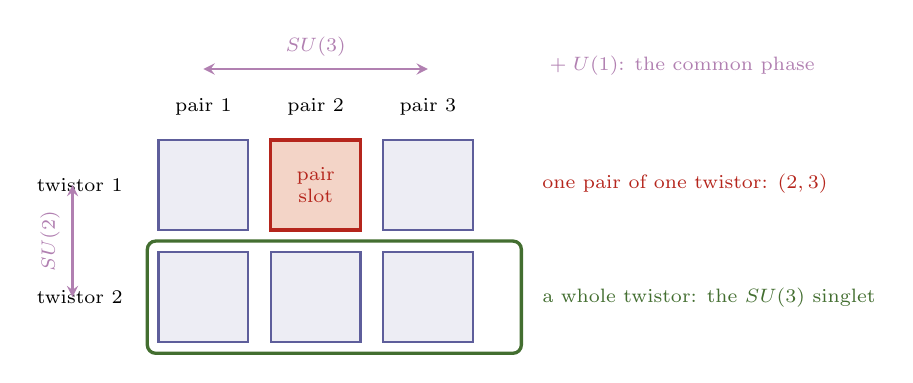
\begin{tikzpicture}[scale=0.95, >=stealth]
% the 2x3 grid of pairs
\foreach \i in {0,1} {
  \foreach \j in {0,1,2} {
    \draw[MidnightBlue!70, thick, fill=MidnightBlue!8]
      (\j*1.5, -\i*1.5) rectangle ++(1.2, 1.2);
  }
}
% highlight one cell: the pair-level generator (quark)
\draw[BrickRed, very thick, fill=BrickRed!15] (1.5, 0) rectangle ++(1.2, 1.2);
\node[BrickRed, font=\scriptsize, align=center] at (2.1, 0.6) {pair\\slot};
% highlight one row: the twistor-level generator (lepton)
\draw[OliveGreen!80!black, very thick, rounded corners=3pt]
  (-0.15, -1.65) rectangle (4.85, -0.15);
\node[OliveGreen!80!black, font=\scriptsize, anchor=west] at (5.0, -0.9)
  {a whole twistor: the $SU(3)$ singlet};
\node[BrickRed, font=\scriptsize, anchor=west] at (5.0, 0.62)
  {one pair of one twistor: $(2,3)$};
% axis labels
\node[font=\scriptsize, anchor=east] at (-0.35, 0.6) {twistor $1$};
\node[font=\scriptsize, anchor=east] at (-0.35, -0.9) {twistor $2$};
\node[font=\scriptsize] at (0.6, 1.65) {pair $1$};
\node[font=\scriptsize] at (2.1, 1.65) {pair $2$};
\node[font=\scriptsize] at (3.6, 1.65) {pair $3$};
% the automorphism arrows
\draw[<->, thick, Plum!80!black] (-1.15, 0.6) -- (-1.15, -0.9);
\node[Plum!80!black, font=\scriptsize, rotate=90] at (-1.45, -0.15) {$SU(2)$};
\draw[<->, thick, Plum!80!black] (0.6, 2.15) -- (3.6, 2.15);
\node[Plum!80!black, font=\scriptsize] at (2.1, 2.45) {$SU(3)$};
\node[Plum!80!black, font=\scriptsize] at (7.0, 2.2)
  {$+\; U(1)$: the common phase};
\end{tikzpicture}
\caption{The minimal massive hierarchy $\C^{2} \otimes \C^{3}$: two twistors (rows), each the vacuum of three ladder pairs (columns). The automorphisms respecting both levels of the partition are $SU(2)$ mixing the twistor slots, $SU(3)$ mixing the pair slots, and the common phase: the Standard Model algebra of Theorem \ref{thm:algebra}. The fermion generators are at the two levels (Proposition \ref{prop:content}): a pair-level generator occupies one cell and transforms as $(2,3)$, in the notation (dimension of the $SU(2)$ representation, dimension of the $SU(3)$ representation), the quark doublet; a twistor-level object enters a whole row as a unit; in the tensor state space the filled row is a quadruplet $(4,1)$ of hypercharge $+1/2$ (Proposition \ref{prop:content}(2)), and it becomes the lepton doublet $(2,1)$ of hypercharge $-1/2$ only under Hypothesis (S), where a row is one slot mode with the three pair modes occupied. A lepton is a complete twistor; a quark is a fractional one; and colour neutrality of the lepton is the figure's statement that a full row is an $SU(3)$ singlet.}
\label{fig:hierarchy}
\end{figure}

\begin{remark}[The eighth refutation: the split conclusion of the decisive test]\label{rem:eighth}
Comparing \eqref{eq:fock} with one Standard Model generation (the grid of Figure \ref{fig:hierarchy} is the object being decomposed) returns neither confirmation nor total failure but the framework's eighth refutation, a split conclusion. The exact agreement: the first excitation of the minimal massive hierarchy is $(2,3)$, the quark doublet, the Standard Model's most distinctive representation, appearing as the one-pair state. The near agreement: the massless sector's colour content $3 \oplus \bar{3} \oplus 1 \oplus 1$ against the observed $SU(2)$-singlet fields' $\bar{3} \oplus \bar{3} \oplus 1 \oplus 1$, a single conjugation of discrepancy, definite enough to be decided rather than debated. The definite disagreements: the lepton doublet $(2,1)$ appears nowhere in the raw spectrum; exotic representations appear that nature does not show (a colour sextet, an octet-doublet, an $SU(2)$ quadruplet); and the abelian charges are pair numbers, not hypercharges. The refutation relocates the test rather than ending it: the raw Fock space was never the physical spectrum, because elementary fermions are \emph{generators}, not states, and the corrected comparison is Proposition \ref{prop:content}'s. The list of disagreements is a specification of what the corrected comparison must supply.
\end{remark}

The comparison of Remark \ref{rem:eighth} set the Standard Model's elementary fermions against the state space's entire Fock space. The corrected comparison needs one definition and one declared hypothesis, stated here so that the propositions below are about defined objects and so that the reader can see exactly which results rest on which.

\emph{The hypercharge generator.} The Lie algebra of Theorem \ref{thm:global}'s group is $\mathfrak{s}(\uu(2) \oplus \uu(3)) = \{(X, X') : \tr X + \tr X' = 0\}$, and its centre is one-dimensional, spanned by
\[
\mathsf{y} := (3i\,I_{2},\; -2i\,I_{3}),
\]
the unique trace-free combination of the two scalar generators up to scale. The one-parameter subgroup $\exp(\theta\mathsf{y}) = (\lambda^{3}I_{2}, \lambda^{-2}I_{3})$, $\lambda = e^{i\theta}$, is the image of the $U(1)$ factor of Theorem \ref{thm:global}'s second isomorphism, so $\mathsf{y}$ acts on an irreducible constituent by $iq$ where $q$ is the abelian weight of Theorem \ref{thm:global}(ii). \emph{Hypercharge} is $Y := q/6$: the normalisation in which the lattice condition reads $t/3 + \delta/2 + Y \in \mathbb{Z}$, and in which, as computed below, a single pair has weight one unit. The sign of $\mathsf{y}$ is not fixed by the algebra: $(a, b, \lambda) \mapsto (\lambda^{-3}a, \lambda^{2}b)$ is an equally good second isomorphism with the same $\mathbb{Z}_{6}$ kernel, and it reverses every weight. The sign chosen here is the one in which the pair-level generators of Proposition \ref{prop:content}(1) have weight $+1$; the opposite sign gives the conjugate listing throughout, and the choice is part of the particle-antiparticle orientation of Theorem \ref{thm:hypercharge}(1). This is a definition of the symbol $Y$; that the symbol so defined is the hypercharge of the Standard Model is the observation-level identification of Theorem \ref{thm:algebra}'s reading, and is not claimed by the definition.

\emph{The tensor state space, and what it does not contain.} The state space of the minimal massive hierarchy is $\Lambda^{\bullet}(\C^{2} \otimes \C^{3})$, generated from its vacuum by the six creation operators of the cells of Figure \ref{fig:hierarchy}; a cell is one pair of one twistor, and an automorphism acts on the cells as $A \otimes B$. On this state space the $U(1)$ factor $(\lambda^{3}, \lambda^{-2})$ acts on a cell by $\lambda^{3}\lambda^{-2} = \lambda$, so a state with $k$ cells occupied has weight $k$, and Proposition \ref{prop:raw} lists every representation that occurs: $(2,3)$ at one cell, and in every degree only the representations of \eqref{eq:fock}. In particular no $(2,1)$ occurs anywhere in the tensor state space, and the states that fill a whole row of the figure, $(v \otimes f_{1}) \wedge (v \otimes f_{2}) \wedge (v \otimes f_{3})$ for $v \in \C^{2}$, are cubic in $v$ and span $S^{3}\C^{2} \otimes \Lambda^{3}\C^{3} = (4, 1)$, the quadruplet of Proposition \ref{prop:raw}'s degree three, of weight $+3$. A lepton doublet, $(2,1)$ of weight $-3$, is therefore not an object of the tensor state space, and no reading of its generators produces one. The same computation shows more: every cell has weight $+1$, so the state space contains no state of negative weight at all, and \eqref{eq:fock} contains no $(1, \bar{3})$ in any degree; so the single-twistor sector of Proposition \ref{prop:content}(3), with its negative weights $-2k$ and its $\bar{3}$ at grade two, is not a subspace of the tensor state space either. What is unconditional is the state space's own content, the quark doublet as its cells and the negative theorem; the single-twistor sector is a computation on the Fock space $\Lambda^{\bullet}W$ of one twistor's pairs, which under the hypothesis below is the slot-free row of one object holding both. The lepton needs a hypothesis, stated here.

\begin{quote}
\emph{Hypothesis (S), slot statistics.} The twistor slots of the composite are fermionic modes on the same footing as its pairs: the composite's state space is the Fock space $\Lambda^{\bullet}(\C^{2} \oplus W)$ of five modes, two slot modes and three pair modes, a state being a set of occupied slots and occupied pairs, on which $(A, B) \in U(2) \times U(3)$ acts as $\Lambda^{\bullet}(A \oplus B)$; and, as in Fact \ref{fact:pairs} for the three-mode Fock space $\Lambda^{\bullet}W$, the chirality of a state is the parity of its total mode number (Fact \ref{fact:fock} supplies the structure: $\Lambda^{\bullet}\C^{5}$ is the spinor module of $\Cl(10)$ and its parity grading is that module's chirality).
\end{quote}

Hypothesis (S) is a structural premise, not a theorem of the series, and the paper carries it as one: every result below that needs it says so, and successor problem (6) records what deciding it would settle and what it would cost. Two remarks on its content. Under (S) a cell of the tensor state space, one slot with one pair, is the state with one slot mode and one pair mode occupied, of weight $3 - 2 = 1$, so the pair-level content of the tensor state space is recovered; but (S) does not record which pairs belong to which slot, so it is not a refinement of the two-level hierarchy but a different state space with the same one-cell sector. And under (S) the automorphisms preserving the slot-pair split act faithfully: the kernel $K$ of Theorem \ref{thm:global} acts on the $(j, k)$ component by $\lambda^{j - k}$, so the automorphism group of the five-mode state space that preserves the slot-pair split and the mode number is $U(2) \times U(3)$ itself, thirteen-dimensional, and the framework's rule that the gauge group is the automorphism group then yields one abelian generator more than Theorem \ref{thm:algebra}'s twelve. The extra generator, the total mode number $j + k$ (or equivalently $j - k$), cannot be gauged: Proposition \ref{prop:sixteen}(3) proves that over the derived generation every abelian generator in the span of the two mode numbers except hypercharge fails three of the four anomaly conditions, so the automorphism rule read with anomaly cancellation returns the twelve. What (S) still costs is the second item: a state space that is not a refinement of the two-level hierarchy.

\begin{proposition}[Quarks and leptons: the two-level fermion content]\label{prop:content}
Under $S(U(2) \times U(3))$, with $Y$ the hypercharge just defined:
\begin{enumerate}
\item (Unconditional.) The pair-level generators, the cells of the tensor state space, transform as $(2, 3)$ with abelian weight $q = 1$, so $Y = 1/6$: the quark doublet's representation. A single pair has one unit of hypercharge.
\item (Under Hypothesis (S).) The states with one slot mode occupied and the pair modes in an $SU(3)$-invariant configuration are $\C^{2} \otimes \Lambda^{0}W$, weight $3$ ($Y = +1/2$, total mode number one, odd), and $\C^{2} \otimes \Lambda^{3}W$, weight $-3$ ($Y = -1/2$, total mode number four, even); both transform as $(2, 1)$. Without (S) neither exists in the state space, whose only row-filling states form the quadruplet $(4,1)$ of weight $+3$.
\item (Unconditional as a computation on the single-twistor Fock space, with the pair-slot factor acting alone; that Fock space is not a subspace of the tensor state space, and under (S) it is the row $j = 0$.) In the single-twistor sector $\Lambda^{\bullet}W = \Lambda^{\bullet}\C^{3}$, the grade-$k$ states transform as $\Lambda^{k}\C^{3}$, that is as $1, 3, \bar{3}, 1$ for $k = 0, 1, 2, 3$, with weight $q = -2k$: $Y = 0, -1/3, -2/3, -1$.
\end{enumerate}
In particular, under (S), the fermion content of the composite at the particle handedness (Theorem \ref{thm:hypercharge}) is
\begin{equation}\label{eq:content}
(2,3)_{1/6} \oplus (2,1)_{-1/2},
\end{equation}
quark doublet plus lepton doublet, with colour neutrality of the lepton the statement that a state with its pair modes full is an $SU(3)$ singlet: a lepton is a complete twistor, one slot with the pair system full, while a quark is one slot with one pair.
\end{proposition}

\begin{proof}
Write the $U(1)$ factor as $(A, B) = (\lambda^{3}a, \lambda^{-2}b)$ with $a \in SU(2)$, $b \in SU(3)$, as in Theorem \ref{thm:global}. (1) On $\C^{2} \otimes \C^{3}$ it acts as $\lambda^{3}\lambda^{-2}\,(a \otimes b) = \lambda\,(a \otimes b)$: the $SU(2) \times SU(3)$ content is $(2,3)$ and the weight is $3 - 2 = 1$, so $Y = 1/6$. (2) Under (S), $\Lambda^{\bullet}(\C^{2} \oplus W) = \bigoplus_{j,k}\Lambda^{j}\C^{2} \otimes \Lambda^{k}W$ (Fact \ref{fact:cauchy}), and on the $(j, k)$ component the $U(1)$ factor acts by $\lambda^{3j - 2k}$. The $SU(3)$-invariant lines of $\Lambda^{\bullet}W$ are $\Lambda^{0}W$ and $\Lambda^{3}W$ (Fact \ref{fact:pairs}), on which $b$ acts trivially; so the $(1, 0)$ component is $\lambda^{3}a \otimes 1$, content $(2,1)$, weight $3$, and the $(1, 3)$ component is $\lambda^{3}a \otimes \det(\lambda^{-2}b) = \lambda^{-3}a$, content $(2,1)$, weight $-3$. The negative clause: by Proposition \ref{prop:raw}, $(2,1)$ occurs in no degree of \eqref{eq:fock}; and the row-filling states are the image of the cubic map $v \mapsto \bigwedge_{a}(v \otimes f_{a})$, whose $SU(2)$-span is $S^{3}\C^{2} \otimes \Lambda^{3}\C^{3}$ (the map is the composite of $v \mapsto v^{\otimes 3}$ with the projection to $\Lambda^{3}$, and its image spans the symmetric cube), the $(4,1)$ of degree three, of weight $3$ since three cells are occupied. The script confirms this: with the unipotent $A(s)$ acting on the slot index, the transform of a filled row has components on four independent degree-three states with coefficients $s^{3}, s^{2}, s, 1$, so the $SU(2)$-span has rank four and is not a doublet. (3) The pair-slot factor alone acts on a single twistor's pair system, $\lambda^{-2}b$ on $W = \C^{3}$ (a lone twistor occupies no slot; under (S) this is the row $j = 0$, and without (S) it is the definition of the single-twistor sector); on $\Lambda^{k}W$ it acts as $\lambda^{-2k}\Lambda^{k}b$, so the content is $\Lambda^{k}\C^{3}$, which is $1, 3, \bar{3}, 1$ (Fact \ref{fact:cauchy}, $\Lambda^{2}\C^{3} \cong \bar{3}$), with weight $-2k$. Lattice membership, $2t + 3\delta + q \equiv 0 \pmod 6$: for (1), $t = 1$, $\delta = 1$, $q = 1$: $2 + 3 + 1 = 6$; for (2), $t = 0$, $\delta = 1$, $q = \pm 3$: $3 \pm 3 \in \{0, 6\}$; for (3), $(t, \delta, q) = (0, 0, 0), (1, 0, -2), (-1, 0, -4), (0, 0, -6)$: $0, 0, -6, -6$. The script builds the generator $\mathsf{y}$ as an exact matrix on each of these spaces and reads off the weights $1$, $3$, $-3$ and $0, -2, -4, -6$, and confirms the lattice residues.
\end{proof}

\begin{remark}[The weakness examined: exotics, conjugation, hypercharge]\label{rem:wound}
Three consequences, at three declared levels. First, at proposition level, the exotic representations of \eqref{eq:fock} are accounted for without projection: $(1,6)$, $(2,8)$, $(4,1)$ and their partners are multi-quantum states (the $(1,6)$ is a two-pair composite, the $(4,1)$ a full row) and are no more in need of removal from the elementary content than two-particle states are anywhere in quantum theory; Remark \ref{rem:eighth}'s miss list was a list of composites. What the tensor state space does not account for is the absence of the lepton, which is Hypothesis (S)'s to supply. Second, at open-question level, the single-twistor sector's colour content is $3 \oplus \bar{3}$ against the observed $\bar{3} \oplus \bar{3}$ of the two quark singlets, a single conjugation, which Proposition \ref{prop:chirality} resolves by the handedness of the listing; the particle-antiparticle orientation behind it is the descent's one undetermined bit, shown underivable in the dark-matter paper T14 \cite[Prop.~5.2]{ButlerT14}. Third, now at proposition level rather than observation level: the abelian weights are integers and $Y = q/6$, so hypercharge comes in units of $1/6$, the observed quantum, and under (S) the lepton-to-quark ratio $Y_{L}/Y_{Q} = -3$ is the pair count with the sign reversed, the full pair system having weight $-6$ against the empty one's $0$, added to the slot's $+3$. Theorem \ref{thm:hypercharge} completes the spectrum.
\end{remark}

\begin{theorem}[Hypercharge from the global form, pair counting, and consistency]\label{thm:hypercharge}
With $Y$ the hypercharge defined before Proposition \ref{prop:content}, and with Hypothesis (S) wherever a twistor-level doublet enters:
\begin{enumerate}
\item (Under (S).) The one-handed listing keeps the states of even total mode number and conjugates the odd ones, or the reverse; the choice is the particle-antiparticle orientation. Write $(j, k)$ for the component of the five-mode state space with $j$ slot modes and $k$ pair modes occupied (mode counts, not the pair of representation dimensions used elsewhere in this paper, for which see the caption of Figure \ref{fig:hierarchy}). In the listing that keeps the quark doublet, the component $(1,1)$, as a particle, the lepton doublet is the full twistor, the component $(1,3)$, $Y_{L} = -1/2$, and the empty twistor, the component $(1,0)$, appears only as its conjugate. The $[SU(2)]^{2}U(1)$ anomaly coefficient of the two doublets, $3Y_{Q} + Y_{L}$ with the three the colour multiplicity, is then the identity $3 \cdot \tfrac16 - \tfrac12 = 0$; it would equal $1$ if the empty twistor were listed as the particle instead, so the anomaly confirms the orientation the listing fixed. Pair counting fixes $|Y_{L}/Y_{Q}| = 3$; the parity fixes the sign.
\item (Unconditional as a computation on the single-twistor Fock space, like Proposition \ref{prop:content}(3).) Listed by the handedness of (1), the single-twistor sector gives the singlet spectrum. Here $\T = \Lambda^{\mathrm{even}}W$ and $\T' = \Lambda^{\mathrm{odd}}W$ are the two chirality halves (Fact \ref{fact:pairs}), and the listing keeping the even grades and conjugating the odd ones gives
\[
(1)_{0} \;\oplus\; (\bar{3})_{-2/3} \;\oplus\; (\bar{3})_{+1/3} \;\oplus\; (1)_{+1},
\]
that is $\nu^{c}$, $u^{c}$, $d^{c}$, $e^{c}$ with hypercharges $0, -\tfrac23, +\tfrac13, +1$: the observed singlet spectrum, with the fourth singlet at hypercharge zero. (The listing by the opposite handedness is the conjugate of this one, the same spectrum in the opposite convention.) Under (S) the single-twistor grade-$k$ states are the $(0, k)$ components, the states with no slot mode and $k$ pair modes occupied (their content $\Lambda^{k}\C^{3}$ and weight $-2k$ match, and irreducibles are determined by content and weight), so their parity is the total parity and this listing is the same listing as in (1).
\item (Consistency, and uniqueness given the content; under (S) for the doublets.) With the content of (1) and (2), all four anomaly conditions of Fact \ref{fact:anomaly} hold. Conversely, for the field content $Q = (2,3)$, $L = (2,1)$, $u^{c} = (1,\bar{3})$, $d^{c} = (1,\bar{3})$, $e^{c} = (1,1)$, all listed in one handedness, together with a fourth singlet of hypercharge zero or no fourth singlet, and $Y_{Q} = 1/6$ as the normalisation, the four conditions determine $Y_{L}$, $Y(e^{c})$ and $\{Y(u^{c}), Y(d^{c})\}$ uniquely, and the solution is the spectrum of (1) and (2). Both hypotheses are necessary: with a fourth singlet of unconstrained hypercharge the conditions admit a one-parameter family, and if the doublets were listed in the opposite handedness from the singlets the $[SU(3)]^{2}U(1)$ and cubic sums would be $-\tfrac23$ and $+\tfrac49$ rather than zero.
\end{enumerate}
\end{theorem}

\begin{proof}
(1) Under (S) the states of Proposition \ref{prop:content}(1) and (2) have total mode numbers $2$, $1$ and $4$ for $(1,1)$, $(1,0)$ and $(1,3)$, and by (S) the chirality is the parity; so $(1,1)$ and $(1,3)$ share a handedness and $(1,0)$ has the other. By Fact \ref{fact:anomaly}'s convention a state of the opposite handedness is listed as its conjugate, so the listing that keeps the component $(1,1)$ keeps the component $(1,3)$ and conjugates the component $(1,0)$ to $(2,1)_{-1/2}$, the same representation as the component $(1,3)$ (Proposition \ref{prop:chirality}). The $[SU(2)]^{2}U(1)$ coefficient is the sum of $Y$ over the doublets weighted by colour multiplicity: $3 \cdot \tfrac16 + (-\tfrac12) = 0$ for the listing above, and $3 \cdot \tfrac16 + \tfrac12 = 1$ for the listing that keeps $(1,0)$ and conjugates $(1,3)$.

(2) Proposition \ref{prop:content}(3) gives the single-twistor states as $(1)_{0}$ at grade $0$, $(3)_{-1/3}$ at grade $1$, $(\bar{3})_{-2/3}$ at grade $2$ and $(1)_{-1}$ at grade $3$. The even grades lie in $\T$ and the odd grades in $\T'$, the two chirality halves of Fact \ref{fact:pairs}. Conjugating the odd ones, with the conjugate representation and the opposite hypercharge: $(3)_{-1/3} \mapsto (\bar{3})_{+1/3}$ and $(1)_{-1} \mapsto (1)_{+1}$. The even grades are unchanged. This is the display. Under (S) the grade-$k$ single-twistor state is the $(0, k)$ component, of total mode number $k$, so the parity used here is the parity of (1).

(3) Consistency. $[SU(3)]^{2}U(1)$: the triplets and antitriplets are $Q$ (multiplicity two) and $u^{c}$, $d^{c}$: $2 \cdot \tfrac16 - \tfrac23 + \tfrac13 = 0$. $[SU(2)]^{2}U(1)$: (1). Gravitational: $6 \cdot \tfrac16 + 2 \cdot (-\tfrac12) + 3 \cdot (-\tfrac23) + 3 \cdot \tfrac13 + 1 + 0 = 1 - 1 - 2 + 1 + 1 = 0$. Cubic: $6 \cdot \tfrac{1}{216} + 2 \cdot (-\tfrac18) + 3 \cdot (-\tfrac{8}{27}) + 3 \cdot \tfrac{1}{27} + 1 + 0 = \tfrac{1}{36} - \tfrac14 - \tfrac89 + \tfrac19 + 1 = 0$. Uniqueness. Write $Y_{Q} = a = \tfrac16$, $Y(u^{c}) = b$, $Y(d^{c}) = c$, $Y_{L} = d$, $Y(e^{c}) = e$, and $f$ for the fourth singlet, with $f = 0$ or absent. $[SU(2)]^{2}U(1)$: $3a + d = 0$, so $d = -\tfrac12$. $[SU(3)]^{2}U(1)$: $2a + b + c = 0$, so $b + c = -\tfrac13$. Gravitational: $6a + 3b + 3c + 2d + e + f = 1 - 1 - 1 + e = 0$, so $e = 1$. Cubic: $6a^{3} + 3(b^{3} + c^{3}) + 2d^{3} + e^{3} + f^{3} = \tfrac{1}{36} - \tfrac14 + 3(b^{3} + c^{3}) + 1 = 0$, so $b^{3} + c^{3} = -\tfrac{7}{27}$; with $s = b + c = -\tfrac13$ and $p = bc$, the identity $b^{3} + c^{3} = s^{3} - 3ps$ gives $-\tfrac{1}{27} + p = -\tfrac{7}{27}$, so $p = -\tfrac29$, and $b, c$ are the roots of $y^{2} + \tfrac13 y - \tfrac29 = 0$, namely $(-\tfrac13 \pm 1)/2 = \{+\tfrac13, -\tfrac23\}$. Unique. Necessity of the fourth-singlet hypothesis: if $f$ is free, the gravitational and cubic conditions constrain $e + f$ and $e^{3} + f^{3}$ together and no longer fix $e$. Explicitly, $(a, b, c, d, e, f) = (\tfrac16, -\tfrac16, -\tfrac16, -\tfrac12, \tfrac12, \tfrac12)$ satisfies all four conditions ($b + c = -\tfrac13$; $d = -\tfrac12$; $1 - 1 - 1 + \tfrac12 + \tfrac12 = 0$; $\tfrac{1}{36} - \tfrac{1}{36} - \tfrac14 + \tfrac18 + \tfrac18 = 0$), and it is not isolated: $Y + t(B - L)$, with $B - L$ the baryon-minus-lepton charge ($\tfrac13$ on $Q$, $-\tfrac13$ on $u^{c}$, $d^{c}$, $-1$ on $L$, $1$ on $e^{c}$ and on the fourth singlet), solves the four conditions for every $t$: each of the four sums is a polynomial of degree at most three in $t$, so vanishing at four values of $t$ is vanishing identically; the script confirms the vanishing at $t = 0$ (the derived spectrum), at $t = 1, -1, 2$, and at $t = \tfrac57$. (Rescaling a member to $Y_{Q} = \tfrac16$, possible for $t \neq -\tfrac12$ where $Y_{Q} = \tfrac16 + \tfrac{t}{3}$ vanishes, multiplies the three linear sums by a constant and the cubic one by its cube, so preserves vanishing; the argument is run on the unrescaled family.) The exhibited point is the $t \to \infty$ limit of the family, rescaled. With $f = 0$ imposed, or the fourth singlet absent, the family collapses to the single solution above. Necessity of the common handedness: conjugating the two doublets alone sends $(a, d)$ to $(-\tfrac16, \tfrac12)$ in the conjugate representations, and the four sums become $[SU(3)]^{2}U(1) = -2a + b + c = -\tfrac23$, $[SU(2)]^{2}U(1) = -3a - d = 0$, gravitational $-6a + 3b + 3c - 2d + e = 0$, cubic $-6a^{3} + 3(b^{3} + c^{3}) - 2d^{3} + e^{3} = +\tfrac49$. Every line of this arithmetic is verified exactly by the script.
\end{proof}

\begin{proposition}[Chirality: the two halves of the spinor module, and conjugation as duality]\label{prop:chirality}
The twistor space $\T = \Lambda^{\mathrm{even}}W$ and its partner $\T' = \Lambda^{\mathrm{odd}}W$ are the two chirality halves of the ascended Dirac module (Fact \ref{fact:pairs}), and the single-twistor sector $\Lambda^{\bullet}W$ is their direct sum. Under $S(U(2) \times U(3))$ the two halves carry different content: $\T$ carries $(1)_{0} \oplus (\bar{3})_{-2/3}$ and $\T'$ carries $(3)_{-1/3} \oplus (1)_{-1}$ (Proposition \ref{prop:content}(3)), so the two halves are inequivalent representations of the group: the chirality split is visible to the internal symmetry, not only to the grading. The singlet spectrum listed by a single handedness is Theorem \ref{thm:hypercharge}(2)'s, and in particular the colour content $3 \oplus \bar{3}$ of the two halves becomes $\bar{3} \oplus \bar{3}$ under it, which is the conjugation of Remark \ref{rem:wound}. Moreover the conjugation is an operation inside the pair system: the dual of the grade-$k$ state is the grade-$(3-k)$ state with the full-system phase removed, $(\Lambda^{k}W)^{*} \cong \Lambda^{3-k}W \otimes (\Lambda^{3}W)^{*}$, of weight $+2k$; and the two twistor-level doublets of Proposition \ref{prop:content}(2) are each other's duals, $(\C^{2} \otimes \Lambda^{0}W)^{*} \cong \C^{2} \otimes \Lambda^{3}W$, and under (S) have opposite parity. Under (S) they are therefore one doublet and its antiparticle, not two candidates, and Theorem \ref{thm:hypercharge}(1)'s listing choice is the particle-antiparticle orientation of Remark \ref{rem:wound}.
\end{proposition}

\begin{proof}
The chirality statement is Fact \ref{fact:pairs}. The content of each half is Proposition \ref{prop:content}(3) sorted by parity of grade: even grades $0$ and $2$ give $(1)_{0}$ and $(\bar{3})_{-2/3}$; odd grades $1$ and $3$ give $(3)_{-1/3}$ and $(1)_{-1}$. The two halves are inequivalent as representations (their $SU(3)$ contents $1 \oplus \bar{3}$ and $3 \oplus 1$ differ, and so do their weight sets $\{0, -4\}$ and $\{-2, -6\}$), so no intertwiner exists. The one-handed listing is Theorem \ref{thm:hypercharge}(2); conjugating the odd half turns its $3$ into $\bar{3}$, so the colour content becomes $\bar{3} \oplus \bar{3}$. The duality: by Fact \ref{fact:cauchy}, $(\Lambda^{k}W)^{*} \cong \Lambda^{3-k}W \otimes \det^{-1}$ as $U(3)$-modules, and under $B = \lambda^{-2}b$ the right side has weight $-2(3-k) + 6 = 2k$, the negative of the grade-$k$ weight, as a dual must. For the doublets, $(\C^{2})^{*} \cong \C^{2} \otimes \det(A)^{-1}$ as a $U(2)$-module (the $2$ of $SU(2)$ is self-dual, $\varepsilon$ being the intertwiner), and under $A = \lambda^{3}a$ this has weight $3 - 6 = -3$ with $SU(2) \times SU(3)$ content $(2, 1)$, which is the content and weight of $\C^{2} \otimes \Lambda^{3}W$; irreducible representations of $S(U(2) \times U(3))$ are determined by their $SU(2)$ content, $SU(3)$ content and abelian weight (they are the irreducibles of $SU(2) \times SU(3) \times U(1)$ trivial on $\mathbb{Z}_{6}$), so the two are isomorphic. Their total mode numbers under (S) are $1$ and $4$, of opposite parity. The script checks the weights $+2k$ and $-3$ on the explicit duals.
\end{proof}

At observation level, and flagged as such: the weak coupling is chiral because the automorphisms act on states of definite chirality, and under (S) every state of the composite has one, the parity of its mode number; which parity is called left-handed is the identification of the one-handed listing of Theorem \ref{thm:hypercharge} with the Standard Model's left-handed convention, and it is the same choice as the orientation. That twistor charge is helicity (Fact \ref{fact:helicity}) is what ties the parity of the single-twistor sector to spacetime handedness; the extension of that tie to the five-mode parity of (S) is part of what (S) asserts.

\begin{proposition}[The connection is forced]\label{prop:connection}
Let matter fields be sections of $\mathcal{S} \otimes \mathcal{H}$ over spacetime, with $\mathcal{S}$ the local twistor bundle of Fact \ref{fact:tractor} (the spinor bundle of the tractor bundle, whose fibres are the twistors) and $\mathcal{H}$ the hierarchy bundle, a complex vector bundle of rank six whose fibres carry the factorisation $\C^{2} \otimes \C^{3}$ and its Hermitian structure. Let $D$ be a connection on $\mathcal{S} \otimes \mathcal{H}$ that is induced from connections on the two factors, $D = \nabla \otimes 1 + 1 \otimes D_{\mathcal{H}}$, with $\nabla$ a $\mathrm{Spin}(2,4)$-connection on $\mathcal{S}$ (one whose transports lie in the spin group acting on the twistor fibre, as local twistor transport does) and $D_{\mathcal{H}}$ preserving the Hermitian structure and the factorisation of the fibre (its parallel transports map the set of decomposable tensors onto itself). Then $\nabla$ has connection form valued in $\mathfrak{so}(2,4)$ and $D_{\mathcal{H}} = d + \mathcal{A}$ in any factorisation-adapted local frame, with $\mathcal{A}$ a one-form valued in $\su(2) \oplus \su(3) \oplus \uu(1)$ acting through Theorem \ref{thm:algebra}'s action; conversely every such pair $(\nabla, \mathcal{A})$ gives a connection with these properties.
\end{proposition}

\begin{proof}
A connection on a vector bundle whose parallel transports lie in a closed subgroup $G$ of the fibre's general linear group has, in a local frame adapted to $G$, a connection form valued in the Lie algebra of $G$: the transport along a curve $\gamma$ from $\gamma(0)$ to $\gamma(t)$ is a curve in $G$ through the identity, differentiable in $t$ since the connection is smooth, and the connection form evaluated on $\dot\gamma(0)$ is its derivative at $t = 0$, a tangent vector to $G$ at the identity; that a closed subgroup is an embedded Lie subgroup, so that this tangent vector lies in its Lie algebra, is the closed-subgroup theorem \cite[Thm.~20.12]{Lee2013}. For $\nabla$ the group is $\mathrm{Spin}(2,4)$, with Lie algebra $\mathfrak{so}(2,4)$ (Fact \ref{fact:tractor}); this half of the statement is the hypothesis read through that theorem. For $D_{\mathcal{H}}$ the transports are unitary maps of $\C^{2} \otimes \C^{3}$ carrying the set of decomposable tensors onto itself, hence of the form $A \otimes B$ with $(A, B) \in U(2) \times U(3)$ by Lemma \ref{lem:segre} ($m = 2 \neq 3 = k$); the group of such maps is the image of $U(2) \times U(3)$, closed since $U(2) \times U(3)$ is compact, with Lie algebra the image of $\uu(2) \oplus \uu(3)$ under $(X, X') \mapsto X \otimes 1 + 1 \otimes X'$, which is $\su(2) \oplus \su(3) \oplus \uu(1)$ acting as in Theorem \ref{thm:algebra}. Conversely a connection form valued in a Lie algebra $\mathfrak{g}$ has transports in the connected group generated by $\exp\mathfrak{g}$, which preserves whatever $\mathfrak{g}$ infinitesimally preserves: the spin structure for $\mathfrak{so}(2,4)$, and the decomposable tensors and the Hermitian structure for the image of $\uu(2) \oplus \uu(3)$, since $\exp(X \otimes 1 + 1 \otimes X') = e^{X} \otimes e^{X'}$.
\end{proof}

At observation level, and flagged as such: minimal coupling is on this reading a holonomy constraint rather than an ansatz, the gauge fields of the Standard Model algebra being exactly the freedom to rotate the pair hierarchy independently from point to point. The gauging of the internal factors is Yang-Mills, not MacDowell-Mansouri, by Fact \ref{fact:twokinds}: the internal forces are conformal-level, gravity alone is pre-metric, and the $\theta$-terms are what survives the singularity. The coupling constants $g_{i}$ are normalisations this proposition does not determine; the numerical layer of Section \ref{sec:running} takes them up. Under Hypothesis (S) the hierarchy bundle would have fibre $\Lambda^{\bullet}(\C^{2} \oplus W)$ and the split-and-number-preserving structure group $U(2) \times U(3)$, with the thirteenth generator settled in Proposition \ref{prop:sixteen}(3); the proposition as stated is the tensor state space's.

\begin{proposition}[Under (S): the composite's state space is the $\mathrm{Spin}(10)$ spinor, and the derived generation is its even half]\label{prop:sixteen}
Assume Hypothesis (S). Let $S(U(2) \times U(3))$ act on $\Lambda^{\bullet}(\C^{2} \oplus \C^{3})$ through $\Lambda^{\bullet}(A \oplus B)$, so that on the component $\Lambda^{j}\C^{2} \otimes \Lambda^{k}\C^{3}$ the abelian factor $\lambda$ acts by $\lambda^{3j - 2k}$. Then:
\begin{enumerate}
\item The one-generation spectrum of Theorem \ref{thm:hypercharge},
\[
Q \oplus L \oplus u^{c} \oplus d^{c} \oplus e^{c} \oplus \nu^{c}
\;=\; (2,3)_{1/6} \oplus (2,1)_{-1/2} \oplus (1,\bar{3})_{-2/3} \oplus (1,\bar{3})_{1/3} \oplus (1,1)_{1} \oplus (1,1)_{0},
\]
is exactly the even part $\Lambda^{\mathrm{even}}(\C^{2} \oplus \C^{3})$, sixteen-dimensional, with $\nu^{c}$, $u^{c}$, $Q$, $L$, $e^{c}$, $d^{c}$ at $(j, k) = (0,0), (0,2), (1,1), (1,3), (2,0), (2,2)$; and the odd part $\Lambda^{\mathrm{odd}}(\C^{2} \oplus \C^{3})$ is its dual, the antiparticles, with the empty-twistor doublet $(2,1)_{1/2}$ at $(1,0)$. The mass bracket's slot factor $\Lambda^{2}\C^{2}$, $(1,1)_{1}$, is the even component $(2,0)$, the same representation as $e^{c}$.
\item The five-mode Fock space $\Lambda^{\bullet}(\C^{2} \oplus \C^{3}) = \Lambda^{\bullet}\C^{5}$ is the spinor module of $\Cl(10)$, its two parities are the two half-spinor representations of $\mathrm{Spin}(10)$, and the automorphisms of the five-mode state space's canonical anticommutation relations induced by orthogonal maps of its ten Majorana generators form $O(10)$, implemented on the Fock space by $\mathrm{Pin}(10)$, with the connected part $SO(10)$ implemented by $\mathrm{Spin}(10)$ (Fact \ref{fact:fock}). The derived generation is therefore the half-spinor $16$ of $\mathrm{Spin}(10)$ restricted to $S(U(2) \times U(3))$, with the twistor slots as two of the five modes and the pairs as the other three; the automorphisms preserving in addition the mode number form $U(5)$, and those preserving the slot-pair split as well form $U(2) \times U(3)$, of which Theorem \ref{thm:global}'s group is the determinant-one part. (The number-preserving subgroup of $\mathrm{Spin}(10)$ is a double cover of $U(5)$ acting as $\Lambda^{\bullet} \otimes \det^{-1/2}$, the "determinant phase" of Fact \ref{fact:fock}; the action $\Lambda^{\bullet}(A \oplus B)$ declared above is that of $U(2) \times U(3) \subset SO(10)$, and the two agree on the determinant-one subgroup, where every hypercharge of this paper is computed.)
\item Among the abelian generators of the split-and-number-preserving algebra, acting on the component $(j,k)$ by $\alpha j + \beta k$ with $\alpha, \beta$ real (hypercharge being $(\alpha, \beta) = (\tfrac12, -\tfrac13)$, the pair $(3,-2)$ divided by six):
\begin{enumerate}
\item[(a)] in the action $\Lambda^{\bullet}(A \oplus B)$ declared above, the $[SU(3)]^{2}U(1)$, $[SU(2)]^{2}U(1)$ and gravitational sums of Fact \ref{fact:anomaly} over the derived generation are $2(2\alpha + 3\beta)$, $2(2\alpha + 3\beta)$ and $8(2\alpha + 3\beta)$, and the cubic sum is a cubic form in $(\alpha, \beta)$ vanishing at $(3,-2)$; so the three linear conditions hold if and only if the generator is a multiple of hypercharge, the total mode number $j + k$ having sums $(10, 10, 40, 400)$ and $j - k$ having $(-2, -2, -8, -32)$;
\item[(b)] in the action the state space carries, that of $\mathrm{Spin}(10)$ through $\Lambda^{\bullet} \otimes \det^{-1/2}$ in (2), the generator acts by $\alpha j + \beta k - \tfrac12(2\alpha + 3\beta)$, and all four sums, together with the mixed sums $Y^{2}X$ and $YX^{2}$ with hypercharge, vanish for every $(\alpha, \beta)$.
\end{enumerate}
The thirteenth generator of the five-mode state space's automorphism algebra is therefore anomaly-free in the action the generation carries. It is
\[
X \;=\; j + k - \tfrac52 \;=\; 2Y - \tfrac52\,(B - L), \qquad B - L \;:=\; 1 - \tfrac23\,k,
\]
the pair-number form of the operator $B - L$ of Fact \ref{fact:gj}, and it takes the values $-\tfrac52$ on $\nu^{c}$, $-\tfrac12$ on $Q$, $u^{c}$, $e^{c}$ and $\tfrac32$ on $L$, $d^{c}$: the $U(1)_{X}$ of $\mathrm{Spin}(10)$. The automorphism rule of Theorem \ref{thm:algebra}, read with anomaly cancellation, returns thirteen generators. The thirteenth is broken by the right-handed neutrino's Majorana bilinear $\nu^{c}\nu^{c}$, which carries $X = -5$ and $B - L = 2$ (Proposition \ref{prop:breaking}), and the twelve are what survives below that scale.
\end{enumerate}
Without (S) the first statement is a theorem about a spectrum and an exterior algebra that happen to coincide, with the exterior algebra an object the paper never built; the second is Fact \ref{fact:fock} instantiated and is not available; the third is a computation on the table of components and is not needed.
\end{proposition}

\begin{proof}
(1) By Fact \ref{fact:cauchy}, $\Lambda^{n}(\C^{2} \oplus \C^{3}) = \bigoplus_{j+k=n}\Lambda^{j}\C^{2} \otimes \Lambda^{k}\C^{3}$, and $(A, B) = (\lambda^{3}a, \lambda^{-2}b)$ acts on $\Lambda^{j}\C^{2} \otimes \Lambda^{k}\C^{3}$ as $\lambda^{3j}\lambda^{-2k}\,\Lambda^{j}a \otimes \Lambda^{k}b$. The twelve components, with $\Lambda^{0}\C^{2} = \Lambda^{2}\C^{2} = 1$, $\Lambda^{1}\C^{2} = 2$, and $\Lambda^{0,1,2,3}\C^{3} = 1, 3, \bar{3}, 1$ under $SU(2) \times SU(3)$, with weight $3j - 2k$ and $Y = (3j-2k)/6$:
\[
\begin{array}{c|cccc}
j \backslash k & 0 & 1 & 2 & 3 \\ \hline
0 & (1,1)_{0} & (1,3)_{-1/3} & (1,\bar{3})_{-2/3} & (1,1)_{-1} \\
1 & (2,1)_{1/2} & (2,3)_{1/6} & (2,\bar{3})_{-1/6} & (2,1)_{-1/2} \\
2 & (1,1)_{1} & (1,3)_{2/3} & (1,\bar{3})_{1/3} & (1,1)_{0}
\end{array}
\]
The even components ($j + k$ even) are $(0,0) = \nu^{c}$, $(0,2) = u^{c}$, $(1,1) = Q$, $(1,3) = L$, $(2,0) = e^{c}$, $(2,2) = d^{c}$, exactly the six representations of Theorem \ref{thm:hypercharge} with their hypercharges, and irreducibles of $S(U(2) \times U(3))$ are determined by content and weight (proof of Proposition \ref{prop:chirality}), so the even part is the derived generation; its dimension is $1 + 3 + 6 + 2 + 1 + 3 = 16$. The odd components are $(0,1) = (1,3)_{-1/3}$, $(0,3) = (1,1)_{-1}$, $(1,0) = (2,1)_{1/2}$, $(1,2) = (2,\bar{3})_{-1/6}$, $(2,1) = (1,3)_{2/3}$, $(2,3) = (1,1)_{0}$, the duals of $d^{c}$, $e^{c}$, $L$, $Q$, $u^{c}$, $\nu^{c}$ respectively (conjugate content, opposite weight); the map $(j, k) \mapsto (2 - j, 3 - k)$, the Hodge star of the exterior algebra, realises the duality and negates the weight, $3(2-j) - 2(3-k) = -(3j - 2k)$. The $(2,0)$ entry is $\Lambda^{2}\C^{2} = \det$, the slot factor of Proposition \ref{prop:singlet}. (2) is Fact \ref{fact:fock} with $n = 5$, together with the observation that the split-preserving, number-preserving automorphisms of the five modes are the unitaries of $\C^{2} \oplus \C^{3}$ preserving the summands, $U(2) \times U(3)$; the parenthesis is the "determinant phase" clause of that Fact, and the twist $\det^{-1/2}$ is trivial where $\det(A \oplus B) = 1$. (3) Over the even components, the generator's values are $\nu^{c}$: $0$; $u^{c}$: $2\beta$; $Q$: $\alpha + \beta$; $L$: $\alpha + 3\beta$; $e^{c}$: $2\alpha$; $d^{c}$: $2\alpha + 2\beta$. With Fact \ref{fact:anomaly}'s sums in the form used in the proof of Theorem \ref{thm:hypercharge}(3), $Q$ entering the $SU(3)$ sum twice and the gravitational and cubic sums six times, $L$ twice, and the singlets by their colour multiplicity: $[SU(3)]^{2}U(1) = 2(\alpha + \beta) + 2\beta + (2\alpha + 2\beta) = 4\alpha + 6\beta$; $[SU(2)]^{2}U(1) = 3(\alpha + \beta) + (\alpha + 3\beta) = 4\alpha + 6\beta$; gravitational $= 6(\alpha + \beta) + 3 \cdot 2\beta + 3(2\alpha + 2\beta) + 2(\alpha + 3\beta) + 2\alpha = 16\alpha + 24\beta$; cubic $= 6(\alpha + \beta)^{3} + 3(2\beta)^{3} + 3(2\alpha + 2\beta)^{3} + 2(\alpha + 3\beta)^{3} + (2\alpha)^{3}$, which at $(3, -2)$ is $6 - 192 + 24 - 54 + 216 = 0$, at $(1, 1)$ is $48 + 24 + 192 + 128 + 8 = 400$, and at $(1, -1)$ is $0 - 24 + 0 - 16 + 8 = -32$. The three linear sums are multiples of $2\alpha + 3\beta$, so vanish together exactly on the line through $(3,-2)$; on that line the cubic sum is a cubic in one variable vanishing at $(3,-2)$, hence identically. The script evaluates all four sums for every integer pair $(\alpha, \beta) \in [-6, 6]^{2}$ and finds the three linear ones vanishing exactly at the multiples of $(3, -2)$. For (b): the twist subtracts $\tfrac12(2\alpha + 3\beta)$ from every entry, which removes the three linear sums exactly, since they count four, four and sixteen entries; the cubic and the two mixed sums become polynomials of degree at most three in each of $\alpha$ and $\beta$, which the script finds vanishing on a five-by-five grid of rational points, hence identically. That nothing in $\mathrm{Spin}(10)$ is anomalous on the $16$ is also the standard statement that $SO(10)$ has no cubic invariant. The values of $X$ and the identity $X = 2Y - \tfrac52(B - L)$ are read off the table of (1), species by species. The script builds the hypercharge generator as an exact matrix on all thirty-two dimensions of $\Lambda^{\bullet}(\C^{2} \oplus \C^{3})$, reads off the weight on each component, confirms that the even components' (content, weight) multiset is the derived spectrum's and that the odd components' is its conjugate, and confirms that the Hodge star negates the weight on all twelve components.
\end{proof}

\begin{remark}[Point of contact: grand unification, and what Hypothesis (S) would yield and what it would cost]\label{rem:sixteen}
$\Lambda^{\mathrm{even}}\C^{5}$ restricted to $S(U(2) \times U(3)) \subset SU(5) \subset \mathrm{Spin}(10)$ being one Standard Model generation with a right-handed neutrino is the exterior-algebra presentation of grand unification expounded by Baez and Huerta \cite{BaezHuerta2010}, and Proposition \ref{prop:sixteen} arrives at it with the twistor-slot space as the $\C^{2}$ summand, the pair space $W$ as the $\C^{3}$ summand, and the duality of Proposition \ref{prop:chirality} as its Hodge star. What Hypothesis (S) would yield: the group $\mathrm{Spin}(10)$ is then the framework's own, the automorphism group of the composite's state space in the same sense in which $S(U(2) \times U(3))$ is the automorphism group of the two-level partition, and the hypothesis of Fact \ref{fact:running}(b) is discharged with $G_{U} = \mathrm{Spin}(10)$ and the derived generation as its $16$, so that $3/8$ becomes a derived value rather than an inherited one. What it would cost, stated before Proposition \ref{prop:content}: the automorphisms preserving the split and the mode number are $U(2) \times U(3)$, thirteen-dimensional, so the automorphism rule that gave twelve generators in Theorem \ref{thm:algebra} gives thirteen under (S); the extra abelian generator is anomaly-free in the action the generation carries (Proposition \ref{prop:sixteen}(3)), so the rule returns thirteen generators and the thirteenth must be broken, which the right-handed neutrino's Majorana mass does (Proposition \ref{prop:breaking}); and the five-mode state space does not record which pairs belong to which slot, so the two-level hierarchy of Section \ref{sec:algebra} is not a substructure of it. Deciding (S) is successor problem (6), and it is the decision on which the lepton, the singlet listing as part of one object, the unification group and the values $3/8$ and $3/4$ all turn.
\end{remark}

\section{Unification and the desert}\label{sec:running}

The three couplings $g_{1}, g_{2}, g_{3}$ are the normalisations Proposition \ref{prop:connection} left free. At observation level, and flagged as such, the framework suggests a reason they should meet: all three factors act on one fibre. But this is not a proof, and the paper does not offer it as one. The invariant symmetric forms on $\su(2) \oplus \su(3) \oplus \uu(1)$ form a three-parameter family, one scale per summand, so ``one trace normalisation'' on the fibre picks one member of the family and does not privilege it; the trace form of $\C^{2} \otimes \C^{3}$ itself, restricted to the algebra, gives $\sum T_{3}^{2}/\sum Q^{2} = 9/10$ over the fibre, unconditionally, and $3/4$ over the two doublets alone, which needs Hypothesis (S) for the lepton doublet (both computed in the proof below), neither of them the unification value. What forces a normalisation is a simple unifying group, Fact \ref{fact:running}(b), whose existence the framework derives only under Hypothesis (S), where Proposition \ref{prop:sixteen}(2) supplies $\mathrm{Spin}(10)$; without (S), Theorem \ref{thm:global}(i) says only that the global form is the one such an embedding requires. The unification hypothesis is therefore imported here at assembly level, with the note that (S) would discharge it, and the trace ratio is computed over the content of Theorem \ref{thm:hypercharge}.

\begin{proposition}[The weak angle over the derived generation]\label{prop:unification}
Over one generation of the content of Theorem \ref{thm:hypercharge}, quark and lepton doublets and the four singlets (the lepton under Hypothesis (S)), with $Q = T_{3} + Y$,
\begin{equation}\label{eq:angle}
\frac{\sum T_{3}^{2}}{\sum Q^{2}} \;=\; \frac{2}{2 + \tfrac{10}{3}} \;=\; \frac{3}{8},
\end{equation}
and this is $\sin^{2}\theta_{W}$ at the unification scale under the hypothesis of Fact \ref{fact:running}(b), the classic value, here over derived rather than assumed content. The value rests on (S) with the lepton doublet, which contributes $\tfrac12$ to each sum: over the unconditional content alone, the quark doublet and the four singlets, the same ratio is $9/26$. Over the fibre $\C^{2} \otimes \C^{3}$ alone the ratio is $9/10$, unconditionally, and over the two doublets alone $3/4$, again under (S). Comparison with the observed $0.2312$ requires renormalisation-group running from the unification scale (the structural scale $M_{U}$), which Proposition \ref{prop:desert} performs.
\end{proposition}

\begin{proof}
The sums over the Weyl fermions of one derived generation: $\sum T_{3}^{2} = 3 \cdot 2 \cdot \tfrac14 + 2 \cdot \tfrac14 = \tfrac32 + \tfrac12 = 2$ (quark doublet with colour multiplicity, lepton doublet; the singlets have $T_{3} = 0$); $\sum Y^{2} = 6 \cdot \tfrac{1}{36} + 2 \cdot \tfrac14 + 3 \cdot \tfrac49 + 3 \cdot \tfrac19 + 1 + 0 = \tfrac16 + \tfrac12 + \tfrac43 + \tfrac13 + 1 = \tfrac{10}{3}$ (doublets, then $u^{c}, d^{c}, e^{c}, \nu^{c}$); and the cross term $2\sum T_{3}Y$ vanishes because each doublet's $T_{3}$ values sum to zero at fixed $Y$. Hence $\sum Q^{2} = 2 + \tfrac{10}{3} = \tfrac{16}{3}$ and the ratio is $\tfrac38$. Under Fact \ref{fact:running}(b) the ratio over any representation of the unifying group is $\sin^{2}\theta_{W}$ at the unification scale; that one generation of this content, with the hypercharge-zero singlet, is a representation of a simple group containing $S(U(2) \times U(3))$ is Proposition \ref{prop:sixteen}(1) with Fact \ref{fact:fock} (the $16$ of $\mathrm{Spin}(10)$, whose restriction to $SU(5) \supset S(U(2) \times U(3))$ is $\bar{5} \oplus 10 \oplus 1$), and the ratio computed here is the same over $\bar{5} \oplus 10$, since the singlet contributes nothing to either sum. Without the lepton: $\sum T_{3}^{2} = \tfrac32$, $\sum Y^{2} = \tfrac{10}{3} - \tfrac12 = \tfrac{17}{6}$, $\sum Q^{2} = \tfrac{13}{3}$, ratio $\tfrac{9}{26}$. Over the fibre alone: $\sum T_{3}^{2} = \tfrac32$, $\sum Y^{2} = 6 \cdot \tfrac{1}{36} = \tfrac16$, ratio $\tfrac{3/2}{5/3} = \tfrac{9}{10}$. Over the two doublets: $\sum T_{3}^{2} = 2$, $\sum Y^{2} = \tfrac16 + \tfrac12 = \tfrac23$, ratio $\tfrac{2}{8/3} = \tfrac34$. Every sum is verified exactly by the script.
\end{proof}

\begin{proposition}[The spectrum run]\label{prop:desert}
The running Proposition \ref{prop:unification} deferred is performed here at one loop, in the normalisation and with the matching relations of Fact \ref{fact:running}(a): $a_{1} = \tfrac35\,\alpha_{Y}^{-1}$, $\alpha_{\mathrm{em}}^{-1} = \tfrac53 a_{1} + a_{2}$, $\sin^{2}\theta_{W}(M_{Z}) = \alpha_{\mathrm{em}}(M_{Z})/\alpha_{2}(M_{Z}) = \alpha_{\mathrm{em}}\,a_{2}$. The unification condition determines $\sin^{2}\theta_{W}(M_{Z})$ as an exact rational function of the inputs $\alpha_{\mathrm{em}}^{-1}(M_{Z})$, $\alpha_{s}^{-1}(M_{Z})$ and the coefficients $b_{i}$. With the Standard Model coefficients $(\tfrac{41}{10}, -\tfrac{19}{6}, -7)$, those of three derived generations and one Higgs doublet, the doublet being imported rather than derived (Observation \ref{obs:seats}(b)), and the inputs $\alpha_{\mathrm{em}}^{-1}(M_{Z}) = 128$, $\alpha_{s}(M_{Z}) = 0.118$ (the record's values to this precision \cite{PDG2024}), the prediction is $\sin^{2}\theta_{W}(M_{Z}) = 78761/379488 = 0.2075\ldots$ with $M_{U} \approx 7 \times 10^{14}$ GeV, against the measured $0.2312$, whose record uncertainty is in the fourth decimal place \cite{PDG2024}: a ten-percent miss, about ninety times the spread the prediction inherits from the record's $\alpha_{s} = 0.1180 \pm 0.0009$ alone ($\pm 0.00027$), before two-loop and threshold effects; and the three couplings do not meet at a common scale, the pairwise meetings of $(a_{1}, a_{2})$, $(a_{1}, a_{3})$ and $(a_{2}, a_{3})$ falling at three different values of $L = \ln(M_{U}/M_{Z})$. So the natural conjecture, the desert (that the derived content, with the one imported doublet, alone connects the structural scale to experiment), is false, whatever the number of generations, complete multiplets being inert, and without the doublet the miss is larger, $\sin^{2}\theta_{W}(M_{Z}) = 3457/16992 = 0.2034$: as the precision era established for minimal unification generally \cite{Amaldi1991}, and as the framework, deriving the content, inherits. The refutation has a quantitative form: with partner-type intermediate content, the supersymmetric coefficients $(\tfrac{33}{5}, 1, -3)$ being the known working example, the same exact function returns $\sin^{2}\theta_{W}(M_{Z}) = 6539/28320 = 0.23089\ldots$ with $M_{U} \approx 2 \times 10^{16}$ GeV, the three pairwise meetings at the record falling at $2.0$, $2.2$ and $2.3 \times 10^{16}$ GeV, within about fifteen percent of one another in scale: agreement at the $10^{-3}$ level. The framework's $3/8$ therefore survives experiment only if the running between the weak and structural scales differs from that of the derived content: either the spectrum between the scales carries partner-like content, which this paper does not derive, or the gauge symmetry is enlarged at an intermediate scale, which Section \ref{sec:split} derives from the split between slots and pairs under Hypothesis (S); whether the framework's own pair and tower structure, every mode already paired and eight towers derived \cite{ButlerT3, ButlerT14}, supplies it is the running programme's question, stated here as its first exact target and flagged at observation level. The closed-form arithmetic is proved; the running, the coefficients and the measured values are Fact \ref{fact:running}(a)'s, at assembly and record level.
\end{proposition}

\begin{proof}
The one-loop running is $a_{i}(M_{Z}) = a_{U} + \tfrac{b_{i}}{2\pi} L$ with $L = \ln(M_{U}/M_{Z})$ and common $a_{U} = \alpha_{U}^{-1}$, three equations. The inputs supply two data: $a_{3}(M_{Z}) = \alpha_{s}^{-1}$ and $\tfrac53 a_{1} + a_{2} = \alpha_{\mathrm{em}}^{-1}$. Eliminating $a_{U}$ via the third equation, $a_{U} = a_{3} - \tfrac{b_{3}}{2\pi}L$, and substituting into the matching relation:
\[
\frac{L}{2\pi} \;=\; \frac{\alpha_{\mathrm{em}}^{-1} - \tfrac83\, \alpha_{s}^{-1}}{\tfrac53(b_{1} - b_{3}) + (b_{2} - b_{3})},
\qquad
\sin^{2}\theta_{W}(M_{Z}) \;=\; \frac{a_{2}}{\alpha_{\mathrm{em}}^{-1}} \;=\; \frac{a_{3} + (b_{2} - b_{3})\tfrac{L}{2\pi}}{\alpha_{\mathrm{em}}^{-1}},
\]
an exact rational function of the inputs and coefficients: no transcendental quantity survives in the angle, since $L$ enters linearly and is itself rational in the inputs. Evaluating exactly at $\alpha_{\mathrm{em}}^{-1} = 128$, $\alpha_{s}^{-1} = 500/59$: the Standard Model coefficients give $L/2\pi = 18656/3953$ and $\sin^{2}\theta_{W}(M_{Z}) = \tfrac{78761}{379488} = 0.20754\ldots$, and the supersymmetric coefficients give $L/2\pi = 4664/885$ and $\tfrac{6539}{28320} = 0.23089\ldots$, both exact rationals the script reproduces and bounds against $0.2312$; the script also confirms $L > 0$ in both cases and that the supersymmetric $L$ exceeds the Standard Model one (the higher meeting point). The absence of a common meeting point: with all three couplings taken from the record ($a_{2} = 0.2312 \cdot 128$, $a_{1} = \tfrac35(128 - a_{2})$, $a_{3} = 500/59$), the pair $(i, j)$ meets at $L_{ij}/2\pi = (a_{i} - a_{j})/(b_{i} - b_{j})$, and the three exact rationals $L_{12}$, $L_{13}$, $L_{23}$ are pairwise distinct for the Standard Model coefficients (the script compares them; they correspond to about $10^{13}$, $2 \times 10^{14}$ and $10^{17}$ GeV). The conversion of $L$ to $M_{U}$ in GeV is the one place a transcendental enters and is quoted at assembly level.
\end{proof}

\begin{remark}[Point of contact: what the framework adds to a classic account]\label{rem:classic}
The numbers in Proposition \ref{prop:desert} are the grand-unification literature's, and the paper claims no novelty in them. What the framework changes is the epistemic status of one endpoint. In $SU(5)$ the value $3/8$ rests on embedding the observed content into an assumed group; here the content is derived, the lepton under (S), so what is inherited is the content and what remains assumed is either (S), which supplies the simple group through Proposition \ref{prop:sixteen}, or, without (S), the simple group itself, the hypothesis of Fact \ref{fact:running}(b): the trace ratio is derived on one side and rests on a declared premise on the other, and the paper says so. The desert's refutation is, in the literature, an argument against minimal models; here it is the failure of a natural conjecture about the framework's own derived content (the capstone \cite{ButlerT17} records it as the series' fourteenth refutation), and its precise form, that the running between the scales must change, becomes a structural prediction: partner-like content, which the tower sector must either supply or be refuted by, or the intermediate symmetry of Section \ref{sec:split}. The dark-matter paper T14 \cite{ButlerT14} registers exactly that question as an open successor problem of its own.
\end{remark}

\section{The one number}\label{sec:N}

\begin{observation}[One number to explain]\label{obs:N}
The gravitational action of the action paper carries, in its curvature-squared presentation, a single dimensionless combination of scales, $G\Lambda$, the relative coefficient of its Einstein-Hilbert and Gauss-Bonnet terms (\cite[Thm.~3.1(2)]{ButlerT10}; reading that coefficient as \emph{the} dimensionless coupling is this paper's, not the action paper's). Let $N = M_{P}/H$, the number the dictionary of Fact \ref{fact:dictionary} attaches to the Planck mass, of order $10^{60}$. Then, as an exact exponent computation, the framework's well-known smallness problems are all powers of $N$: the cosmological-constant problem is $G\Lambda = 3N^{-2}$; the weakness of gravity relative to a dimension-one matter coupling, evaluated at the Hubble scale, is $N^{-2}$; and the mass hierarchy is the statement that the imaginary weight of a mass $m$ is $\operatorname{Im} w = (m/M_{P})\,N$. The numerical layer of the programme therefore reduces to a single question: why is $N$ large? That question this framework does not answer; what it has done is ensure there is only one of it. The computation is exact and script-checked; the choice of $H$ as the comparison scale for gravity's weakness, and the reading of the three problems as one, are conventions, which is why this is an Observation.
\end{observation}

The computation, in units $\hbar = c = 1$ with $G = M_{P}^{-2}$ and $H^{2} = \Lambda/3$: $G\Lambda = 3H^{2}/M_{P}^{2} = 3N^{-2}$. The gravitational coupling of matter at energy $E$ is $GE^{2} = (E/M_{P})^{2}$, and against a dimension-one current coupling (the dimension count of the action paper's weakness remark, \cite[Rem.~5.3]{ButlerT10}, at its own assembly level) the suppression at $E = H$ is $(H/M_{P})^{2} = N^{-2}$. The hierarchy: by Fact \ref{fact:dictionary}, $\operatorname{Im} w = \nu \approx m/H = (m/M_{P}) \cdot (M_{P}/H) = (m/M_{P})\,N$, the approximation $\nu \approx m/H$ being exact up to $O(H/m)$ from $m^{2} = (\tfrac94 + \nu^{2})H^{2}$. The script checks all three as monomial identities in the two scales.

\begin{observation}[What $N$ is]\label{obs:whatN}
(i) Preliminary computation by the boundary-mode-counting method of the entropy paper T8 \cite[\S 3, Thm.~3.4]{ButlerT8}, applied to the cosmological horizon rather than to the black-hole singularity, indicates that the de Sitter horizon entropy is of order $N^{2}$, so that $N$ is the square root of the pair capacity of the universe's own boundary mode space; no paper of the series performs that application, and this clause carries the status of the indication. (ii) This bears on the question as posed. The ascended action is polynomial with no dimensionless constants, and every scale enters through the frozen point. Under the action as written, with the frozen point's norm fixed before variation, $N$ is a parameter of the laws, an import recorded in Proposition \ref{prop:trichotomy}(4); under the promoted action, where the norm is the value of a Lagrange-multiplier field, the frozen point is a property of the selected descent, $N$ is a state-count and not a coupling, and to ask that it be derived from the laws is to ask a question that refutes itself as posed. Which reading holds is the decision Proposition \ref{prop:trichotomy}(4) records open, and the capstone \cite[Table~1]{ButlerT17} keeps the count. (iii) The Dirac coincidence ($N$ is also, at present, the age of the universe in Planck units) would suggest $N$ is a clock and $\Lambda$ decays as $1/t^{2}$; but the series' registered prediction $w = -1$ exactly \cite[Prop.~4.2(iii)]{ButlerT10}, itself registered and conditional there, forbids this: the frozen point is frozen. The framework predicts that the coincidence is epochal, and that prediction is tested by the dark-energy measurement of $w$ already registered in the series.
\end{observation}

\begin{observation}[Why $N$ is large]\label{obs:whylarge}
(i) In a tower, size is generic. If the pair construction is iterated from the minimal base case of three so that each level's objects are the fermionic pairs of the level above (a reading of the tower that no paper of the series proves: the tower paper's rungs add one qubit each \cite[Thm.~4.2]{ButlerT3}, and the exponential reading is stated here as a reading), the counts run $3$, then $2^{3} = 8$, then $2^{8} = 256$, then $2^{256}$ of order $10^{77}$, within three steps. On that reading enormous state-counts are the default output of the framework's central structure: the largeness of $N$ requires no mechanism, because large counts are the generic output of a tower. (ii) The question then refutes into its opposite: what requires explanation is not why the universe's boundary mode space is large but why it is so \emph{small}, of order $10^{60}$, close to the base case rather than at a generic, far higher level. (iii) A candidate selection, at observation level: the Standard Model exists precisely at the minimal massive level of the hierarchy (Theorem \ref{thm:algebra}); higher levels carry different and vastly larger automorphism structures; so matter of the observed kind, and observers made of it, exist only in low-level descents. The physics we see is the physics of the bottom of the tower, and a boundary mode space of order $10^{60}$ is what a descent near the base case, but old enough to have grown, looks like. (iv) The residue, exactly posed: derive the descent-selection dynamics, at which tower level a division event freezes, and whether boundary mode spaces of order $10^{60}$ are typical of descents near the base case.
\end{observation}

\begin{observation}[Dating the descent]\label{obs:dating}
(i) The one apparent indication fails. In any $\Lambda$-dominated epoch the age of the universe is automatically of order $N$ Planck times, since $t \sim 1/H$ and $N = M_{P}/H$: the Dirac coincidence is an identity of the era we observe from, not a clock pointing at the descent. The programme's last indication was never one. (ii) The framework then answers, as its own claim: the descent froze at the beginning. The initial singularity is a division event; the classical era is the descended phase; the frozen point, hence $\Lambda$, hence $N$, was fixed at the origin and has been constant since, which is exactly the registered stance $w = -1$. The big bang, in this reading, is not an explosion in spacetime but the freezing of spacetime out of the ascended phase: the universe's descent is its origin. (iii) At observation level, this is testable in kind: pre-descent physics is the pre-metric sector, the polynomial action and the $\theta$-remnants alone (Fact \ref{fact:twokinds}), so the descent event, not an inflationary epoch, would source the earliest correlations. (iv) The residue: the dynamics of the freezing itself, declared beyond this paper's scope. The last question of the theory is the first event of the universe.
\end{observation}

\begin{observation}[The largeness of $N$ is the number of the universe's boundary modes]\label{obs:length}
Observations \ref{obs:whatN} through \ref{obs:dating} force a unification of questions: `why is $N$ large' is `why does the universe have so many boundary modes', which is the dating question just registered. The three smallness problems compressed into $N$ by Observation \ref{obs:N}, and the number of the universe's boundary modes, are one question asked once: this paper does not answer it, but it can certify that the question requires exactly one number, that the number (on the indication of Observation \ref{obs:whatN}(i)) counts the modes of the universe's own horizon, and that its explanation lies at the first event. At observation level, and flagged as such.
\end{observation}

\begin{proposition}[The trichotomy: what kind of number $N$ is]\label{prop:trichotomy}
The question the paper ends by pointing at can itself be classified. The classification has four parts, of which the first contains a proved statement and a reading, the second is an import, the third is conditional on the first two, on Observation \ref{obs:dating} and on a decision the fourth names, and the fourth is imported from the action paper; the levels are marked clause by clause.
\begin{enumerate}
\item \emph{(Kinematic.)} Proved: under $\Lambda \to s^{2}\Lambda$ at fixed $M_{P}$, that is $I \to sI$ on the frozen point with the conformal class unchanged, $H \to sH$ and $N \to N/s$, while every discrete invariant this paper derives (the algebra and its dimension twelve, the global form and its $\mathbb{Z}_{6}$, the dimension four, the content and the hypercharges, and under (S) the ratio $3/8$) is unchanged, since each is computed from the conformal class, the pair structure and the group alone, none of which the rescaling affects. Reading, at observation level: since the conformal class and the pair structure carry no scale, no construction from them alone can fix $N$, which lies in the ratio of the frozen point's norm to the Planck scale; on this reading the kinematic layer determines all discrete invariants and no continuous modulus, and $N$ and the weight spectrum are its only continuous moduli.
\item \emph{(Non-dynamical, imported.)} $\Lambda$ is the norm of the frozen point, and the norm is not a field: it is fixed by a constraint, the fluctuations of the frozen point are pure gauge, and the action carries no equation of motion for it (Fact \ref{fact:rigidity}).
\item \emph{(Initial data, conditional.)} If the alternatives kinematic, dynamical and initial-data are exhaustive, then by (1) and (2) $N$ is initial data, and Observation \ref{obs:dating}(ii) locates the boundary that carries it at the origin. The exhaustiveness is not proved here, and the location is an Observation; the clause is conditional on both, and clause (4) says what the exhaustiveness costs.
\item \emph{(Parameter of the laws, imported.)} The three alternatives are not exhaustive: a conserved quantity that is constant on every solution of a theory but varies across a family of theories indexed by a parameter is a parameter of the laws, and the action paper proves that under the action as written, with $\Lambda$ the value of the Stelle-West constraints fixed before variation, $N$ is exactly that: constant on each solution space $\mathcal{S}_{\Lambda}$ by the rigidity of (2), varying across $\Lambda$, so neither dynamically fixed nor initial data \cite[Prop.~5.8]{ButlerT10}. Clause (3) therefore holds only if the norm is promoted from a fixed number to the value of a Lagrange-multiplier field whose constancy is an equation of motion, the Henneaux-Teitelboim mechanism, which makes $\Lambda$ a label of the solution rather than of the theory; that promotion is a decision for the series, recorded open with both branches stated \cite[Rem.~5.9]{ButlerT10}, and the entropic and null-endpoint effects named below act on a measure over theories or on a measure within one theory according to it.
\end{enumerate}
At observation level, two competing effects are then named without being balanced: an entropic weighting of the freezing by $\exp(S_{\mathrm{modes}}) = \exp(N^{2})$ favours large $N$ overwhelmingly (the well-known entropic argument for small $\Lambda$, inherited with every one of its known objections, listed as inherited and not solved), while at the endpoint $\Lambda = 0$ the frozen point is null and the curvature-squared presentation of the action, whose prefactor is $3/\Lambda$, does not exist; the action paper is explicit that this is a boundary of the presentation and not of the action, the Einstein-Cartan functional remaining \cite[Thm.~3.1, Rem.~3.2]{ButlerT10}, so what is lost at $\Lambda = 0$ is the reductive structure and the frozen point's length, not gravity. Large because large boundary mode spaces dominate the measure; nonzero because the descent selects a frozen point of nonzero length; the value is the balance point, and the balance point awaits the descent measure, the one object this framework does not possess. Last, a statement of units only, flagged as such: in the boundary modes' own units the number is $R = \log_{2} N^{2} \approx 400$ rungs, some fifty turns of the mod-8 clock, which is the question in the framework's own coordinates, not an answer to it.
\end{proposition}

\begin{proof}
(1) The proved clause. $\ip{sI}{sI} = s^{2}\ip{I}{I}$, so $\Lambda/3 = H^{2} \to s^{2}H^{2}$, $H \to sH$, and $N = M_{P}/H \to N/s$ with $M_{P}$ held fixed; in the flat twistor chart the frozen point $I_{\Lambda} = n_{\infty} + (\Lambda/6)n_{0}$ of Fact \ref{fact:dictionary} has $\ip{I_{\Lambda}}{I_{\Lambda}}$ proportional to $\Lambda$, so replacing $\Lambda$ by $s^{2}\Lambda$ multiplies the norm by exactly $s^{2}$, which the script verifies on the flat model. The discrete invariants: Theorem \ref{thm:algebra} and Theorem \ref{thm:global} use only the tensor factorisation $\C^{2} \otimes \C^{3}$; Proposition \ref{prop:four} only the pair count of Lemma \ref{lem:paircount}, a Witt index of the ambient form, unchanged by scaling a section; Proposition \ref{prop:content} and Theorem \ref{thm:hypercharge} only the group and its representations; Proposition \ref{prop:unification} only the charges. None involves $I$, so all are invariant. (2) is Fact \ref{fact:rigidity}. (3) is the stated conditional. (4) is imported; the script checks its arithmetic on the flat model, that $N^{2} = 3M_{P}^{2}/\Lambda$ is constant along the fluctuations of Fact \ref{fact:rigidity} and varies across $\Lambda$. The rung arithmetic $R = \log_{2}N^{2} = 2\log_{2}N \approx 2 \cdot 60/\log_{10}2 \approx 400$ is exact arithmetic in the stated approximation and is script-checked as the inequality pair $2^{398} < 10^{120} < 2^{399}$.
\end{proof}

\section{The partner sector quantified}\label{sec:partner}

Proposition \ref{prop:desert} states that the framework's $3/8$ survives experiment only if the running between the weak scale and the structural scale changes, by partner-like content or by an intermediate gauge symmetry, and names the pair and tower structure as the place to look for the first; the dark-matter paper carries the same as an open successor problem of its own, and Section \ref{sec:split} takes up the second. This section takes up the first, in three exact steps and two at record level, and closes with the proton condition that every candidate must also meet. Whether the towers can supply the content is a question about superselection, answered exactly and in the negative. What the one-loop run demands of whatever supplies it is a question about three linear equations, answered exactly as a criterion any candidate spectrum can be held against, at one threshold and then at two. And whether the row that one loop cannot decide, the supersymmetric content, is decided at two loops is answered at record level. Notation: $a_{i} = \alpha_{i}^{-1}$ in the normalisation of Fact \ref{fact:running}(a), whose one-loop running is \cite{GeorgiQuinnWeinberg1974}, the one-loop coefficients $b_{i}$, representations written $(r_{2}, r_{3})_{Y}$; $M_{Z}$ is the weak scale, $M_{U}$ the meeting scale, and $M_{I}$ a threshold between them. Every result of this section whose coefficients are those of the derived content with its lepton doublet rests on Hypothesis (S), which supplies the lepton doublet (Theorem \ref{thm:hypercharge}(1)); each such result says so in its statement, and the results that hold for any coefficients (Lemma \ref{lem:complete}, Theorems \ref{thm:criterion} and \ref{thm:two}) are unconditional. The record values are those of Proposition \ref{prop:desert}, $\alpha_{\mathrm{em}}^{-1}(M_{Z}) = 128$, $\alpha_{s}(M_{Z}) = 0.118$, $\sin^{2}\theta_{W}(M_{Z}) = 0.2312$; the record's central values in the same scheme are $127.951$, $0.1180$ and $0.23122$, with uncertainties in the last digit or beyond \cite{PDG2024}. Three further imports carry the argument.

\begin{fact}[imported: the coefficient as a sum of indices]\label{fact:index}
For a gauge factor $G_{i}$ with content consisting of Weyl fermions and complex scalars in representations $\rho$,
\[
b_{i} \;=\; -\tfrac{11}{3}\,C_{2}(G_{i}) \;+\; \tfrac23 \sum_{\text{Weyl}} T_{i}(\rho) \;+\; \tfrac13 \sum_{\text{scalars}} T_{i}(\rho),
\]
with $T_{i}(\rho)$ the index of $\rho$ under $G_{i}$ ($\tfrac12$ for the fundamental of $SU(N)$, $N$ for its adjoint, each weighted by the dimension of the representation's other factors), $C_{2}(SU(2)) = 2$, $C_{2}(SU(3)) = 3$, and for the abelian factor $C_{2} = 0$ and $T_{1}(\rho) = \tfrac35 \sum Y^{2}$ over the components of $\rho$. A Majorana fermion in a real representation counts as one Weyl fermion. \emph{Provenance:} \cite[Ch.~18]{WeinbergQFT2}; assembly level. With three copies of the derived generation of Theorem \ref{thm:hypercharge} and one Higgs doublet the formula returns $(\tfrac{41}{10}, -\tfrac{19}{6}, -7)$, and with the minimal supersymmetric listing $(\tfrac{33}{5}, 1, -3)$; both are recomputed from the component listings by the script.
\end{fact}

\begin{fact}[imported: sectors, superselection, and the mirror copy]\label{fact:towers}
The eight towers are the residues of the shadow dimension mod $8$ \cite[Prop.~3.1]{ButlerT14}, this world's tower one of them and the mirror tower another. Under the sector decomposition of \cite[Def.~3.6]{ButlerT14}, every frozen-phase local operator is a section of one tower's soldered bundle and acts within that tower's sector; the tower charge is superselected, the shadow walls separating residues are unreachable, and matter in another tower gravitates on the shared metric and does nothing else: the only inter-tower coupling is gravitational, and the only inter-tower event is the descent \cite[Prop.~4.1]{ButlerT14}. The mirror tower's derived content is a copy of this one's, with the same gauge algebra, global form, generation, hypercharges and chirality halves, hence the same $\beta$-functions at every scale \cite[Thm.~4.3(i),(iii)]{ButlerT14}. \emph{Provenance:} T14, at the levels declared there; Proposition 4.1 rests on the single-clock premise and the sector decomposition, and everything below that uses it is conditional on the same.
\end{fact}

\begin{fact}[imported: invariant forms on a simple Lie algebra]\label{fact:killing}
A simple complex Lie algebra carries, up to a scalar, exactly one invariant symmetric bilinear form; for any finite-dimensional representation $\rho$ the form $(X, Y) \mapsto \tr(\rho(X)\rho(Y))$ is invariant, hence a multiple $c_{\rho}$ of the Killing form, with $c_{\rho} > 0$ on a compact real form for $\rho$ nontrivial. \emph{Provenance:} \cite[Ch.~14, App.~C]{FultonHarris1991}; this is the clause Fact \ref{fact:running}(b) invokes to fix the normalisation.
\end{fact}

\begin{definition}[one-threshold spectrum; admissible]\label{def:spectrum}
A \emph{one-threshold spectrum} consists of the derived content with one Higgs doublet, coefficients $b = (b_{1}, b_{2}, b_{3})$ (under Hypothesis (S) the content of Theorem \ref{thm:hypercharge} with its lepton doublet, $b = (\tfrac{41}{10}, -\tfrac{19}{6}, -7)$, the value used throughout this section), active from $M_{Z}$ upward, together with further content, coefficient shifts $\Dl = (\Dl_{1}, \Dl_{2}, \Dl_{3})$ by Fact \ref{fact:index}, active from a threshold $M_{I}$ upward. Write $x = \ln(M_{U}/M_{Z})/2\pi$ and $y = \ln(M_{U}/M_{I})/2\pi$, so that the one-loop equations read
\begin{equation}\label{eq:run}
a_{i}(M_{Z}) \;=\; a_{U} + b_{i}\,x + \Dl_{i}\,y, \qquad i = 1, 2, 3,
\end{equation}
with $a_{U}$ the common inverse coupling at $M_{U}$. The spectrum is \emph{admissible} for given record values $a_{i}(M_{Z})$ if \eqref{eq:run} has a solution with $x > 0$, $0 \le y \le x$ and $a_{U} > 0$: the couplings meet at one scale above $M_{Z}$, the threshold lies between $M_{Z}$ and $M_{U}$, and the unified coupling is positive. The \emph{threshold fraction} is $f = y/x = \ln(M_{U}/M_{I})/\ln(M_{U}/M_{Z})$. Write $b_{12} = b_{1} - b_{2}$, $b_{23} = b_{2} - b_{3}$, $\Dl_{12} = \Dl_{1} - \Dl_{2}$, $\Dl_{23} = \Dl_{2} - \Dl_{3}$, $D_{12} = a_{1} - a_{2}$ and $D_{23} = a_{2} - a_{3}$ at $M_{Z}$, and
\[
R \;=\; \frac{D_{12}}{D_{23}}, \qquad r_{0} \;=\; \frac{b_{12}}{b_{23}}, \qquad r_{\Dl} \;=\; \frac{b_{12} + \Dl_{12}}{b_{23} + \Dl_{23}}.
\]
$R$ is the record's ratio, $r_{0}$ the Standard Model's, $r_{\Dl}$ the ratio of the whole spectrum as if it were active from $M_{Z}$.
\end{definition}


\subsection{The towers supply nothing}\label{subsec:towers}

\begin{proposition}[no tower but this one contributes to this tower's running]\label{prop:towers}
Under the sector decomposition of Fact \ref{fact:towers}, let $\phi$ be any field of a tower other than this one, of either statistics and any multiplicity. Then $\phi$ has index zero under each of $SU(2)$, $SU(3)$ and $U(1)_{Y}$ of this tower, and contributes zero to each of $b_{1}, b_{2}, b_{3}$ at every scale. Consequently the mirror tower and the four odd-dimensional towers together contribute $\Dl = (0, 0, 0)$ to this tower's one-loop run, and the partner-like content Proposition \ref{prop:desert} demands, if the framework supplies it, is supplied by this tower.
\end{proposition}

\begin{proof}
By Proposition \ref{prop:connection}, this tower's gauge fields are connections on this tower's hierarchy bundle $\mathcal{H}$, and a field is charged under them, that is, has a nonzero index under any of the three factors, exactly when it carries a component of $\mathcal{H}$: the index of a representation is $\tr(\rho(X)^{2})$ for a normalised generator $X$, and $\rho(X) = 0$ on any field on which the connection acts trivially. By Fact \ref{fact:towers}, a field of another tower is a section of that tower's soldered bundle and acts within that tower's sector; it carries no component of this tower's $\mathcal{H}$, since $\mathcal{H}$ is built from this tower's soldering (the hierarchy fibre is the two-twistor ladder of this tower's conformal completion, Theorem \ref{thm:algebra}), and a component of $\mathcal{H}$ would make the minimal coupling $\bar{\phi}\,\mathcal{A}\,\phi$ a non-gravitational interaction between the two towers, which Fact \ref{fact:towers} excludes: the only inter-tower coupling is gravitational. Hence $\rho(X) = 0$ on $\phi$ for every generator $X$ of the derived algebra, all three indices vanish, and by Fact \ref{fact:index} the contribution of $\phi$ to each $b_{i}$ is zero, whatever its statistics and multiplicity and at whatever scale it is light. The script checks the arithmetic of Fact \ref{fact:index} on a field with all indices zero, for both statistics. The sum over the seven other towers is a sum of zeros.
\end{proof}

\begin{corollary}[under (S), the mirror inherits the desert]\label{cor:mirror}
Under Hypothesis (S), the mirror tower's one-loop coefficients are $(\tfrac{41}{10}, -\tfrac{19}{6}, -7)$ with one mirror Higgs doublet, its ratio is $r_{0} = 218/115$, and its one-loop equations \eqref{eq:run} are this tower's: from any boundary values at which this tower's couplings fail to meet, the mirror's fail to meet in the same way. Without (S) the mirror copy has no lepton doublet; its coefficients in the normalisation of Fact \ref{fact:running}(a) are $(\tfrac72, -\tfrac{25}{6}, -7)$, with ratio $46/17$, but that normalisation is the one (S) supplies through $\mathrm{Spin}(10)$. The content's own trace normalisation, that of the ratio $9/26$ of Proposition \ref{prop:unification}, gives the ratio $740/289$ instead, and without the lepton doublet the content is anomalous, its $[SU(2)]^{2}U(1)_{Y}$ sum being $\tfrac12$ per generation; so without (S) the content poses no meeting question. Whatever content resolves the desert in this tower, the mirror carries a copy of it by Fact \ref{fact:towers}, so the resolution is duplicated, never shared: no content of this tower enters the mirror's run and none of the mirror's enters this one's.
\end{corollary}

\begin{proof}
The listing is the same listing (Fact \ref{fact:towers}), three copies of the derived generation of Theorem \ref{thm:hypercharge}, which contains the lepton doublet only under (S); Fact \ref{fact:index} on that listing returns the same coefficients and the same $r_{0}$, and on the listing without the lepton doublets returns $(\tfrac72, -\tfrac{25}{6}, -7)$, the lepton doublets contributing $\tfrac35$ and $1$ to $b_{1}$ and $b_{2}$ and nothing to $b_{3}$; in the trace normalisation $a_{1} = \alpha_{Y}^{-1}/k$ with $k = \tfrac{17}{9}$, the one in which that content's own trace ratio is $9/26$, the abelian coefficient becomes $\tfrac{105}{34}$ and the ratio $740/289$; the script computes all of these from the species content. The statement about the couplings is the statement about the equations: Fact \ref{fact:towers} supplies equal $\beta$-functions and not equal values, so the corollary asserts nothing about the mirror's coupling values (the dark-matter paper equates them only with a common ceiling and a common coupling there, on its Premise P2 \cite[Thm.~4.3(iii),(iv)]{ButlerT14}, which is not imported here). The last sentence is Proposition \ref{prop:towers} applied in each direction, with the copy theorem supplying the mirror's version of whatever this tower carries.
\end{proof}

\begin{remark}[what is settled, and what the gravitational channel cannot do]\label{rem:closes}
Two consequences. First, the routing question is settled: Proposition \ref{prop:desert} asks whether the pair and tower structure, ``eight towers derived'', supplies the demanded content, and the dark-matter paper carries the same as its successor problem (5). The towers do not. The answer does not depend on the odd towers' content, on their coupling rule, which the dark-matter paper shows not to be derivable \cite[Prop.~A.4]{ButlerT14}, or on their scales: it depends only on superselection, and it holds for any content whatever in the other seven sectors. What remains of the routing is the pair structure of this tower, taken up in Section \ref{subsec:tower}. Second, the one coupling the towers do share, the metric, contributes to the running of a gauge coupling only through graviton loops, which are suppressed by $(\mu/M_{P})^{2}$ and are not part of the one-loop gauge $\beta$-function at all; at the meeting scales of Section \ref{subsec:price}, some two to five orders below $M_{P}$, this is at most a part in $10^{4}$, below the record's precision. The gravitational channel is therefore not an exception to Proposition \ref{prop:towers}; it is quoted at assembly level, as the framework's gravitational sector is not quantised in this series.
\end{remark}


\subsection{The exact criterion at one threshold}\label{subsec:price}

\begin{lemma}[complete multiplets shift all three coefficients equally]\label{lem:complete}
Let $G_{U}$ be a simple group containing $S(U(2) \times U(3))$ in the normalisation of Fact \ref{fact:running}(b) (for definiteness $SU(5) \supset S(U(2) \times U(3))$, or $\mathrm{Spin}(10) \supset SU(5)$), and let $\rho$ be a representation of $G_{U}$ restricted to $S(U(2) \times U(3))$. Then $T_{1}(\rho) = T_{2}(\rho) = T_{3}(\rho)$, and content forming a representation of $G_{U}$ with a common threshold contributes a shift $\Dl = c\,(1, 1, 1)$ with $c = \tfrac23 T(\rho)$ for Weyl fermions and $\tfrac13 T(\rho)$ for complex scalars.
\end{lemma}

\begin{proof}
Let $X_{2} = T_{3}$ (the third generator of $\su(2)$, eigenvalues $\pm\tfrac12$ on the doublet), $X_{3}$ the analogous generator of $\su(3)$ (eigenvalues $\pm\tfrac12$ on two colours, $0$ on the third) and $X_{1} = \sqrt{3/5}\,Y$, three elements of $\su(5)$ through the embedding in which the fundamental $5$ restricts to $(2,1)_{1/2} \oplus (1,3)_{-1/3}$. On the $5$: $\tr X_{2}^{2} = 2 \cdot \tfrac14 = \tfrac12$; $\tr X_{3}^{2} = 2 \cdot \tfrac14 = \tfrac12$; $\tr X_{1}^{2} = \tfrac35\,(2 \cdot \tfrac14 + 3 \cdot \tfrac19) = \tfrac35 \cdot \tfrac56 = \tfrac12$. By Fact \ref{fact:killing} the form $\tr(\rho(X)\rho(Y))$ on $\su(5)$ is $c_{\rho}$ times the Killing form for every representation $\rho$; since the three elements have equal norm $\tfrac12$ in the form of the $5$, they have equal Killing norm, hence equal norm $c_{\rho}\,\kappa$ in the form of every $\rho$. The index $T_{i}(\rho)$ is by definition $\tr_{\rho}(X_{i}^{2})$ in the normalisation of Fact \ref{fact:index} (the fundamental's value $\tfrac12$ for the non-abelian factors, and $\tfrac35 \sum Y^{2}$ for the abelian one, which is $\tr_{\rho}X_{1}^{2}$), so $T_{1}(\rho) = T_{2}(\rho) = T_{3}(\rho)$. A representation of $\mathrm{Spin}(10)$ restricts to a representation of $SU(5)$ and the same conclusion holds; a direct sum of representations of $G_{U}$ is one. The shift then follows from Fact \ref{fact:index} with the common threshold making the content active over one interval. The script checks the equality on the Weyl $10$ ($\Dl = (1,1,1)$), the scalar $\bar{5}$ ($\tfrac16\,(1,1,1)$), the Weyl $24$ ($\tfrac{10}{3}\,(1,1,1)$, against the gauginos alone at $(0, \tfrac43, 2)$), one Weyl generation ($\tfrac43\,(1,1,1)$) and three scalar generations ($2\,(1,1,1)$).
\end{proof}

\begin{theorem}[one threshold: the exact criterion]\label{thm:criterion}
Fix record values with $a_{1} > a_{2} > a_{3}$ at $M_{Z}$, so $D_{12}, D_{23} > 0$, and a one-threshold spectrum $(b, \Dl)$ with $b_{23} > 0$ and $b_{23} + \Dl_{23} > 0$. Then:
\begin{enumerate}
\item[(i)] If $b_{12}\Dl_{23} \ne b_{23}\Dl_{12}$, the system \eqref{eq:run} has exactly one solution,
\[
x = \frac{D_{12}\Dl_{23} - D_{23}\Dl_{12}}{b_{12}\Dl_{23} - b_{23}\Dl_{12}}, \qquad
y = \frac{b_{12}D_{23} - b_{23}D_{12}}{b_{12}\Dl_{23} - b_{23}\Dl_{12}}, \qquad
a_{U} = a_{3} - b_{3}\,x - \Dl_{3}\,y,
\]
with threshold fraction
\[
f \;=\; \frac{y}{x} \;=\; \frac{R\,b_{23} - b_{12}}{\Dl_{12} - R\,\Dl_{23}},
\]
every one of them a rational function of the record values and the coefficients; the transcendental $\ln$ enters only in converting $x$ and $y$ to scales in GeV. If $b_{12}\Dl_{23} = b_{23}\Dl_{12}$ the system has no solution unless $R = r_{0}$.
\item[(ii)] (Inertness.) Replacing $\Dl$ by $\Dl + c\,(1,1,1)$ leaves $x$, $y$, $f$, $M_{U}$ and $M_{I}$ unchanged and lowers $a_{U}$ by $c\,y$. In particular, by Lemma \ref{lem:complete}, complete multiplets of a simple unifying group with a common threshold do not move the meeting condition; they lower the unified coupling, that is, raise $\alpha_{U}$.
\item[(iii)] (The interval criterion.) The threshold lies in $[M_{Z}, M_{U}]$, that is $0 \le f \le 1$, if and only if $R$ lies in the closed interval between $r_{0}$ and $r_{\Dl}$. Given that, $x > 0$ holds automatically, and admissibility reduces to $a_{U} > 0$.
\end{enumerate}
\end{theorem}

\begin{proof}
(i) Subtracting consecutive equations of \eqref{eq:run} eliminates $a_{U}$ and gives the linear system $b_{12}x + \Dl_{12}y = D_{12}$, $b_{23}x + \Dl_{23}y = D_{23}$ in $(x, y)$, whose determinant is $b_{12}\Dl_{23} - b_{23}\Dl_{12}$; Cramer's rule gives the displayed $x$ and $y$, and the third equation gives $a_{U}$. Dividing, $f = (b_{12}D_{23} - b_{23}D_{12})/(D_{12}\Dl_{23} - D_{23}\Dl_{12})$, and dividing numerator and denominator by $D_{23}$ gives the form in $R$. When the determinant vanishes the two equations are proportional on the left, so a solution exists only if $D_{12}/D_{23} = b_{12}/b_{23}$. The script substitutes the closed forms back into \eqref{eq:run} for every spectrum of Proposition \ref{prop:table} and checks the identity for $f$.

(ii) $\Dl_{12}$ and $\Dl_{23}$ are unchanged by the shift, so the $(x, y)$ system and its solution are unchanged; $a_{U} = a_{3} - b_{3}x - (\Dl_{3} + c)y$ drops by $cy$. The script checks this for three values of $c$ on every spectrum. Lemma \ref{lem:complete} supplies the content with $\Dl \propto (1,1,1)$.

(iii) For $t \in [0, 1]$ set $r(t) = (b_{12} + t\Dl_{12})/(b_{23} + t\Dl_{23})$, so $r(0) = r_{0}$ and $r(1) = r_{\Dl}$. The denominator is positive at both ends and linear, hence positive on $[0, 1]$, so $r$ is a M\"obius function of $t$ without a pole on the interval, with derivative $(\Dl_{12}b_{23} - \Dl_{23}b_{12})/(b_{23} + t\Dl_{23})^{2}$ of constant sign: $r$ is strictly monotone on $[0, 1]$, or constant when the determinant vanishes. Now the two equations of (i) say precisely $D_{12} = x(b_{12} + f\Dl_{12})$ and $D_{23} = x(b_{23} + f\Dl_{23})$, so $R = r(f)$ and $x = D_{23}/(b_{23} + f\Dl_{23})$. Hence a solution with $f \in [0, 1]$ exists iff $R$ is a value of $r$ on $[0, 1]$, iff $R$ lies between $r(0)$ and $r(1)$ by monotonicity and continuity; and then $x > 0$ since $D_{23} > 0$ and the denominator is positive. The script checks the equivalence and the monotonicity (sampled at ninths, in exact arithmetic) on every spectrum of the table.
\end{proof}

\begin{corollary}[the direction: the demanded content is doublet-heavy]\label{cor:direction}
Under Hypothesis (S), at the record, $R < r_{0}$: with the inputs of Proposition \ref{prop:desert}, $R = 1357472/973455 = 1.3945\ldots$ and $r_{0} = 218/115 = 1.8957\ldots$. Hence a spectrum has $f > 0$ if and only if
\[
(1 + R)\,\Dl_{2} \;>\; \Dl_{1} + R\,\Dl_{3},
\]
and is admissible only if in addition $r_{\Dl} \le R$: the content must lower the ratio all the way to the record's when placed at $M_{Z}$. In words, the $SU(2)$ shift must exceed the $R$-weighted mean of the abelian and colour shifts, with $R \approx 1.39$ weighting colour: content that is heavy in $SU(2)$ doublets and triplets relative to colour and hypercharge. Content with $\Dl_{2} = 0$ and $\Dl_{3} > 0$, a gluino for instance, has $f < 0$ and worsens the miss.
\end{corollary}

\begin{proof}
$f = (Rb_{23} - b_{12})/(\Dl_{12} - R\Dl_{23})$ has numerator $b_{23}(R - r_{0}) < 0$, so $f > 0$ iff the denominator is negative, $\Dl_{1} - \Dl_{2} < R(\Dl_{2} - \Dl_{3})$, which rearranges to the display. Admissibility needs $f \le 1$ as well, which by Theorem \ref{thm:criterion}(iii) with $R < r_{0}$ is $r_{\Dl} \le R$. The values of $R$ and $r_{0}$ are computed exactly by the script from the inputs of Proposition \ref{prop:desert}: $a_{2} = 0.2312 \times 128 = 18496/625$, $a_{1} = \tfrac35(128 - a_{2}) = 184512/3125$, $a_{3} = 500/59$.
\end{proof}

\begin{proposition}[the table, exact]\label{prop:table}
Under Hypothesis (S), with the inputs of Proposition \ref{prop:desert}, Fact \ref{fact:index} and Theorem \ref{thm:criterion} give, for the following one-threshold spectra (the content named is what is added above $M_{I}$; all fermions Weyl, higgsinos a vector-like pair of doublets with $Y = \pm\tfrac12$, gauginos one Weyl adjoint per factor, ``second doublet'' a complex scalar doublet, ``sfermions'' three scalar generations):
\begin{center}\small
\begin{tabular}{@{}lllll@{}}
\toprule
content above $M_{I}$ & $\Dl$ & $r_{\Dl}$ & $f$ & conclusion \\
\midrule
any complete multiplet & $c(1,1,1)$ & $r_{0}$ & no solution & inert \\
gluino & $(0, 0, 2)$ & $218/55 = 3.96$ & $-0.69$ & worsens \\
three gauginos & $(0, \tfrac43, 2)$ & $178/95 = 1.874$ & $4.76$ & short, $a_{U} < 0$ \\
higgsinos & $(\tfrac25, \tfrac23, 0)$ & $14/9 = 1.556$ & $1.61$ & short \\
second doublet & $(\tfrac{1}{10}, \tfrac16, 0)$ & $9/5 = 1.8$ & $6.42$ & short \\
gauginos $+$ higgsinos & $(\tfrac25, 2, 2)$ & $34/23 = 1.478$ & $1.20$ & short \\
gauginos $+$ higgsinos $+$ 2nd doublet & $(\tfrac12, \tfrac{13}{6}, 2)$ & $7/5 = 1.4$ & $1.0116$ & short by $1.2\%$ \\
full supersymmetric content & $(\tfrac52, \tfrac{25}{6}, 4)$ & $7/5 = 1.4$ & $1.0116$ & short by $1.2\%$ \\
wino & $(0, \tfrac43, 0)$ & $178/155 = 1.148$ & $0.60$ & admissible \\
wino $+$ bino $+$ higgsinos & $(\tfrac25, 2, 0)$ & $34/35 = 0.971$ & $0.44$ & admissible \\
supersymmetric content without gluino & $(\tfrac52, \tfrac{25}{6}, 2)$ & $14/15 = 0.933$ & $0.41$ & admissible \\
\bottomrule
\end{tabular}
\end{center}
In particular: (a) a gluino alone raises the ratio and moves the meeting in the wrong direction; (b) the three gauginos, the higgsinos, a second doublet and the gaugino-higgsino spectrum each lower it but not to $R$, so no threshold at or above $M_{Z}$ makes them meet; (c) the full supersymmetric content has $r_{\Dl} = 7/5$ exactly, a gap $7/5 - R = 0.0055$ above the record, and its threshold falls at $f = 1.0116$, that is $M_{I} = 62$ GeV, below $M_{Z}$: at strict one loop with these inputs it is inadmissible by $1.2$ percent in $f$, and adding or removing the sfermions, complete multiplets, changes only $a_{U}$; (d) exactly three of the ten spectra are admissible, and none contains a gluino; their thresholds are $8 \times 10^{6}$, $7 \times 10^{8}$ and $1.5 \times 10^{9}$ GeV with meeting scales of $1.5$ to $2.5 \times 10^{14}$ GeV; (e) none of the three meets the proton condition (Proposition \ref{prop:proton}). The rationals are exact and script-checked; the GeV values are the one floating-point conversion, printed by the script as records.
\end{proposition}

\begin{proof}
Each row is Fact \ref{fact:index} for $\Dl$ (the script builds every row from a component listing) followed by Theorem \ref{thm:criterion}(i) for $f$ and (iii) for the conclusion. The equality $r_{\Dl} = 7/5$ for the supersymmetric content is $(\tfrac{33}{5} - 1)/(1 + 3)$; the threshold fraction is $f = (Rb_{23} - b_{12})/(\Dl_{12} - R\Dl_{23}) = (R \cdot \tfrac{23}{6} - \tfrac{109}{15})/(-\tfrac53 - R \cdot \tfrac16)$, evaluated exactly. That the gaugino-higgsino-second-doublet spectrum and the full content share $f$ and $M_{U}$ is Theorem \ref{thm:criterion}(ii), the sfermions being three copies of a complete multiplet (Lemma \ref{lem:complete}). Two cross-checks are included: the script reproduces Proposition \ref{prop:desert}'s $\sin^{2}\theta_{W}(M_{Z}) = 78761/379488$ for the desert and $6539/28320$ for the supersymmetric content from $M_{Z}$, by that proposition's closed form; and it verifies that the full content becomes admissible exactly when the record's $\sin^{2}\theta_{W}$ is at most $6539/28320 = 0.23090$, which is that prediction: the two statements, Proposition \ref{prop:desert}'s ``predicts $0.23089$ against $0.2312$'' and this section's ``threshold $1.2$ percent below $M_{Z}$'', are one statement in two forms.
\end{proof}

\begin{remark}[sensitivity: one loop decides nothing about the supersymmetric content, and does decide the rest]\label{rem:sensitivity}
Two-loop running and threshold corrections for content of this kind shift the effective $\sin^{2}\theta_{W}$ at the level of a few times $10^{-4}$ \cite{Amaldi1991, DimopoulosRabyWilczek1981}; at the record point $dR/d\sin^{2}\theta_{W} = -18.1$, so a shift of $3 \times 10^{-4}$ moves $R$ by $0.0054$, which is the whole of the supersymmetric content's gap $7/5 - R = 0.0055$. The one-loop table therefore neither admits nor excludes that content, and the one-loop table draws no conclusion about it; Section \ref{subsec:twoloop} does, at record level, since the exact-rational discipline of Theorem \ref{thm:criterion} does not survive the two-loop terms, which are not rational in the inputs. The conclusions the table does deliver are those whose gaps exceed the two-loop scale by an order of magnitude: the gauginos ($r_{\Dl} - R = 0.48$), the higgsinos ($0.16$), a second doublet ($0.41$) and the gaugino-higgsino spectrum ($0.084$) fall short, and gluino-type content moves the ratio in the wrong direction, by margins ten to eighty times the shift. The record's central values $(127.951, 0.23122, 0.1180)$ in place of the rounded inputs move $R$ by $1.5 \times 10^{-4}$ and change no conclusion; the script checks both. The gaugino-higgsino row is the light content of a split spectrum with its scalars at or above $M_{U}$; the split spectra of the literature \cite{GiudiceRomanino2004, ArkaniHamedDimopoulos2005} place the scalars between the two scales, a two-threshold problem Section \ref{subsec:twothresholds} quantifies at one loop, and rest their unification on two-loop running.
\end{remark}


\subsection{What is left in this tower}\label{subsec:tower}

Proposition \ref{prop:towers} returns the question to this tower, and Section \ref{subsec:price} says what the content must do. This section says what the tower's own state space can and cannot do about it.

\begin{proposition}[under (S) the state space is complete multiplets, and which splits move the condition]\label{prop:ledger}
Assume Hypothesis (S), so that the composite's state space is $\Lambda^{\bullet}(\C^{2} \oplus \C^{3})$ with the weights of Proposition \ref{prop:sixteen}. Then:
\begin{enumerate}
\item[(1)] The even half (total mode number even) has sixteen states and the odd half sixteen.
\item[(2)] The even half's hypercharge multiset is the derived generation's, $\tfrac16$ six times, $-\tfrac12$ twice, $-\tfrac23$ and $\tfrac13$ three times each, $1$ and $0$ once, and the odd half's is its negative: the halves are the $16$ and the $\overline{16}$.
\item[(3)] Each half, taken as Weyl content with a common threshold, shifts the three coefficients equally, by $\tfrac43$: every state in the state space is in a complete $\mathrm{Spin}(10)$ multiplet, and the state space with degenerate thresholds is inert for the meeting condition.
\item[(4)] Among the $2^{6}$ sub-multisets of the generation's six $S(U(2) \times U(3))$ components, exactly eight are inert: the unions of the $SU(5)$ pieces $10 = \{Q, u^{c}, e^{c}\}$, $\bar{5} = \{L, d^{c}\}$ and $1 = \{\nu^{c}\}$. Every other split moves the meeting condition.
\end{enumerate}
Consequently the content Proposition \ref{prop:table} demands cannot be drawn from the state space's states with $\mathrm{Spin}(10)$-degenerate masses, nor from copies of the state space so placed: it must be split content, a multiplet some of whose members are light between $M_{Z}$ and $M_{U}$ while the rest are not, and the split must cut across the $SU(5)$ pieces. The series' one derived structure that distinguishes members of a $\mathrm{Spin}(10)$ multiplet is the distinction between the two slot modes and the three pair modes of $\C^{2} \oplus \C^{3}$, the distinction (S) itself sets aside; $SU(2)$ acts on the slots and $SU(3)$ on the pairs, so ``doublet-heavy'' in Corollary \ref{cor:direction} reads, in the framework's language, ``slot-heavy''.
\end{proposition}

\begin{proof}
(1) to (3) are direct computations on the thirty-two states, which the script performs from the weights $3j - 2k$ and the $SU(2)$ and $SU(3)$ contents of $\Lambda^{j}\C^{2}$ and $\Lambda^{k}\C^{3}$ ($1, 2, 1$ and $1, 3, \bar{3}, 1$, with indices $0, \tfrac12, 0$ and $0, \tfrac12, \tfrac12, 0$); the equal shifts in (3) are also Lemma \ref{lem:complete} applied to the spinor of $\mathrm{Spin}(10)$, and the value $\tfrac43$ is $\tfrac23 \times 2$, the index of the $16$ under $SU(5)$ in this normalisation being $2$. (4) is a finite enumeration the script performs: it lists every sub-multiset with equal shifts and compares with the eight unions. That the three pieces are inert is Lemma \ref{lem:complete} for the $10$, the $\bar{5}$ and the trivial representation of $SU(5)$; that nothing else is follows from the enumeration. The consequence is Theorem \ref{thm:criterion}(ii) with (3) and (4); the last two sentences describe the actions of Theorem \ref{thm:algebra}, $SU(2)$ on the slot factor $\C^{2}$ and $SU(3)$ on the pair factor $\C^{3}$, and are a reading, not a further claim.
\end{proof}

\begin{observation}[the places outside the state space]\label{obs:seats}
The state space is not the whole of what this paper derives, and the demanded content, being split content, is more naturally sought where the series already has splits. Three places, in order of how much structure the series has for them, none of them a derivation. (a) \emph{The automorphism algebra.} The gauge fields lie in the adjoint of $S(U(2) \times U(3))$, which is not a complete multiplet of any simple $G_{U}$ containing it (the $24$ of $SU(5)$ minus the $(2,3)_{-5/6}$ and its conjugate), and it is this incompleteness that gives the Standard Model's own $-\tfrac{11}{3}C_{2}$ its three unequal values. Fermionic content in the adjoint, the gauginos, is the split content the series' structure most nearly suggests, and Proposition \ref{prop:table} says it is not enough alone: it needs the doublet content of the next place, and even then falls short at one loop. (b) \emph{The mass bracket.} Proposition \ref{prop:singlet} shows the mass bracket to be a charged singlet under the two-twistor $U(2)$, the order parameter whose condensate is the mass of the mass paper T11 \cite{ButlerT11}; the Higgs doublet of Fact \ref{fact:index} is imported, not derived, and a derivation of the scalar sector would say how many doublets there are, which is the row ``second doublet'' of the table and the $\tfrac{1}{10}, \tfrac16$ of the higgsino row's scalar partner. (c) \emph{The slot/pair split.} Proposition \ref{prop:ledger} says the split must cut across the $SU(5)$ pieces and that the framework's one derived cut is between slots and pairs. The $\bar{5}$ of the scalar sector, a doublet and a colour triplet, is cut exactly there: the doublet is the slot part, the triplet the pair part, and a mechanism that gave the two different masses would be the framework's doublet-triplet splitting. No such mechanism is derived in the series. This is the structural form of the partner question after this subsection, and Section \ref{sec:mechanism} takes it up: not ``which tower'' but ``what sets a slot-mode mass apart from a pair-mode mass''. The same cut also enters as a gauge symmetry rather than as a mass difference: the automorphisms that preserve the split between slots and pairs are Pati-Salam (Section \ref{sec:split}).
\end{observation}


\subsection{Two thresholds}\label{subsec:twothresholds}

The one-threshold criterion admits an exact two-threshold extension, which is what the split spectra of the literature need.

\begin{theorem}[the two-threshold criterion]\label{thm:two}
Let content $\Dl$ enter at $M_{I}$ and content $\Dl'$ at $M_{I}' \ge M_{I}$, with $f = \ln(M_{U}/M_{I})/\ln(M_{U}/M_{Z})$ and $f' = \ln(M_{U}/M_{I}')/\ln(M_{U}/M_{Z})$, so that $0 \le f' \le f \le 1$. Then the three couplings meet at one scale $M_{U} \ge M_{I}'$ if and only if $(f, f')$ lies on the line
\[
f\,(\Dl_{12} - R\Dl_{23}) + f'\,(\Dl'_{12} - R\Dl'_{23}) \;=\; Rb_{23} - b_{12}
\]
inside the closed triangle $0 \le f' \le f \le 1$, with $\ln(M_{U}/M_{Z}) = 2\pi(a_{1} - a_{2})/(b_{12} + f\Dl_{12} + f'\Dl'_{12}) > 0$; the admissible set is that segment, its endpoints exact rational functions of the inputs. At $f' = f$ it reduces to the one-threshold criterion for $\Dl + \Dl'$, at $f' = 0$ to the one-threshold criterion for $\Dl$ alone, and a complete multiplet added at either threshold leaves the line unchanged.
\end{theorem}

\begin{proof}
Subtracting the three one-loop equations pairwise gives $a_{1} - a_{2} = x(b_{12} + f\Dl_{12} + f'\Dl'_{12})$ and $a_{2} - a_{3} = x(b_{23} + f\Dl_{23} + f'\Dl'_{23})$; their ratio is $R$, which is the displayed line after clearing the denominator, and $x$ is then read from the first. The system has three equations in four unknowns, so its solution set is one-dimensional, and the constraints are the triangle and $x > 0$. The reductions are immediate substitutions, and a shift $\Dl \to \Dl + c(1,1,1)$ leaves $\Dl_{12}, \Dl_{23}$ unchanged. The script verifies the level-set identity on each of four families at six points of the line, $f'$ solved from $f$, where $r(f, f') = R$ exactly, and at the points shifted off the line by $\pm\tfrac14$ in $f'$, where it is not; the two reductions against the one-threshold closed form of Theorem \ref{thm:criterion} (the full content's $f = 1.0116$), and inertness at both thresholds for three values of $c$.
\end{proof}

\begin{proposition}[four supersymmetric splits]\label{prop:splits}
Under Hypothesis (S), at the inputs of Proposition \ref{prop:desert}, split the supersymmetric content into a light set at $M_{I}$ and a heavy set at $M_{I}'$ in four ways: (a) gauginos and higgsinos light, sfermions and the second doublet heavy; (b) higgsinos light, the rest heavy; (c) both doublets light, the rest heavy; (d) wino, bino and higgsinos light, the gluino, sfermions and the second doublet heavy. In (a), (b) and (c) the line misses the triangle: no admissible pair at one loop. In (d) the admissible set is the segment from $(f, f') = (1, 0.991)$, every partner within a factor $1.34$ of $M_{Z}$ and $M_{U} = 2.0 \times 10^{16}$ GeV, to $(0.438, 0)$, the electroweak-inos at $7 \times 10^{8}$ GeV, everything else at $M_{U} = 1.6 \times 10^{14}$ GeV.
\end{proposition}

\begin{proof}
Theorem \ref{thm:two} applied to the four listings, exactly; the scales are the script's RECORD conversions of the exact endpoints.
\end{proof}

\begin{remark}[the gluino at the heavier threshold, at the block level]\label{rem:gluino}
The result refines Corollary \ref{cor:direction} into a statement about the gluino at the level of the four blocks of Proposition \ref{prop:splits}: among the splittings that keep the gauginos, the higgsinos, the second doublet and the sfermions each on one side, the gluino must be at the heavier threshold, and once it is there the admissible family interpolates between the near-degenerate spectrum and a split one with the electroweak-inos at $10^{9}$ GeV. Splittings by species are not covered: with the twelve species-level components (three gauginos, two higgsinos, the second doublet, six sfermion species) there are $4096$ splittings, and the script records that $296$ of those with the gluino at the lighter threshold admit a segment, the light set (wino, gluino, three squark doublets), $\Dl = (\tfrac{1}{10}, \tfrac{17}{6}, 3)$ against $\Dl' = (\tfrac{12}{5}, \tfrac43, 1)$, among them; this is a recorded observation about the enumeration, and no statement about species-level splittings is made here. That the near-degenerate end is at $f = 1$ exactly is the one-loop miss of $1.2$ percent seen from the two-threshold side: it is removed by raising the gluino, sfermions and second doublet by a factor $1.34$.
\end{remark}


\subsection{Two loops}\label{subsec:twoloop}

\begin{fact}[imported: the two-loop gauge coefficients]\label{fact:twoloop}
In $\beta(g_{i}) = \dfrac{g_{i}^{3}}{16\pi^{2}}\Bigl(b_{i} + \dfrac{1}{16\pi^{2}}\sum_{j} B_{ij}\,g_{j}^{2} - \dfrac{c_{i}\,y_{t}^{2}}{16\pi^{2}}\Bigr)$, the two-loop matrix for Weyl fermions in representations $R$ and complex scalars in representations $S$ of a product of simple factors and a $\mathrm{U}(1)$ is
\begin{align*}
B_{ij} \;=\; {}& \delta_{ij}\Bigl(-\tfrac{34}{3}C(G_{i})^{2} + \tfrac{10}{3}C(G_{i})\textstyle\sum_{R} T_{i}(R) + \tfrac{2}{3}C(G_{i})\sum_{S} T_{i}(S)\Bigr) \\
& + 2\textstyle\sum_{R} T_{i}(R)C_{j}(R) + 4\sum_{S} T_{i}(S)C_{j}(S),
\end{align*}
with $T_{i}$ the index weighted by the dimensions of the other factors and $C_{j}$ the quadratic Casimir ($\tfrac35 Y^{2}$ for the $\mathrm{U}(1)$), gauge Yukawas excluded; for a supersymmetric theory with chiral superfields $\Phi$ it is $B_{ij} = \delta_{ij}\bigl(-6C(G_{i})^{2} + 2C(G_{i})\sum_{\Phi} T_{i}\bigr) + 4\sum_{\Phi} T_{i}C_{j}$. The Standard Model's matrix is $\bigl[\begin{smallmatrix} 199/50 & 27/10 & 44/5 \\ 9/10 & 35/6 & 12 \\ 11/10 & 9/2 & -26 \end{smallmatrix}\bigr]$ and the minimal supersymmetric one $\bigl[\begin{smallmatrix} 199/25 & 27/5 & 88/5 \\ 9/5 & 25 & 24 \\ 11/5 & 9 & 14 \end{smallmatrix}\bigr]$; the top-Yukawa coefficients are $c = (\tfrac{17}{10}, \tfrac32, 2)$ and $(\tfrac{26}{5}, 6, 4)$, and $y_{t}$ runs at one loop with $\beta(y_{t}) = \dfrac{y_{t}}{16\pi^{2}}\bigl(\tfrac92 y_{t}^{2} - \tfrac{17}{20}g_{1}^{2} - \tfrac94 g_{2}^{2} - 8g_{3}^{2}\bigr)$ below and $\dfrac{y_{t}}{16\pi^{2}}\bigl(6y_{t}^{2} - \tfrac{13}{15}g_{1}^{2} - 3g_{2}^{2} - \tfrac{16}{3}g_{3}^{2}\bigr)$ above the threshold. \emph{Provenance:} \cite{MachacekVaughn1983, MartinVaughn1994}; the record's central values and uncertainties $\alpha^{-1}_{\mathrm{em}}(M_{Z}) = 127.951$, $\sin^{2}\theta_{W} = 0.23122 \pm 0.00004$, $\alpha_{s} = 0.1180 \pm 0.0009$ from \cite{PDG2024}.
\end{fact}

\begin{proposition}[the supersymmetric row at two loops]\label{prop:twoloop}
Under Hypothesis (S), take the derived content with one Higgs doublet below a single threshold $M_{I}$ and the full supersymmetric content above it, run at two loops with the top Yukawa by the coefficients of Fact \ref{fact:twoloop} from the record's central values. Then the three couplings meet exactly at one scale for
\[
M_{I} \;=\; 2.3 \text{ TeV}, \qquad M_{U} = 1.1 \times 10^{16}\ \text{GeV}, \qquad \alpha_{U}^{-1} = 25.7,
\]
and $M_{I}$ moves between $1.7$ and $3.0$ TeV across $\alpha_{s} = 0.1180 \pm 0.0009$, by $0.3$ TeV under the top Yukawa switched off, by $0.06$ TeV under $y_{t}(M_{Z}) = 0.99$ against $0.95$, by $0.15$ TeV under $\sin\beta = 0.9$, and by $0.27$ TeV under $\sin^{2}\theta_{W} + 0.0001$. The row that one loop could not decide is admissible at two loops, with its threshold in the low TeV range.
\end{proposition}

\begin{proof}[Level of the statement]
Record level, by numerical integration; the exact content is the two coefficient matrices, which the script rebuilds from the component listings by the two formulas of Fact \ref{fact:twoloop} and finds equal to the quoted matrices (and it checks that the generic formula applied to the supersymmetric components does not return the supersymmetric matrix, since it omits the gaugino-matter Yukawas, which is why the superfield formula is used above the threshold). The integrator is controlled against the exact one-loop result: with the two-loop terms off it returns Proposition \ref{prop:table}'s threshold of $62.1$ GeV to one part in a thousand. The seven runs are the script's RECORD lines.
\end{proof}

\begin{remark}[scope]\label{rem:twoloopscope}
A single common threshold for all superpartners is the crudest model of a supersymmetric spectrum; the known result that a degenerate spectrum needs a few TeV to meet at $\alpha_{s} = 0.118$ is reproduced here, not discovered, and the actual thresholds, split as in Section \ref{subsec:twothresholds}, move $M_{U}$ and $\alpha_{U}$ by amounts the two-threshold theorem quantifies at one loop. What the proposition settles within this paper is narrower and exact in its logic: Remark \ref{rem:sensitivity} left one row of Proposition \ref{prop:table} undecided because its one-loop gap equalled the two-loop scale, and at two loops that row is admissible. The other rows' conclusions were ten times outside the two-loop scale and stand.
\end{remark}


\subsection{The proton condition}\label{subsec:proton}

Every candidate in this section brings the three couplings together at $M_{U}$, and a unified gauge group places gauge bosons there that mediate proton decay. The resulting condition is imported.

\begin{fact}[imported: the proton condition]\label{fact:proton}
Gauge-boson exchange at the unification scale gives $p \to e^{+}\pi^{0}$ with lifetime
\[
\tau_{p} \;\simeq\; 1.6 \times 10^{33}\ \text{yr} \times \left[\frac{1}{5.2}\,\frac{\alpha_{U}^{-1}}{45}\Bigl(\frac{M_{U}}{10^{15}\ \text{GeV}}\Bigr)^{2}\right]^{2},
\]
and the Super-Kamiokande limit is $\tau_{p}/B(p \to e^{+}\pi^{0}) > 2.4 \times 10^{34}$ yr at $90$ percent confidence. A spectrum meets the \emph{proton condition} if its $\tau_{p}$ exceeds the limit, that is if
\[
\frac{\alpha_{U}^{-1}}{45}\Bigl(\frac{M_{U}}{10^{15}\ \text{GeV}}\Bigr)^{2} \;>\; 5.2\sqrt{15} \;\approx\; 20.1,
\]
which is $M_{U} > 4.5 \times 10^{15}$ GeV at $\alpha_{U}^{-1} = 45$ and $M_{U} > 5.9 \times 10^{15}$ GeV at $\alpha_{U}^{-1} = 25.7$. \emph{Provenance:} the lifetime normalisation is that of Bertolini, Di Luzio and Malinsky \cite{BertoliniDiLuzioMalinsky2009}, scaled to the limit of \cite{SuperK2020}; assembly level, the hadronic matrix elements moving the bound on $M_{U}$ by a factor of order two.
\end{fact}

\begin{proposition}[the proton condition on the candidates]\label{prop:proton}
Under Hypothesis (S), at the inputs of Proposition \ref{prop:desert}:
\begin{enumerate}
\item[(1)] the three rows that Proposition \ref{prop:table} finds admissible, the wino, the wino with the bino and the higgsinos, and the supersymmetric content without the gluino, have $M_{U} = 2.5$, $1.6$ and $1.5 \times 10^{14}$ GeV and lifetimes of about $2 \times 10^{29}$, $3 \times 10^{28}$ and $2 \times 10^{28}$ yr, short of the limit by five to six orders of magnitude: none meets the proton condition;
\item[(2)] the segment of Proposition \ref{prop:splits}(d) meets the condition from its near-degenerate end down to $(f, f') = (0.868, 0.759)$, where the light set sits at $6 \times 10^{3}$ GeV, the heavy set at $1.9 \times 10^{5}$ GeV and $M_{U} = 5.6 \times 10^{15}$ GeV, and fails it beyond, so that the end with the electroweak-inos at $7 \times 10^{8}$ GeV is excluded;
\item[(3)] the supersymmetric row at two loops (Proposition \ref{prop:twoloop}), with $M_{U} = 1.1 \times 10^{16}$ GeV and $\alpha_{U}^{-1} = 25.7$, has a lifetime of about $3 \times 10^{35}$ yr and meets the condition.
\end{enumerate}
\end{proposition}

\begin{proof}[Level of the statement]
Assembly and record level. The meeting scales and unified couplings are the exact rationals of Theorems \ref{thm:criterion} and \ref{thm:two} converted to GeV, the lifetimes are Fact \ref{fact:proton}'s formula, and the crossing point in (2) is located by bisection along the exact segment. The script prints all of them as RECORD lines and checks, as floating-point controls, that the three rows miss the limit by more than four orders of magnitude and that the segment crosses it between $f = 0.85$ and $f = 0.88$.
\end{proof}

\begin{remark}[what the condition does not cover]\label{rem:dimfive}
The condition covers the gauge-mediated channel only. In supersymmetric content the partners of the colour triplets mediate proton decay through operators of dimension five, whose rate depends on the triplets' masses and on flavour structure this paper does not compute; Proposition \ref{prop:proton}(2) and (3) say nothing about that channel.
\end{remark}


\section{The module's mass mechanism and the rung doublet}\label{sec:mechanism}

Section \ref{sec:partner} ends with a structural question: what sets a slot-mode mass apart from a pair-mode mass. This section computes what the series' own mass mechanism does on the state space, in the language in which the state space is exact, the two-rung module of the transport tower, whose spinor module is $\Lambda^{\bullet}(W \oplus \C^{2})$ with slots as rungs and pairs as the conformal completion's own null pairs. The mechanism is the mass paper's: mass is coupling to the frozen point, the parallel scale tractor, and the mass of a composite is the length of its grip on that point. The findings, in order: the grip is insensitive to the slots and splits the $5$ inversely (Section \ref{subsec:blind}); nothing else derived in the series supplies the split, and the question is the origin of the Higgs doublet (Sections \ref{subsec:books} and \ref{subsec:flags}); the doublet's representation is carried by the directions transport adjoined, and a vector in them has exactly the Standard Model's Yukawa pattern (Section \ref{subsec:yukawa}); the frozen point, carried into the completion by the founding construction, lands in those directions (Section \ref{subsec:lift}); and, on the same one-generation module, three no-go theorems say what the pattern cannot do, the second family's factor three included (Section \ref{subsec:nogo}). Everything below that uses the state space is conditional on Hypothesis (S), and each result that names a species of the generation says so in its statement; notation follows the mass paper. Seven imports and one definition carry the argument.

\begin{fact}[imported: the tower, its commuting copies, and the Fock module]\label{fact:tower}
The transport principle completes $\Cl(p,q)$ to $\Cl(p{+}1, q{+}1)$ by adjoining one hyperbolic pair, and iterates: the $k$-th rung is $T_{k} = \Cl(p{+}k, q{+}k)$ with adjoined null pairs $v_{j}, w_{j}$ satisfying $v_{i}v_{j} + v_{j}v_{i} = 0$, $w_{i}w_{j} + w_{j}w_{i} = 0$, $v_{i}w_{j} + w_{j}v_{i} = \delta_{ij}$. Inside $T_{k}$ the subalgebra $B_{k}$ generated by the $2k$ plane generators is $\Cl(k,k) \cong \mathrm{M}_{2^{k}}(\R)$, the twisted ground generators $x\,\omega_{1}\cdots\omega_{k}$ generate a commuting copy $A_{k} \cong \Cl(p,q)$, and multiplication $A_{k} \otimes B_{k} \to T_{k}$ is an isomorphism. The Chevalley action makes $\Lambda^{\bullet}\operatorname{span}(v_{1}, \ldots, v_{k})$ an irreducible $B_{k}$-module, one qubit per rung. On each complexified floor there is a conjugate-linear antiautomorphism $*$ under which the ladder pairs are mutually adjoint, $v_{j}^{*} = w_{j}$. \emph{Provenance:} \cite[Thms.~3.2, 4.2]{ButlerT3}; proved there.
\end{fact}

\begin{fact}[imported: the Fock model of twistor space]\label{fact:twistor}
Let $V = \R^{2,4}$ be the ambient space of the conformal completion, $V_{\C} = W \oplus \overline{W}$ with $W$ a maximal isotropic subspace, $\dim W = 3$. The complexified algebra $\Cl(V_{\C}) \cong \mathrm{M}_{8}(\C)$ acts irreducibly on $\Lambda^{\bullet}W$, whose chirality halves are $\T = \Lambda^{\mathrm{even}}W$ and $\T' = \Lambda^{\mathrm{odd}}W$, twistor space and its dual; there is a canonical isomorphism $V_{\C} \cong \Lambda^{2}\T$ of $\mathrm{Spin}$-modules under which the quadratic form is $P \mapsto \varepsilon(P \wedge P)$ for a volume functional $\varepsilon$ on $\Lambda^{4}\T$, and a vector is null exactly when its bivector is decomposable. In the chart $\T = \Som \oplus \Spi$, $Z = (\omega^{A}, \pi_{A'})$, the bivector of $\Som$ is the point at infinity $n_{\infty}$. Dual twistors are conjugate twistors: the reality structure pairs $\T$ with $\T'$ and induces on $\T$ the Hermitian twistor form of signature $(2,2)$ preserved by $\mathrm{Spin}(2,4) \cong SU(2,2)$. The $\mathrm{Spin}$-invariant bilinear pairing of the module with itself is the top-degree pairing, pairing $\T$ with $\T'$ (degrees summing to three), twisted by the reversal sign on one argument. \emph{Provenance:} \cite[Thms.~3.1, 3.4, Prop.~4.5]{ButlerT9}; proved there for three modes; the five-mode case is proved in Lemma \ref{lem:pairing} below.
\end{fact}

\begin{fact}[imported: the grip, the area, and the Casimir form]\label{fact:grip}
(i) For a nonzero ambient vector $I$ and a composite with conformal moment map $M$, the grip is the ambient vector $P = M(I)$ with $\ip{P}{U} = M_{U \wedge I}$ for all $U$, where $M_{U \wedge I}$ is the value on the composite of the generator $A(U \wedge I) \in \so(2,4)$; the mass-squared relative to $I$ is $m^{2} = \ip{P}{P}$. (ii) At $\Lambda = 0$ the frozen point is $I = n_{\infty}$, the $x$-slot part of $P$ is the total momentum and $m^{2}$ is the Poincar\'e Casimir $p^{2}$. (iii) A single twistor carries the null momentum $p_{AA'} = \pi_{A}\bar\pi_{A'}$ and is massless; a single dual twistor likewise, through the conjugation of Fact \ref{fact:twistor}; and for two twistors $p^{2} = 2|\br{\pi^{1}\pi^{2}}|^{2}$, the squared symplectic area of the spinor parts, with $\br{\pi^{1}\pi^{2}} = \det(\pi^{i}_{A})$ the determinant over the slot index. (iv) For $\Lambda > 0$, $\ip{P}{P} = \ip{I}{I}\bigl(C_{2}(\so(2,4)) - C_{2}(\so(1,4))\bigr)$, the difference of the conformal and de Sitter Casimirs evaluated on the composite, with $\ip{I}{I} = \Lambda/3 = H^{2}$. \emph{Provenance:} \cite[Def.~5.4, Prop.~4.1, Prop.~5.7]{ButlerT11}; proved there, (ii) and the Casimir normalisation at the levels declared there.
\end{fact}

\begin{fact}[imported: the conformal model and totality]\label{fact:model}
Adjoin to a nondegenerate $(\mathbb{V}, Q)$ two directions $e_{+}, e_{-}$ with $e_{+}^{2} = 1$, $e_{-}^{2} = -1$, orthogonal to $\mathbb{V}$; set $\nO = \tfrac12(e_{-} - e_{+})$ and $\nInf = e_{-} + e_{+}$, so $\nO^{2} = \nInf^{2} = 0$ and $\nO \cdot \nInf = -1$, and represent $x \in \mathbb{V}$ by $X(x) = \nO + x + \tfrac12 Q(x)\,\nInf$, a null vector. The reciprocal $\iota$ on the quadric of null rays is total and continuous: on invertible $x$ it is $[X(x/Q(x))]$, and on a null $x_{0}$ it is the ideal point $[\,x_{0} + \tfrac12 \nInf\,]$, the limit of the reciprocals of invertible neighbours. \emph{Provenance:} \cite[\S4.2, Thm.~4.10]{ButlerT1}; proved there.
\end{fact}

\begin{fact}[imported: the frozen point, the grip, and the thirteenth refutation]\label{fact:frozen}
The ambient (tractor) bundle of a conformal structure has fibre $V = \R^{1,3} \oplus H_{1}$, $H_{1}$ the hyperbolic plane of the first completion, and carries the canonical connection; on a vacuum Einstein background with cosmological constant $\Lambda$ it carries a distinguished parallel section, the frozen point $I$, which in its own scale has components $(1, 0, \rho_{I})$, the $\R^{1,3}$ slot vanishing, with $\ip{I}{I} = \Lambda/3$; at $\Lambda = 0$ it is the null point at infinity $\nInf^{(1)}$. Mass is coupling to $I$: the mass of a composite is the length of its grip $P = M(I)$, defined through the sesquilinear moment map; for two twistors $m^{2} = 2|\br{\pi^{1}\pi^{2}}|^{2}$ at $\Lambda = 0$, and at general $\Lambda$ the exact join gives $m^{2} = 2|B_{\Lambda}|^{2} + (\Lambda/3)\,C$ with $B_{\Lambda} = \br{\pi^{1}\pi^{2}} + (\Lambda/6)[\omega^{1}\omega^{2}]$ and $C$ the internal $\mathfrak{su}(2)$ Casimir of the constituents' Gram matrix. The families paper shows that the bracket's magnitude, fixed by the exact join, cannot reach the weak scale. \emph{Provenance:} \cite[Fact~2.1, Def.~5.4, Prop.~4.1, Thm.~5.6]{ButlerT11}; \cite[Prop.~4.3]{ButlerT13}; at the levels declared there.
\end{fact}

\emph{Convention.} Throughout, $\Lambda$ is a pure number, $3\ip{I}{I}$ in the tractor metric with the scale slot normalised to $\sigma = 1$, the mass paper's convention; ``$\Lambda = 0$'' in Theorem \ref{thm:mass} and ``of order $\Lambda$'' in Propositions \ref{prop:transported} and \ref{prop:lift} are statements in that unit; it is in this unit, and only in it, that $\Lambda/3$ is compared with the coefficient one in Section \ref{subsec:lift}; the script takes $\Lambda$ rational for the same reason.


\begin{fact}[imported: the spinor bilinears of $\mathrm{Spin}(10)$]\label{fact:bilinears}
$16 \otimes 16 = 10_{s} \oplus 120_{a} \oplus 126_{s}$, the subscripts giving the symmetry under exchange of the two factors; a Yukawa coupling of two generations of $16$s to a scalar in the $120$ is antisymmetric in the generation indices and vanishes for a single generation. Under $SU(5)$, $10_{v} = 5 \oplus \bar{5}$, $120 = 5 \oplus \bar{5} \oplus 10 \oplus \overline{10} \oplus 45 \oplus \overline{45}$, $126 = 1 \oplus \bar{5} \oplus 10 \oplus \overline{15} \oplus 45 \oplus \overline{50}$. A scalar in the $10$ coupled to two $16$s gives Dirac masses to up and down quarks, charged leptons and neutrinos with $m_{u} = m_{\nu}$ and $m_{d} = m_{e}$ at the scale of the coupling. \emph{Provenance:} \cite{Slansky1981}; assembly level. Theorem \ref{thm:yukawa} rederives the coupling pattern from the module and does not rely on this Fact for it.
\end{fact}

\begin{fact}[imported: the neutrino's Dirac mass]\label{fact:neutrino}
The neutrino paper values the heavy Majorana scale from the light mass at two ends: with the neutrino's Dirac mass retained like the top's, and with it split like the bottom's. \emph{Provenance:} \cite[Rem.~4.9, with Fact~2.5]{ButlerT15}, at the level declared there.
\end{fact}

\begin{definition}[the two-rung module; sectors; slot components]\label{def:module}
Let $R_{2} = \operatorname{span}(v_{4}, v_{5})$ be the span of the two rungs' creation modes over $\C$ and $\Lambda^{\bullet}(W \oplus R_{2})$ the Fock module of the five mode pairs, three of $W$ and two of $R_{2}$, with the Hermitian structure induced by $*$ of Fact \ref{fact:tower} on the rung factor and by a fixed $\mathrm{Spin}(2,4)$-invariant Hermitian form on the pair factor. The \emph{sector} $(j, k)$ is $\Lambda^{j}R_{2} \otimes \Lambda^{k}W$, $j$ the rung (slot) number and $k$ the pair number; the \emph{slot-singlet sectors} are $j \in \{0, 2\}$ and the \emph{slot-doublet sectors} $j = 1$. For an orthonormal basis $(e_{a})$ of $\Lambda^{j}R_{2}$, the \emph{slot components} of a state $\Psi_{j} = \sum_{a} e_{a} \otimes \psi_{a}$ in rung sector $j$ are the $\psi_{a} \in \Lambda^{\bullet}W$, $\binom{2}{j}$ of them. A \emph{product form} on the module is a Hermitian form with $\ip{e_{a} \otimes \psi}{e_{b} \otimes \varphi} = \ip{e_{a}}{e_{b}}_{R}\,\ip{\psi}{\varphi}_{W}$; the structure just described is one. The \emph{moment} of a bivector $X \in \Lambda^{2}V_{\C}$ on a state $\Psi$ is $M_{X}(\Psi) = \ip{\Psi}{X\Psi}$, and for $I \in V$ the grip and the mass-squared of $\Psi$ are Fact \ref{fact:grip}(i) with this moment.
In the same module write the mode operators $v_{a}$ (creation) and $w_{a}$ (annihilation), $a = 1, \ldots, 5$, modes $1, 2, 3$ those of $W$ and $4, 5$ those of $R_{2}$; \emph{the ten} is their span, the complexified transported ambient space $V_{\C} \oplus R_{2} \oplus \overline{R}_{2}$; \emph{rung vectors} are $v_{4}, v_{5}, w_{4}, w_{5}$ and \emph{pair vectors} $v_{1}, v_{2}, v_{3}, w_{1}, w_{2}, w_{3}$. The hypercharge generator is $y = 3N_{R} - 2N_{W}$ and $2T_{3} = N_{4} - N_{5}$ in occupation numbers.
\end{definition}

\subsection{The frozen point is insensitive to the slots}\label{subsec:blind}

\begin{proposition}[the module factorises, and even ground elements act on the pair factor]\label{prop:factor}
$\Lambda^{\bullet}(W \oplus R_{2}) = \Lambda^{\bullet}W \otimes \Lambda^{\bullet}R_{2}$ as a module over the complexified two-rung algebra $T_{2} \otimes \C \cong \mathrm{M}_{32}(\C)$, irreducibly, and with the pair modes ordered before the rung modes:
\begin{enumerate}
\item[(1)] every vector of $V_{\C}$ acts as $x_{W} \otimes 1$, every product of two vectors of $V_{\C}$ as $X_{W} \otimes 1$, and hence every element of the even ground subalgebra $\Cl^{0}(V_{\C})$, in particular every generator of $\so(2,4)$, as an operator on $\Lambda^{\bullet}W$ tensored with the identity on $\Lambda^{\bullet}R_{2}$;
\item[(2)] every vector of the rung plane acts as $\gamma \otimes y_{R}$ with $\gamma = (-1)^{N_{W}}$ the pair-number grading, so that vectors of $V_{\C}$ and of the rung plane anticommute, while products of two rung vectors act as $1 \otimes Y_{R}$;
\item[(3)] consequently $\so(V_{\C})$ and $\so(R_{2} \oplus \overline{R}_{2})$ commute elementwise inside $\so(V_{\C} \oplus R_{2} \oplus \overline{R}_{2})$, and every element of $\so(V_{\C})$ commutes with the rung number $N_{R}$ and with the rung mixing $\uu(2) = \operatorname{span}\{v_{a}w_{b}\}_{a, b \in \{4, 5\}}$.
\end{enumerate}
\end{proposition}

\begin{proof}
By Fact \ref{fact:tower}, $T_{2} \cong \Cl(2,4) \otimes \mathrm{M}_{4}(\R)$, so $T_{2} \otimes \C \cong \mathrm{M}_{8}(\C) \otimes \mathrm{M}_{4}(\C) = \mathrm{M}_{32}(\C)$, whose irreducible module is unique up to isomorphism and is the Fock module of any five anticommuting mode pairs; the three pairs of $W$ with $\overline{W}$ and the two rung pairs $(v_{a}, w_{a})$ are such a set, and their Fock module is $\Lambda^{\bullet}(W \oplus R_{2}) = \Lambda^{\bullet}W \otimes \Lambda^{\bullet}R_{2}$ by the direct-sum formula for exterior algebras \cite[App.~B.2]{FultonHarris1991}. Realise the mode operators in the Jordan-Wigner form on the occupation basis, modes $1, 2, 3$ of $W$ before modes $4, 5$ of $R_{2}$: the creation and annihilation operators of mode $i$ carry the sign $(-1)^{\#\{\text{occupied modes below } i\}}$. For $i \le 3$ that sign involves pair modes only, so the operator is $x_{W} \otimes 1$; for $i \in \{4, 5\}$ it involves all three pair modes, giving $(-1)^{N_{W}} \otimes y_{R}$. This is (1) for vectors, and products of two vectors of $V_{\C}$ are products of operators of the form $x_{W} \otimes 1$, hence $X_{W} \otimes 1$; the even ground subalgebra is spanned by such products. (2): $(x_{W} \otimes 1)((-1)^{N_{W}} \otimes y_{R}) = -((-1)^{N_{W}} \otimes y_{R})(x_{W} \otimes 1)$ since a vector of $V_{\C}$ changes the pair number by one and so anticommutes with $(-1)^{N_{W}}$; two rung vectors give $((-1)^{N_{W}})^{2} \otimes Y_{R} = 1 \otimes Y_{R}$. (3) follows: operators of the forms $X_{W} \otimes 1$ and $1 \otimes Y_{R}$ commute, and $N_{R}$ and the $v_{a}w_{b}$ are of the second form. The untwisted bivectors used here are the twisted ones of Fact \ref{fact:tower} up to sign, since $x\omega_{1}\omega_{2}\,y\omega_{1}\omega_{2} = \pm xy\,(\omega_{1}\omega_{2})^{2} = \pm xy$, so (3) is also the statement that $A_{2}$ and $B_{2}$ commute, read on the even part. The script builds the $32$-dimensional module exactly and checks: the Clifford relations of the five pairs; that every one of the fifteen bivectors of $V_{\C}$ has the block form $X_{W} \otimes 1_{4}$ (the same $8 \times 8$ block on each of the four rung states, no element between rung states); that every vector of $V_{\C}$ has that form and no rung vector does; that vectors of the two kinds anticommute; and that every bivector of $V_{\C}$ commutes with $N_{R}$, with the four $v_{a}w_{b}$, and with every bivector of the rung plane.
\end{proof}

\begin{theorem}[the moment map, the grip and the mass are insensitive to the slots]\label{thm:blind}
Let $I \in V$ be any ambient vector of the ground completion, in particular the frozen point at any $\Lambda$, and let the module carry a product form. Then for every state $\Psi$ of the two-rung module:
\begin{enumerate}
\item[(i)] the moment $M_{U \wedge I}(\Psi)$, the grip $P(\Psi)$ and $m^{2}(\Psi)$ are invariant under the rung mixing $U(2)$ and are computed sector by sector: writing $\Psi = \Psi_{0} + \Psi_{1} + \Psi_{2}$ by rung number, $M_{U \wedge I}(\Psi) = \sum_{j} M_{U \wedge I}(\Psi_{j})$ and $P(\Psi) = \sum_{j} P(\Psi_{j})$, with no cross-sector terms;
\item[(ii)] within a sector, the moment is the sum over slot components: for $\Psi_{j} = \sum_{a} e_{a} \otimes \psi_{a}$, $M_{U \wedge I}(\Psi_{j}) = \sum_{a} \ip{\psi_{a}}{A_{W}(U \wedge I)\psi_{a}}_{W}$ and $P(\Psi_{j}) = \sum_{a} P_{W}(\psi_{a})$, where $A_{W}$ and $P_{W}$ are the generator and the grip of Fact \ref{fact:grip} on $\Lambda^{\bullet}W$;
\item[(iii)] the grip of a state depends on its slot components only through the multiset $\{\psi_{a}\}$: the same components placed at any slot states, or in any slot sector of the same size, give the same grip and the same mass.
\end{enumerate}
\end{theorem}

\begin{proof}
$A(U \wedge I)$ is a bivector of $V_{\C}$, so by Proposition \ref{prop:factor}(1) it acts as $A_{W} \otimes 1$. For a product form and states $e_{a} \otimes \psi$, $e_{b} \otimes \varphi$ with $e_{a}, e_{b}$ in rung sectors $j, j'$: $\ip{e_{a} \otimes \psi}{(A_{W} \otimes 1)(e_{b} \otimes \varphi)} = \ip{e_{a}}{e_{b}}_{R}\ip{\psi}{A_{W}\varphi}_{W}$, which vanishes for $j \ne j'$ (different rung numbers are orthogonal under the rung Fock form) and for $a \ne b$ within a sector (orthonormality). Expanding $\Psi$ in the basis $e_{a} \otimes \psi_{a}$ gives (i) and (ii) for the moment; the grip is linear in the moment through the nondegenerate pairing, so the sums pass to $P$; and $U(2)$ acts as $1 \otimes \Lambda^{\bullet}(A)$, which commutes with $A_{W} \otimes 1$ and is unitary for the rung form, so the moment is invariant. (iii) restates (ii): the right-hand side does not mention $a$ beyond the index of summation, and $\binom{2}{j}$ is the only sector datum that enters. The script checks (i) on three Gaussian-rational states of the module and eight bivectors, and (ii) on the doublet sector and on both singlet sectors, in the Fock form; the proof is the same one line for any product form.
\end{proof}

\begin{theorem}[the grip mass in the two-rung module at $\Lambda = 0$]\label{thm:mass}
At $\Lambda = 0$, with $I = n_{\infty}$, let $\Psi$ be a state of one chirality half of the two-rung module, so that every slot component $\psi_{a}$ lies in $\T$ or in $\T'$. Then:
\begin{enumerate}
\item[(i)] $P(\Psi) = \sum_{a} p_{a}$, a sum of $\sum_{j}\binom{2}{j}$ null, future-directed momenta, one per slot component, each the momentum of a single twistor or single dual twistor;
\item[(ii)] a state in a slot-singlet sector, $j = 0$ or $j = 2$, has exactly one slot component and $m^{2}(\Psi) = 0$: the grip mass vanishes identically on the sectors $(0,0), (0,2), (2,0), (2,2)$, which under Hypothesis (S) are the species $\nu^{c}, u^{c}, e^{c}, d^{c}$ of the generation, and on their conjugates;
\item[(iii)] a state in the slot-doublet sector has two slot components with spinor parts $\pi^{1}, \pi^{2}$ and $m^{2}(\Psi) = 2|\br{\pi^{1}\pi^{2}}|^{2}$, the two-twistor area formula, vanishing exactly when the components' spinor parts are proportional; these are the sectors $(1,1), (1,3)$, under Hypothesis (S) the species $Q$ and $L$ of the generation;
\item[(iv)] for the $n$-rung module the same holds with $\binom{n}{j}$ components, and $m^{2} = 2\sum_{a < b}|\br{\pi^{a}\pi^{b}}|^{2}$ over the components of a state in rung sector $j$; in particular the slot-singlet sectors $j = 0$ and $j = n$ are massless at every $n$.
\end{enumerate}
\end{theorem}

\begin{proof}
(i) is Theorem \ref{thm:blind}(i),(ii) with Fact \ref{fact:grip}(ii),(iii): at $\Lambda = 0$ the grip's $x$-slot part is the momentum, and the momentum of a single twistor $\psi_{a} \in \T$ is $\pi_{a}\bar\pi_{a}$, null and future-directed; for $\psi_{a} \in \T'$ the same by the conjugation of Fact \ref{fact:twistor}. Within a fixed chirality half the parity of $j + k$ is fixed, so within a rung sector all components have the same pair parity and lie in one of $\T$, $\T'$. (ii): $\dim\Lambda^{0}R_{2} = \dim\Lambda^{2}R_{2} = 1$, one component, and $p_{a}^{2} = 0$. (iii): two components, and $(p_{1} + p_{2})^{2} = 2\,p_{1} \cdot p_{2} = 2|\br{\pi^{1}\pi^{2}}|^{2}$, Fact \ref{fact:grip}(iii); the vanishing condition is the vanishing of a $2 \times 2$ determinant. The sector labels are Proposition \ref{prop:sixteen}'s. (iv): the module of $n$ rungs is $\Lambda^{\bullet}W \otimes \Lambda^{\bullet}R_{n}$ by the same proof as Proposition \ref{prop:factor}, $\dim\Lambda^{j}R_{n} = \binom{n}{j}$, and for null momenta $p_{a} = \pi_{a}\bar\pi_{a}$, $(\sum_{a} p_{a})^{2} = 2\sum_{a<b}p_{a} \cdot p_{b} = 2\sum_{a<b}|\br{\pi^{a}\pi^{b}}|^{2}$, each cross term being the two-twistor case. The script checks, on Gaussian-rational spinors: a single momentum is null; two add to $2|\br{\pi^{1}\pi^{2}}|^{2}$ on all six pairs and to zero for proportional spinors; three add to $2(|\br{ab}|^{2} + |\br{bc}|^{2} + |\br{ac}|^{2})$; and that the generation's sectors sort into the singlet and doublet lists stated.
\end{proof}

\begin{corollary}[under (S), the frozen point's split of the $5$ is the inverse of the demanded one]\label{cor:five}
Under Hypothesis (S), the one-mode states of the module form $5 = R_{2} \oplus W = (2,1)_{1/2} \oplus (1,3)_{-1/3}$, a slot doublet and a pair triplet, the fundamental of $SU(5)$ split exactly along the slot/pair line. Under the grip at $\Lambda = 0$ the doublet, having two slot components, carries the area mass $2|\br{\pi^{1}\pi^{2}}|^{2}$, while each triplet state, having one, is massless. The frozen point therefore assigns whatever mass it assigns to the doublet and none to the triplet: the opposite of the split the running demands, in which the doublets are the light members and the colour triplets the heavy ones. The same holds for every $\mathrm{Spin}(10)$ multiplet realised in the module: the frozen-point mass is supported on the slot-doublet sectors and vanishes on the slot-singlet ones, whatever their colour.
\end{corollary}

\begin{proof}
The sector content of the one-mode states and their hypercharges $\tfrac12$ and $-\tfrac13$ are Proposition \ref{prop:sixteen}'s weights at $(1,0)$ and $(0,1)$, which the script lists; the mass statements are Theorem \ref{thm:mass}(ii),(iii). The demanded direction is Corollary \ref{cor:direction}: every admissible spectrum of Proposition \ref{prop:table} is doublet-heavy in the sense that the $SU(2)$ shift exceeds the weighted mean of the others, and this corollary uses only the direction of the demand.
\end{proof}

\begin{remark}[$\Lambda > 0$, and what ``massless'' means here]\label{rem:lambda}
Two clarifications. First, at $\Lambda > 0$ Theorem \ref{thm:blind} holds unchanged, the frozen point still being a vector of $V$, and Theorem \ref{thm:mass} becomes: the grip mass of a slot-singlet state is the single-component value of Fact \ref{fact:grip}(iv), $H^{2}$ times a difference of Casimirs of the twistor representation, a number of order $H^{2}$; so ``massless'' reads ``at the Hubble scale'', which for the purposes of the running between $M_{Z}$ and $M_{U}$ is the same thing. Second, the grip mass of a state is the mass of the composite whose state it is, the object the mass paper defines; reading the sectors of the module as the species of one generation is Proposition \ref{prop:sixteen}'s reading under (S), and the theorem inherits that reading and adds none of its own. What it says in that reading is structural and exact: the framework's mass mechanism produces mass only where a state has two slot components to misalign, and the $SU(2)$-singlet species have one.
\end{remark}

\subsection{What is and is not derived in the series}\label{subsec:books}

Theorem \ref{thm:mass} settles what the frozen point does with the slot/pair distinction. This section asks whether anything else the series defines could set a slot-mode mass apart from a pair-mode mass in the demanded direction, and classifies what such an object would have to be.

\begin{proposition}[the frozen point and the pair mixing]\label{prop:mixing}
Under the pair mixing $U(3)$ of $W$, the ambient space $V_{\C} = W \oplus \overline{W}$ is $3 \oplus \bar{3}$: its weights are $\pm e_{i}$, none zero, so no nonzero vector of $V_{\C}$, in particular no frozen point at any $\Lambda$, is $U(3)$-invariant, and the stabiliser in $U(3)$ of a generic vector is a $U(2)$. By contrast every vector of $V_{\C}$ commutes with the rung mixing $U(2)$ and the rung number (Proposition \ref{prop:factor}(3)). The frozen point is exactly insensitive to the slots and exactly sensitive to the pairs.
\end{proposition}

\begin{proof}
$W$ is the defining representation of $U(3)$ and $\overline{W}$ its conjugate; the script reads the weights of the six mode vectors off their commutators with the three number operators $v_{i}w_{i}$, $i \le 3$, finding $+e_{i}$ and $-e_{i}$, and checks their commutation with the rung generators. The stabiliser statement is the standard one: $U(3)$ acts transitively on vectors of fixed norm in $\C^{3}$ with stabiliser $U(2)$, and a real vector of $V$ has a nonzero $W$-component.
\end{proof}

At observation level, and flagged as such: if the pair mixing $U(3)$ were the colour group acting on the same ambient vector the frozen point lies in, Proposition \ref{prop:mixing} would say that mass breaks colour to a $U(2)$, which is false of the world. This paper does not make that identification: Proposition \ref{prop:connection} has the gauge algebra acting on a hierarchy bundle $\mathcal{H}$ of rank six, tensored with the local twistor bundle $\mathcal{S}$ on which the conformal connection acts, so the colour $SU(3)$ of Theorem \ref{thm:algebra} acts on a factor to which the frozen point is insensitive. Section \ref{subsec:flags} shows that the identification is not available in the first place: the pair mixing of the twistor's own Fock space is neither a spacetime symmetry nor an internal one, so it cannot be colour, and the apparent tension is a confusion of two copies of $\C^{3}$. Nothing in Section \ref{subsec:blind} depends on it: Theorems \ref{thm:blind} and \ref{thm:mass} use only that the frozen point lies in $V$ and that $\so(V_{\C})$ acts on the pair factor, which is true in either reading.

\begin{proposition}[under (S), the bracket direction is $e^{c}$, charged, and not a one-family order parameter]\label{prop:bracket}
Assume Hypothesis (S), under which the sectors of the module are the species of the generation. Let $\Lambda^{2}(R_{2} \oplus W) = \Lambda^{2}R_{2} \oplus (R_{2} \otimes W) \oplus \Lambda^{2}W$ be the two-mode states of the module. Under $S(U(2) \times U(3))$ this is $(1,1)_{1} \oplus (2,3)_{1/6} \oplus (1,\bar{3})_{-2/3}$, the $10$ of $SU(5)$ as $e^{c} \oplus Q \oplus u^{c}$, and the slot bivector $\Lambda^{2}R_{2}$, the direction of the mass bracket (Proposition \ref{prop:singlet}), is the $e^{c}$ direction: $T_{3} = 0$, $Y = 1$, electric charge $1$. Consequently: (a) a condensate in the bracket direction breaks electromagnetism, so the bracket's modulus is a mass parameter and not a vacuum expectation value, as Proposition \ref{prop:singlet} says; (b) in a $\mathrm{Spin}(10)$-covariant coupling of two $16$s to a scalar, the $10$ of $SU(5)$ occurs in the $120$ and in the $126$ and not in the $10_{v}$ (Fact \ref{fact:bilinears}), so a scalar in the bracket direction couples through the $120$, antisymmetric in generations and vanishing for one, or through the $126$, where it is the charged component just excluded; (c) hence no mass operator on a single generation of the module is generated by an order parameter in the bracket direction.
\end{proposition}

\begin{proof}
The sector content and hypercharges of the two-mode states follow from Proposition \ref{prop:sixteen}'s weights $3j - 2k$ at $(2,0), (1,1), (0,2)$, giving $6, 1, -4$ and $Y = 1, \tfrac16, -\tfrac23$; the script lists them with multiplicities $1, 6, 3$. The $SU(5)$ identification is the restriction of $\Lambda^{2}(5)$ to $S(U(2) \times U(3))$ with $5 = (2,1)_{1/2} \oplus (1,3)_{-1/3}$: $\Lambda^{2}(2,1)_{1/2} = (1,1)_{1}$, $(2,1)_{1/2} \otimes (1,3)_{-1/3} = (2,3)_{1/6}$, $\Lambda^{2}(1,3)_{-1/3} = (1,\bar{3})_{-2/3}$. (a): the charge of $(1,1)_{1}$ is $Q = T_{3} + Y = 1$. (b) is Fact \ref{fact:bilinears}: the $10$ of $SU(5)$ is absent from $10_{v} = 5 \oplus \bar{5}$ and present in $120$ and $126$; the $120$'s Yukawa is antisymmetric. (c) combines (a) and (b).
\end{proof}

\begin{proposition}[the invariant operators on the module]\label{prop:commutant}
The commutant of $\mathfrak{s}(\uu(2) \oplus \uu(3))$ acting on the two-rung module is fourteen-dimensional: the twelve sectors $(j,k)$ are pairwise inequivalent as representations except the two singlets $(1,1)_{0}$ at $(0,0)$, the vacuum, and $(2,3)$, the filled state, so an invariant operator is one scalar on each of the ten other sectors and an arbitrary $2 \times 2$ block on the span of the vacuum and the filled state. Those two states lie in opposite chirality halves, so the one off-diagonal invariant operator is chirality-changing. Restricted to the sixteen-dimensional even half alone the commutant is six-dimensional; under Hypothesis (S) that half is the generation, and an invariant mass operator on it is exactly one number per species, $(m_{\nu^{c}}, m_{u^{c}}, m_{Q}, m_{L}, m_{e^{c}}, m_{d^{c}})$, and the framework imposes no relation among the six.
\end{proposition}

\begin{proof}
The Cartan subalgebra of $\mathfrak{s}(\uu(2) \oplus \uu(3))$ is the traceless diagonal matrices on $\C^{2} \oplus \C^{3}$, so the weight of an occupation state is its five occupation numbers modulo $(1,1,1,1,1)$; the only two states with a common weight are the vacuum and the filled state, both of weight zero. An operator commuting with the Cartan is block-diagonal in weights, and the script imposes commutation with the ten off-diagonal generators $v_{a}w_{b}$, $a \ne b$, on such operators by exact sparse elimination, finding a solution space of dimension $14 = 10 \cdot 1^{2} + 1 \cdot 2^{2}$ on the module and $6$ on the even half, where the filled state, of odd total mode number, is absent. The chirality of the two singlets is the parity of $j + k$, $0$ and $5$. The last sentence is the content of ``commutant'': the six scalars are free parameters of any invariant operator, and nothing in Facts \ref{fact:tower} to \ref{fact:grip} or in Proposition \ref{prop:sixteen} constrains them.
\end{proof}

At reading level: the one invariant operator that joins two species joins the vacuum to the filled state, $\nu^{c}$ to its conjugate across chirality, which is where a Majorana mass for the neutral singlet would enter, the neutrino paper T15's channel \cite{ButlerT15}; the coincidence is recorded and nothing is claimed from it.

\begin{observation}[the configuration sector carries the Higgs doublet's quantum numbers]\label{obs:higgs}
The two-twistor configuration $\Psi = e_{1}' \otimes Z^{1} + e_{2}' \otimes Z^{2} \in \C^{2} \otimes \T$, whose bracket is the mass, has as vector space the sectors $(1,0) \oplus (1,2) = (2,1)_{1/2} \oplus (2,\bar{3})_{-1/6}$ of the module, the slot doublet at pair vacuum and at two pairs. The first is a weak doublet of hypercharge $\tfrac12$: the quantum numbers of the Standard Model's Higgs doublet, which this paper imports and does not derive. The mass bracket is the $\Lambda^{2}\C^{2} \otimes \Lambda^{2}\T$ component of $\Psi \odot \Psi$ paired with the frozen point: $m^{2} = 2\,|\varepsilon(n_{\infty} \wedge Z^{1} \wedge Z^{2})|^{2}$, quadratic in the doublet rather than linear. Three readings, none claimed: that the scalar sector Proposition \ref{prop:commutant} leaves free is the configuration sector read as a field, in which case the framework's Higgs is the pair-vacuum tuple and its colour-triplet partner, the $(0,1)$ sector's conjugate, is not a tuple at all and has no bracket, which would be a doublet-triplet split by construction; that the quadratic dependence $m \propto |\Psi|^{2}$ is the signature of a dimension-five mass rather than a Yukawa; and that the observation after Proposition \ref{prop:singlet}, that the framework's order parameter is not the Standard Model's, refers to the bracket, $e^{c}$-charged, while the tuple it is built from is exactly the Standard Model's. Each is a successor problem, not a result.
\end{observation}

\begin{proposition}[the reduction]\label{prop:reduction}
Under (S), with the frozen point in $V$: (1) at $\Lambda = 0$ the framework's mass mechanism gives the zero form on the four slot-singlet sectors of the generation and the area form of Theorem \ref{thm:mass}(iii) on the two slot-doublet sectors, so that in the six-number language of Proposition \ref{prop:commutant} it is $(0, 0, m_{Q}, m_{L}, 0, 0)$ with $m_{Q}, m_{L}$ state-dependent and the four zeros exact: slot doublets massive, slot singlets massless; (2) this is the inverse of the demanded split for every multiplet cut along the slot/pair line; (3) the mass bracket, the series' one other mass object, is defined on tuples and not on the module, is $e^{c}$-charged, and generates no one-generation mass operator (Proposition \ref{prop:bracket}); (4) therefore no slot/pair mass split in the demanded direction follows from the series as it stands, and any such split is a choice of six numbers on the generation, or of the analogous numbers on a scalar multiplet, that the scalar sector must supply. The slot/pair mechanism the partner sector depends on is the scalar sector, and the partner sector's successor problem is the same problem as the origin of the Higgs doublet.
\end{proposition}

\begin{proof}
(1) is Theorem \ref{thm:mass}(ii),(iii): the mass-squared is a quadratic form on each sector, identically zero on the slot-singlet sectors and the area on the slot-doublet sectors; it is invariant under the rung mixing by Theorem \ref{thm:blind} but not under the pair mixing (Proposition \ref{prop:mixing}), which is why the doublet entries are forms on their sectors rather than scalars, while the zeros are exact whatever the pair state. (2) is Corollary \ref{cor:five}. (3) is Proposition \ref{prop:bracket} with Proposition \ref{prop:singlet}'s caveat that the bracket of an excited composite is not defined. (4): the objects the series defines that carry mass are the grip and the bracket, Fact \ref{fact:grip} and Proposition \ref{prop:singlet}; (1) to (3) exhaust what they do on the module; the six numbers are otherwise free by Proposition \ref{prop:commutant}. The identification of the missing sector with the Higgs doublet's origin is Observation \ref{obs:higgs}'s first clause stated as a problem, not as a result: what is proved is that the split is not derived in the series.
\end{proof}

\subsection{The two flags, resolved}\label{subsec:flags}

Two objections could be raised against Section \ref{subsec:blind}: that Proposition \ref{prop:mixing} makes mass break colour, and that a frozen point completed along with the algebra might carry rung components and so be sensitive to the slots after all. Both are settled exactly.

\begin{fact}[imported: maximal compact subgroups]\label{fact:compact}
Every compact subgroup of a connected semisimple Lie group is conjugate into a maximal compact subgroup, and the maximal compact subgroup of $SO_{0}(2,4)$ is $SO(2) \times SO(4)$, of dimension $7$. \emph{Provenance:} \cite[Ch.~VI, Thm.~2.1, and Ch.~X]{Helgason1978}; standard.
\end{fact}

\begin{proposition}[the pair mixing is not colour]\label{prop:notcolour}
Let $U(3)$ be the pair mixing of $W$, the unitary group of the Fock structure $v_{i}^{*} = w_{i}$ on the twistor's own three modes. Then:
\begin{enumerate}
\item[(i)] $U(3)$ is not a subgroup of the conformal group $SO_{0}(2,4) \cong SU(2,2)/\mathbb{Z}_{2}$: it is compact of dimension $9$, and the maximal compact subgroup has dimension $7$ (Fact \ref{fact:compact}). Its Lie algebra does lie in the complexified conformal algebra $\so(6, \C) = \Lambda^{2}V_{\C}$, its generators $v_{i}w_{j}$ being bivectors, so the statement is one about real forms: $\uu(3)$ is a compact subalgebra of $\so(6,\C)$ that no conjugate of $\so(2,4)$ contains.
\item[(ii)] $U(3)$ is not an internal symmetry either: the commutant of $\so(2,4)$ acting on $\Lambda^{\bullet}W$ is two-dimensional, the scalars on $\T$ and on $\T'$, so no non-scalar operator on the twistor's Fock space, and in particular no element of $\uu(3)$, commutes with the conformal algebra.
\item[(iii)] Consequently the $U(3)$ of Proposition \ref{prop:mixing} is a Bogoliubov relabelling of the Fock presentation, a change of which twistor is called the vacuum, and its failure to fix the frozen point says that rotating a twistor into a different twistor changes the momentum, which is true and harmless. The colour group of Theorem \ref{thm:algebra} acts on the hierarchy bundle $\mathcal{H}$, a label copy of the pair space carried alongside the twistor bundle, commuting with the conformal connection by construction (Proposition \ref{prop:connection}); the frozen point is insensitive to it. The sentence ``mass breaks colour'' identifies the two copies of $\C^{3}$, the twistor's own annihilator and its label, and is a category error rather than a result. Theorems \ref{thm:blind} and \ref{thm:mass} need neither identification: their proofs use the slot count and the nullity of a single twistor's momentum, and nothing about the pair mixing.
\end{enumerate}
\end{proposition}

\begin{proof}
(i) is Fact \ref{fact:compact} with the dimensions; that $v_{i}w_{j}$ are bivectors of $V_{\C}$ the script confirms directly. (ii): $\so(6,\C)$ acts irreducibly on each half-spin module $\T$, $\T'$, and the two are inequivalent (they have different highest weights), so by Schur's lemma the commutant on $\T \oplus \T'$ is $\C \oplus \C$; the real form $\so(2,4)$ has the same complexification and the same commutant. The script computes the commutant of the fifteen bivectors on the eight-dimensional Fock space by exact elimination and finds dimension two, and confirms that each $\uu(3)$ generator fails to commute with some bivector. (iii) is the reading of (i) and (ii) against Proposition \ref{prop:connection}; the last sentence inspects the proofs of Section \ref{subsec:blind}, which invoke Proposition \ref{prop:factor}(1),(3), Fact \ref{fact:grip}(iii) and the product form, and never the pair mixing.
\end{proof}

What (iii) does not do is derive this paper's label copy from the module: that the colour index is a copy of $W_{u}$ carried separately from the twistor, rather than $W_{u}$ itself, is a statement about how the hierarchy bundle is built, and a theorem making each twistor a rung and each rung's pair space a label is the same missing theorem as (S). The flag is resolved in the sense that matters here: no result of this section depends on it, and the naive reading that produced the objection is excluded.

\begin{proposition}[the transported frozen point is a doublet datum, and not the Yukawa sector]\label{prop:transported}
Let the tower be built with its frames fixed, so that the rung generators are constants (Fact \ref{fact:tower}) and the transported ambient bundle is $V \oplus \R^{2,2}$ with the rung plane a trivial flat summand. Then:
\begin{enumerate}
\item[(i)] the parallel sections of the transported ambient bundle are $I \oplus c$ with $I$ parallel in $V$ and $c \in \R^{2,2}$ constant; the mass paper's frozen point is the parallel scale tractor of the ground conformal structure, so it has $c = 0$ by definition, and a nonzero $c$ is a datum the conformal structure does not fix;
\item[(ii)] under $S(U(2) \times U(3))$, $\R^{2,2} \otimes \C = R_{2} \oplus \overline{R}_{2} = (2,1)_{1/2} \oplus (2,1)_{-1/2}$: a rung component is a weak doublet of hypercharge $\pm\tfrac12$, the quantum numbers of the Higgs doublet; and a nonzero real $c$ breaks the slot mixing $U(2)$ to a $U(1)$;
\item[(iii)] the grip on $I \oplus c$ is $P = M(I) + M(c)$, and the generators $A(U \wedge c)$, $U \in V$, are mixed bivectors, a vector of $V$ times a vector of the rung plane, acting as $x_{W} \otimes y_{R}$: they change the rung number and the pair number by one each and have no matrix element within any sector. Hence pure-sector states keep the masses of Theorem \ref{thm:mass} at first order in $c$, and the mass-squared acquires cross terms only between slot-doublet and slot-singlet sectors of one chirality: under Hypothesis (S), on the generation, between $Q$ and each of $\nu^{c}, u^{c}, e^{c}, d^{c}$, and between $L$ and $u^{c}, d^{c}$, never between $L$ and $e^{c}$ or $\nu^{c}$. This is not the pattern of the Yukawa couplings, which pair $L$ with $e^{c}$ and $\nu^{c}$; but the grip is a sesquilinear moment, and a mass term between two Weyl species is a bilinear, the invariant pairing of two sixteens through a vector, and through that pairing the same rung component joins exactly the Yukawa pairs, a computation Section \ref{subsec:yukawa} carries out.
\end{enumerate}
So a rung component is exactly what would make the frozen point sensitive to the slots, it has the Higgs doublet's quantum numbers, it is not fixed by anything derived in the series, and it is a Higgs in the sense that matters, the mass-term sense, though not in the grip's: the scalar sector of Proposition \ref{prop:reduction} has, in the frozen point completed, a candidate Sections \ref{subsec:yukawa} and \ref{subsec:lift} take up.
\end{proposition}

\begin{proof}
(i): a connection on a direct sum of a bundle with a trivial flat bundle has parallel sections the direct sums of parallel sections; on the flat summand these are the constants. The definition of the frozen point is Fact \ref{fact:grip} through the mass paper's Fact 2.1, a section of the ground ambient bundle. (ii): the hypercharge generator is $3N_{R} - 2N_{W}$ (Proposition \ref{prop:sixteen}); its commutator with a rung creation vector is $+3$ times that vector and with a rung annihilation vector $-3$, so $Y = \pm\tfrac12$; the $\su(2)$ raising operator $v_{4}w_{5}$ carries $v_{5}$ to $v_{4}$ and $w_{4}$ to $-w_{5}$, exhibiting the two doublets; the script checks all of this and computes the stabiliser in $\uu(2)$ of $v_{4} + w_{4}$, finding dimension one. (iii): $A(U \wedge c)$ is linear in $c$, and $M$ is linear in its argument; a product $x_{W} \otimes y_{R}$ of an odd operator on each factor changes each occupation number by one, so its matrix elements join $(j,k)$ to $(j \pm 1, k \pm 1)$ only, and its diagonal blocks vanish; the script enumerates the sector pairs joined by all twenty-four mixed bivectors within the even half and finds exactly the six listed, and checks the vanishing of the expectation on rung-sector components. The Yukawa pattern is Proposition \ref{prop:sixteen}'s assignment of species read against the list: $L$ at $(1,3)$ can reach only $k = 2$, which holds $u^{c}$ and $d^{c}$, while $e^{c}$ and $\nu^{c}$ are at $k = 0$, three pair modes away.
\end{proof}

\subsection{The vector of the module, and the Yukawa pattern}\label{subsec:yukawa}

Proposition \ref{prop:transported} ends with a rung component whose mass-term couplings are the Yukawa pairs. This subsection asks where, in the framework's own objects, a doublet of hypercharge one half lies, and finds it in the most literal place: among the vectors of the transported algebra, as the directions transport adjoined.

\begin{proposition}[the ten is the transported ambient space, and its doublets are the rungs]\label{prop:ten}
Under $S(U(2) \times U(3))$ acting on the module, the ten decomposes as
\[
R_{2} \oplus \overline{R}_{2} \oplus W \oplus \overline{W} \;=\; (2,1)_{1/2} \oplus (2,1)_{-1/2} \oplus (1,3)_{-1/3} \oplus (1,\bar{3})_{1/3}:
\]
the rung creation vectors $v_{4}, v_{5}$ are a weak doublet of hypercharge $+\tfrac12$ with $2T_{3} = +1, -1$, the rung annihilation vectors $w_{4}, w_{5}$ the conjugate doublet of hypercharge $-\tfrac12$, and the pair vectors are colour triplets and antitriplets of hypercharge $\mp\tfrac13$, weak singlets. This is the $10$ of $\mathrm{Spin}(10)$ restricted as in Fact \ref{fact:bilinears}, realised as the transported ambient space itself: the Higgs doublet's representation is carried by the directions transport adjoined, and the colour-triplet partner's by the null directions the ground completion already had.
\end{proposition}

\begin{proof}
The weights are commutators with $y$ and $2T_{3}$: $[y, v_{a}] = +3v_{a}$ for $a = 4, 5$ and $-2v_{a}$ for $a \le 3$, with the opposite signs on the $w_{a}$, so $Y = \pm\tfrac12$ on rung vectors and $\mp\tfrac13$ on pair vectors; $[2T_{3}, v_{4}] = v_{4}$, $[2T_{3}, v_{5}] = -v_{5}$, and $2T_{3}$ annihilates every pair vector; the $\su(3)$ generator $v_{1}w_{2}$ carries $v_{2}$ to $v_{1}$ and $w_{1}$ to $-w_{2}$ and annihilates every rung vector. The script checks each commutator exactly, and lists the one-mode states as $(1,0)$ twice with $Y = \tfrac12$ and $(0,1)$ three times with $Y = -\tfrac13$, the $5$. That the mode vectors span the complexified ambient space of $\Cl(2{+}2, 4{+}2)$ is Facts \ref{fact:tower} and \ref{fact:twistor}: the pair vectors span $V_{\C} = W \oplus \overline{W}$ and the rung vectors the two adjoined hyperbolic planes.
\end{proof}

\begin{lemma}[the invariant pairing on five modes]\label{lem:pairing}
On $\Lambda^{\bullet}(W \oplus R_{2})$ define, in the occupation basis $e_{S}$, $S \subseteq \{1, \ldots, 5\}$,
\[
B(\psi, \varphi) \;=\; \sum_{S} (-1)^{|S|(|S|-1)/2}\,\varepsilon(S, S^{c})\,\psi_{S}\,\varphi_{S^{c}},
\]
$\varepsilon(S, S^{c})$ the sign of $e_{S} \wedge e_{S^{c}} = \varepsilon\, e_{12345}$. Then $B$ is nondegenerate, pairs each state with its complement only (even degree with odd, the $16$ with the $\overline{16}$), and is invariant under $\so(10)$: $B(X\psi, \varphi) + B(\psi, X\varphi) = 0$ for every bivector $X$ of the ten. In particular $B(\psi, \varphi) = 0$ for $\psi, \varphi$ both in the $16$: two sixteens have no invariant pairing without a vector between them.
\end{lemma}

\begin{proof}
The forty-five elements $v_{i}w_{j}$ ($i \ne j$), $v_{i}v_{j}$, $w_{i}w_{j}$ ($i < j$) and $v_{i}w_{i} - \tfrac12$ are linearly independent (the script computes their rank as $45$) and span the bivectors of the ten, which is $\so(10)$. Invariance under a basis of the Lie algebra is invariance under the connected group, so it suffices to check $B(Xe_{S}, e_{T}) + B(e_{S}, Xe_{T}) = 0$ for the forty-five generators on all $32 \times 32$ basis pairs, which the script does exactly, all $46080$ identities holding. Nondegeneracy and the complement structure are read off the definition, since $\varepsilon(S, S^{c}) = \pm 1$; the degrees $|S|$ and $5 - |S|$ have opposite parity, so the $16$ pairs only with the $\overline{16}$, and the bare pairing of two sixteens vanishes, which the script also confirms on all $16 \times 16$ pairs. This is Fact \ref{fact:twistor}'s pairing with five modes in place of three; the reversal sign $(-1)^{|S|(|S|-1)/2}$ is what makes the pair-creation and pair-annihilation bivectors act skewly.
\end{proof}

\begin{theorem}[the Yukawa pattern of the two-rung module]\label{thm:yukawa}
For a vector $x$ of the ten, let $Y_{x}(\psi, \varphi) = B(\psi, x\varphi)$ on the sixteen; the species names below are those of the sectors under Hypothesis (S), and the clauses as statements about sectors are unconditional. Then:
\begin{enumerate}
\item[(i)] For $x$ a rung creation vector ($Y = +\tfrac12$), $Y_{x}$ is nonzero exactly on the species pairs $(L, \nu^{c})$ and $(Q, u^{c})$; for $x$ a rung annihilation vector ($Y = -\tfrac12$), exactly on $(L, e^{c})$ and $(Q, d^{c})$.
\item[(ii)] For $x$ a pair creation vector (colour triplet, $Y = -\tfrac13$), $Y_{x}$ is nonzero exactly on $(Q, Q)$, $(d^{c}, \nu^{c})$ and $(e^{c}, u^{c})$; for $x$ a pair annihilation vector (antitriplet, $Y = +\tfrac13$), exactly on $(Q, L)$ and $(u^{c}, d^{c})$.
\item[(iii)] Every $Y_{x}$ is symmetric in its two arguments and conserves hypercharge, $Y(\psi) + Y(\varphi) + Y(x) = 0$ on every nonzero entry; and no mass term exists without a vector (Lemma \ref{lem:pairing}).
\end{enumerate}
So the rung directions carry precisely the Dirac Yukawa couplings of the Standard Model, up-type and neutrino through the hypercharge-$+\tfrac12$ doublet and down-type and charged-lepton through the hypercharge-$-\tfrac12$ doublet, and the ground directions carry precisely the colour-triplet couplings that mediate baryon-number violation.
\end{theorem}

\begin{proof}
$x\varphi$ raises or lowers one occupation number; $B$ then pairs $\psi$ with the complement of the result. For $x = v_{4}$ and $\varphi$ in $L = (1,3)$ with rung $5$ occupied, $v_{4}\varphi$ is the filled state, whose complement is the vacuum $\nu^{c}$; for $\varphi$ in $L$ with rung $4$ occupied, $v_{4}\varphi = 0$. For $x = w_{4}$ and $\varphi$ in $L$ with rung $4$ occupied, $w_{4}\varphi$ occupies the three pairs only, complement $e^{c} = (2,0)$. The quark entries are the same computation one pair down, and the triplet entries the same with a pair mode changed: $w_{1}$ on $L$ gives $(1,2)$, complement $(1,1) = Q$. The script enumerates every nonzero $Y_{x}(e_{S}, e_{T})$ for all ten vectors on the $16 \times 16$ basis pairs, recording the species pairs, and finds exactly the lists stated; it checks $Y_{x}(e_{S}, e_{T}) = Y_{x}(e_{T}, e_{S})$ for every $x$, $S$, $T$, and $6(Y(S) + Y(T)) + 6Y(x) = 0$ on every nonzero entry. Symmetry is Fact \ref{fact:bilinears}'s $10_{s}$, here computed rather than imported; hypercharge conservation follows from $B$ pairing complementary states, whose weights sum to $3 \cdot 2 - 2 \cdot 3 = 0$.
\end{proof}

\begin{corollary}[one vev vector: the $10_{H}$ relations, the breaking pattern, and the split]\label{cor:vev}
Under Hypothesis (S), let $c = a\,v_{4} + b\,w_{4}$ be a fixed vector of the rung plane and $M_{c}(\psi, \varphi) = B(\psi, c\varphi)$ the resulting mass form on the sixteen. Then the nonzero entries have magnitude $|a|$ on $(L, \nu^{c})$ and $(Q, u^{c})$ and $|b|$ on $(L, e^{c})$ and $(Q, d^{c})$, so that at tree level $m_{\nu} = m_{u} = |a|$ and $m_{e} = m_{d} = |b|$, the relations of a single $10$ of $\mathrm{Spin}(10)$ (Fact \ref{fact:bilinears}), and the neutrino's Dirac mass is the up-type mass, as the neutrino paper's top-like valuation takes it (Fact \ref{fact:neutrino}). The $v_{4}$ term couples only the $T_{3} = -\tfrac12$ components of $L$ and $Q$ and the $w_{4}$ term only the $T_{3} = +\tfrac12$ components: a vector along one rung breaks the slot $SU(2) \times U(1)_{Y}$ to the $U(1)$ that fixes it, the electroweak pattern. And doublet-triplet splitting, the requirement that the triplet partner of the doublet not acquire a vev and not stay light, is the requirement that the vector lie in the rung directions and not in the ground ones: the split is between what transport adjoined and what the ground completion already had.
\end{corollary}

\begin{proof}
Theorem \ref{thm:yukawa}(i) with the entries' values, which are $\pm a$ and $\pm b$ since $B$ takes values $\pm 1$ on basis pairs and the mode operators have entries $\pm 1$; the script computes the mass form for $a = 5$, $b = \tfrac27$ and finds exactly the four species pairs with those magnitudes, and reads the $T_{3}$ of every coupled $L$ and $Q$ state. The last sentence is Proposition \ref{prop:ten} read against Theorem \ref{thm:yukawa}(ii).
\end{proof}

\subsection{The frozen point, transported}\label{subsec:lift}

Proposition \ref{prop:ten} says where the doublet's representation lies. This subsection asks whether the series already possesses a vector pointing along it, and finds that its scale tractor does, once carried into the completion by the transport principle's own construction.

\begin{proposition}[the frozen point is a first-rung component]\label{prop:firstrung}
In the root paper's conventions for the first completion $\R^{1,3} \to \R^{2,4} = \R^{1,3} \oplus H_{1}$, with $\nO^{(1)} = \tfrac12(e_{-} - e_{+})$, $\nInf^{(1)} = e_{-} + e_{+}$, the frozen point of Fact \ref{fact:frozen} is
\[
I \;=\; \nInf^{(1)} - \tfrac{\Lambda}{6}\,\nO^{(1)}, \qquad \ip{I}{I} = -2 \cdot 1 \cdot \bigl(-\tfrac{\Lambda}{6}\bigr) = \tfrac{\Lambda}{3},
\]
a vector of the first rung's hyperbolic plane with no spacetime component, equal to the null point at infinity at $\Lambda = 0$. The cosmological scale is therefore already a rung component: the norm of the scale tractor is the product of its two coefficients in the first rung's null pair, and the plane $H_{1}$ is, over $\C$, one of the three pair modes of $W$.
\end{proposition}

\begin{proof}
Fact \ref{fact:frozen}'s $(1, 0, \rho_{I})$ has vanishing $\R^{1,3}$ slot, so $I \in H_{1}$; a vector of $H_{1}$ is $s\nO^{(1)} + t\nInf^{(1)}$ with norm $-2st$, and the normalisation $\sigma = 1$ of the scale slot together with $\ip{I}{I} = \Lambda/3$ fixes the coefficients up to the mass paper's sign conventions for the slots, which is the display; at $\Lambda = 0$ the $\nO^{(1)}$ coefficient vanishes. The script builds $H_{1}$ inside a rational $\R^{2,4}$, checks $\nO \cdot \nInf = -1$ and the nullity of both, and verifies the display and the norm for three values of $\Lambda$. That $H_{1} \otimes \C$ is spanned by one pair mode of $W$ with its conjugate is Fact \ref{fact:twistor}: $W$ is a maximal isotropic subspace of $V_{\C}$ and can be chosen to contain $\nInf^{(1)}$, the ordering of the three pair modes being a convention.
\end{proof}

\begin{proposition}[the transported frozen point]\label{prop:lift}
Carry $I$ into the two-rung completion by the constructions of Fact \ref{fact:model}, with $(\nO', \nInf')$ and $(\nO'', \nInf'')$ the null pairs of the second and third rungs and $v = \tfrac12\nInf$, $w = -\nO$ the corresponding mode vectors ($v \cdot w = \tfrac12$, $v^{*} = w$). Then:
\begin{enumerate}
\item[(i)] The lift $X(I) = \nO' + I + \tfrac{\Lambda}{6}\nInf'$ is null, and its second-rung component is $\nO' + \tfrac{\Lambda}{6}\nInf' = -w_{4} + \tfrac{\Lambda}{3}v_{4}$, of norm $-\Lambda/3$: a vector of the hypercharge $-\tfrac12$ doublet with an admixture of order $\Lambda$ of the conjugate.
\item[(ii)] The lift of the reciprocal, normalised to ground component $I$, is $\tfrac{\Lambda}{3}\nO' + I + \tfrac12\nInf'$, null, with second-rung component $\tfrac{\Lambda}{3}\nO' + \tfrac12\nInf' = v_{4} - \tfrac{\Lambda}{3}w_{4}$, of norm $-\Lambda/3$: the conjugate direction, hypercharge $+\tfrac12$; at $\Lambda = 0$ it is exactly $\tfrac12\nInf' = v_{4}$, the root paper's ideal point $x_{0} + \tfrac12\nInf$.
\item[(iii)] Lifting the null $X(I)$ to the third rung adds the component $\nO'' = -w_{5}$ and nothing else: the doubly lifted frozen point has rung components $(-w_{4} + \tfrac{\Lambda}{3}v_{4},\; -w_{5})$, the direction $(1,1)$ of the hypercharge $-\tfrac12$ doublet.
\end{enumerate}
The coefficient one of $-w_{4}$ in (i) and of $v_{4}$ in (ii) is the lift's normalisation, not a property of $I$: $X(x)$ carries $\nO'$ with coefficient one for every $x$, and the reciprocal's lift carries $\tfrac12\nInf'$ with coefficient one for every invertible $x$, so the $H_{d}$ direction is where every lift lands and the $H_{u}$ direction where every reciprocal's lift lands. What is specific to $I$ is the admixture of order $\Lambda$, and its size relative to the unit is not invariant: under $I \to \lambda I$ it scales as $\lambda^{2}$, and it is the normalisation $\sigma = 1$ of the scale slot that fixes $\lambda$. The two constructions land on conjugate null directions of the rung plane.
\end{proposition}

\begin{proof}
(i) is Fact \ref{fact:model}'s $X(x)$ at $x = I$ with $Q(I) = \Lambda/3$; the rung component's norm is $2 \cdot 1 \cdot \tfrac{\Lambda}{6}\,(\nO' \cdot \nInf') = -\Lambda/3$, and $X(I)$ is null since $\ip{I}{I} + (-\Lambda/3) = 0$. The mode identification: $v = \tfrac12(e_{-} + e_{+})$ and $w = \tfrac12(e_{+} - e_{-})$ are null with $v \cdot w = \tfrac14(e_{+}^{2} - e_{-}^{2}) = \tfrac12$, so $vw + wv = 1$; $*$ fixes $e_{+}$ and negates $e_{-}$, so $v^{*} = w$; and $\nO = -w$, $\nInf = 2v$. (ii): $X(I/Q) = \nO' + I/Q + \tfrac{1}{2Q}\nInf'$; multiplying by $Q = \Lambda/3$ gives the display, null as every $X$ is; at $\Lambda = 0$ Fact \ref{fact:model}'s ideal point. (iii): $X(N) = \nO'' + N + \tfrac12 Q(N)\nInf''$ with $Q(N) = 0$. The script performs all three computations in a rational quadratic space of signature $(2,4) \oplus (1,1) \oplus (1,1)$ for $\Lambda \in \{0, \tfrac15, 3\}$, checking nullity, the components, the norms and the identifications with $v, w$.
\end{proof}

\begin{corollary}[the lifted components read as vevs]\label{cor:read}
Under Hypothesis (S), read the second-rung components of Proposition \ref{prop:lift} as the vector $c$ of Corollary \ref{cor:vev}. The lift $X(I)$ gives $m_{e} = m_{d} = 1$ and $m_{\nu} = m_{u} = \Lambda/3$ in the lift's normalisation: an $H_{d}$-type vev with an $H_{u}$ admixture of order $\Lambda$. The reciprocal's lift gives $m_{\nu} = m_{u} = 1$ and $m_{e} = m_{d} = \Lambda/3$: $H_{u}$-type. The two together give every Dirac entry the magnitude exactly $1 + \Lambda/3$, with $m_{\nu} = m_{u}$ and $m_{e} = m_{d}$ exactly and $m_{u}/m_{d} = 1$ exactly. The unit is the lift's: the same magnitudes arise from the lift of any vector of the ground completion, and what the frozen point contributes is the $O(\Lambda)$ admixture alone, so the tree relations are a statement about the pairing and the lift, and the overall scale of the entries is not fixed by anything here. The ground frozen point itself, a vector of $V$, read through the same pairing gives no Dirac mass at all: its couplings are the triplet ones of Theorem \ref{thm:yukawa}(ii).
\end{corollary}

\begin{proof}
Corollary \ref{cor:vev} with $(a, b) = (\tfrac{\Lambda}{3}, -1)$ and $(1, -\tfrac{\Lambda}{3})$; the script computes the mass forms for $\Lambda = \tfrac{1}{10}$, for each lift and for their sum, and for a real vector of the ground plane, finding the species pairs and magnitudes stated, every entry of the sum at $1 + \Lambda/3 = \tfrac{31}{30}$ and the ratio $m_{u}/m_{d}$ exactly $1$.
\end{proof}

\begin{proposition}[what is derived and what is not]\label{prop:status}
Three statements, at three levels. (1) \emph{Derived:} the representation of the Higgs doublet is the rung directions of the transported ambient space (Proposition \ref{prop:ten}); the Yukawa pattern of a vector in those directions is the Standard Model's (Theorem \ref{thm:yukawa}); the frozen point is a first-rung component and its transport by the founding construction produces second-rung components in the doublet directions, $H_{d}$-type for the point and $H_{u}$-type for its reciprocal, the direction being the lift's and the $O(\Lambda)$ admixture the frozen point's (Propositions \ref{prop:firstrung}, \ref{prop:lift}). (2) \emph{Not derived, and identified as the open number:} the scale of the rung component. Its coefficient one is the lift's normalisation, in the rung unit where $vw + wv = 1$, while the ground component has norm $\Lambda/3$ in the tractor metric; the total is null, $\ip{c}{c} = -\Lambda/3$, so in tractor units the rung component is as small as the cosmological scale, and a weak scale of $246$ GeV is the statement that the rung unit is $v/H \approx 10^{44}$ Hubble units. The series does not fix that number; Observation \ref{obs:N} compresses every scale into one number $N$, and this is either a second one or an instance of the first. (3) \emph{Not derived:} that a rung component of a parallel section is a dynamical field with a potential and a quantum, the physical Higgs boson, and that the weak gauge bosons acquire mass from it through the rung plane's own connection; the transport principle supplies the direction and the pattern of a constant background, not a Lagrangian.
\end{proposition}

\begin{proof}
(1) collects the results above. (2) is Proposition \ref{prop:lift}'s norm $-\Lambda/3$ against the coefficient one, and the unit conversion is arithmetic: $v/H$ with $H \approx 1.4 \times 10^{-42}$ GeV. (3) is a statement of scope.
\end{proof}

\begin{remark}[two pairings, two patterns]\label{rem:pairings}
The grip of Fact \ref{fact:frozen} is a sesquilinear moment, $\ip{\Psi}{A\Psi}$ for a Hermitian product form, and a rung component of the frozen point enters it through mixed bivectors that change slot and pair number by one each, joining $Q$ to all four singlets and $L$ to $u^{c}$ and $d^{c}$ only: not the Yukawa pattern. The mass term of a Weyl fermion is a bilinear, $\psi\psi$, and the object that couples two sixteens to a vector is the invariant bilinear $B(\psi, x\varphi)$ of Lemma \ref{lem:pairing}, through which the same rung component joins exactly the Yukawa pairs. The two are different objects and answer different questions: the grip gives the mass of a composite state, the pairing the mass term between two species. A rung component is Higgs-like in the second sense and not in the first, and the second is the sense in which the Standard Model's Higgs is a Higgs.
\end{remark}

\subsection{What the pattern cannot do: three no-go theorems}\label{subsec:nogo}

The tree relations of Corollary \ref{cor:vev}, $m_{\nu} = m_{u}$ and $m_{e} = m_{d}$, are the relations of a single $10$, and the observed second family needs the factor three of Georgi and Jarlskog at the unification scale \cite{GeorgiJarlskog1979}. The families paper T13 \cite{ButlerT13} locates that factor in the module, in the operator $T_{\mathrm{GJ}}$ of Fact \ref{fact:gj} at the end of this section, imported there with its provenance: with $B - L := 1 - \tfrac23 N_{W}$ and $\chi := -(-1)^{N_{R}}$ the rung parity, $T_{\mathrm{GJ}} = w_{4}(B - L)\chi$ is pure grade five, its mass form is the $126$ component, and its Clebsches have ratio $|y_{e}/y_{d}| = 3$, Georgi-Jarlskog's. The script recomputes the closed form, the grade and the Clebsches before using them. Three theorems then say, on the one-generation module, that the family structure cannot supply the factor, that the frozen point and its lifts cannot, and that the mass bracket cannot either; for an odd element $T$ of the Clifford algebra of the ten the \emph{mass form} is $Y_{T}(\psi, \varphi) = B(\psi, T\varphi)$ on the sixteen, symmetrised.

\begin{theorem}[family no-go: a vev in the $10$ cannot separate the charged leptons from the down quarks]\label{thm:familynogo}
Under Hypothesis (S), let the electroweak vev be a vector $x$ of the ten (a rung vector, $Y = \mp\tfrac12$), and let the three families be carried by a tensor factor $\C^{3}$ on which the family structure acts by an arbitrary matrix $F$, so that the mass matrices are $M_{e} = y_{e}\,F$ and $M_{d} = y_{d}\,F$ with $y_{e} = Y_{x}(L, e^{c})$, $y_{d} = Y_{x}(Q, d^{c})$ the one-family Clebsches. Then $|y_{e}| = |y_{d}|$, so $M_{e}$ and $M_{d}$ have identical characteristic polynomials up to sign, hence identical spectra in magnitude, for every $F$: no operation in family space, the breaking $S_{3} \to S_{2} \to 1$ included, produces $m_{\mu} \neq m_{s}$ or $m_{e} \neq m_{d}$ at tree level. The same holds for $M_{\nu}^{D}$ against $M_{u}$.
\end{theorem}

\begin{proof}
The Clebsch computation is Theorem \ref{thm:yukawa}'s, recomputed: for $x = w_{4}$ the form $Y_{x}$ is nonzero exactly on the species pairs $(L, e^{c})$ and $(Q, d^{c})$, symmetric, with every nonzero entry $\pm 1$ (the script enumerates all $16 \times 16$ basis pairs); so $|y_{e}| = |y_{d}| = 1$. The family factor is a tensor factor: $M_{e} = y_{e}\,F$ and $M_{d} = y_{d}\,F$ are the same matrix up to the scalar $y_{e}/y_{d}$ of modulus one, and the characteristic polynomial of $cF$ is $\det(\lambda - cF) = c^{3}\det(\lambda/c - F)$, whose roots are $c$ times those of $F$. The script checks the equality of the three characteristic-polynomial invariants of $y_{e}F$ and $y_{d}F$ on a rational $F$ with no symmetry. The up-type statement is the same computation with $x = v_{4}$ on $(L, \nu^{c})$ and $(Q, u^{c})$.
\end{proof}


\begin{proposition}[the space of symmetric doublet mass forms is two-dimensional]\label{prop:twodim}
Under Hypothesis (S), on the sixteen of one generation, the symmetric bilinear forms $Y_{T}(\psi, \varphi) = B(\psi, T\varphi)$ with $T$ an odd colour-singlet element of the Clifford algebra of the ten carrying hypercharge $-\tfrac12$ and $T_{3} = -\tfrac12$ span exactly a two-dimensional space, spanned by the form of the $10$ direction $w_{4}$ (Clebsch ratio $|y_{e}/y_{d}| = 1$) and the form of $T_{\mathrm{GJ}}$ (ratio $3$). Every form in the space couples only $(L, e^{c})$ and $(Q, d^{c})$, and the ratio $y_{e}/y_{d}$ takes every value as the two coefficients vary: the representation theory fixes the two directions and not the ratio.
\end{proposition}

\begin{proof}
$16 \otimes 16 = 10_{s} \oplus 120_{a} \oplus 126_{s}$, and a symmetric form of the stated charges is a component of the $10$ or the $126$ along a $(1, 2)_{-1/2}$ direction under $S(U(2) \times U(3))$; the $10$ has one such direction (Proposition \ref{prop:ten}) and the $126$, decomposing under $SU(5)$ as $1 \oplus \bar 5 \oplus 10 \oplus \overline{15} \oplus 45 \oplus \overline{50}$, has one, in the $\bar 5$ (the $45$ carries the conjugate doublet, the $\overline{50}$ none). The script does this without the representation theory: it enumerates all $512$ odd monomials in the ten mode operators, selects those of the stated weights under $Y$ and $T_{3}$, computes the $\su(3)$-invariant subspace of their span as a nullspace over the rationals, forms the symmetrised Yukawa form of each invariant direction on all $16 \times 16$ basis pairs, and finds the span of the forms to have rank exactly two, with the forms of $w_{4}$ and $T_{\mathrm{GJ}}$ both inside it and no species pair other than $(L, e^{c})$, $(Q, d^{c})$ coupled by any of them; the sum of the two normalised forms sends $(L, e^{c})$ to zero and leaves $(Q, d^{c})$, exhibiting a third ratio.
\end{proof}

\begin{theorem}[no-go: the frozen point and its lifts do not generate the $126$ direction]\label{thm:frozennogo}
Let $I$ be the frozen point, a vector of the first rung's hyperbolic plane inside the pair space $W \oplus \overline{W}$ (in mode terms $I = a\,v_{1} + b\,w_{1}$ with $\ip{I}{I} = ab$), and let $c_{4} = -w_{4} + \lambda v_{4}$ and $c_{5} = -w_{5}$ be the rung components of its two lifts (Proposition \ref{prop:lift}, $\lambda = \Lambda/3$). Then the unital associative algebra generated by $\{I, c_{4}, c_{5}\}$ is eight-dimensional, spanned by $1, I, c_{4}, c_{5}, Ic_{4}, Ic_{5}, c_{4}c_{5}, Ic_{4}c_{5}$, its odd part is $\mathrm{span}\{I, c_{4}, c_{5}, Ic_{4}c_{5}\}$, and of these $c_{4}$ and $c_{5}$ are grade one (the $10$) while $I$ and $Ic_{4}c_{5}$ carry a pair-mode index and are not colour singlets. The algebra contains no colour-singlet doublet direction beyond the $10$, hence not $T_{\mathrm{GJ}}$; and the pair-sector $u(1)$ bivector $\sum_{i}v_{i}\wedge w_{i}$, the factor $T_{\mathrm{GJ}}$ needs, is not in it.
\end{theorem}

\begin{proof}
Each generator squares to a scalar: $I^{2} = \ip{I}{I} = ab$, $c_{4}^{2} = \ip{c_{4}}{c_{4}} = -\lambda$, $c_{5}^{2} = 0$; and they pairwise anticommute, since $I$ lies in the pair space and $c_{4}, c_{5}$ in two different rung planes, mutually orthogonal. A unital associative algebra generated by three pairwise-anticommuting elements with scalar squares is spanned by the $2^{3}$ ordered products of distinct generators, and the script computes that span's dimension as exactly eight on the module (the generic $\lambda = \tfrac17$, $a = 2$, $b = 3$; degenerate choices only lower it). The odd products are the four listed. Colour: the $\su(3)$ generator $v_{1}w_{2}$ has nonzero commutator with $I$ and with $Ic_{4}c_{5}$ (script), because each contains the mode-one operators $v_{1}, w_{1}$ once; $c_{4}, c_{5}$ commute with all of $\su(3)$ (script), and are vectors: $c_{5} = -w_{5}$ has hypercharge $-\tfrac12$, and $c_{4} = -w_{4} + \lambda v_{4}$ is a combination of the hypercharge $-\tfrac12$ and $+\tfrac12$ vectors $w_{4}, v_{4}$, not a hypercharge eigenvector for $\lambda \ne 0$ (Proposition \ref{prop:lift}(i)). The script also computes the $\su(3)$-invariant part of the odd span as a nullspace, finds it to be exactly $\mathrm{span}\{c_{4}, c_{5}\}$ inside the span of the ten mode operators, and finds $T_{\mathrm{GJ}}$ outside it and $T_{\mathrm{GJ}}$'s mass form outside the span of that part's mass forms. Finally the script adjoins $\sum_{i}v_{i}\wedge w_{i}$ to the eight products and finds the rank rise to nine.
\end{proof}

\begin{corollary}[the coefficient cannot come from the frozen point]\label{cor:coeff}
No polynomial in the frozen point and its lifts produces the $126$ doublet direction, so the Georgi-Jarlskog coefficient cannot be derived from the transported frozen point alone, however many rungs it is lifted through: the lifts add rung vectors, and rung vectors wedge to grade at most one per rung, never to the pair-sector bivector. The mass mechanism can produce the coefficient only if the pair sector enters it, through $\sum_{i}v_{i}\wedge w_{i}$, which is the $B - L$ generator and, in the twistor paper's language, the charge of the twistor storey. The weight programme's first deliverable is therefore restated more precisely once more: not ``a pair-number-dependent rung coupling'' in general, but specifically a coupling of the rung vector to the pair-sector $u(1)$ current, and the object in the series that already couples to that current is the mass bracket, whose direction Proposition \ref{prop:bracket} located in $120 \oplus 126$; its charge is wrong for a vev, but its $B - L$ structure is the right kind. Whether a neutral composite of bracket and rung vector reaches $T_{\mathrm{GJ}}$ is the next computation, and it is a computation, not a decision.
\end{corollary}

\begin{proof}
The first sentence is Theorem \ref{thm:frozennogo}; the second is Proposition \ref{prop:twodim}'s statement that the only other direction is the $126$'s, together with the closed form of $T_{\mathrm{GJ}}$; the identification of $\sum v_{i}\wedge w_{i}$ with $B - L$ is \cite[Prop.~8.1]{ButlerT13}'s, and with the twistor charge is \cite[\S 3]{ButlerT9}. The last two sentences are a reading, answered by Theorem \ref{thm:bracketnogo} below.
\end{proof}


\begin{theorem}[the bracket composite lands on the $10$]\label{thm:bracketnogo}
Let $\mathcal{A}$ be the unital algebra generated, inside the endomorphisms of the five-mode module, by the frozen point $I = av_{1} + bw_{1}$, its lifted rung components $c_{4}$ and $c_{5}$, the bracket $b = v_{4}v_{5}$ and its conjugate $b^{\dagger} = w_{5}w_{4}$. Then:
\begin{enumerate}
\item[(i)] $\dim \mathcal{A} = 32$, and $\mathcal{A} = \Cl_{R} \oplus I\,\Cl_{R}$ where $\Cl_{R} \cong \Cl(2,2)_{\C}$ is the sixteen-dimensional algebra of the two rung modes.
\item[(ii)] The colour-singlet part of $\mathcal{A}$, the commutant of $\su(3)$ acting on the pair modes, is exactly $\Cl_{R}$.
\item[(iii)] The odd elements of $\Cl_{R}$ of hypercharge $-\tfrac12$ and $T_{3} = -\tfrac12$ form the two-dimensional space spanned by $w_{4}$ and $w_{4}N_{5}$.
\item[(iv)] The mass form of $w_{4}N_{5}$ is one half the mass form of $w_{4}$. Hence every symmetric doublet mass form produced by $\mathcal{A}$ is a multiple of the $10$ form, with $|y_{e}| = |y_{d}|$ under Hypothesis (S), which names the species; in particular the neutral composite $b^{\dagger}v_{5} = -w_{4} + w_{4}N_{5}$ has mass form $-\tfrac12$ times the $10$ form.
\item[(v)] The $126$ direction $T_{\mathrm{GJ}}$ is not in the span of the forms $\mathcal{A}$ produces, and the pair bivector $\sum_{i} v_{i} \wedge w_{i}$ is not in $\mathcal{A}$.
\end{enumerate}
\end{theorem}

\begin{proof}
(i) $I$ anticommutes with every rung vector (distinct modes) and $I^{2} = ab$ is a scalar, so every word in the generators reduces to $X$ or $IX$ with $X$ a word in $v_{4}, w_{4}, v_{5}, w_{5}$; the sixteen ordered monomials in those four operators are independent, and $I\Cl_{R} \cap \Cl_{R} = 0$ since $I$ carries pair-mode charge. The script closes the generating set under products and finds rank $32$. (ii) An element $IX$ has $[v_{1}w_{2}, IX] \ne 0$ because $I$ has a $v_{1}$ or $w_{1}$ component and $X$ commutes with the pair modes; an element of $\Cl_{R}$ commutes with every $\su(3)$ generator. The script computes the kernel of the joint commutator map on a basis of $\mathcal{A}$ and finds dimension $16$. (iii) The odd monomials in the rung operators with $[Y, M] = -\tfrac12 M$ and $[T_{3}, M] = -\tfrac12 M$ are $w_{4}$, $w_{4}v_{5}w_{5}$ and $w_{4}v_{4}w_{4} = w_{4}$; the script enumerates all sixteen monomials, filters by the two weights and by parity, and finds rank two with $\{w_{4}, w_{4}N_{5}\}$ a basis. (iv) Direct computation of $B(\psi, X\varphi)$ on all $16 \times 16$ pairs for $X = w_{4}$ and $X = w_{4}N_{5}$, symmetrised: the second is one half the first, and both couple only $(L, e^{c})$ and $(Q, d^{c})$ with equal magnitudes. The composite identity is $w_{5}w_{4}v_{5} = -w_{4}w_{5}v_{5} = -w_{4}(1 - v_{5}w_{5})$. (v) The forms of $w_{4}$ and $w_{4}N_{5}$ have rank one and adjoining $T_{\mathrm{GJ}}$'s form raises it to two; adjoining $\sum v_{i} \wedge w_{i}$ to a basis of $\mathcal{A}$ raises the rank from $32$ to $33$.
\end{proof}

\begin{corollary}[what the $126$ direction is made of]\label{cor:onetwentysix}
Under Hypothesis (S), on the sixteen, the pair number $N_{W}$ takes the values $1$ and $3$ on the two rung-odd species $Q$ and $L$ and the values $0$ and $2$ on the rung-even ones, so $B - L$ takes four values where the rung algebra distinguishes only two parities. Among the operators $w_{4}$, $w_{4}N_{W}$, $w_{4}\chi$ and $w_{4}N_{W}\chi$, the first two have the $10$ form ($w_{4}N_{W}$'s symmetric form is $\tfrac32$ times $w_{4}$'s), the third has vanishing symmetric form, and only the fourth has the $126$ form, $|y_{e}| = \tfrac32$, $|y_{d}| = \tfrac12$, with $f(T_{\mathrm{GJ}}) = -\tfrac23 f(w_{4}N_{W}\chi)$ exactly, since $T_{\mathrm{GJ}} = w_{4}\chi - \tfrac23 w_{4}N_{W}\chi$ and the first term's form vanishes. The $126$ direction is the pair number read through the rung parity; neither factor alone reaches it, and the pair number is outside every object of the mass mechanism derived in the series.
\end{corollary}

\begin{proof}
The four forms are computed by the script as in the theorem; the species table of $N_{W}$ is Proposition \ref{prop:sixteen}'s table.
\end{proof}

\begin{remark}[what this settles and what it leaves open]\label{rem:bracket}
Corollary \ref{cor:coeff} asked whether the bracket's composites with the rung vectors land on $T_{\mathrm{GJ}}$ with a fixed coefficient. They land on the $10$, all of them, with the fixed coefficient $-\tfrac12$: the bracket is a rung-sector object and the rung sector is insensitive to $B - L$. So the second term of the mass mechanism, the one the families need, cannot be built from the frozen point, its lifts, the bracket, or any polynomial in them. What would build it is the pair-sector $\uu(1)$ current $\sum_{i} v_{i} \wedge w_{i}$, whose coupling to the doublet is what this paper's colour label carries and what Hypothesis (S) would have to produce. The matter programme's next computable object is therefore not derived in the series, and this paper records that as a theorem rather than as an expectation; successor problem (3) reads with that theorem as its starting point.
\end{remark}

\begin{fact}[imported: the Georgi-Jarlskog direction in the module]\label{fact:gj}
In the two-rung module of Definition \ref{def:module}, let $B - L := 1 - \tfrac23 N_{W}$, which takes the values $(1, 1, \tfrac13, -1, -\tfrac13, -\tfrac13)$ on $(\nu^{c}, e^{c}, Q, L, u^{c}, d^{c})$ so that the pair number is the $B - L$ charge, and let $\chi := -(-1)^{N_{R}}$ be the rung parity, $+1$ on the doublet sector and $-1$ on the singlet sectors. Then
\[
T_{\mathrm{GJ}} \;:=\; w_{4}\,(B - L)\,\chi \;=\; \tfrac43\; w_{4}\wedge (v_{5}\wedge w_{5}) \wedge \Bigl(\sum_{i\le 3} v_{i}\wedge w_{i}\Bigr)
\]
is a pure grade-five element of the Clifford algebra of the ten, with no grade-one and no grade-three component; its mass form $Y_{T_{\mathrm{GJ}}}$ is symmetric, conserves hypercharge, and couples $(L, e^{c})$ with modulus $1$ and $(Q, d^{c})$ with modulus $\tfrac13$, so that $|y_{e}/y_{d}| = 3$ is Georgi-Jarlskog's ratio and is the ratio of the lepton doublet's to the quark doublet's $B - L$; and the symmetric form it induces on the sixteen is the $126$ component of $16 \otimes 16$, in the decomposition $10_{s} \oplus 120_{a} \oplus 126_{s}$ of Fact \ref{fact:bilinears}: the map from odd elements of the Clifford algebra to bilinear forms on the sixteen is $\mathrm{Spin}(10)$-equivariant, grade one gives the $10$ forms, and a pure grade-five element gives a form with no $10$ component; the purity alone does not place the form, the equivariance does. \emph{Provenance:} \cite[Prop.~8.1]{ButlerT13}, proved there on the same module; under Hypothesis (S) for the species names. The script recomputes the closed form, the grade decomposition and the Clebsches before Section \ref{subsec:nogo} uses them, and Proposition \ref{prop:twodim} exhibits the form as the second direction of the doublet mass forms.
\end{fact}


\section{An intermediate symmetry: the slot/pair split}\label{sec:split}

Proposition \ref{prop:desert} leaves two ways for the running between the weak and structural scales to differ from that of the derived content. Section \ref{sec:partner} took the first, partner-like content. This section takes the second, an enlarged gauge symmetry between an intermediate scale $M_{I}$ and $M_{U}$, and finds it in the structure Proposition \ref{prop:ledger} ended on: the split between the two slot modes and the three pair modes.

Everything here assumes Hypothesis (S), which supplies the five-mode state space, and uses the module of Definition \ref{def:module}: its mode operators $v_{a}$, $w_{a}$, its rung parity $\chi = -(-1)^{N_{R}}$ and $B - L = 1 - \tfrac23 N_{W}$ (Fact \ref{fact:gj}). The ten Majorana generators of the module are
\[
\gamma_{2a-2} = w_{a} + v_{a}, \qquad \gamma_{2a-1} = i\,(v_{a} - w_{a}), \qquad a = 1, \ldots, 5,
\]
six pair Majoranas $\gamma_{0}, \ldots, \gamma_{5}$ and four slot Majoranas $\gamma_{6}, \ldots, \gamma_{9}$. Two imports carry the section.

\begin{fact}[imported: Pati-Salam representation theory, and the survival hypothesis]\label{fact:ps}
(a) $\mathfrak{so}(4) \oplus \mathfrak{so}(6) \cong \su(2) \oplus \su(2) \oplus \su(4)$. Under $\mathrm{Spin}(4) \times \mathrm{Spin}(6) \subset \mathrm{Spin}(10)$ the $210$, the grade-four part of the Clifford algebra of the ten, contains exactly one singlet; and the $126$ decomposes as $(6,1,1) \oplus (10,1,3) \oplus (\overline{10},3,1) \oplus (15,2,2)$ in the convention of Proposition \ref{prop:breaking}, its electroweak doublets lying in the $(15,2,2)$. (b) In unification with an intermediate scale, the scalars light at each scale are those whose vevs break the symmetry there, together with those the mass relations require; nothing else is light (the extended survival hypothesis). \emph{Provenance:} \cite{PatiSalam1974, Slansky1981} for (a), standard representation theory; (b) is a premise of the model-building literature \cite{BertoliniDiLuzioMalinsky2009}, adopted at assembly level.
\end{fact}

\begin{proposition}[the automorphisms that preserve the slot/pair split are Pati-Salam]\label{prop:split}
Under Hypothesis (S), the bivectors $\tfrac12\gamma_{m}\gamma_{n}$ of the ten that preserve the split of the ten Majoranas into four slot and six pair generators are $6 + 15 = 21$ of the $45$. They close under the commutator and form $\su(2)_{L} \oplus \su(2)_{R} \oplus \su(4)$, with
\[
\su(2)_{L} = \operatorname{span}\bigl\{v_{4}w_{5},\ v_{5}w_{4},\ \tfrac12(N_{4} - N_{5})\bigr\}, \qquad
\su(2)_{R} = \operatorname{span}\bigl\{v_{4}v_{5},\ w_{5}w_{4},\ \tfrac12(N_{4} + N_{5} - 1)\bigr\},
\]
and $\su(4)$ the fifteen pair bivectors, which contain $\su(3)$ and $B - L$. The weak $\su(2)$ of Theorem \ref{thm:algebra} is $\su(2)_{L}$, the slot mixing, and
\[
Y \;=\; T_{3R} + \tfrac12\,(B - L)
\]
exactly, with $T_{3R} = \tfrac12(N_{4} + N_{5} - 1)$. The other $24$ bivectors mix slots with pairs. On the sixteen, the commutant of the $21$ is spanned by $1$ and $\chi$. Hence the automorphisms of the five-mode state space induced by orthogonal maps of the ten that preserve the slot/pair split, but not the mode number, form $\mathrm{Spin}(4) \times \mathrm{Spin}(6)$, the Pati-Salam group, the stabiliser of the rung parity; preserving the mode number as well gives the $U(2) \times U(3)$ of Proposition \ref{prop:sixteen}(2).
\end{proposition}

\begin{proof}
The bivectors with both indices in one block span $\mathfrak{so}(4) \oplus \mathfrak{so}(6)$, which is Fact \ref{fact:ps}(a). The script builds the ten Majoranas as $32 \times 32$ matrices over $\mathbb{Q}(i)$ and confirms the Clifford relations, the independence of the $45$ bivectors, the closure of the $21$, that the displayed generators lie in the span of the slot bivectors and the identity and commute with each other, that $\su(3)$ and $B - L$ lie in the span of the pair bivectors and the identity, and $Y = T_{3R} + \tfrac12(B - L)$ as matrices.

For the commutant: the five occupation numbers, shifted by $\tfrac12$, lie in the span of the $21$, and they take distinct values on the sixteen basis states, so a matrix commuting with the $21$ is diagonal in that basis. The off-diagonal entries of the $21$ connect the sixteen states into two classes of eight, the slot-doublet and the slot-singlet states, so the diagonal is constant on each class; $\chi$ is $+1$ on the first and $-1$ on the second. The script performs both steps.

The last sentence restates the first in the language of Proposition \ref{prop:sixteen}(2): the orthogonal maps of the ten preserving the split form $S(O(4) \times O(6))$, whose identity component is implemented on the state space by $\mathrm{Spin}(4) \times \mathrm{Spin}(6)$ (Fact \ref{fact:fock}).
\end{proof}

\begin{remark}[a reading of the automorphism rule]\label{rem:splitreading}
Theorem \ref{thm:algebra}'s rule takes the automorphisms of $\C^{2} \otimes \C^{3}$ that preserve the partition. Proposition \ref{prop:split} applies it to the canonical anticommutation relations of the five-mode state space and preserves the slot/pair split there without preserving the mode number. The reading is canonical, since Pati-Salam is exactly the stabiliser of the rung parity, but it is a reading: the rule as stated for the tensor hierarchy does not select it, and the paper registers it as such. Pati-Salam unification, with lepton number as a fourth colour, is Pati and Salam's \cite{PatiSalam1974}. What the framework adds is the reason for this group: it is what the composite's own slot/pair split preserves, with the slot mixing as the weak $\su(2)$ and the full or empty pair system as the fourth colour.
\end{remark}

\begin{proposition}[the generation and the ten under Pati-Salam]\label{prop:pscontent}
Under Hypothesis (S), the sixteen decomposes as $(2,1,4) \oplus (1,2,\bar{4})$ under $\su(2)_{L} \oplus \su(2)_{R} \oplus \su(4)$. The Casimirs are $(C_{L}, C_{R}) = (\tfrac34, 0)$ on $Q$ and $L$ and $(0, \tfrac34)$ on $u^{c}$, $d^{c}$, $e^{c}$, $\nu^{c}$; and $B - L$ is $\tfrac13$ and $-1$ on $Q$ and $L$, and $-\tfrac13$, $-\tfrac13$, $1$, $1$ on the four singlets. The four slot Majoranas, the rung directions of Proposition \ref{prop:ten}, span the bidoublet $(2,2,1)$, and the six pair Majoranas span the $(1,1,6)$.
\end{proposition}

\begin{proof}
Computation on the module, in the script: the two Casimirs are diagonal on the occupation basis of the sixteen with the stated values, and the orbits of the slot and the pair Majoranas under the $21$ span four and six dimensions.
\end{proof}

\begin{lemma}[the matching, from traces]\label{lem:matching}
On the sixteen,
\[
\tr T_{3L}^{2} \;=\; \tr T_{3R}^{2} \;=\; 2, \qquad \tr\,(B - L)^{2} \;=\; \tfrac{16}{3}, \qquad \tr Y^{2} \;=\; \tfrac{10}{3}.
\]
Consequently, at a scale where $\su(2)_{R} \oplus \su(4)$ breaks to $\su(3) \oplus \uu(1)_{Y}$, the inverse couplings in the normalisation of Fact \ref{fact:running}(a) match as
\[
a_{1} \;=\; \tfrac35\, a_{2R} + \tfrac25\, a_{4}, \qquad a_{2} \;=\; a_{2L}, \qquad a_{3} \;=\; a_{4}.
\]
\end{lemma}

\begin{proof}
In the trace normalisation of Fact \ref{fact:running}(b) the generators of $\su(2)_{R}$ and $\su(4)$ have the norm of $T_{3L}$, so the $\su(4)$ generator along $B - L$ is $T_{BL} = \sqrt{3/8}\,(B - L)$, and $Y = T_{3R} + \sqrt{2/3}\,T_{BL}$. Hence $\alpha_{Y}^{-1} = \alpha_{2R}^{-1} + \tfrac23\,\alpha_{4}^{-1}$, and $a_{1} = \tfrac35\,\alpha_{Y}^{-1}$ gives the first relation; equivalently, the two weights are $\tr T_{3R}^{2}/\tr Y^{2} = \tfrac35$ and $\tfrac14\tr(B - L)^{2}/\tr Y^{2} = \tfrac25$. The other two are the embeddings $\su(2) = \su(2)_{L}$ and $\su(3) \subset \su(4)$. The script computes the four traces on the module and the two weights.
\end{proof}

\begin{proposition}[proton decay only through the slot-pair mixing generators]\label{prop:protonchannel}
Under Hypothesis (S), write $n_{B}$ and $n_{L}$ for baryon and lepton number. On the sixteen
\[
n_{B} \;=\; \tfrac14\bigl((B - L) + \chi\bigr), \qquad n_{L} \;=\; \tfrac14\bigl(\chi - 3\,(B - L)\bigr), \qquad 3n_{B} + n_{L} \;=\; \chi,
\]
reproducing every species' baryon and lepton number. The $21$ generators of Proposition \ref{prop:split} commute with $\chi$, and the $24$ slot-pair mixing generators anticommute with it. The decay $p \to e^{+}\pi^{0}$ has $\Delta(B - L) = 0$ and $\Delta(3n_{B} + n_{L}) = -4$, so it is mediated only by the mixing generators, whose gauge bosons are massive at $M_{U}$.
\end{proposition}

\begin{proof}
The script evaluates both operators on every state of the sixteen, and the commutator and anticommutator of $\chi$ with all $45$ bivectors. For the decay, $\Delta n_{B} = \Delta n_{L} = -1$.
\end{proof}

\begin{proposition}[the Majorana element is the $(10,1,3)$]\label{prop:breaking}
Under Hypothesis (S), let $T = v_{1}v_{2}v_{3}v_{4}v_{5}$, the product of the five creation operators, a grade-five element of the Clifford algebra of the ten. Then:
\begin{enumerate}
\item[(1)] $T$ maps $\nu^{c}$, the empty state, to the full state and annihilates every other state, so the form $B(\psi, T\varphi)$ of Lemma \ref{lem:pairing} on the sixteen is the $\nu^{c}\nu^{c}$ entry alone: the right-handed neutrino's Majorana mass;
\item[(2)] $T$ commutes with $\su(3)$, $\su(2)_{L}$ and $Y$, and $[B - L, T] = -2T$; in the compact Pati-Salam algebra, the real span of the $21$, the subalgebra fixing $T$ is twelve-dimensional, exactly $\su(3) \oplus \su(2)_{L} \oplus \uu(1)_{Y}$;
\item[(3)] the orbit of $T$ under the $21$ spans thirty dimensions, on which $\su(2)_{L}$ acts trivially, and $T$ is the highest weight of an $\su(2)_{R}$ triplet: the orbit is the $(10,1,3)$.
\end{enumerate}
So a vev along $T$ breaks Pati-Salam to the Standard Model algebra and gives $\nu^{c}$ its Majorana mass at the same scale. It also breaks the thirteenth generator of Proposition \ref{prop:sixteen}(3), which lies in $\su(2)_{R} \oplus \su(4)$ as $X = 2T_{3R} - \tfrac32(B - L)$.
\end{proposition}

\begin{proof}
(1) to (3) are computations on the module, in the script; for (2) it finds that $X \mapsto [X, T]$ has rank nine on the real span of the $21$, and that the compact forms of $\su(3)$, $\su(2)_{L}$ and $Y$, twelve dimensions, annihilate $T$. The statement about the form in (1) follows because $B$ pairs each occupation state with its complement. The expression for $X$ follows from $X = 2Y - \tfrac52(B - L)$ and Proposition \ref{prop:split}'s $Y = T_{3R} + \tfrac12(B - L)$, and the script checks it species by species.
\end{proof}

\begin{proposition}[left-right parity, and what breaks it]\label{prop:dparity}
Under Hypothesis (S), let $D = \gamma_{5}\gamma_{9}$, one pair Majorana times one slot Majorana. Then $D^{2} = -1$ and $D = \exp(\tfrac{\pi}{2}\gamma_{5}\gamma_{9})$, a half-turn generated by a slot-pair mixing bivector; conjugation by $D$ exchanges $\su(2)_{L}$ and $\su(2)_{R}$ and maps the eight states of $Q$ and $L$ onto the eight singlet states; and $D$ anticommutes with $\chi$. Among the $210$ grade-four elements of the Clifford algebra of the ten, the Pati-Salam singlets form a one-dimensional space, spanned by $\gamma_{6}\gamma_{7}\gamma_{8}\gamma_{9}$, the product of the four slot Majoranas, which acts on the module as $\chi$. Hence a vev along the rung parity breaks $\mathrm{Spin}(10)$ to Pati-Salam and, the rung parity being odd under $D$, breaks left-right parity at the same scale.
\end{proposition}

\begin{proof}
$D^{2} = \gamma_{5}\gamma_{9}\gamma_{5}\gamma_{9} = -\gamma_{5}^{2}\gamma_{9}^{2} = -1$, so $\exp(\theta D) = \cos\theta + D\sin\theta$, which is $D$ at $\theta = \tfrac{\pi}{2}$. The rest is computed in the script: the conjugates of $\su(2)_{L}$ by $D$ lie in $\su(2)_{R}$ and span it; $D$ maps the slot-doublet states onto the slot-singlet states; and the commutators of the $21$ with a general element of the grade-four space, computed on Clifford blades, vanish on a subspace of dimension one containing $\gamma_{6}\gamma_{7}\gamma_{8}\gamma_{9}$. That subspace agrees with Fact \ref{fact:ps}(a). Since $\gamma_{6}\gamma_{7} = i(1 - 2N_{4})$ and $\gamma_{8}\gamma_{9} = i(1 - 2N_{5})$, the product is $-(1 - 2N_{4})(1 - 2N_{5}) = \chi$; and $D$ anticommutes with it because $\gamma_{9}$ anticommutes with three of its four factors and commutes with the fourth, while $\gamma_{5}$ anticommutes with all four and so commutes with the product.
\end{proof}

\begin{corollary}[the bidoublet is complex]\label{cor:complexrung}
Under Hypothesis (S), a real vector of a rung plane, $x\,\gamma_{6} + y\,\gamma_{7}$ with $x$ and $y$ real, equals $a\,v_{4} + b\,w_{4}$ with $b = \bar{a}$, so $|a| = |b|$, and by Corollary \ref{cor:vev} $m_{u} = m_{d}$ at tree level. Since $m_{t} \ne m_{b}$, the rung field is complex: two electroweak doublets, a complex bidoublet.
\end{corollary}

\begin{proof}
$x(w_{4} + v_{4}) + y\,i(v_{4} - w_{4}) = (x + iy)\,v_{4} + (x - iy)\,w_{4}$; the script checks it with $x = 3$, $y = 5$.
\end{proof}

\begin{proposition}[the chain]\label{prop:pschains}
Under Hypothesis (S), take the derived content with one Higgs doublet from $M_{Z}$ to $M_{I}$, and above $M_{I}$ Pati-Salam with three generations, the bidoublet, the complex $(10,1,3)$ whose vev breaks it at $M_{I}$ (Proposition \ref{prop:breaking}) and, where named, the complex $(15,2,2)$; left-right parity is broken at $M_{U}$ (Proposition \ref{prop:dparity}), so the $(\overline{10},3,1)$ is not light, and nothing else is light (Fact \ref{fact:ps}(b)). Then:
\begin{enumerate}
\item[(1)] Fact \ref{fact:index} gives $(b_{4}, b_{2L}, b_{2R}) = (-\tfrac{23}{3}, -\tfrac{19}{6}, \tfrac72)$ with a real bidoublet, $(-\tfrac{23}{3}, -3, \tfrac{11}{3})$ with a complex one, and $(-\tfrac73, 2, \tfrac{26}{3})$ with a complex bidoublet and the $(15,2,2)$; Fact \ref{fact:twoloop}'s generic formula gives, in the last case, the two-loop matrix $\bigl[\begin{smallmatrix} 2435/6 & 105/2 & 249/2 \\ 525/2 & 73 & 48 \\ 1245/2 & 48 & 779/3 \end{smallmatrix}\bigr]$ (rows $4$, $2L$, $2R$).
\item[(2)] At one loop, with Lemma \ref{lem:matching} at $M_{I}$ and the inputs of Proposition \ref{prop:desert}, the three couplings meet. With $x = \ln(M_{I}/M_{Z})/2\pi$ and $y = \ln(M_{U}/M_{I})/2\pi$ the solutions are exact rationals:
\begin{center}\small
\begin{tabular}{@{}llllll@{}}
\toprule
bidoublet & $x$ & $y$ & $\alpha_{U}^{-1}$ & $M_{I}$ (GeV) & $M_{U}$ (GeV) \\
\midrule
real & $\tfrac{11901069}{3355625}$ & $\tfrac{5610391}{3355625}$ & $46.12$ & $4.3 \times 10^{11}$ & $1.6 \times 10^{16}$ \\[2pt]
complex & $\tfrac{25548992}{7116875}$ & $\tfrac{11220782}{7116875}$ & $45.69$ & $5.7 \times 10^{11}$ & $1.1 \times 10^{16}$ \\[2pt]
complex, with $(15,2,2)$ & $\tfrac{22055284}{6305625}$ & $\tfrac{11220782}{6305625}$ & $37.11$ & $3.2 \times 10^{11}$ & $2.3 \times 10^{16}$ \\
\bottomrule
\end{tabular}
\end{center}
\item[(3)] In the language of Theorem \ref{thm:criterion}, the real-bidoublet chain is the one-threshold shift $\Dl = (-\tfrac{76}{15}, 0, -\tfrac23)$ at threshold fraction $f = \tfrac{5610391}{17511460} = 0.320$: the extra gauge bosons contribute $(-\tfrac{154}{15}, 0, -\tfrac{11}{3})$ and the $(10,1,3)$ contributes $(\tfrac{26}{5}, 0, 3)$, the bidoublet's light doublet being the Standard Model's. It satisfies Corollary \ref{cor:direction}. Negative entries, which no added matter in Proposition \ref{prop:table} can have, are what gauge bosons supply.
\item[(4)] At two loops, from the record's central values, at record level:
\begin{center}\small
\begin{tabular}{@{}llllll@{}}
\toprule
bidoublet & $M_{I}$ (GeV) & $M_{U}$ (GeV) & $\alpha_{U}^{-1}$ & $M_{U}$/bound & $\tau_{p}$ (yr) \\
\midrule
complex, with $(15,2,2)$ & $1.9 \times 10^{10}$ & $3.4 \times 10^{16}$ & $32.4$ & $6.4$ & $4 \times 10^{37}$ \\
complex & $1.4 \times 10^{11}$ & $7.9 \times 10^{15}$ & $45.1$ & $1.8$ & $2 \times 10^{35}$ \\
real & $9.2 \times 10^{10}$ & $1.2 \times 10^{16}$ & $45.6$ & $2.7$ & $1 \times 10^{36}$ \\
real, $(\overline{10},3,1)$ light & $4.4 \times 10^{13}$ & $8.9 \times 10^{14}$ & $40.7$ & $0.2$ & $3 \times 10^{31}$ \\
\bottomrule
\end{tabular}
\end{center}
The bound is Fact \ref{fact:proton}'s; the last row keeps left-right parity down to $M_{I}$. With the $(15,2,2)$, $M_{I}$ moves between $1.8$ and $2.2 \times 10^{10}$ GeV across $\alpha_{s} = 0.1180 \pm 0.0009$. Keeping left-right parity down to $M_{I}$ fails the proton condition.
\end{enumerate}
\end{proposition}

\begin{proof}[Level of the statement]
(1) to (3) are exact. The script builds the coefficients and the two-loop matrices from the component listings by the formulas of Facts \ref{fact:index} and \ref{fact:twoloop}, solves the three linear equations of the one-loop chain exactly and substitutes the solutions back, and computes $\Dl$, $f$ and the inequality of Corollary \ref{cor:direction}. (4) is at record level: numerical integration with the two-loop matrices, with the top Yukawa run below $M_{I}$ and omitted above it, controlled by the exact one-loop chain, which the integrator reproduces to two parts in a thousand with the two-loop terms switched off. The GeV values and the lifetimes are the script's RECORD lines.
\end{proof}

\begin{remark}[what the chain decides, and what it leaves]\label{rem:psinput}
Three measured couplings fix $M_{I}$, $M_{U}$ and $\alpha_{U}$, so on this route $\sin^{2}\theta_{W}$ is an input that fixes $M_{I}$, not a prediction. The route passes the tests it can be held to: $M_{I} < M_{U}$, and the proton condition, which the chain with the $(15,2,2)$ meets by a factor of six in $M_{U}$. The $(15,2,2)$ is the Pati-Salam home of the $126$'s electroweak doublets (Fact \ref{fact:ps}(a)), and so of the Georgi-Jarlskog direction of Fact \ref{fact:gj}: if that direction is to contribute to a mass at the weak scale, a $(15,2,2)$ doublet must be light, and by Fact \ref{fact:ps}(b) the multiplet then sits at $M_{I}$, which is the chain with the $(15,2,2)$. The vev along $T$ sets both $M_{I}$, through the mass of the $\su(2)_{R}$ gauge bosons, and the right-handed neutrino's Majorana mass (Proposition \ref{prop:breaking}). A derived relation in the neutrino sector would therefore fix $M_{I}$ and turn the input into a prediction; this is successor problem (7). Left-right symmetric unification with left-right parity broken at the unification scale is Chang, Mohapatra and Parida's \cite{ChangMohapatraParida1984}; the chains are of the class surveyed by Bertolini, Di Luzio and Malinsky \cite{BertoliniDiLuzioMalinsky2009}.
\end{remark}


\section{The weak angle on the Pati-Salam route}\label{sec:angle}

Remark \ref{rem:psinput} leaves $\sin^{2}\theta_{W}$ as an input that fixes $M_{I}$. This section asks what that input demands of the fermion masses, and what the module offers in return. Everything here assumes Hypothesis (S). The couplings are those of Fact \ref{fact:bilinears}: Yukawa matrices of $10$s and of one $126$, symmetric in the family indices, and of one $120$, antisymmetric in them.

\begin{fact}[imported: the Clebsch structure and the seesaw]\label{fact:clebsch}
With Yukawa matrices $Y_{a}$ for the $10$s, $f$ for one $126$ and $h$ for one $120$, the Dirac mass matrices at $M_{I}$, where $\su(4)$ still relates quarks to leptons, are
\begin{align*}
M_{u} &= \textstyle\sum_{a} v^{a}_{u}Y_{a} + w_{u}f + c_{u}h, & M_{\nu} &= \textstyle\sum_{a} v^{a}_{u}Y_{a} - 3w_{u}f + c_{\nu}h, \\
M_{d} &= \textstyle\sum_{a} v^{a}_{d}Y_{a} + w_{d}f + c_{d}h, & M_{e} &= \textstyle\sum_{a} v^{a}_{d}Y_{a} - 3w_{d}f + c_{e}h,
\end{align*}
with complex vevs and the four coefficients of the $120$ independent (it carries two pairs of doublets, with lepton-to-quark Clebsches $1$ and $-3$). The right-handed neutrinos have the Majorana matrix $M_{R} = v_{R}f$, and the light neutrinos have $m_{\nu} = -M_{\nu}M_{R}^{-1}M_{\nu}^{T}$, the type-I seesaw. On the chain of Proposition \ref{prop:pschains} the $126$'s left triplet sits near $M_{U}$, so its contribution to $m_{\nu}$ is of order $v^{2}v_{R}/M_{U}^{2} \sim 10^{-9}$ eV and is dropped. \emph{Provenance:} \cite{Slansky1981} for the decomposition, the factor $-3$ being Georgi and Jarlskog's \cite{GeorgiJarlskog1979} and Fact \ref{fact:gj}'s on the module; the seesaw as the neutrino paper T15 \cite{ButlerT15} uses it; assembly level.
\end{fact}

\begin{proposition}[what the angle asks of the neutrino sector]\label{prop:requirement}
Under Hypothesis (S), on the chain of Proposition \ref{prop:pschains} with the $(15,2,2)$, at the record's central values: $M_{I} = 1.9 \times 10^{10}$ GeV and $g_{R}(M_{I}) = 0.47$, so the triplet vev is $v_{R} = M_{I}/g_{R} = 4.2 \times 10^{10}$ GeV. If the heaviest light neutrino, $m_{3} = 0.050$ eV \cite{PDG2024}, takes its mass through the seesaw from the heavy family direction, with Majorana coupling $f_{J}$ there, the effective Dirac mass along that direction is
\[
m_{D} \;=\; \sqrt{m_{3}\,f_{J}\,v_{R}} \;=\; 1.44\,\sqrt{f_{J}}\ \text{GeV}.
\]
\end{proposition}

\begin{proof}[Level of the statement]
Record level: $g_{R}(M_{I})$ is read from the two-loop run of Proposition \ref{prop:pschains}(4) through Lemma \ref{lem:matching}, and the display is the seesaw of Fact \ref{fact:clebsch} on one direction. The script prints the values and checks, as a floating-point control, that $m_{D}$ at $f_{J} = 1$ lies between $1.3$ and $1.6$ GeV.
\end{proof}

The requirement is the bottom-like end of Fact \ref{fact:neutrino}, not the top-like one: with $m_{D} = m_{t}(M_{I}) = 92$ GeV the angle would need $f_{J} \approx 4000$. At $f_{J} = 1$ it is close to $m_{b}(M_{I}) = 1.37$ GeV; that is an observation, flagged, and nothing below derives it.

\begin{proposition}[equal weight on the module]\label{prop:equalweight}
Under Hypothesis (S), let $P = T^{\dagger}T + TT^{\dagger}$, with $T$ the Majorana element of Proposition \ref{prop:breaking}, so that $P$ projects onto $\nu^{c}$ and its conjugate; and let $T^{u}_{\mathrm{GJ}} = v_{4}(B - L)\chi$, the up-type twin of $T_{\mathrm{GJ}}$ \cite[Prop.~8.1(iv)]{ButlerT13}. On the sixteen:
\begin{enumerate}
\item[(1)] the vector $v_{4}$ kept off the condensate, $v_{4} - (v_{4}P + Pv_{4})$, has the mass form of $\tfrac34(v_{4} + T^{u}_{\mathrm{GJ}})$, the $10$ and the $126$ doublet at equal weight; it couples $(Q, u^{c})$ exactly as $v_{4}$ does and has no $(L, \nu^{c})$ entry; and $w_{4} - (w_{4}P + Pw_{4})$ has the mass form of $w_{4}$;
\item[(2)] $a\,v_{4} + a'\,T^{u}_{\mathrm{GJ}}$ commutes with $P$ if and only if $a' = a$, which is exactly when it annihilates $\nu^{c}$; and every $b\,w_{4} + b'\,T_{\mathrm{GJ}}$ commutes with $P$.
\end{enumerate}
\end{proposition}

\begin{proof}
Computation on the module, in the script, with the pairing of Lemma \ref{lem:pairing}; (2) is checked for six pairs $(a, a')$ and five pairs $(b, b')$.
\end{proof}

\begin{remark}[equal weight is a premise]\label{rem:equalweight}
By Proposition \ref{prop:equalweight}(2), ``the Dirac elements commute with the condensate'' says no more than ``the condensate removes the neutrino's Dirac entry'', so it does not derive that removal. The paper uses it as a declared premise, and only along the heavy family direction. \emph{Premise (EW):} in a family basis in which the symmetric part of $M_{u}$ is diagonal with $(M_{u})_{33} = m_{t}$, $(M_{\nu})_{33} = 0$; since $h$ has no diagonal, this is $4w_{u}f_{33} = m_{t}$. Applied in every family direction the premise would make $M_{u}$ proportional to $f$ and every light neutrino massless, so it cannot hold beyond the heavy direction.
\end{remark}

\begin{proposition}[the neutrino Dirac matrix from the charged fermions]\label{prop:elimination}
Under Hypothesis (S) and Fact \ref{fact:clebsch}, with any number of $10$s and no $120$,
\[
M_{d} - M_{e} \;=\; 4w_{d}f, \qquad M_{u} - M_{\nu} \;=\; 4w_{u}f,
\]
and under Premise (EW), in the basis of Remark \ref{rem:equalweight},
\[
M_{\nu} \;=\; M_{u} - m_{t}\,\hat{f}, \qquad \hat{f} \;=\; \frac{M_{d} - M_{e}}{(M_{d} - M_{e})_{33}}.
\]
The neutrino Dirac matrix, and the Majorana matrix up to its scale, are then fixed by the charged fermions, up to the charged leptons' unitary rotation and the phases that low-energy data do not fix. With a $120$ the two differences gain $(c_{d} - c_{e})h$ and $(c_{u} - c_{\nu})h$, whose coefficients are independent of each other and of $w_{u}$ and $w_{d}$, and $M_{\nu}$ is no longer fixed.
\end{proposition}

\begin{proof}
Every $10$ enters $M_{d}$ and $M_{e}$, and $M_{u}$ and $M_{\nu}$, with the same coefficient, so it cancels in each difference, and the $126$ leaves $1 - (-3) = 4$ times its contribution. Under (EW), $4w_{u}f = m_{t}f/f_{33}$, and $f/f_{33} = (M_{d} - M_{e})/(M_{d} - M_{e})_{33}$ by the first identity. The script checks both identities, and their failure once a $120$ is added, on rational matrices with two $10$s.
\end{proof}

\begin{proposition}[a grade-three Georgi-Jarlskog direction]\label{prop:gradethree}
Under Hypothesis (S), $w_{4}(B - L)$ and $v_{4}(B - L)$ are pure grade three, so their forms lie in the $120$ component of $16 \otimes 16$ (Fact \ref{fact:bilinears}, with the equivariance of Fact \ref{fact:gj}). Their mass forms on the sixteen are antisymmetric and couple exactly $(L, e^{c})$ and $(Q, d^{c})$, respectively $(L, \nu^{c})$ and $(Q, u^{c})$, with lepton-to-quark modulus ratio $3$. With an antisymmetric family matrix the combined form is symmetric and vanishes on the family diagonal: the direction contributes only to entries between different families.
\end{proposition}

\begin{proof}
Computation on the module, in the script: the grade decomposition in the basis of products of the ten Majoranas, the antisymmetry of the forms, the species they couple and their moduli. A form antisymmetric in the internal indices times a matrix antisymmetric in the family indices is symmetric under exchanging both, and is zero on the family diagonal, where the family matrix vanishes.
\end{proof}

Proposition \ref{prop:twodim} counts the symmetric doublet forms and is unaffected: these forms are antisymmetric, which is why they give no mass to a single family \cite[Prop.~8.1(iii)]{ButlerT13}. Like $T_{\mathrm{GJ}}$, each contains the pair-sector current $B - L$, so the question Corollary \ref{cor:coeff} raises, how the pair sector enters the mass mechanism, applies to it unchanged.

\begin{observation}[the fits, at record level]\label{obs:anglefits}
Under Hypothesis (S), Fact \ref{fact:clebsch}, Premise (EW) and the $v_{R}$ of Proposition \ref{prop:requirement}, fit with complex couplings, at $M_{I}$, the nine charged-fermion masses, $|V_{us}|$, $|V_{cb}|$, $|V_{ub}|$, the CKM phase, $m_{3}$, $m_{3}/m_{2}$ and the three lepton mixing angles (the record's values \cite{PDG2024}, run to $M_{I}$ in the Standard Model). Let $\Delta$ be the largest $|d\ln O/d\ln p|$ for $O = m_{3}$ and $O = m_{3}/m_{2}$ over the Lagrangian couplings $p$, with (EW) held exact. Representative fits:
\begin{center}\small
\begin{tabular}{@{}lllll@{}}
\toprule
couplings & factor $3$ of the second family & largest $|M_{\nu}|$ entry & $m_{1}$ & $\Delta$ \\
\midrule
$10$s, $126$, $120$ & through mixing with the third & $0.04$ GeV & $0.03$ meV & $8$, $11$ \\
$10$s, $126$, $120$ & from the $126$'s second-family entry & $2.9$ GeV & $0.1$ meV & $46$, $96$ \\
one $10$, $126$, $120$ & from the $126$ & $4.0$ GeV & $4.9$ meV & $59$, $167$ \\
$10$s, $126$, no $120$ & from the $126$ & $2.2$ GeV & $1.7$ meV & $2400$, $6700$ \\
\bottomrule
\end{tabular}
\end{center}
Every row reproduces every one of the eighteen observables; none is a prediction, the couplings outnumbering the observables. When the $126$ supplies the second family's factor $3$ directly, the neutrino Dirac matrix keeps an entry of $2$ to $4$ GeV, whose seesaw contribution would naturally be of order $1$ eV, and the measured masses arise only from a cancellation among complex terms, tuned to about one part in $\Delta$. In the first row the $126$'s second-family entry supplies about a tenth of $m_{s}$, the splitting comes through mixing with the third family, carried by the $120$ and the $10$s, and nothing cancels; its $m_{1}$ lies below the neutrino paper's bound of about $0.1$ meV \cite{ButlerT15}.
\end{observation}

\begin{proof}[Level of the statement]
Record level. The fits were found by numerical minimisation; the script stores the four coupling sets of the table, recomputes every observable and $\Delta$ from them, prints them as RECORD lines, and checks, as floating-point controls, that each set reproduces the observables and that $\Delta$ is below $15$ in the first row, above $40$ in the second and third, and above $1000$ in the fourth. With real couplings, which cannot produce the CKM phase, no fit of the tuned rows was found with $f_{J} \le \sqrt{4\pi}$.
\end{proof}

\begin{remark}[what the section settles, and the route the series takes]\label{rem:anglestatus}
Observation \ref{obs:anglefits} does not derive the weak angle. It shows that $\sin^{2}\theta_{W} = 0.2312$ is consistent with every fermion mass and mixing on this route, and that consistency without tuning needs the second family's factor $3$ not to come from $T_{\mathrm{GJ}}$ acting on that family. The series takes that route and registers it as a choice: the factor comes through mixing with the third family, which the grade-three direction of Proposition \ref{prop:gradethree} supplies through an antisymmetric coupling between the second and third families. That coupling is not derived (successor problem (8)). The lepton mixing angles are fitted here, not derived; the neutrino paper carries that question.
\end{remark}


\section{The levels of the results, and successor problems}\label{sec:ledger}

\emph{Proved in this paper, at the standard of \cite{ButlerT1}, from the Facts and with no hypothesis beyond them:} the internal ladder (Proposition \ref{prop:ladder}); the mass bracket's transformation law and the quantum numbers $(1,1)_{1}$ of its slot factor (Proposition \ref{prop:singlet}); the Segre lemma (Lemma \ref{lem:segre}) and the pair count in dimension $n$ (Lemma \ref{lem:paircount}); the gauge algebra with its kernel and dimensions (Theorem \ref{thm:algebra}); the global form, both isomorphisms, the $SU(5)$ block statement and the lattice condition from the explicit generator (Theorem \ref{thm:global}); four dimensions given its two stated hypotheses, and the converse that the Standard Model algebra is the automorphism algebra of a two-factor hierarchy only for the unordered pair $\{2, 3\}$ (Proposition \ref{prop:four}); the Fock decomposition given the Cauchy Fact, and the absence of any $(2,1)$ from it (Proposition \ref{prop:raw}); the weights and lattice residues of the pair-level and single-twistor representations, and the quadruplet nature of the row-filling states (Proposition \ref{prop:content}(1), (3) and the negative clause of (2)); the singlet spectrum from the one-handed listing, as a computation on the single-twistor Fock space (Theorem \ref{thm:hypercharge}(2)); the uniqueness of the hypercharge assignment given a charge list and the necessity of both hypotheses (Theorem \ref{thm:hypercharge}(3), converse and necessity clauses; the consistency clause needs the lepton, see below); the chirality split of the single-twistor sector, its inequivalent halves, and conjugation as duality inside the pair system (Proposition \ref{prop:chirality}); the form of a structure-preserving connection (Proposition \ref{prop:connection}); the twelve-component table of $\Lambda^{\bullet}(\C^{2} \oplus \C^{3})$ and its coincidence with the spectrum of Theorem \ref{thm:hypercharge} (Proposition \ref{prop:sixteen}(1) as a statement about the table); the trace ratios as arithmetic over any tabulated content, the value $9/10$ over the fibre, and the closed-form one-loop angle with its pairwise meeting scales (Proposition \ref{prop:unification} as arithmetic, Proposition \ref{prop:desert}); the anomaly sums of the abelian generators in both actions, as arithmetic on the table (Proposition \ref{prop:sixteen}(3)); the scaling law $N \to N/s$ and the invariance of the discrete invariants (Proposition \ref{prop:trichotomy}(1), first clause).

\emph{Proved under Hypothesis (S), slot statistics, declared before Proposition \ref{prop:content}:} the twistor-level doublets and their weights $\pm 3$ (Proposition \ref{prop:content}(2)); the lepton doublet, equation \eqref{eq:content}, its selection by parity with the $[SU(2)]^{2}U(1)$ condition as the check, and the common handedness of doublets and singlets (Theorem \ref{thm:hypercharge}(1), the last sentence of (2), and (3) for the doublets); that all four anomaly conditions hold on the derived content (Theorem \ref{thm:hypercharge}(3), consistency clause; without the lepton the $[SU(2)]^{2}U(1)$, gravitational and cubic sums are $\tfrac12$, $1$ and $\tfrac14$); the two twistor-level doublets as one doublet and its antiparticle (Proposition \ref{prop:chirality}, last clause); the derived generation as the even half of the five-mode state space (Proposition \ref{prop:sixteen}(1)), with $\mathrm{Spin}(10)$ as that state space's Bogoliubov group being Fact \ref{fact:fock} instantiated rather than proved (Proposition \ref{prop:sixteen}(2)), and the thirteenth generator anomaly-free in the action the generation carries, $X = 2Y - \tfrac52(B - L)$ (Proposition \ref{prop:sixteen}(3)); the values $3/8$ over the generation and $3/4$ over the two doublets, which contain the lepton (Proposition \ref{prop:unification}; $9/26$ without it); and with the sixteen the discharge of Fact \ref{fact:running}(b)'s hypothesis (Remark \ref{rem:sixteen}). The single-twistor sector is outside the tensor state space on the same footing as the twistor-level doublets, at $j = 0$ rather than $j = 1$; its spectrum is unconditional as a computation, and its membership in one object with the quark doublet is (S)'s.

\emph{Imported as Facts with provenance:} mass-begins-at-two, the pair systems and chirality halves, helicity as twistor charge, the two-kinds theorem, the dictionary and $N$, the Cauchy decomposition, the anomaly coefficients, the one-loop running with the simple-group hypothesis, the tractor and local twistor bundles, the rigidity of the norm, and the Fock representation of a Clifford algebra with its Bogoliubov group (Facts \ref{fact:mass} through \ref{fact:fock}); the measured couplings, at record level \cite{PDG2024}; the global-group structure theory and the exterior-algebra presentation of a generation \cite{BaezHuerta2010, Tong2017}, reproved here where used; and the parameter-of-the-laws alternative, that under the action as written $N$ is constant on each solution space and varies across $\Lambda$, with the promotion decision that clause (3) rests on (Proposition \ref{prop:trichotomy}(4), from the action paper \cite[Prop.~5.8, Rem.~5.9]{ButlerT10}).

\emph{Readings and registrations, flagged:} Hypothesis (S) itself, with its cost (a thirteenth abelian generator among the split-and-number-preserving automorphisms, anomaly-free by Proposition \ref{prop:sixteen}(3) and so needing a breaking, which Proposition \ref{prop:breaking} supplies, and a state space not recording which pairs belong to which slot), successor problem (6); every identification of derived structure with observed forces (observation level, marked where it occurs, including the identification of the symbol $Y$ with the Standard Model's hypercharge, of the one-handed listing with its left-handed convention, and of the five-mode parity with spacetime handedness); the $\mathbb{Z}_{6}$ lattice exclusion stance (Theorem \ref{thm:global}(iii)); the necessity reading of unification (the paragraph opening Section \ref{sec:running}), which the paper does not prove; the refutation of the desert and the demand that the running between the scales change (Proposition \ref{prop:desert}); the compression of the three smallness problems into $N$ (Observation \ref{obs:N}); the horizon count indication of Observation \ref{obs:whatN}(i) and the exponential tower reading of Observation \ref{obs:whylarge}(i); the no-go reading of Proposition \ref{prop:trichotomy}(1) and the conditional clause (3); the anthropic-shaped selection sketch of Observation \ref{obs:whylarge}(iii) and the entropic weighting of Proposition \ref{prop:trichotomy}, both carried with their objections inherited and named.


\emph{Proved in this paper, from the Facts and with no hypothesis beyond them, in Sections \ref{sec:partner} and \ref{sec:mechanism}:} that no field of another tower contributes to this tower's one-loop coefficients, given the dark-matter paper's sector decomposition (Proposition \ref{prop:towers}); that complete multiplets of a simple unifying group shift the three coefficients equally (Lemma \ref{lem:complete}); the one-threshold criterion with its closed forms, its inertness clause and its interval clause, for any coefficients (Theorem \ref{thm:criterion}), and the two-threshold criterion (Theorem \ref{thm:two}); the factorisation of the two-rung module and the block form of the ground bivectors (Proposition \ref{prop:factor}); the slot-insensitivity of the moment, the grip and the mass (Theorem \ref{thm:blind}); the grip mass at $\Lambda = 0$, zero on slot-singlet sectors and the area on slot-doublet ones, as a statement about sectors (Theorem \ref{thm:mass}(i), (iv), and (ii), (iii) without their species names); the weights of the pair mixing and its stabiliser (Proposition \ref{prop:mixing}); the fourteen-dimensional commutant and its six-dimensional restriction to the even half (Proposition \ref{prop:commutant}, without the species names); the dimension count and the commutant that show the pair mixing to be neither conformal nor internal (Proposition \ref{prop:notcolour}); the parallel sections of the transported bundle, the doublet quantum numbers of a rung component and the sector pairs its grip joins (Proposition \ref{prop:transported}(i), (ii), and (iii) as a statement about sectors); the decomposition of the ten (Proposition \ref{prop:ten}); the invariant pairing on five modes (Lemma \ref{lem:pairing}); the Yukawa pattern of every vector of the ten as a statement about sectors (Theorem \ref{thm:yukawa}); the frozen point as a first-rung component and its lifts' rung components with their norms (Propositions \ref{prop:firstrung}, \ref{prop:lift}); the eight-dimensional algebra of the frozen point and its lifts and its failure to reach the $126$ (Theorem \ref{thm:frozennogo}); and the thirty-two-dimensional algebra of the frozen point, its lifts and the bracket, its colour-singlet part and its doublet forms (Theorem \ref{thm:bracketnogo}(i) to (iii), (v), and (iv) as a statement about forms).

\emph{Proved under Hypothesis (S), in the same sections:} the mirror copy's coefficients and ratio, and the failure of its couplings to meet by the same equations (Corollary \ref{cor:mirror}); the doublet-heavy direction (Corollary \ref{cor:direction}), the exact rationals of the table (Proposition \ref{prop:table}) and the exact endpoints of the four splits (Proposition \ref{prop:splits}), all of which use the coefficients of the derived content with its lepton doublet, the one-threshold spectrum of Definition \ref{def:spectrum}; that every state in the state space is in a complete $\mathrm{Spin}(10)$ multiplet and exactly eight of the sixty-four sub-multisets are inert (Proposition \ref{prop:ledger}); and every reading of a sector of the module as a species of the generation, on which the species clauses of Theorem \ref{thm:mass}(ii), (iii), Corollary \ref{cor:five}, Propositions \ref{prop:bracket}, \ref{prop:commutant} (the six species), \ref{prop:reduction}, \ref{prop:transported}(iii), the species lists of Theorem \ref{thm:yukawa}, the tree relations $m_{\nu} = m_{u}$ and $m_{e} = m_{d}$ (Corollaries \ref{cor:vev}, \ref{cor:read}), the family no-go (Theorem \ref{thm:familynogo}), the two-dimensional span with its Clebsch ratios (Proposition \ref{prop:twodim}), Theorem \ref{thm:bracketnogo}(iv) and Corollary \ref{cor:onetwentysix} rest for their physical statements; their algebra is unconditional and is filed above.

\emph{Imported as Facts with provenance, in the same sections:} the coefficient as a sum of indices, the sector decomposition and the mirror copy, the uniqueness of the invariant form (Facts \ref{fact:index} to \ref{fact:killing}); the two-loop coefficients (Fact \ref{fact:twoloop}); the tower and its Fock module, the Fock model of twistor space with its pairing, the grip, the conformal model, the frozen point's components and the families paper's bound, the spinor bilinears, the neutrino's Dirac mass, and the maximal compact subgroup (Facts \ref{fact:tower} to \ref{fact:neutrino}, \ref{fact:compact}); the Georgi-Jarlskog direction and its Clebsch, from the families paper (Fact \ref{fact:gj}).

\emph{At record level:} the GeV conversions of the exact thresholds and meeting scales; the supersymmetric row at two loops (Proposition \ref{prop:twoloop}, under (S) for its coefficients), by numerical integration controlled against the exact one-loop result; the proton condition on the candidates (Proposition \ref{prop:proton}), with the condition itself imported (Fact \ref{fact:proton}); and the dimension-five channel left uncomputed (Remark \ref{rem:dimfive}).

\emph{Proved under Hypothesis (S), in Section \ref{sec:split}:} the Pati-Salam algebra as the bivectors preserving the split between slots and pairs, with its commutant on the sixteen (Proposition \ref{prop:split}); the decompositions of the generation and the ten (Proposition \ref{prop:pscontent}); the matching (Lemma \ref{lem:matching}); the proton channel (Proposition \ref{prop:protonchannel}); the Majorana element as the $(10,1,3)$ and its stabiliser (Proposition \ref{prop:breaking}); left-right parity and its breaking by the rung parity (Proposition \ref{prop:dparity}); the complex bidoublet (Corollary \ref{cor:complexrung}); and the chain's coefficients, two-loop matrix, exact one-loop solutions and criterion form (Proposition \ref{prop:pschains}(1) to (3)). \emph{Imported:} the Pati-Salam representation theory and the extended survival hypothesis (Fact \ref{fact:ps}). \emph{At record level:} the chain at two loops (Proposition \ref{prop:pschains}(4)). \emph{Readings, flagged:} the automorphism rule applied to the canonical anticommutation relations (Remark \ref{rem:splitreading}); and the weak angle as an input on this route, with the $(15,2,2)$ placed at $M_{I}$ by the survival hypothesis (Remark \ref{rem:psinput}).

\emph{In Section \ref{sec:angle}, under Hypothesis (S):} proved, equal weight on the module (Proposition \ref{prop:equalweight}), the grade-three direction (Proposition \ref{prop:gradethree}), and the neutrino Dirac matrix from the charged fermions given the imported Clebsch structure (Proposition \ref{prop:elimination}); imported, the Clebsch structure, the seesaw and the size of the type-II term (Fact \ref{fact:clebsch}); declared as a premise, equal weight on the heavy family direction, Premise (EW) (Remark \ref{rem:equalweight}); at record level, the requirement on the neutrino sector (Proposition \ref{prop:requirement}) and the fits with their tuning (Observation \ref{obs:anglefits}); registered as a choice, the route the series takes for the second family's factor $3$ (Remark \ref{rem:anglestatus}); flagged as an observation, the closeness of the requirement to $m_{b}(M_{I})$.

\emph{Readings and registrations, flagged, in the same sections:} the three places for the demanded content (Observation \ref{obs:seats}); the sensitivity remark that one loop decides nothing about the supersymmetric content (Remark \ref{rem:sensitivity}); the configuration sector as the Higgs doublet (Observation \ref{obs:higgs}); the rung unit and the promotion of the rung component to a field, identified as not derived (Proposition \ref{prop:status}(2), (3)); and the pair-sector current as what the mass mechanism would need (Remark \ref{rem:bracket}).

\subsection*{Successor problems}

Eight, ordered by exactness within the running programme and then by structure. (1) \emph{The rung unit, and the rung component as a field:} the partner sector's question, which tower and which content, is answered in Sections \ref{sec:partner} and \ref{sec:mechanism}: this tower, split content cutting across the $SU(5)$ pieces, and the split is the rung/ground split of the transported ambient space. What remains is a single number, the weak scale as the size of the rung's algebraic unit, $v/H \approx 10^{44}$ Hubble units, which nothing in the series fixes and which is rescaling-invariant, so not kinematically an instance of $N$; and the promotion of the rung component of a parallel section from a constant background to a dynamical field with a connection on the rung plane, a potential and a quantum (Proposition \ref{prop:status}). (2) \emph{Two loops at two thresholds:} Proposition \ref{prop:twoloop} decides the supersymmetric row at one common threshold; extend it to the split families of Proposition \ref{prop:splits}, which needs the two-loop coefficients of partial supersymmetric content with the gaugino Yukawas included below the heavy threshold, the generic formula alone being shown not to suffice; the target is that this decides the supersymmetric row's splits and nothing else, the other rows' conclusions standing at one loop. (3) \emph{The weight assignments, now with a specific form:} the Georgi-Jarlskog term is one grade-five element, three factors, all present in the series, and Section \ref{subsec:nogo} proves that neither the family structure, nor the frozen point and its lifts, nor the bracket and its composites reach it; what would is a coupling of the rung vector to the pair-sector $\uu(1)$ current, which is what the colour label carries and what Hypothesis (S) would have to produce. The family breaking is the second step, acting on the resulting two-term structure, and belongs to the families paper T13 \cite{ButlerT13}. (4) \emph{The orientation:} the particle-antiparticle orientation, shown underivable from the kinematics and identified with the descent's one bit in the dark-matter paper T14 \cite[Prop.~5.2]{ButlerT14}; here it is the choice of which parity the one-handed listing keeps, and the sign of the hypercharge generator. (5) \emph{The descent measure, behind the promotion decision:} the one object the trichotomy says the framework needs and does not possess; the action paper's fourth alternative (Proposition \ref{prop:trichotomy}, clause (4)) makes the measure a measure over theories unless the Henneaux-Teitelboim promotion is adopted, and only then is ``why this $\Lambda$'' a question within one theory; its physics is the first event's, and the capstone carries the survey of what would count as progress. (6) \emph{Hypothesis (S), slot statistics, and the label-copy theorem:} decide whether the twistor slots of a composite are fermionic modes on the same footing as its pairs, so that the composite's state space is $\Lambda^{\bullet}(\C^{2} \oplus W)$ with chirality the parity of the mode number. This is the decision on which the lepton doublet, the common handedness of doublets and singlets, the singlet sector's membership in one object with the quark doublet, the status of $\mathrm{Spin}(10)$, and the values $3/8$ and $3/4$ all turn (Proposition \ref{prop:content}(2), Theorem \ref{thm:hypercharge}, Propositions \ref{prop:sixteen}, \ref{prop:unification}, Remark \ref{rem:sixteen}), and on which every result of Sections \ref{sec:partner} and \ref{sec:mechanism} that names a species rests; without it the tensor state space contains no lepton, and the paper has proved that. Adopting it costs a state space that does not record which pairs belong to which slot; the thirteenth abelian generator it also brings is anomaly-free (Proposition \ref{prop:sixteen}(3)), lies inside the Pati-Salam algebra of Section \ref{sec:split}, and is broken with it at the intermediate scale (Proposition \ref{prop:breaking}), so it is not a cost. Sections \ref{subsec:flags} and \ref{subsec:nogo} make precise what a proof would have to supply: the module's own pair mixing cannot serve as colour (Proposition \ref{prop:notcolour}), so the missing theorem must produce the label copy of the pair space that the hierarchy bundle carries, not identify the two, and the pair-sector current the $126$ coefficient needs is exactly what that copy would carry. Two further things are known about it. The transport principle cannot prove it: $n$ twistors generate nothing outside $V_{\C}$, three of them span an $\alpha$-plane of their own, and the completion invites one plane whatever $n$. And the tower reading applied literally at three constituents gives the $32$ of $\mathrm{Spin}(12)$, one generation and its conjugate, not three families, a tension with the families paper's account that any constituent-is-a-rung principle must stop at two constituents or resolve. The outcomes are five. (S) adopted as a structural premise of the series, the tier declaration saying so. A weaker constituent hypothesis adopted, that a constituent is a slot vector times a Dirac state with the slot mixing acting on the slot once, the row $j = 1$ of (S) with its chirality bit fixed by the anomalies, which yields the lepton and the common handedness but not the five-mode state space, hence not $\mathrm{Spin}(10)$ and not $3/8$. (S) restated as a hypothesis about the transport tower, that the composite's internal state space is the spinor module of the twice-transported completion, which is (S) in the tower's language once slots are identified with rungs, and which no theorem of the series yet derives. (S) registered as a Tier C premise with quantified refutation conditions, the nearest of which, the one-loop miss of the supersymmetric row, Proposition \ref{prop:twoloop} removes. Or (S) rejected, in which case this paper derives the algebra, the global form, the quark doublet and the singlet spectrum and no lepton, and the families and neutrino papers T13 \cite{ButlerT13} and T15 \cite{ButlerT15} must re-examine what they import. A derivation of the lepton inside the two-level hierarchy is not among the outcomes: the negative clause of Proposition \ref{prop:content}(2) shows that any such derivation would have to change the state space, and a reading of the state space's operators, rather than its states, as the elementary fermions comes with no principle selecting one operator among the many representations the endomorphism algebra contains. (7) \emph{The intermediate scale:} on the Pati-Salam route $\sin^{2}\theta_{W}$ is an input that fixes $M_{I}$, at $1.9 \times 10^{10}$ GeV on the chain with the $(15,2,2)$ (Proposition \ref{prop:pschains}). The vev along the Majorana element sets both $M_{I}$ and the right-handed neutrino's Majorana mass (Proposition \ref{prop:breaking}), so a derived relation in the neutrino sector, together with the scalar potential at $M_{I}$, would turn the input into a prediction. (8) \emph{The family coupling of the grade-three direction:} the untuned row of Observation \ref{obs:anglefits} needs the direction $w_{4}(B - L)$ of Proposition \ref{prop:gradethree} coupled antisymmetrically between the second and third families, with a neutrino coefficient independent of its charged-lepton and down-quark ones; deriving that coupling from the family structure of the families paper T13 \cite{ButlerT13} would say where the second family's factor $3$ comes from.


\section{Position in the series}\label{sec:position}

This paper is T12 of the series. \emph{It relies on eight predecessors, and on three later papers for imports its last sections name:} the root paper T1 \cite{ButlerT1} for the standard of proof and the Fact (imported) discipline; the tower paper T3 \cite{ButlerT3} for the iterated pair structure and the rung (Fact \ref{fact:pairs}, Observation \ref{obs:whylarge}); the geometry paper T6 \cite{ButlerT6} for the frozen point, its norm and the tractor bundle (Facts \ref{fact:dictionary}, \ref{fact:tractor}); the Hawking paper T7 \cite{ButlerT7} for the derivation of the homogeneity $-2s-2$ (Fact \ref{fact:helicity}); the entropy paper T8 \cite{ButlerT8} for the boundary-mode-counting method that Observation \ref{obs:whatN} borrows; the twistor paper T9 \cite{ButlerT9} for the Fock model, the chirality halves, the pure-spinor theorem, local twistor transport and the ordering shift (Facts \ref{fact:pairs}, \ref{fact:helicity}, \ref{fact:tractor}); the action paper T10 \cite{ButlerT10} for the two-kinds theorem, shared with this paper, the action, the registration $w = -1$ and the rigidity of the norm (Facts \ref{fact:twokinds}, \ref{fact:rigidity}); and the mass paper T11 \cite{ButlerT11} for mass-begins-at-two and the dictionary with its complex weights (Facts \ref{fact:mass}, \ref{fact:dictionary}); the tower paper T3 and the twistor paper T9 again for the two-rung module and the Fock model with its pairing (Facts \ref{fact:tower}, \ref{fact:twistor}), and the mass paper again for the grip (Fact \ref{fact:grip}); the action paper T10 again for the fourth alternative (Proposition \ref{prop:trichotomy}(4)); the families paper T13 \cite{ButlerT13} for the bound on the bracket's magnitude and for the Georgi-Jarlskog direction with its Clebsch (Facts \ref{fact:frozen}, \ref{fact:gj}), and for that direction's up-type twin (Proposition \ref{prop:equalweight}); the dark-matter paper T14 \cite{ButlerT14} for the sector decomposition and the mirror copy (Fact \ref{fact:towers}); and the neutrino paper T15 \cite{ButlerT15} for the neutrino's Dirac mass (Fact \ref{fact:neutrino}).

\emph{Papers that rely on this one:} the families paper T13 \cite{ButlerT13} imports the ladder and the mass bracket's transformation law (Propositions \ref{prop:ladder}, \ref{prop:singlet}), the algebra and content of Sections \ref{sec:algebra} and \ref{sec:content}, the trichotomy (Proposition \ref{prop:trichotomy}), the three-twistor bound of Remark \ref{rem:sixth}, at the observation level that remark declares, and the module with its pairing, Yukawa pattern and family no-go (Lemma \ref{lem:pairing}, Theorems \ref{thm:yukawa}, \ref{thm:familynogo}), and, for its order of operations, the grade-three direction and the route the series registers for the second family's factor (Proposition \ref{prop:gradethree}, Remark \ref{rem:anglestatus}); the dark-matter paper T14 \cite{ButlerT14} imports the chirality proposition and the trichotomy (Propositions \ref{prop:chirality}, \ref{prop:trichotomy}), carries the orientation (successor problem (4)), and receives the answer to its partner-sector question, that no tower but this one contributes and the mirror inherits the desert (Proposition \ref{prop:towers}, Corollary \ref{cor:mirror}); the neutrino paper T15 \cite{ButlerT15} imports the Fock decomposition, the content, the hypercharge theorem and the global form (Propositions \ref{prop:raw}, \ref{prop:content}, Theorems \ref{thm:hypercharge}, \ref{thm:global}), and, for its valuation of the heavy scale, the unification scales of Proposition \ref{prop:desert} and of the Pati-Salam chain with the requirement on the neutrino sector (Propositions \ref{prop:pschains}, \ref{prop:requirement}); the foundations paper T16 \cite{ButlerT16} imports the forced connection (Proposition \ref{prop:connection}); and the capstone T17 \cite{ButlerT17} tabulates this paper's claims at their tiers and carries the refutation narrative the remarks of this paper point to.

\section{Machine verification}\label{sec:verification}

Every computational identity asserted in this paper has been verified in exact arithmetic by the script \texttt{verify\_T12.py} \cite{ButlerVerifyT12}, which imports the series' shared library \texttt{GA.py}: exact rationals, Gaussian rationals with exact linear algebra over them, and arbitrary-precision integer arithmetic; the one field the library does not provide, the cyclotomic field $\mathbb{Q}(\zeta_{6})$, is realised in the script in a few dozen lines. No floating point is used anywhere except in the lines marked RECORD (the GeV conversions, the proton lifetimes, and the two-loop integrations of Propositions \ref{prop:twoloop} and \ref{prop:pschains}, printed as records rather than checked) and in the checks marked CONTROL; two hundred and forty-three checks, all passing (two hundred and thirty-four exact, nine floating-point controls), organised in thirteen parts keyed to statement tags.

\emph{Part A: the ladder.} The polarisation step of Proposition \ref{prop:ladder} at $n = 3$: the nine rank-one constraints $v^{\dagger}Mv = 0$ span the nine-dimensional real space of Hermitian forms on $\C^{3}$, so only $M = 0$ survives; and the nine products $\pi^{j}\bar\pi^{k}$ of an explicit three-twistor configuration have rank four, not nine, the dependence the proof must avoid (the $n = 2$ configuration has rank four of four). Exact rational unitaries (one real, one complex) are confirmed to preserve the total momentum; and the mass bracket is confirmed to transform by $\det(U)$ exactly on both, and to carry abelian weight $6$, hypercharge $+1$, under the generator of Section \ref{sec:content} (Proposition \ref{prop:singlet}).

\emph{Part B: the algebra and the global form.} The action of an explicit $13$-generator basis of $\uu(2) \oplus \uu(3)$ on $\C^{2} \otimes \C^{3}$ has image of rank exactly $12$ by exact Gaussian-rational rank (the diagonal-phase kernel), and $\uu(3) \oplus \uu(3)$ on $\C^{3} \otimes \C^{3}$ has image rank $17$: the two dimension claims of Theorem \ref{thm:algebra}. The coset rescaling law $\lambda^{2}\lambda^{-3} = \lambda^{-1}$ is confirmed on a unit-modulus Gaussian rational. In $\mathbb{Q}(\zeta_{6})$: $\zeta_{6}$ has order exactly six, the second isomorphism $(a, b, \lambda) \mapsto (\lambda^{3}a, \lambda^{-2}b)$ evaluated on each of the six elements $(\zeta^{-3j}I_{2}, \zeta^{2j}I_{3}, \zeta^{j})$ returns the identity with $a$, $b$ of determinant one, and evaluated on $(I_{2}, I_{3}, \zeta)$ does not (that nothing else lies in the kernel is the determinant argument of the proof); and the lattice residue $2t + 3\delta + q \bmod 6$ vanishes on every representation of Section \ref{sec:content}, the hypercharge-zero singlet included, and does not vanish on a colour singlet of hypercharge $1/3$. The pair count $(n+2)/2$ equals three at $n = 4$ and at no other even $n$ in the tested range, and the algebra dimension $((n+2)/2)^{2} + 3$ equals twelve only there (Proposition \ref{prop:four}(1)); $m^{2} + k^{2} - 1 = 12$ has exactly the solutions $\{2, 3\}$ for $1 \le m, k \le 12$ (Proposition \ref{prop:four}(2)).

\emph{Part C: content and charges.} The graded dimensions $1, 6, 15, 20, 15, 6, 1$ and both Cauchy splits of Proposition \ref{prop:raw} are confirmed (the splits from the Schur-functor dimensions), together with the degree-two and degree-three Cauchy identities as identities of symmetric functions at rational diagonal instances; and, exhaustively over the ten partitions of the two-by-three box with the Schur-functor dimensions from the hook-content formula, the summands total $64$, no summand is $(2,1)$ (the two-dimensional $S_{\lambda}(\C^{2})$ occur at $\lambda = (1), (2,1), (3,2)$, whose conjugates give $3, 8, \bar{3}$), the $SU(3)$ singlets occur only at $\lambda = (), (3), (3,3)$, and no summand has a one-dimensional $S_{\lambda}(\C^{2})$ against a three-dimensional $S_{\lambda'}(\C^{3})$, so neither $(1,3)$ nor $(1,\bar{3})$ occurs in any degree; every cell has weight $+1$ under the generator, so the state space has no state of negative weight, against the single-twistor weights $0, -2, -4, -6$. The hypercharge generator $\mathsf{y} = (3iI_{2}, -2iI_{3})$ is built as an exact matrix on $\C^{2} \otimes \C^{3}$, on $\C^{2} \otimes \Lambda^{0}$ and $\C^{2} \otimes \Lambda^{3}$, and on each $\Lambda^{k}\C^{3}$, and acts as the scalar $iq$ with $q = 1$; $3$ and $-3$; $0, -2, -4, -6$ (Proposition \ref{prop:content}). The negative clause of Proposition \ref{prop:content}(2): five unipotent images of a filled row of the tensor state space, expanded in the wedge basis of $\Lambda^{3}\C^{6}$, have rank exactly four, and the Lie-algebra generator of the unipotent applied three times to the filled row is $6\,e_{01} \wedge e_{02} \wedge e_{03} \neq 0$ (four times, zero), so the four-dimensional span is a single Jordan block, irreducible: the row-filling states are the quadruplet $(4,1)$ and not $2 \oplus 2$. The $[SU(2)]^{2}U(1)$ coefficient is $0$ for the listing that keeps the full twistor and $1$ for the listing that keeps the empty one (Theorem \ref{thm:hypercharge}(1)); the one-handed listing gives the singlet hypercharges $0, -\tfrac23, \tfrac13, 1$ (Theorem \ref{thm:hypercharge}(2)); all four anomaly sums vanish on the derived spectrum, and without the lepton doublet they are $(0, \tfrac12, 1, \tfrac14)$; the uniqueness arithmetic is reproduced line by line (the forced $Y_{u} + Y_{d} = -\tfrac13$ and $Y_{e} = 1$, the cubic sum $-\tfrac{7}{27}$, the product $-\tfrac29$, the roots $\{+\tfrac13, -\tfrac23\}$ with unit discriminant); the exhibited second solution with a free fourth singlet, together with the members $t = 0, 1, -1, 2, \tfrac57$ of the family $Y + t(B-L)$, unrescaled and, where $Y_{Q} \neq 0$, rescaled to $Y_{Q} = \tfrac16$ (at $t = -\tfrac12$ the member has $Y_{Q} = 0$ and still solves), is confirmed to satisfy all four conditions; and conjugating the two doublets alone is confirmed to give $[SU(3)]^{2}U(1) = -\tfrac23$ and cubic $+\tfrac49$, so both hypotheses of Theorem \ref{thm:hypercharge}(3) are seen to be necessary. The hypercharge quantum $1/6$ and the ratio $Y_{L} = -3Y_{Q}$ are read off the weights. The duality of Proposition \ref{prop:chirality}: $\Lambda^{3-k}W \otimes \det^{-1}$ has weight $+2k$ for $k = 0, \ldots, 3$ and $(\C^{2})^{*} = \C^{2} \otimes \det(A)^{-1}$ has weight $-3$, the full-twistor doublet's. And Proposition \ref{prop:sixteen}(1): the generator is built on all twelve components $\Lambda^{j}\C^{2} \otimes \Lambda^{k}\C^{3}$, the even part has dimension sixteen and its (content, hypercharge) multiset is exactly the derived generation's, the odd part's is the conjugate multiset, with $(2,1)_{1/2}$ at $(1,0)$ and the slot factor $(1,1)_{1}$ at the even component $(2,0)$, and the Hodge star $(j,k) \mapsto (2-j, 3-k)$ negates the weight on all twelve components. Proposition \ref{prop:sixteen}(3): for every integer pair $(\alpha, \beta) \in [-6, 6]^{2}$ the three linear anomaly sums of the generator $\alpha j + \beta k$ over the even half are $2(2\alpha + 3\beta)$, $2(2\alpha + 3\beta)$, $8(2\alpha + 3\beta)$, vanishing exactly at the multiples of $(3, -2)$, where the cubic sum vanishes too; the total mode number gives $(10, 10, 40, 400)$ and the kernel generator $(-2, -2, -8, -32)$.

\emph{Part D: unification.} The trace sums $\sum T_{3}^{2} = 2$, $\sum Y^{2} = \tfrac{10}{3}$, the vanishing cross term, and the ratio $\tfrac38$ over the derived generation, together with $\tfrac{9}{10}$ over the fibre, $\tfrac34$ over the doublets, and $\tfrac{9}{26}$ over the content without the lepton, the lepton contributing exactly $\tfrac12$ to each sum (Proposition \ref{prop:unification}); the closed-form one-loop angle evaluated exactly, $\tfrac{78761}{379488}$ for the Standard Model coefficients and $\tfrac{6539}{28320}$ for the supersymmetric ones, with $L > 0$ in both cases, the partner meeting point higher, and the partner value over twenty times closer to the measured $0.2312$ as an exact inequality; and the three pairwise meeting values $L_{12}, L_{13}, L_{23}$ for the Standard Model coefficients, exact rationals confirmed pairwise distinct (Proposition \ref{prop:desert}).

\emph{Part E: the one number.} The three compression identities of Observation \ref{obs:N} as exact monomial identities in the two scales; the rescaling law of Proposition \ref{prop:trichotomy}(1) on the flat chart model (norm ratio exactly $s^{2}$ at rational instances); and the rung count bracketed by pure integer arithmetic, $2^{398} < 10^{120} < 2^{399}$. Proposition \ref{prop:trichotomy}(4): $d(N^{2})/d\Lambda = -3M_{P}^{2}/\Lambda^{2}$ as a rational-function identity, and on the flat model $N^{2}$ read from the chart's norm scales as $\Lambda^{-1}$ across three pairs of values and is distinct at distinct $\Lambda$.

\emph{Parts F to J: Sections \ref{sec:partner} and \ref{sec:mechanism}.} \emph{Part F} (Section \ref{sec:partner}): the one-loop coefficients of the derived and the supersymmetric listings from component tables (Fact \ref{fact:index}); the equal shifts of five complete multiplets (Lemma \ref{lem:complete}); the record's ratio $R = 1357472/973455$, $r_{0} = 218/115$ and the ordering $a_{1} > a_{2} > a_{3}$; the closed forms of Theorem \ref{thm:criterion}(i) substituted back on every spectrum, the inertness (ii) for three values of $c$, the interval criterion and the monotonicity of $r(t)$ sampled at ninths (iii); the direction inequality (Corollary \ref{cor:direction}); every row of Proposition \ref{prop:table} from its listing, with the two cross-checks against Proposition \ref{prop:desert}; the sensitivity statements of Remark \ref{rem:sensitivity} at the record's central values; the zero-index computation of Proposition \ref{prop:towers} and the mirror copy's coefficients computed from its species content with and without the lepton doublet, $(\tfrac{41}{10}, -\tfrac{19}{6}, -7)$ and $(\tfrac72, -\tfrac{25}{6}, -7)$ with their ratios (Corollary \ref{cor:mirror}); and the four clauses of Proposition \ref{prop:ledger}, the inert sub-multisets by exhaustive enumeration. \emph{Part G} (Sections \ref{subsec:blind} to \ref{subsec:flags}): the thirty-two-dimensional module by Jordan-Wigner over the Gaussian rationals; the Clifford relations; the block form $X_{W} \otimes 1$ of every ground bivector and vector, the anticommutation of vectors of the two kinds, and the commutation with the rung number and the rung mixing (Proposition \ref{prop:factor}); the sector-by-sector and component-by-component moments on Gaussian-rational states (Theorem \ref{thm:blind}); null momenta, the two-twistor area on all six pairs, the aligned case and the three-component sum (Theorem \ref{thm:mass}); the weights of the pair mixing and its commutation (Proposition \ref{prop:mixing}); the sectors of $\Lambda^{2}(5)$ (Proposition \ref{prop:bracket}); the commutant of dimension fourteen and six by exact sparse elimination (Proposition \ref{prop:commutant}); the one-mode states and the configuration sectors (Corollary \ref{cor:five}, Observation \ref{obs:higgs}); the two-dimensional commutant of the conformal algebra on the twistor's Fock space and the pair mixing's failure to commute (Proposition \ref{prop:notcolour}); and the rung vectors' weights, the one-dimensional stabiliser, and the sector pairs the mixed bivectors join (Proposition \ref{prop:transported}). \emph{Part H} (Sections \ref{subsec:yukawa}, \ref{subsec:lift}): the commutators that decompose the ten (Proposition \ref{prop:ten}); the rank forty-five of the bivectors and the $46080$ invariance identities of the pairing, with its vanishing on the sixteen (Lemma \ref{lem:pairing}); the species lists, symmetry and hypercharge conservation of every $Y_{x}$ (Theorem \ref{thm:yukawa}); the mass form of $a v_{4} + b w_{4}$ (Corollary \ref{cor:vev}); the first-rung components of $I$ for three values of $\Lambda$ (Proposition \ref{prop:firstrung}); the two lifts and the third rung in a rational quadratic space of signature $(2,4) \oplus (1,1) \oplus (1,1)$, with the reciprocal evaluated at $\Lambda = 0$ as the ideal point (Proposition \ref{prop:lift}); and the lifted components read as vevs (Corollary \ref{cor:read}). \emph{Part I} (Section \ref{subsec:nogo}): the Georgi-Jarlskog direction rebuilt from the module, its closed form, its grade decomposition by the trace formula in $\Cl(5,5)$, its Clebsches, and the family no-go on a rational family matrix without symmetry (Theorem \ref{thm:familynogo}); the $512$ odd monomials filtered by weight, the $\su(3)$-invariant subspace and the rank-two span of the symmetric forms (Proposition \ref{prop:twodim}); the eight-dimensional algebra, its odd part, the colour test on $c_{4}, c_{5}$ against $I, Ic_{4}c_{5}$, the $\su(3)$-invariant part of the odd span computed as a nullspace and found to be $\mathrm{span}\{c_{4}, c_{5}\}$ inside the ten, $T_{\mathrm{GJ}}$ and its form outside it, and the rank rising to nine (Theorem \ref{thm:frozennogo}); and the thirty-two-dimensional algebra, its sixteen-dimensional colour-singlet part, the two-dimensional doublet space, the half-form of $w_{4}N_{5}$, the composite identity, and the four forms of Corollary \ref{cor:onetwentysix} (Theorem \ref{thm:bracketnogo}). \emph{Part J} (Sections \ref{subsec:twothresholds}, \ref{subsec:twoloop}): the level-set identity at points on the line and off it for four families, the two reductions, inertness at both thresholds, the exact endpoints of the admissible segment (Theorem \ref{thm:two}, Proposition \ref{prop:splits}), and the exact enumeration of the $4096$ species-level splits with the recorded counterexample of Remark \ref{rem:gluino}; the two two-loop matrices rebuilt from the component listings, with the check that the generic formula does not return the supersymmetric matrix (Fact \ref{fact:twoloop}); and, as floating-point controls marked so, the integrator against the exact one-loop threshold and the two-loop meeting across the seven runs (Proposition \ref{prop:twoloop}), the runs themselves printed as RECORD lines.

\emph{Parts K and L: Sections \ref{subsec:proton} and \ref{sec:split}, and the corrections to Sections \ref{sec:content} and \ref{sec:running}.} \emph{Part K} builds the ten Majoranas on the module over $\mathbb{Q}(i)$ and checks the Clifford relations; the $21$ split-preserving bivectors, their closure, the displayed $\su(2)_{L}$, $\su(2)_{R}$ and $\su(4)$ with $B - L$ and $Y = T_{3R} + \tfrac12(B - L)$, and the commutant on the sixteen (Proposition \ref{prop:split}); the Casimirs and the orbits of the ten (Proposition \ref{prop:pscontent}); the four traces and the matching weights (Lemma \ref{lem:matching}); the twisted anomaly sums on a five-by-five grid and the values of $X$ (Proposition \ref{prop:sixteen}(3)); the baryon and lepton operators and the commutation of $\chi$ with all $45$ bivectors (Proposition \ref{prop:protonchannel}); the action of $T$, its orbit of thirty dimensions, its $\su(2)_{R}$ weight and its twelve-dimensional stabiliser (Proposition \ref{prop:breaking}); $D$, the exchange of the two $\su(2)$ factors, the kernel of dimension one on the $210$ grade-four blades and its identification with $\chi$ (Proposition \ref{prop:dparity}); and the complex rung vector (Corollary \ref{cor:complexrung}). \emph{Part L} computes the chain's coefficients and two-loop matrices from component listings, solves the one-loop chains exactly and substitutes back, computes the criterion form (Proposition \ref{prop:pschains}(1) to (3)), the normalisation $740/289$ of Corollary \ref{cor:mirror}, and the desert's independence of the generation count with its value $3457/16992$ without the Higgs doublet (Proposition \ref{prop:desert}); and, as floating-point controls marked so, the proton condition on the candidates (Proposition \ref{prop:proton}), the integrator against the exact one-loop chain, and the two-loop chain's position against the proton bound (Proposition \ref{prop:pschains}(4)), the runs themselves printed as RECORD lines.

\emph{Part M: Section \ref{sec:angle}.} On the module, with the pairing of Lemma \ref{lem:pairing}: the mass form of $v_{4}$ kept off the condensate against $\tfrac34(v_{4} + T^{u}_{\mathrm{GJ}})$, and the commutation of up-type and down-type elements with $P$ (Proposition \ref{prop:equalweight}); the grade, antisymmetry, species and ratio of $w_{4}(B - L)$ and $v_{4}(B - L)$ (Proposition \ref{prop:gradethree}); the two difference identities and the formula for $M_{\nu}$ on rational matrices, and their failure with a $120$ (Proposition \ref{prop:elimination}). As floating-point controls: the requirement of Proposition \ref{prop:requirement}, computed in Part L from the two-loop run; and the four stored coupling sets of Observation \ref{obs:anglefits}, from which every observable and $\Delta$ is recomputed, the values printed as RECORD lines.

What the script does not check: the Segre lemma and the compact-bijection fact, both proved in the text; Proposition \ref{prop:connection}, whose closed-subgroup step is Lee's theorem applied and whose content beyond the Segre lemma is not a computation; Hypothesis (S), which is not a computation, Facts \ref{fact:fock}, \ref{fact:ps} and \ref{fact:clebsch}, which are imported, the numerical minimisations that found the fits of Observation \ref{obs:anglefits} (the script checks the fits, not the search), together with its instantiation in Proposition \ref{prop:sixteen}(2); the identification of the Schur functors with the named irreducibles, which is Fact \ref{fact:cauchy}'s; the beta coefficients and measured couplings, imported at assembly and record level; the Facts, verified in their own papers' scripts; and the identifications of derived structure with observed forces, which are declared at observation level and are not computations.

\begin{thebibliography}{99}

\bibitem{ButlerT1}
L.~Butler,
\emph{The Transport Principle: Total Division in Clifford Algebras via Minimal Completion},
Transport Papers T1 (2026).

\bibitem{ButlerT3}
L.~Butler,
\emph{The Tower and the CAR Limit: Iterated Transport, the Frozen Clock, and Second Quantisation},
Transport Papers T3 (2026).

\bibitem{ButlerT6}
L.~Butler,
\emph{The Geometry of the Black-Hole Interior: Where Division Fails, the Weighted Limit, and the Kerr Tests},
Transport Papers T6 (2026).

\bibitem{ButlerT7}
L.~Butler,
\emph{Hawking Radiation from the Ledger: State, Continuum, Lift, and the Finite-Ledger Seam},
Transport Papers T7 (2026).

\bibitem{ButlerT8}
L.~Butler,
\emph{Black-Hole Entropy and Scrambling: The Singularity Ledger and the No-Echo Prediction},
Transport Papers T8 (2026).

\bibitem{ButlerT9}
L.~Butler,
\emph{The Twistor Correspondence: Ascended Spinors, Incidence, and the Palatial Bridge},
Transport Papers T9 (2026).

\bibitem{ButlerT10}
L.~Butler,
\emph{Dark Energy and the Action of Gravity: MacDowell-Mansouri, the Frozen Point, and One Way to Grip},
Transport Papers T10 (2026).

\bibitem{ButlerT11}
L.~Butler,
\emph{The Origin of Mass: The Weight Dictionary and the Exact Join},
Transport Papers T11 (2026).

\bibitem{ButlerT13}
L.~Butler,
\emph{Quark and Lepton Families: Condensation, Democracy, and the Koide Relation},
Transport Papers T13 (2026).

\bibitem{ButlerT14}
L.~Butler,
\emph{Dark Matter and the Arrow of Time: The Five Dark Towers},
Transport Papers T14 (2026).

\bibitem{ButlerT15}
L.~Butler,
\emph{Neutrino Masses: The Empty Twistor, the Seesaw Scale, and the Bet at the Floor},
Transport Papers T15 (2026).

\bibitem{ButlerT16}
L.~Butler,
\emph{Quantum Mechanics and General Relativity from One Relation: The Two Shadows and the Laboratory},
Transport Papers T16 (2026).

\bibitem{ButlerT17}
L.~Butler,
\emph{The Transport Programme: Method, Status, and the Falsifiable Ledger},
Transport Papers T17 (2026).

\bibitem{BaezHuerta2010}
J.~Baez and J.~Huerta,
\emph{The algebra of grand unified theories},
Bull. Amer. Math. Soc. \textbf{47} (2010), 483--552.

\bibitem{Tong2017}
D.~Tong,
\emph{Line operators in the Standard Model},
J. High Energy Phys. \textbf{2017}, 104 (2017).

\bibitem{GeorgiGlashow1974}
H.~Georgi and S.~L. Glashow,
\emph{Unity of all elementary-particle forces},
Phys. Rev. Lett. \textbf{32} (1974), 438--441.

\bibitem{Amaldi1991}
U.~Amaldi, W.~de Boer, and H.~F\"urstenau,
\emph{Comparison of grand unified theories with electroweak and strong coupling constants measured at LEP},
Phys. Lett. B \textbf{260} (1991), 447--455.

\bibitem{FultonHarris1991}
W.~Fulton and J.~Harris,
\emph{Representation Theory: A First Course},
Graduate Texts in Mathematics 129, Springer (1991).

\bibitem{LawsonMichelsohn1989}
H.~B. Lawson and M.-L. Michelsohn,
\emph{Spin Geometry},
Princeton University Press (1989).

\bibitem{Lee2013}
J.~M. Lee,
\emph{Introduction to Smooth Manifolds}, second edition,
Graduate Texts in Mathematics 218, Springer (2013).

\bibitem{Macdonald1995}
I.~G. Macdonald,
\emph{Symmetric Functions and Hall Polynomials}, second edition,
Oxford University Press (1995).

\bibitem{PenroseRindler1986}
R.~Penrose and W.~Rindler,
\emph{Spinors and Space-Time, Vol. 2: Spinor and Twistor Methods in Space-Time Geometry},
Cambridge University Press (1986).

\bibitem{PDG2024}
S.~Navas et al. (Particle Data Group),
\emph{Review of particle physics},
Phys. Rev. D \textbf{110} (2024), 030001.

\bibitem{GeorgiQuinnWeinberg1974}
H.~Georgi, H.~R.~Quinn, and S.~Weinberg,
Hierarchy of interactions in unified gauge theories,
\emph{Phys. Rev. Lett.} \textbf{33} (1974) 451--454.

\bibitem{DimopoulosRabyWilczek1981}
S.~Dimopoulos, S.~Raby, and F.~Wilczek,
\emph{Supersymmetry and the scale of unification},
Phys. Rev. D \textbf{24} (1981), 1681--1683.

\bibitem{GiudiceRomanino2004}
G.~F.~Giudice and A.~Romanino,
\emph{Split supersymmetry},
Nucl. Phys. B \textbf{699} (2004), 65--89.

\bibitem{ArkaniHamedDimopoulos2005}
N.~Arkani-Hamed and S.~Dimopoulos,
\emph{Supersymmetric unification without low energy supersymmetry and signatures for fine-tuning at the LHC},
J. High Energy Phys. \textbf{06} (2005), 073.

\bibitem{WeinbergQFT2}
S.~Weinberg,
\emph{The Quantum Theory of Fields, Vol. 2: Modern Applications},
Cambridge University Press (1996).

\bibitem{MachacekVaughn1983}
M.~E.~Machacek and M.~T.~Vaughn,
Two-loop renormalization group equations in a general quantum field theory (I). Wave function renormalization,
\emph{Nucl. Phys. B} \textbf{222} (1983) 83--103.

\bibitem{MartinVaughn1994}
S.~P.~Martin and M.~T.~Vaughn,
Two-loop renormalization group equations for soft supersymmetry-breaking couplings,
\emph{Phys. Rev. D} \textbf{50} (1994) 2282--2292.

\bibitem{Slansky1981}
R.~Slansky,
Group theory for unified model building,
\emph{Phys. Rep.} \textbf{79} (1981) 1--128.

\bibitem{Helgason1978}
S.~Helgason,
\emph{Differential Geometry, Lie Groups, and Symmetric Spaces},
Academic Press (1978).

\bibitem{GeorgiJarlskog1979}
H.~Georgi and C.~Jarlskog,
A new lepton-quark mass relation in a unified theory,
\emph{Phys. Lett. B} \textbf{86} (1979) 297--300.

\bibitem{PatiSalam1974}
J.~C.~Pati and A.~Salam,
Lepton number as the fourth ``color'',
\emph{Phys. Rev. D} \textbf{10} (1974) 275--289.

\bibitem{ChangMohapatraParida1984}
D.~Chang, R.~N.~Mohapatra and M.~K.~Parida,
Decoupling parity and $SU(2)_{R}$-breaking scales: a new approach to left-right symmetric models,
\emph{Phys. Rev. Lett.} \textbf{52} (1984) 1072--1075.

\bibitem{BertoliniDiLuzioMalinsky2009}
S.~Bertolini, L.~Di~Luzio and M.~Malinsk\'y,
Intermediate mass scales in the non-supersymmetric $SO(10)$ grand unification: a reappraisal,
\emph{Phys. Rev. D} \textbf{80} (2009) 015013, arXiv:0903.4049.

\bibitem{SuperK2020}
Super-Kamiokande Collaboration (A.~Takenaka et al.),
Search for proton decay via $p \to e^{+}\pi^{0}$ and $p \to \mu^{+}\pi^{0}$ with an enlarged fiducial volume in Super-Kamiokande I-IV,
\emph{Phys. Rev. D} \textbf{102} (2020) 112011, arXiv:2010.16098.

\bibitem{ButlerVerifyT12}
L.~Butler,
\emph{verify\_T12.py: machine verification for ``The Standard Model from the Minimal Massive Composite''},
Python script, deposited with this paper alongside the shared library GA.py (2026).

\end{thebibliography}

\end{document}
